\chapter{导数与积分}

\section{导数}
\begin{itemize}[leftmargin=\inteval{\myitemleftmargin}pt,itemsep=
   \inteval{\myitemitempsep}pt,topsep=\inteval{\myitemtopsep}pt]
\item 基本初等函数的导数与积分公式:
\begin{table}[h]
\centering
\begin{tabular}{c|c|c|c|c|c|c|c}
    \hline
    $ \int f(x)\d x $& $ \frac{1}{\alpha+1}x^{\alpha+1} $ & $ \frac{1}{\ln a}a^x $ &
    $ \e^x $ & $ x(\ln x-1) $ & $ -\cos x $ & $ \sin x $ & $  -\ln|\cos x| $ \\
    $ f(x) $ & $ x^{\alpha} $ & $ a^x $ & $ \e^x $ & $ \ln x $ & $ \sin x $ & 
    $ \cos  x $ & $ \tan x $ \\
    $ f'(x) $ & $ \alpha x^{\alpha-1} $ & $ (\ln a) a^x $ & $ \e^x $ & 
    $ \frac{1}{x} $ & $ \cos x $ & $ -\sin x $ & $ \frac{1}{\cos ^2 x} $ \\
    \hline
\end{tabular}
\end{table} \\
以上省略了不定积分的积分常数。即使上表中的$ x $取复数,表中公式依然正确。
研究自变量取复数时函数的性质的数学分支,被称为“复变函数论”或“复分析”。

\item 导数运算法则:
\begin{align*}
    & \left[c_1f(x)+c_2g(x)\right]'=c_1f'(x)+c_2g'(x) \\
    & \left[f(x)\cdot g(x) \right]'= f'(x)\cdot g(x)+f(x)\cdot g'(x) \\
    & \left[ \dfrac{f(x)}{g(x)}\right]' =\dfrac{f'(x)\cdot g(x)-f(x)\cdot g'(x)}{g^2(x)}
\end{align*}
在以上两式中令$ g(x)=x^n $,有
\begin{align*}
	& \left[f(x)\cdot x^n \right]'= x^n f'(x)+nx^{n-1}f(x) \\
	& \left[ \dfrac{f(x)}{x^n}\right]' =\dfrac{xf'(x)-nf(x)}{x^{n+1}}
\end{align*}
若以上两式中的$ n=1 $,则$ [xf(x)]'=xf'(x)+f(x),\ \left[ \dfrac{f(x)}{x}\right]'=\dfrac{xf'(x)-f(x)}{x^{2}} $.

\item 复合函数求导法则:$ [g(f(x))]'=g'(u)f'(x) $,再将$ u $换回$ f(x) $. 比如$ [\ln f(x)]'=\dfrac{f'(x)}{f(x)} $.\\
设$ f(x)=(x-x_0)^ng(x) $,则
\begin{align*}
    \ln f(x) &=n\ln(x-x_0)+\ln g(x) \q (\text{两边求导}) \\
    \frac{f'(x)}{f(x)} &=\frac{n}{x-x_0}+\frac{g'(x)}{g(x)}
\end{align*}

\item 可导奇函数的导(函)数是偶函数,可导偶函数的导(函)数是奇函数。

\item 牛顿-莱布尼茨公式(微积分基本公式):
\begin{gather*}
    \int_a^bf'(x)\d x=f(b)-f(a)
\end{gather*}
% 匀速圆周运动的向心加速度推导。费马原理,反射和折射定律,光程极小。

\item 用定义证明基本初等函数的导数公式:\\
$\diamond$ 幂函数$ x^{\alpha} $:当指数$ \alpha $为正整数时,可以使用二项式定理证明,如下:
\begin{align*}
    \lim_{\Delta x \to 0}\dfrac{(x+\Delta x)^n-x^n}{\Delta x} 
    =&\lim_{\Delta x \to 0} \dfrac{C_n^1x^{n-1}\Delta x+C_n^2x^{n-2}(\Delta x)^2
        +\cdots + C_n^n (\Delta x)^n}{\Delta x} \\
    =&\lim_{\Delta x \to 0}\left[ C_n^1x^{n-1}+C_n^2x^{n-2}\Delta x +\cdots+C_n^n 
    (\Delta x)^{n-1}\right] = nx^{n-1} 
\end{align*}
当指数$ \alpha $为任意非0实数时,导数公式仍然是$ (x^{\alpha})'=\alpha x^{\alpha-1} $,
证明过程略。\\
\\
$\diamond$ 指数函数$ \e^x $:
\begin{align*}
    \lim_{\Delta x \to 0}\dfrac{\e^{x+\Delta x}-\e^x}{\Delta x}=
    \e^x \cdot \lim_{\Delta x \to 0}\dfrac{\e^{\Delta x}-1}{\Delta x} =\e^x
\end{align*}
上面利用了(\ref{(e^x-1)/x极限})式。\\
\\
$\diamond$ 对数函数$ \ln x $:
\begin{align*}
    \lim_{\Delta x \to 0}\dfrac{\ln(x+\Delta x)-\ln x}{\Delta x}
    =\lim_{\Delta x \to 0}\dfrac{\ln(1+\dfrac{\Delta x}{x})}{\Delta x} 
    =&\dfrac{1}{x}\cdot \lim_{\Delta x \to 0}\ln\left[ \left( 1+\dfrac{\Delta x}{x}\right)^{\frac{x}{\Delta x}} \right] \\
    =&\dfrac{1}{x}\ln \e=\dfrac{1}{x}
\end{align*} \\
$\diamond$ 正弦函数$ \sin x $:
\begin{align*}
    \lim_{\Delta x \to 0}\dfrac{\sin(x+\Delta x)-\sin x}{\Delta x}
    =&\lim_{\Delta x \to 0}\dfrac{2\cos(x+\dfrac{\Delta x}{2})\sin(\dfrac{\Delta x}{2})}{\Delta x} \\
    =&\lim_{\Delta x \to 0}\cos\left( x+\dfrac{\Delta x}{2}\right)  \dfrac{\sin(\dfrac{\Delta x}{2})}
    {\dfrac{\Delta x}{2}} =\cos x
\end{align*}
上面利用了(\ref{sinx/x极限})式。

\item 三个数学软件求导数的语法 
\begin{table}[!htbp]
%    \vspace{-2mm}
    \centering
    \begin{tabular}{|r|l|}
        \hline
        MATLAB & syms x; diff(x*exp(x), x, 3) \\ \hline
        Maple & diff(x*exp(x), [x\$3]) \\ \hline
        Mathematica & D[x*Exp(x), \{x, 3\}] \\ \hline
    \end{tabular}
%    \vspace{-3mm}
\end{table} \\
其中,exp(x)或Exp(x)就是指数函数$ \e^x $,3就是指3阶导数。对于Mathematica,
还可通过网站https://www.wolframalpha.com/在线执行语句。
GeoGebra网站也可以求导,不过wolframalpha的功能更强。 

\item $^*$ 罗必塔(L'Hospital)法则:当$ x\to x_0 $时,如果$ f(x) $和
$ g(x) $均趋于0或$ \pm \infty $,那么
\begin{gather}\label{罗必塔法则}
   \lim\limits_{x\to x_0}\dfrac{f(x)}{g(x)}=
   \lim\limits_{x\to x_0}\dfrac{f'(x)}{g'(x)}
\end{gather}
例如,当$ \alpha >0 $时,$ \lim\limits_{x\to 0}x^{\alpha}\ln x=\lim\limits_{x\to 0}
\dfrac{\ln x}{x^{-\alpha}}=\lim\limits_{x\to 0}\dfrac{\frac{1}{x}}{-\alpha x^{-\alpha -1}}=\lim\limits_{x\to 0}\dfrac{x^{\alpha}}{-\alpha}=0 $. 
特别地,
\begin{gather}\label{limit_xlnx=0}
	\lim\limits_{x\to 0} x\ln x=0 
\end{gather}
是一个常用的结果。

\item $^*$ 斯托尔茨(Stolz)定理:设$ \{y_n \} $
是严格单调递增且趋于正无穷大的数列,如果
\begin{gather*}
    \lim\limits_{n\to\infty}\dfrac{x_n-x_{n-1}}{y_n-y_{n-1}}=a \quad 
    (a\ \text{可以是有限量或者} \pm \infty) 
\end{gather*}
那么$ \lim\limits_{n\to\infty}\dfrac{x_n}{y_n}=a $. 
斯托尔茨定理可以看成离散形式的罗必塔法则。

\item 直观地讲,当自变量充分大的时候,底数大于1的指数函数的增长速度
快于一切幂函数,而底数大于1的对数函数的增长速度慢于一切正数幂的幂函数。
同时满足以下条件的$ f(x) $是不存在的:\\
(I)当自变量充分大的时候,$  f(x) $单调递增,且$ f(x)<\ln x $;\\
(II)$ \lim\limits_{x\to+\infty}f(x)=+\infty $;\\
(III) $ f(x) $是基本初等函数,且不包含对数函数。

举几个例子,$ \ln\ln x <\ln x \ (x>1) $,$ \ln\ln x $符合(I),(II),
但不符合(III),而且$ \ln\ln x $比$ \ln x $更加复杂,不适合用于缩放。
$ \dfrac{2(x-1)}{x+1}<\ln x\ (x>1) $,$ \dfrac{2(x-1)}{x+1} $符合
(I),(III),但不符合(II). 

% DuoXiangShiChongGen.m
\item 如果多项式$ f(x) $具有$ m $重根,那么可以写成$ f(x)=(x-x_0)^mg(x) $,其中
$ g(x_0)\neq 0 $,
\begin{align*}
    f'(x)=&m(x-x_0)^{m-1}g(x)+(x-x_0)^mg'(x) \\
    f''(x)=&m(m-1)(x-x_0)^{m-2}g(x)+2m(x-x_0)^{m-1}g'(x)+(x-x_0)^mg''(x) \\
    \cdots
\end{align*}
可以证明:$ f'(x_0)=f''(x_0)=\cdots=f^{(m-1)}(x_0)=0,\ f^{(m)}(x_0)\neq 0 $. \\
比如$ f(x)=(x-1)^3(x+2) $,那么
\begin{align*}
    f'(x) =&3(x-1)^2(x+2)+(x-1)^3 \\
    f''(x)=&6(x-1)(x+2)+6(x-1)^2 \\
    f^{(3)}(x) =&\ 6(x+2)+18(x-1) \\
    f^{(4)}(x) =&\ 24
\end{align*}
$ f'(1)=f''(1)=0,\ f^{(3)}(1)\neq 0,\ f^{(4)}(1)\neq 0 $. \\
$ y=(x-1)^k(x-3),\ k=1,2,3,4 $的图像如下:
\begin{figure}[!htbp]
    \centering
    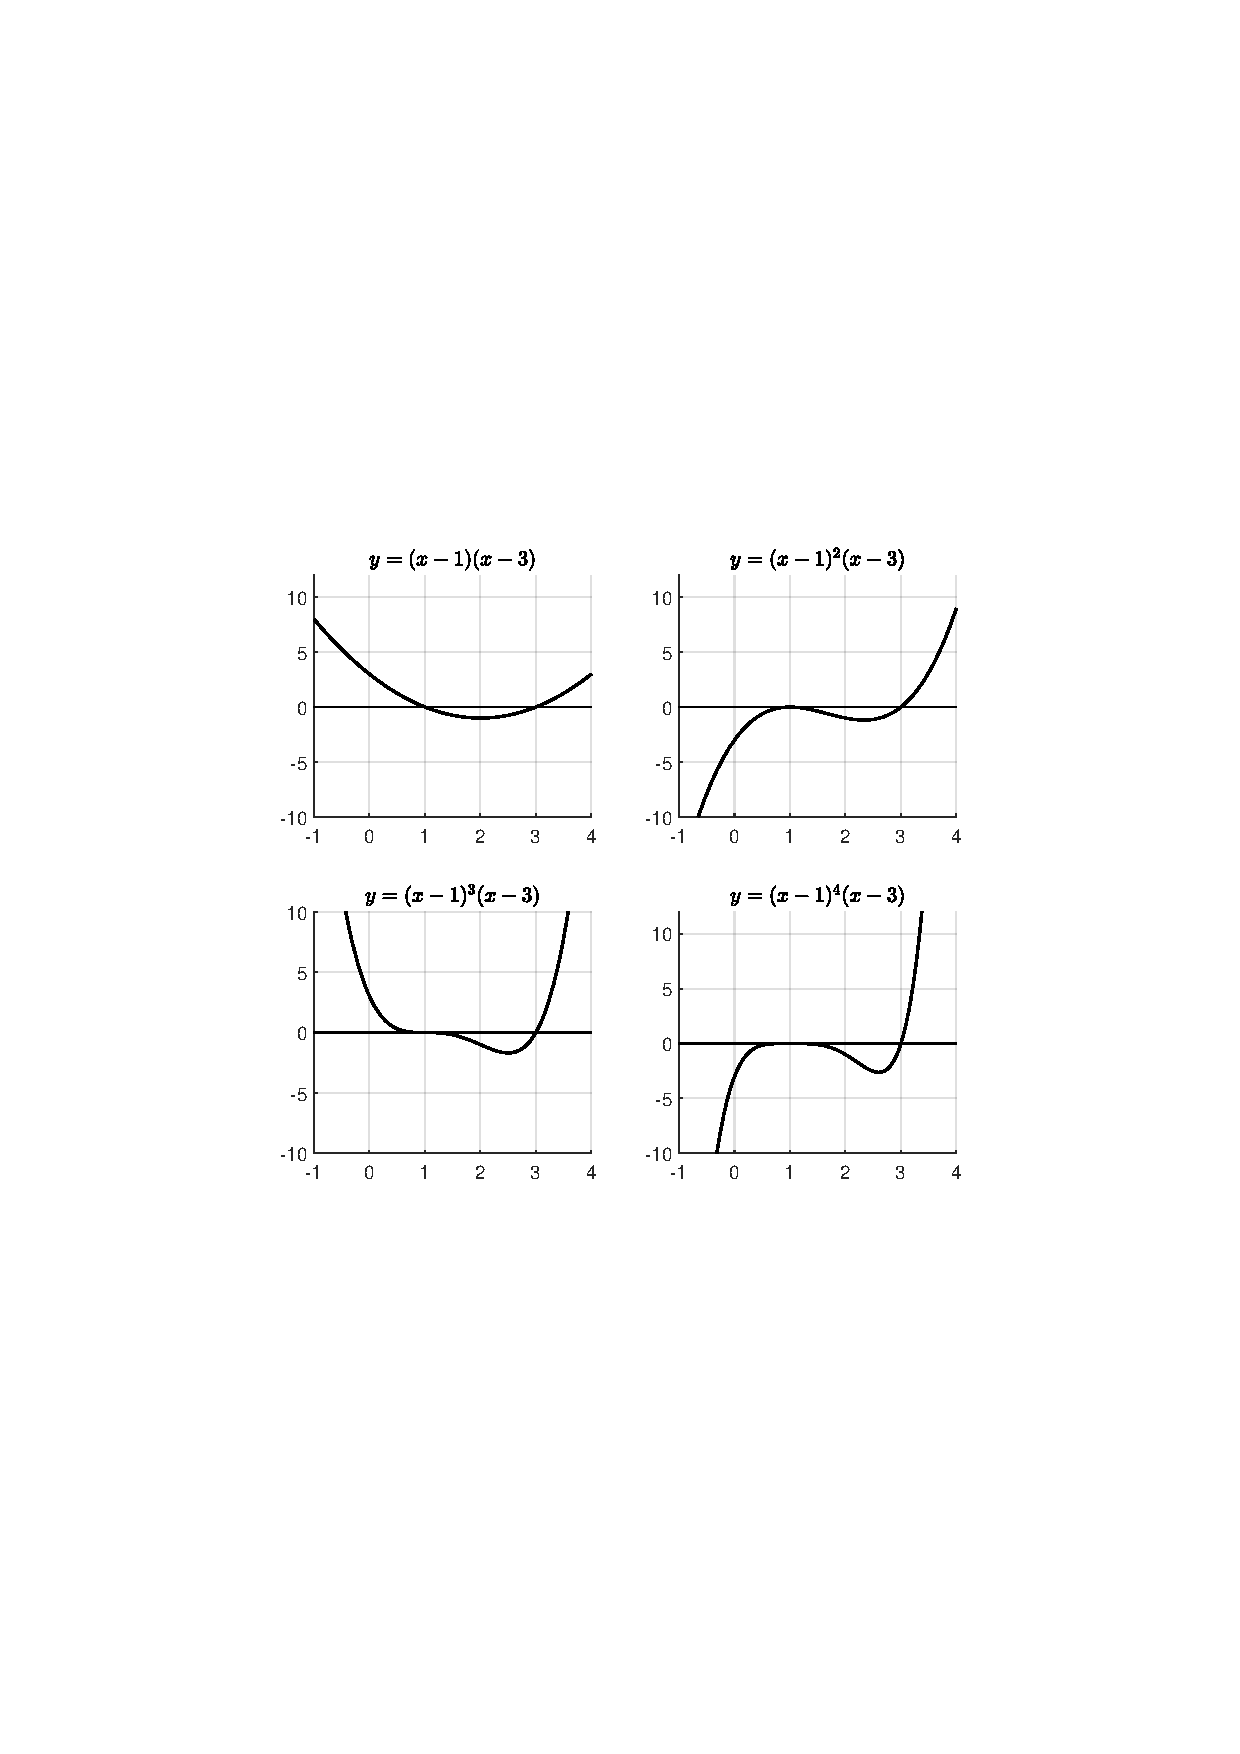
\includegraphics[width=0.6\linewidth]{有重根的多项式与x轴相切}
\end{figure}

\item $^*$ 偏导数是针对含有多个自变量的函数而言的,对某一个自变量求偏导数时,只需要把其它
的自变量看成常数即可。比如$ z=f(x,y)=x^2+xy+y^3+\sin(xy) $,那么
\begin{align*}
    z\ \text{对}\ x\ \text{的偏导数:} &\dfrac{\partial z}{\partial x}=
     2x+y+y\cos(xy) \\
    z\ \text{对}\ y\ \text{的偏导数:} &\dfrac{\partial z}{\partial y}= 
     x+3y^2+x\cos(xy)
\end{align*} 
$ \partial $符号的英文读法是“partial”,中文读法是“偏”。

\item 函数$ y=f(x) $图像上有一点$ P(x_1,f(x_1)) $,函数$ y=g(x) $
图像上有一点$ Q(x_2,g(x_2)) $,求$ |PQ| $的最小值。\\
令$ F(X_1,x_2)=(x_2-x_1)^2+[g(x_2)-f(x_1)]^2 $,
\begin{align}
    & \dfrac{\partial F}{\partial x_1}=-2(x_2-x_1)-2[g(x_2)-f(x_1)]f'(x_1)=0 
    \label{两函数图像距离最小1}  \\
    & \dfrac{\partial F}{\partial x_2}=2(x_2-x_1)+2[g(x_2)-f(x_1)]g'(x_2)=0
    \label{两函数图像距离最小2}
\end{align}
$ \vec{PQ}=(x_2-x_1,g(x_2)-f(x_1)) $,$ P $点的切向量为
$ \vec{t_1}=(1,f'(x_1)) $,$ Q $点的切向量为$ \vec{t_2}=(1,g'(x_2)) $,
(\ref{两函数图像距离最小1})、(\ref{两函数图像距离最小2})式意味着
$  \begin{cases}
    \vec{PQ}\cdot \vec{t_1} =0 \\
    \vec{PQ}\cdot \vec{t_2} =0
\end{cases} $,即$ \vec{PQ}\perp\vec{t_1},\ \vec{PQ}\perp\vec{t_2} $,
$ \vec{t_1}//\vec{t_2} $,这就是$ |PQ| $取得最小值的必要(不充分)条件。

\item 设$ \Delta ABC $的三个顶点的坐标分别为$ (x_i,y_i)\ (i=1,2,3) $,
平面上有一动点$ P(x,y) $,求$ |PA|+|PB|+|PC| $的最小值。\label{费马点求偏导} \\
令$ F(x,y)=\sqrt{(x-x_1)^2+(y-y_1)^2}+\sqrt{(x-x_2)^2+(y-y_2)^2}+
\sqrt{(x-x_3)^2+(y-y_3)^2} $,
\begin{align*}
    &\dfrac{\partial F}{\partial x}=\dfrac{x-x_1}{\sqrt{(x-x_1)^2+(y-y_1)^2}}
    +\dfrac{x-x_2}{\sqrt{(x-x_2)^2+(y-y_2)^2}}+
    \dfrac{x-x_3}{\sqrt{(x-x_3)^2+(y-y_3)^2}}=0 \\
    &\dfrac{\partial F}{\partial y}=\dfrac{y-y_1}{\sqrt{(x-x_1)^2+(y-y_1)^2}}
    +\dfrac{y-y_2}{\sqrt{(x-x_2)^2+(y-y_2)^2}}+
    \dfrac{y-y_3}{\sqrt{(x-x_3)^2+(y-y_3)^2}}=0 
\end{align*}
移项,然后两边平方,
\begin{align*}
    & \Big[\dfrac{x-x_1}{\sqrt{(x-x_1)^2+(y-y_1)^2}}
    +\dfrac{x-x_2}{\sqrt{(x-x_2)^2+(y-y_2)^2}}\Big]^2=
    \Big[-\dfrac{x-x_3}{\sqrt{(x-x_3)^2+(y-y_3)^2}}\Big]^2 \\
    & \Big[\dfrac{y-y_1}{\sqrt{(x-x_1)^2+(y-y_1)^2}}
    +\dfrac{y-y_2}{\sqrt{(x-x_2)^2+(y-y_2)^2}}\Big]^2=
    \Big[-\dfrac{y-y_3}{\sqrt{(x-x_3)^2+(y-y_3)^2}}\Big]^2    
\end{align*}
以上两式相加,
\begin{gather*}
    1+\dfrac{2[(x-x_1)(x-x_2)+(y-y_1)(y-y_2)]}{\sqrt{(x-x_1)^2
            +(y-y_1)^2}\cdot \sqrt{(x-x_2)^2+(y-y_2)^2}}+1=1 \\
    \dfrac{(x-x_1)(x-x_2)+(y-y_1)(y-y_2)}{\sqrt{(x-x_1)^2
            +(y-y_1)^2}\cdot \sqrt{(x-x_2)^2+(y-y_2)^2}}=
    \dfrac{\vec{AP}\cdot \vec{BP}}{|\vec{AP}|\cdot|\vec{BP}|}=
    \cos\angle APB=-\dfrac{1}{2}
\end{gather*}
所以,$ \angle APB=120^{\circ} $. 同理可得$ \angle BPC=\angle CPA
=120^{\circ} $. 当$ \Delta ABC $的最大内角小于$ 120^{\circ} $时,
$ PA,PB,PC $互成$ 120^{\circ} $,$ P $点是$ \Delta ABC $的费马点;
当$ \Delta ABC $的最大内角大于$ 120^{\circ} $时,
$ \angle APB,\angle BPC,\angle CPA $无法同时等于$ 120^{\circ} $,
此时的钝角顶点就是到三个顶点距离之和最小的点。
见本书第\pageref{费马点朝内朝外两种}页的图。

\item 常考函数的导数、极值点和图像。
\begin{table}[h]
\centering
\begin{tabular}{c|ccc}
    函数 & 导数 & 极小值点 & 极大值点 \\
    \hline
    $ x\e^x  $ & $(x+1)\e^x  $ & $(-1,-1/\e)  $ & $ - $ \\
    $ \e^x/x $ & $ (x-1)\e^x/x^2  $ & $ (1,\e) $ & $ - $ \\
    $ x/\e^x $ & $ -(x-1)/\e^x $ & $ - $ & $ (1,1/\e) $ \\
    $ x\ln x $ & $ 1+\ln x $ & $ (1/\e,-1/\e)  $ & $ - $ \\
    $ \ln x/x $ & $ (1-\ln x)/x^2  $ & $ - $ & $ (\e,1/\e)  $ \\
    $ x/\ln x $ & $ (\ln x-1)/\ln^2 x  $ & $ (\e,\e) $ & $ - $ 	
\end{tabular}
\end{table} 
\begin{figure}[h]  % SixFunctionFigure_x_exp_ln.m
    \centering
    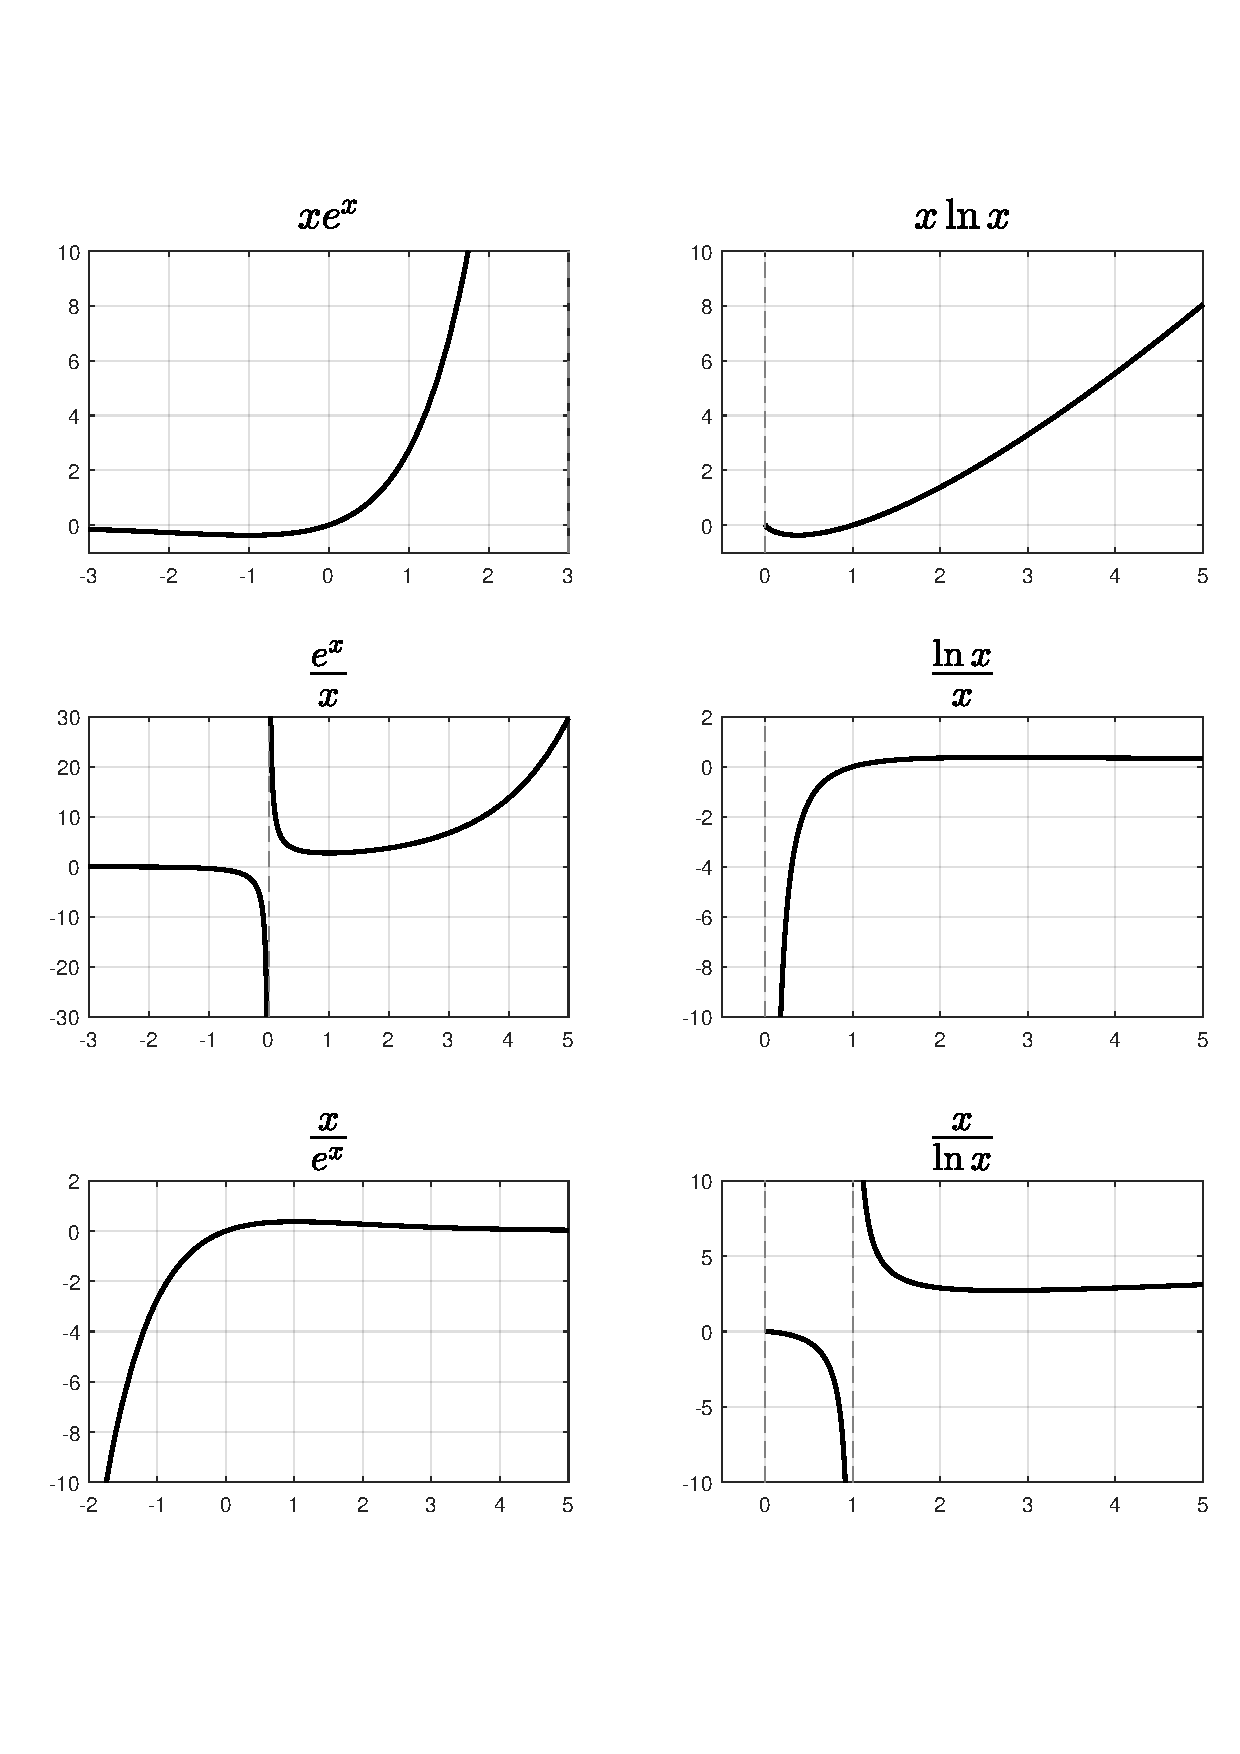
\includegraphics[width=0.6\linewidth]{6个函数图像.pdf}
\end{figure}

\item 把$ \e^x\geq x+1 $中的$ x $换成$ f(x) $,即$ \e^{f(x)} \geq f(x)+1 $,
可以衍生出无穷无尽的不等式,比如把
$ x $换成$ x-1 $,有$ \e^{x-1}\geq x $,
两边同乘$ \e $,有$ \e^x\geq \e x $,这是$ \dfrac{\e^x}{x} $的极小值为
$ \e $的体现,而$ y=\e x $正是$ y=\e^x $在点$ (1,\e) $
处的切线。$ \e^x $的反函数为$ \ln x $,$ \e x $的反函数为$ \dfrac{x}{\e} $,
所以$ \e^x\geq \e x $两边取反函数可得 $ \ln x\leq \dfrac{x}{\e} $.
这是$ \dfrac{\ln x}{x} $的极大值为$ \dfrac{1}{\e} $的体现,
$ y=\dfrac{x}{\e} $是$ y=\ln x $在点$ (\e,1) $处的切线。

\item $ x $换成$ x-\alpha $,有
$ \e^{x-\alpha}\geq x-\alpha+1 $,两边同乘$ \e^{\alpha} $,有
$ \e^x \geq \e^{\alpha}(x-\alpha+1) $.直线$ y=\e^{\alpha}(x-\alpha+1) $
正是$ y=\e^x $在点$ (\alpha,\e^{\alpha}) $处的切线。
取反函数或者取对数后又有新的不等式。

\item $ x $换成$ \alpha x (\alpha>0)$,有
$ \e^{\alpha x}\geq \alpha x+1 $,当$ 1+\alpha x>0 $时,
两边同时开$ \alpha $次方,有$ \e^x\geq (1+\alpha x)^{\frac{1}{\alpha}} $. 

\item $ x $换成$ -\alpha x (\alpha>0)$,有
$ \e^{-\alpha x}\geq -\alpha x+1 $,当$ 1-\alpha x>0 $时,两边同时取倒数,
有$ \e^{\alpha x}\leq \dfrac{1}{1-\alpha x} $,两边同时开$ \alpha $次方,有
$ \e^x \leq \left(\dfrac{1}{1-\alpha x} \right)^{\frac{1}{\alpha}} $. 
当$ \alpha=1 $时,有$ \e^x \leq \dfrac{1}{1-x} $;
当$ \alpha=2 $时,有$ \e^x \leq \sqrt{\dfrac{1}{1-2x}} $;当$ \alpha=\dfrac{1}{2} $时,有$ \e^x \leq \dfrac{1}{(1-\dfrac{x}{2})^2} $. \\
另外,比较幂级数系数也能看出,当$ x \in (0, 1) $时,$ \e^x < \dfrac{1}{1-x} $:
\begin{align*}
    \e^x=1+x+\dfrac{x^2}{2!}+\dfrac{x^3}{3!}+\cdots < 1+x+x^2+x^3+\cdots =\dfrac{1}{1-x}
\end{align*}

\item 当$ x>1 $时,$ \dfrac{x}{\ln x}\geq \e $,$ x\geq \e\ln x $,将
$ x $换成$ x^{1/r}\ (r\in \textbf{R},r>1) $,有
$ x^{1/r}\geq \e\ln x^{1/r}=\dfrac{\e}{r}\ln x $.
(当然,此不等式对于$ r\in(0,1) $也是成立的,但这种左右“相去甚远”的
不等式几乎是毫无用处。)
比如,$ r=2 $时,$ \sqrt{x}\geq \dfrac{\e}{2}\ln x $,
$ \dfrac{2}{\e}\sqrt{x}\geq \ln x $;
$ r=3 $时,$ \sqrt[3]{x}\geq \dfrac{\e}{3}\ln x $,
$ \dfrac{3}{\e}\sqrt[3]{x}\geq \ln x $.

\item $^*$ 函数$ x\ln x $和$ \dfrac{x}{\ln x} $在有关质数的研究中会遇到,
例如,第$ n $个质数的大小大约为$ n[\ln n+\ln(\ln n)-1] $.
\ 第$ 10^8 $个质数是2038074743,
$ 10^8[8\ln 10+\ln(8\ln 10)-1]\approx 2033415473.088 $,相对误差只有0.2$ \% $ .

\item 自然对数的底数$ \e $小于3的证明如下:
\begin{align}
    \left( 1+\dfrac{1}{n}\right)^n =&1+C_n^1\left(\dfrac{1}{n}\right)+
    C_n^2\left(\dfrac{1}{n}\right)^2+\cdots +C_n^n\left(\dfrac{1}{n}\right)^n \nonumber \\
    &<2+\dfrac{1}{2!}+\dfrac{1}{3!}+\dfrac{1}{4!}+\cdots +\dfrac{1}{n!} \nonumber\\
    &<2+\dfrac{1}{2}+\dfrac{1}{2^2}+\dfrac{1}{2^3}+\cdots +\dfrac{1}{2^{n-1}} \quad (n>2,n!>2^{n-1}) \nonumber \\
    =&2+\dfrac{\dfrac{1}{2}-\dfrac{1}{2^n}}{1-\dfrac{1}{2}}=3-\dfrac{1}{2^{n-1}}<3 \label{e小于3的证明}
\end{align}
当$ n>2 $时,$ \left( 1+\dfrac{1}{n}\right)^n =\left(\dfrac{n+1}{n} \right)^n <3  $,即$ 
(n+1)^n<3n^n\leq n^{n+1} $.\ $ 999^{998} < 998^{999} $也可由此证明。

根据均值不等式,
\begin{align*}
    \left( 1+\dfrac{1}{n}\right)^n=1\cdot \left( 1+\dfrac{1}{n}\right)^n 
    <\left[\dfrac{1+n\left(1+\frac{1}{n}\right)}{n+1} \right]^{n+1}
    =\left( 1+\dfrac{1}{n+1}\right)^{n+1}
\end{align*}
说明数列$ \left\{ \left( 1+\dfrac{1}{n}\right)^n \right\}  $是单调递增且有上界的。

$ x\neq 0 $时,
$ 1+x<\e^x $,令$ x=\dfrac{1}{n} $,则$ 1+\dfrac{1}{n}<\e^{1/n} $,
所以$\left( 1+\dfrac{1}{n}\right)^n<\e $.

$ 1-x<\e^{-x} $,令$ x=\dfrac{1}{n+1} $,则$ 1-\dfrac{1}{n+1}=\dfrac{n}{n+1}<\e^{-1/(n+1)},
\dfrac{n+1}{n}>\e^{1/(n+1)} $,所以$ \e < \left( 1+\dfrac{1}{n}\right)^{n+1} $.
于是:
\begin{align}\label{e的两边夹不等式}
    \left( 1+\dfrac{1}{n}\right)^{n} < \e < \left( 1+\dfrac{1}{n}\right)^{n+1}
\end{align}
同时取对数后可得:
\begin{align*}
    \dfrac{1}{n+1} < \ln \dfrac{n+1}{n}=\dfrac{\ln (n+1)-\ln n}{(n+1)-n} < \dfrac{1}{n}
\end{align*}
这个不等式相当于在区间$ [n,n+1] $上对$ \ln x $应用拉格朗日中值定理。

\item 重要例子:绝对值函数$ y=|x| $在\textbf{R}上连续,但在$ x=0 $处不可导。
此例子还能说明,$ \lim\limits_{\Delta x\to 0}\dfrac{f(x+\Delta x)-
f(x-\Delta x)}{2\Delta x} $不能替代$ \lim\limits_{\Delta x\to 0}
\dfrac{f(x+\Delta x)-f(x)}{\Delta x} $作为导数的定义,否则会得出$ y=|x| $
在$ x=0 $处的导数为0的结论。进一步地,$ \lim\limits_{\Delta x\to 0}
\dfrac{f(x+\lambda_1\Delta x)-f(x-\lambda_2\Delta x)}{(\lambda_1+
    \lambda_2)\Delta x} $也不能作为导数的定义。

\item 对于可导函数,$ f'(x_0)=0 $是“$ x=x_0 $为$ f(x) $的
极值点”的必要不充分条件。当$ f'(x_0)=0 $时,\\
\mycircled{1} 若$ f''(x_0)>0 $,则$ x_0 $是$ f(x) $的极小值;\\
\mycircled{2} 若$ f''(x_0)<0 $,则$ x_0 $是$ f(x) $的极大值;\\
\mycircled{3} 若$ f''(x_0)=0 $,则$ x_0 $可能是$ f(x) $的极值点,也可能不是。

比如,$ y=x^3 $和$ y=x^4 $在$ x=0 $处的一阶、二阶导数均为0,$ x_0=0 $不是
$ y=x^3 $的极值点,但是$ y=x^4 $的极小值点。

\item  假设点$ (x_0,y_0) $不在曲线$ y=f(x) $上,要在曲线$ y=f(x) $上找一条经过点$ (x_0,y_0) $的切线,只需求解方程:$ \dfrac{y_0-f(x)}{x_0-x}=f'(x) $. 这一方法也可在圆锥曲线的题目中使用。

\item 对于三次函数$ y=f(x)=ax^3+bx^2+cx+d $,作平移变换$ x=t-\dfrac{b}{3a} $,那么
\begin{align*}
    ax^3+bx^2+cx+d=&\ a\left(t-\dfrac{b}{3a}\right)^3+b\left(t-\dfrac{b}{3a}
    \right)^2+c\left(t-\dfrac{b}{3a}\right)+d\\=&\ at^3+\left(c-\dfrac{b^2}{3a}
    \right)t+\dfrac{2b^3}{27a^2}-\dfrac{bc}{3a}+d
\end{align*}
这样就消去了二次项,剩下的三次函数和一次函数都是中心对称图形,这说明任意三次函数都是
中心对称图形,对称中心的坐标为$ \left(-\dfrac{b}{3a},f\left(-\dfrac{b}{3a}\right)\right) $,对称中心也是三次函数的拐点(二阶导数为0,且二阶导数在此点左右异号)。对三次函数求导,
$ y'=3ax^2+2bx+c $,该二次函数的对称轴是$ x=-\dfrac{b}{3a} $,
与对称中心的横坐标一致。

% SanCiHanShuQieXian.m
\item 从平面上任意一点向三次函数$ y=f(x)=ax^3+bx^2+cx+d $作切线的条数问题。
\begin{figure}[H]
    \centering
    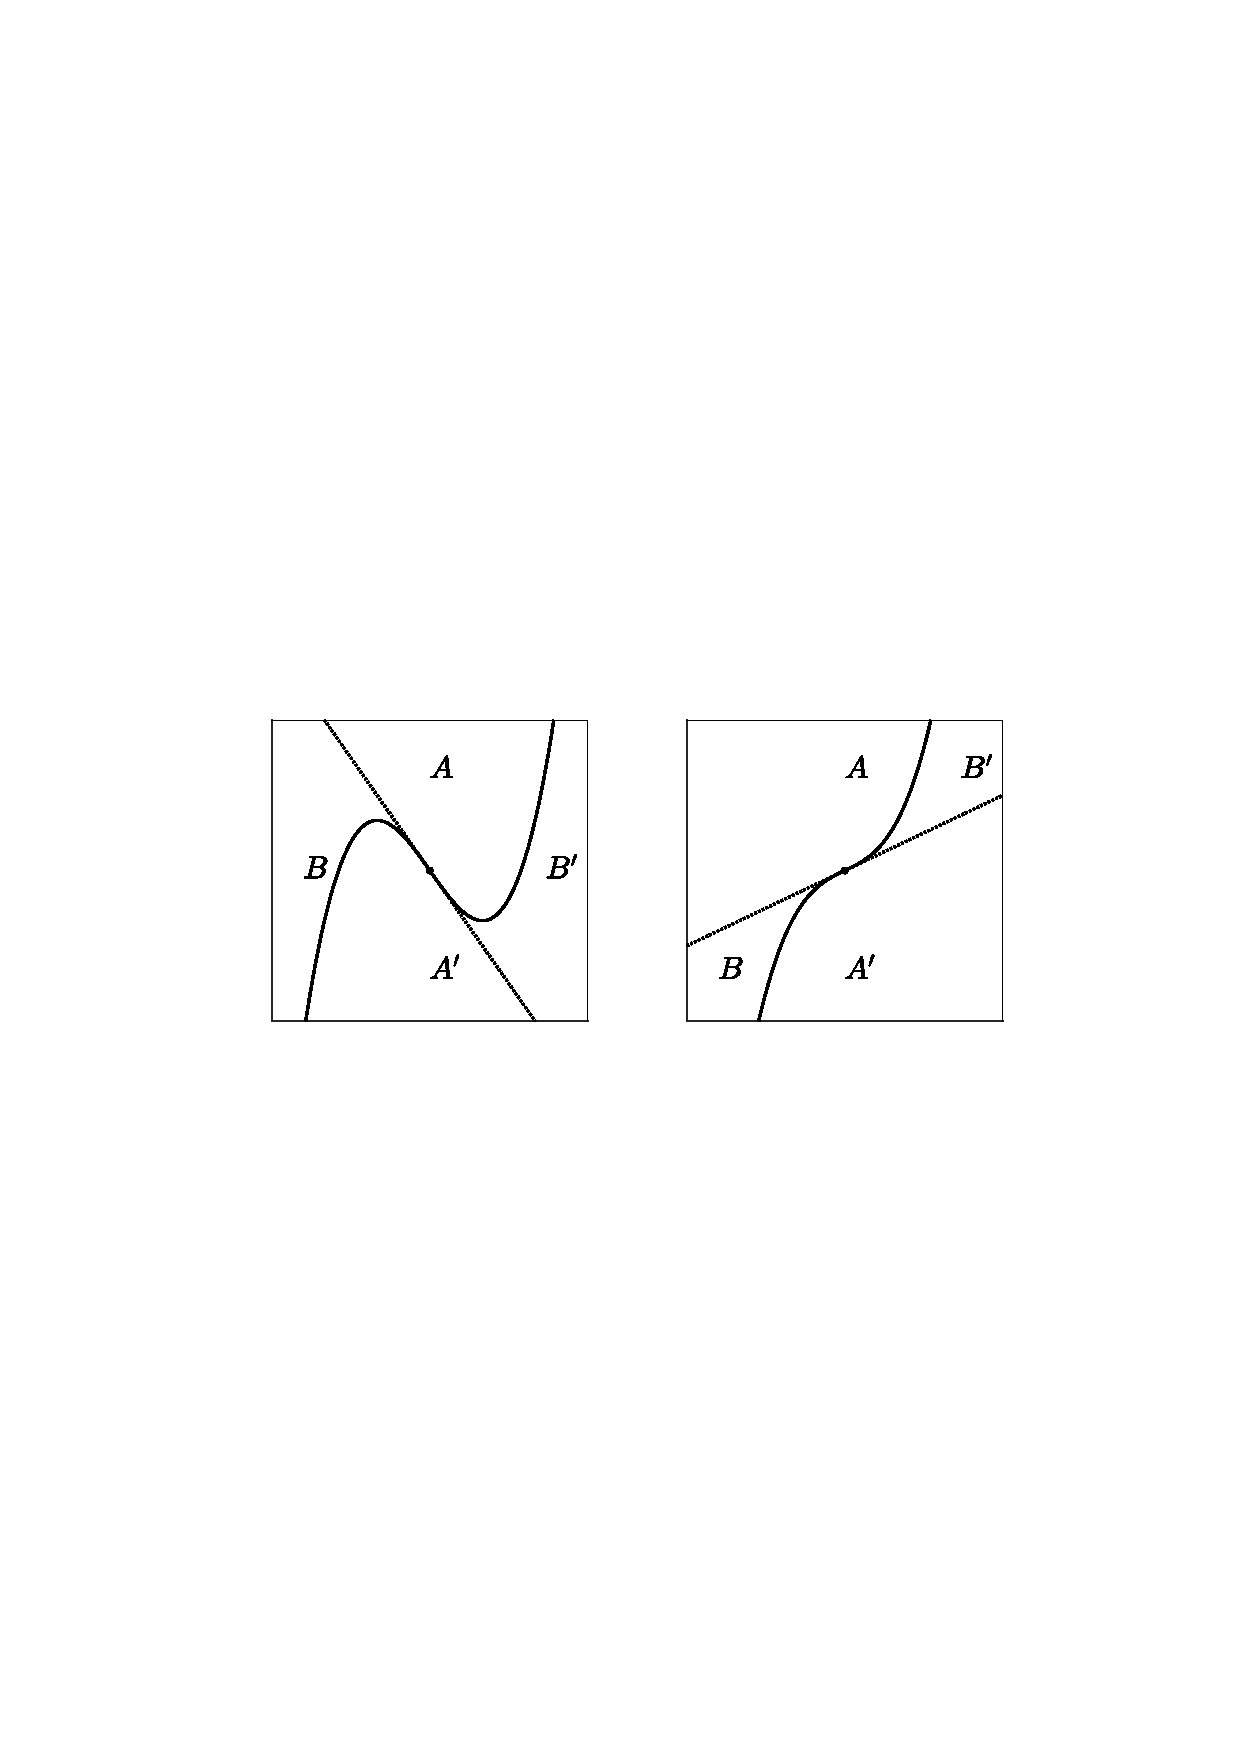
\includegraphics[width=0.7\linewidth]{三次函数切线条数}
\end{figure}

过三次函数对称中心的切线的方程为$ y=\left(c-\dfrac{b^2}{3a}
\right)\left(x+\dfrac{b}{3a}\right)+f\left(-\dfrac{b}{3a}\right) $. 上图中的虚线就是过对称中心的切线,切线与三次曲线将平面分为四个区域,\\
(I) 在$ A $和$ A' $区域,以及对称中心处,只能作1条切线;\\
(II) 在切线和三次曲线上(除对称中心外),能作2条切线;\\
(III) 在$ B $和$ B' $区域能作三条切线。

\item $ ^* $对于3次曲线$ y=f(x)=\dfrac{x+a}{x^2+b}\ (b>0) $,有
\begin{gather*}
    f'(x)=\dfrac{-x^2-2ax+b}{(x^2+b)^2},\q 
    f''(x)=\dfrac{2(x^3+3ax^2-3bx-ab)}{(x^2+b)^3}
\end{gather*}
令$ g(x)=x^3+3ax^2-3bx-ab $,则$ g'(x)=3(x^2+2ax-b) $,
因为$ b>0 $,所以$ g'(x)=0 $的两个实根是
$ r_1=-a-\sqrt{a^2+b},\ r_2=-a+\sqrt{a^2+b} $,
\begin{gather*}
    g(r_1)=2(a^2+b)\left(a+\sqrt{a^2+b}\right)>0 \\
    g(r_2)=2(a^2+b)\left(a-\sqrt{a^2+b}\right)<0 
\end{gather*}
所以$ g(x)=0 $必有3个实根,$ f''(x)=\dfrac{2g(x)}{(x^2+b)^2}=0 $
也有3个实根,即3次曲线$ y=f(x) $有3个拐点。设这3个拐点的坐标
依次为$ (x_i,y_i)\ (i=1,2,3) $,那么$ g(x_i)=x_i^3+3ax_i^2-3bx_i-ab=0 $可
变换成如下形式:
\begin{gather*}
    \dfrac{2x_i}{3x_i^2-b}=\dfrac{x_i+a}{x_i^2+b}=y_i \\
    (3x_i^2-b)y_i=2x_i \\
    (3x_i^2+3b-4b)y_i=3(x_i^2+b)y_i-4by_i=3(x_i+a)-4by_i=2x_i \\
    x_i-4by_i+3a=0
\end{gather*}
这说明,$ (x_i,y_i)\ (i=1,2,3) $三点均在直线$ x-4by+3a=0 $上,
即3次曲线$ y=f(x)=\dfrac{x+a}{x^2+b}\ (b>0) $的3个拐点正好在一条直线上。\\
事实上还有更强的结论:三次曲线的任何两个拐点的连线,
与曲线的第三个交点总是另一个拐点。

\item $^*$ 对任意$ n $次首一多项式$ P(x) $(最高次项系数为1的多项式),设$ M $代表
$ |P(x)| $在区间$ [-1,1] $上的最大值,那么无论其它项的系数怎么变化(保持首一),
$ M $总是大于等于$ \dfrac{1}{2^{n-1}} $. 该结论可借助第一类切比雪夫多项式
$ T_n(\cos x)=\cos nx $进行证明\footnote{证明可参见
    https://zhuanlan.zhihu.com/p/105766114 }。
例如,首一的三次多项式$ |x^3+ax+b| $
在区间$ [-1,1] $上的最大值不小于$ \dfrac{1}{4} $。\\

\end{itemize}

\section{泰勒级数}
\begin{itemize}[leftmargin=\inteval{\myitemleftmargin}pt,itemsep=
   \inteval{\myitemitempsep}pt,topsep=\inteval{\myitemtopsep}pt]
\item $^*$ 函数$ f(x) $在$ x=x_0 $处的泰勒(Taylor)级数
\begin{align*}
    f(x)=&\ f(x_0)+\dfrac{f'(x_0)}{1!}(x-x_0)+\dfrac{f''(x_0)}{2!}
    (x-x_0)^2\\ &\ + \dfrac{f'''(x_0)}{3!}(x-x_0)^3+\cdots+
    \dfrac{f^{(n)}(x_0)}{n!}(x-x_0)^n+\cdots
\end{align*}
特别地,当$ x_0=0 $时,
\begin{align*}
    \e^x=&\ 1+x+\dfrac{x^2}{2!}+\dfrac{x^3}{3!}+\cdots+\dfrac{x^n}{n!}+\cdots \\
    \sin x=&\ x-\dfrac{x^3}{3!}+\dfrac{x^5}{5!}-\cdots +(-1)^n
    \dfrac{x^{2n+1}}{(2n+1)!} +\cdots \\
    \cos x=&\ 1-\dfrac{x^2}{2!}+\dfrac{x^4}{4!}-\cdots +(-1)^n
    \dfrac{x^{2n}}{(2n)!} +\cdots \\
    \tan x=&\ x+\dfrac{1}{3}x^3+\dfrac{2}{15}x^5+\dfrac{17}{315}x^7+\cdots +
    4^n(4^n-1)\dfrac{|B_{2n}|x^{2n-1}}{(2n)!}+\cdots  \\
    \dfrac{1}{1+x}=&\ 1-x+x^2-x^3+\cdots (-1)^{n-1}x^{n-1}+\cdots \\
    \ln(1+x)=&\ x-\dfrac{x^2}{2}+\dfrac{x^3}{3}-\dfrac{x^4}{4}+
    \cdots (-1)^{n-1}\dfrac{x^n}{n}+ \cdots
\end{align*} 
\textbf{注}:$ \tan x $的泰勒级数中的$ B_{2n} $是伯努利数。\\
$ (2k)!!=2k(2k-2)(2k-4)\cdots 6\cdot 4 \cdot 2,
\ (2k+1)!!=(2k+1)(2k-1)(2k-3)\cdots 5\cdot 3\cdot 1 $ . \\
\\
按照二项式定理对$ (1+x)^n $进行展开,与它在$ x_0=0 $处的泰勒展开是一样的。
如果指数不是整数,那么$ (1+x)^{\alpha} $在$ x_0=0 $处的泰勒展开为
\begin{align}\label{牛顿广义二项式定理}
    &\ (1+x)^{\alpha}\nonumber \\ 
    =&\  1+\alpha x+\dfrac{\alpha(\alpha
    -1)}{2!}x^2+\dfrac{\alpha(\alpha-1)(\alpha-2)}{3!}+\cdots+
    \dfrac{\alpha(\alpha-1)\cdots(\alpha-n+1)}{n!}x^n+\cdots 
\end{align}
如果对组合数$ C_n^k $进行推广,允许下标$ n $不是正整数
(但上标$ k $还是正整数),
即$ C_\alpha^k=\dfrac{1}{k!} \alpha(\alpha-1)\cdots
(\alpha-k+1) $,那么(\ref{牛顿广义二项式定理})式可以写成
\begin{gather*}
    (1+x)^{\alpha}= 1+C_{\alpha}^1 x+C_{\alpha}^2 x^2+ 
    C_{\alpha}^3 x^3+\cdots+C_{\alpha}^n x^n +\cdots 
\end{gather*}
前面的一些项保持了与普通二项式定理一致的形式。所以,(\ref{牛顿广义二项式定理})
式也被称为牛顿广义二项式定理。当$ \alpha=\dfrac{1}{2} $时,
\begin{gather*}
    \sqrt{1+x}= 1+\dfrac{1}{2}x-\dfrac{1}{2\cdot 4}x^2+
    \dfrac{1\cdot 3}{2\cdot 4\cdot 6}x^3-\cdots +(-1)^{n-1}\dfrac{(2n-3)!!}
    {(2n)!!}x^n+\cdots
\end{gather*}
\\
泰勒级数可以作为$ f(x) $在$ x=x_0 $附近的近似替代,$ |x-x_0| $越小,
泰勒级数取的项数越多,近似替代的精度就越高。比如:$ x_0=0,\ x=0.1,\ 
\e^{0.1}=1.1051709180\cdots,\ 1+x=1.1,\ 1+x+\dfrac{x^2}{2}=1.105,\  
1+x+\dfrac{x^2}{2}+\dfrac{x^3}{6}=1.10516666,\ 1+x+
\dfrac{x^2}{2}+\dfrac{x^3}{6}+\dfrac{x^4}{24}=1.105170833,\cdots $.

\item 三个数学软件计算泰勒级数的语法 
\begin{table}[H]
%\vspace{-2mm}
\centering
\begin{tabular}{|r|l|}
    \hline
    MATLAB & syms x; taylor(exp(x), x, 0, 'Order', 3) \\ \hline
    Maple & taylor(exp(x), x=0, 3) \\ \hline
    Mathematica & Series[Exp[x], \{x, 0, 3\}] \\ \hline
\end{tabular}
\vspace{-3mm}
\end{table} 
\noindent 其中的0就是$ x_0 $,3就是展开到$ x^{3-1} $或$ x^3 $
(不同软件有区别)。

\item 计算各类函数值的基本方法是利用以泰勒级数为代表的多项式进行逼近,
但是,多项式逼近均具有“局部性”,比如泰勒级数,离展开点越远,
绝对误差就越大。本书将粗略地介绍$ \ln x,\ \e^x,\sin x,\cos x $
的计算方法,而要让代码具有实用价值,还需要使用大量的编程技巧去提高
计算速度和精度\footnote{想要了解这些技术细节,
    可以去阅读一些知名开源项目的源代码。
    微软将Windows系统自带的计算器开源了,
    地址是https://github.com/microsoft/calculator,
    在src\textbackslash CalcManager\textbackslash Ratpack文件夹下,
    exp.cpp文件包括了指数函数和对数函数的C语言实现,
    trans.cpp文件包含了三角函数$ \sin,\cos,\tan $的实现,
    不过阅读难度较大。}。

\item 计算$ \ln x $的基础公式。当$ |t|<1 $时,有等比数列求和公式
\begin{gather*}
    \dfrac{1}{1+t}=1-t+t^2-\cdots+(-t)^{n-1}+\cdots
\end{gather*}
两边在区间$ [0,t] $上积分,可以得到$ \ln(1+t) $的泰勒级数,
\begin{align}\label{ln(1+t)泰勒级数}
    \ln(1+t)=t-\dfrac{t^2}{2}+\dfrac{t^3}{3}-
    \cdots +\dfrac{(-1)^{n-1}t^{n}}{n}+\cdots 
\end{align}
把上式的$ t $换成$ -t $,
\begin{gather}\label{ln(1-t)泰勒级数}
    \ln(1-t)=-t-\dfrac{t^2}{2}-\dfrac{t^3}{3}-
    \cdots -\dfrac{t^{n-1}}{n}-\cdots 
\end{gather}
用(\ref{ln(1+t)泰勒级数})式减去(\ref{ln(1-t)泰勒级数})式,
\begin{align}\label{ln(1+t)_(1-t)幂级数}
    \ln\dfrac{1+t}{1-t}=2\left(t+\dfrac{t^3}{3}+\dfrac{t^5}{5}+\cdots +\dfrac{t^{2k-1}}{2k-1} +\cdots \right)
\end{align}
$ |t| $越小,等号右侧取的项越多,则越精确。
根据上式,当$ t\in(0,1) $时,
\begin{gather}\label{exp(2x)帕德逼近}
    \ln\dfrac{1+t}{1-t}>2t, \quad \quad \dfrac{1+t}{1-t}>\e^{2t} 
\end{gather}
令$ \dfrac{1+t}{1-t}=x $,解得$ t=\dfrac{x-1}{x+1} $,
在(\ref{ln(1+t)_(1-t)幂级数})式等号右侧只取一项,那么
\begin{align} \label{lnt帕德逼近}
    \ln x\approx \dfrac{2(x-1)}{x+1} 
\end{align}
$ \dfrac{2(x-1)}{x+1} $实际上就是$ \ln x $在$ x=1 $处的$ (1,1) $阶帕德(Pade)逼近(下一节将进行介绍),而$ \dfrac{1+t}{1-t} $就是$ \e^{2t} $在$ t=0 $处的的$ (1,1) $阶帕德逼近。\\
在(\ref{ln(1+t)_(1-t)幂级数})式等号右侧取两项,
\begin{align}\label{lnt近似-泰勒取两项}
    \ln x\approx 2\left[\dfrac{x-1}{x+1}+\dfrac{1}{3}\left(
    \dfrac{x-1}{x+1}\right)^3\right]=\dfrac{8(x^3-1)}{3(x+1)^3}=
    \dfrac{(x-1)(8x^2+8x+8)}{3(x^3+3x^2+3x+1)}
\end{align}

不过,上式的精度不如以下的$ (3,3) $阶帕德逼近
\begin{align}\label{lnt帕德近似3_3}
    \ln x \approx&\ \dfrac{11(x-1)^3+60(x-1)^2+60(x-1)}
    {3(x-1)^3+36(x-1)^2 +90(x-1)+60} \nonumber \\ 
    =&\ \dfrac{11x^3+27x^2-27x-11}{3(x^3+9x^2+9x+1)}=
    \dfrac{(x-1)(11x^2+38x+11)}{3(x^3+9x^2+9x+1)}
\end{align}
\begin{figure}[!htbp]
    \centering
    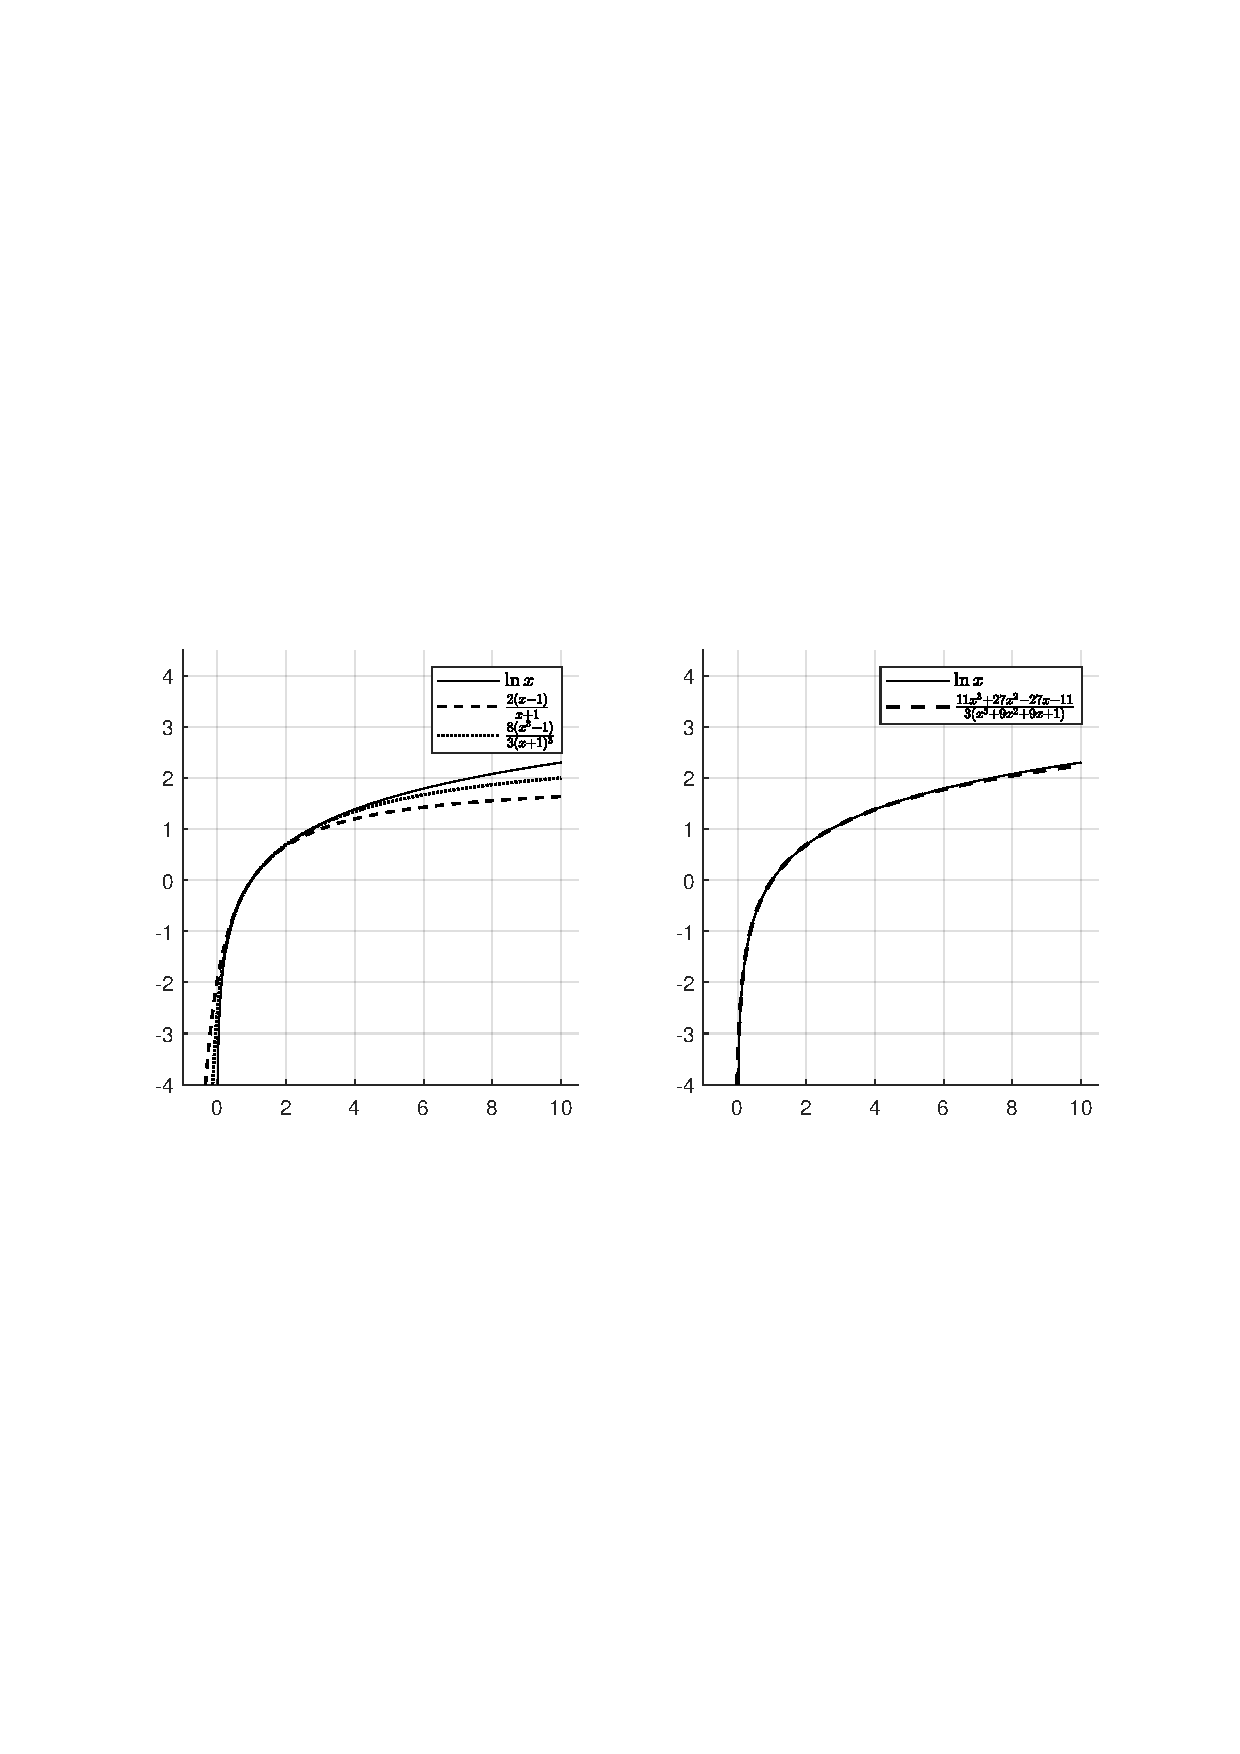
\includegraphics[width=1\linewidth]{lnx帕德逼近}
\end{figure}

\item 手工计算$ \ln x $的方法:选取整数$ k $\ (可正可负),使得
$ \dfrac{x}{2^k}=m $尽可能接近于1,令$ \dfrac{1+t}{1-t}=m $,
那么$ t=\dfrac{m-1}{m+1} $,于是有
\begin{align*}
    \ln x=&\ k\ln 2+\ln m \\
    =&\ k\ln 2+\ln\left(\dfrac{1+t}{1-t}\right) 
    \q\q (\text{利用}\eqref{ln(1+t)_(1-t)幂级数}\text{式}) \\
    =&\ k\ln 2+2\left(t+\dfrac{t^3}{3}+
    \dfrac{t^5}{5}+\cdots\right) \q\q \left(t=\dfrac{m-1}{m+1}\right)
\end{align*}
获取$ n,m $并不困难,但需要熟悉2的整数次幂:
\begin{gather*}
    2^4=16,\q 2^5=32,\q 2^6=64,\q 2^7=128,\q 2^8=256, \\
    2^9=512,\q 2^{10}=1024,\q 2^{11}=2048,\q 2^{12}=4096
\end{gather*}
同时,请大家记住$ \ln 2\approx 0.693147\cdots $
\footnote{2014年新课标全国II卷导数大题考察了求$ \ln2 $的近似值。}. \\ 
现在以$ x=123 $为例,取$ k=7 $,
$ m=\dfrac{123}{128}=\dfrac{1+t}{1-t} $,
$ t=\dfrac{m-1}{m+1}=\dfrac{\frac{123}{128}-1}{\frac{123}{128}+1}
=-\dfrac{5}{251} $,那么
\begin{gather*}
    \ln 123\approx 7\times 0.6931-2\times\dfrac{5}{251}
    \approx 4.8118
\end{gather*}
而$ \ln 123 $的精确值是$ 4.812184\cdots $. 如果不用上面的方法,
而是直接令$ \dfrac{1+t}{1-t}=123 $,
那么$ t=\dfrac{61}{62} $,这个值的绝对值比刚才的
$ -\dfrac{5}{251} $的绝对值大了不少。然后
\begin{gather*}
    \ln 123\approx 2\times \left[\dfrac{61}{62}+\dfrac{1}{3}\cdot 
    \left(\dfrac{61}{62}\right)^3\right] \approx 2.6026
\end{gather*}
这里的计算对手算而言已经十分繁琐了,然而毫无精度可言。 \\
对于$ 3,\ 7 $等接近e的整数次幂的整数,也有另一种估算方法:
\begin{align}
    \ln 3 &=\ln(2.72+0.28)=\ln 2.72+\ln\left(1+\frac{0.28}{2.72}\right)
    \approx 1+\frac{0.28}{2.72}\approx 1.103 \\
    \ln 7 &=\ln(7.29-0.29)=\ln7.29+\ln\Big(1-\frac{0.29}{7.29}\Big)
    \approx 2-\frac{0.29}{7.29}\approx 1.960 \label{ln7估算方法}
\end{align}
下面是3、5、7的自然对数值,读者可以感受一下以上估算的精度,
\begin{gather*}
   \ln3=1.098612\cdots,\q \ln5=1.609438\cdots,\q \ln7=1.945910\cdots
\end{gather*}

\item 编程计算$ \ln x $的方法
\footnote{笔者写了一段简易的C语言程序可做参考
    https://zhuanlan.zhihu.com/p/4742850738 }:
如果$ x\notin (1,2) $,
那就除以$ 2^k $\ ($ k $是整数,可正可负),
使$ \dfrac{x}{2^k}=m\in(1,2) $ .
之所以除以$ 2^k $,是因为可以
利用IEEE 754浮点数的格式,$ k $很容易通过浮点数的阶码获取,
$ m $可以通过浮点数的尾数(mantissa)获取。
尾数的范围是$ [1,2) $,所以才规定$ m\in(1,2) $.
令$ \dfrac{1+t}{1-t}=\dfrac{\sqrt{2}}{2}m\in
\left(\dfrac{\sqrt{2}}{2},\sqrt{2}\right) $,
那么$ t=\dfrac{\frac{\sqrt{2}}{2}m-1}{\frac{\sqrt{2}}{2}m+1}\in
(-(3-2\sqrt{2}), 3-2\sqrt{2}) $.
此时的$ t $的绝对值足够小,而且是落在关于原点对称的区间内。
如果令$ \dfrac{1+t}{1-t} $等于$ m $而不是$ \dfrac{\sqrt{2}}{2}m $,
那么$ t=\dfrac{m-1}{m+1}\in\left(0,\dfrac{1}{3}\right) $,
$ \dfrac{1}{3}\approx 0.3333 > 3-2\sqrt{2}\approx 0.1716 $,
此时$ t $的绝对值不够小,而且所在区间也不是关于原点对称。所以,
在编程时令$ \dfrac{1+t}{1-t}=\dfrac{\sqrt{2}}{2}m $\ (更精确),
而在手工计算时令$ \dfrac{1+t}{1-t}=m $\ (更方便).于是,
\begin{align*}
    \ln x=&\ k\ln 2+\ln m \\
    =&\ k\ln 2+\ln\sqrt{2}+\ln\left(\dfrac{\sqrt{2}}{2}m\right) \\
    =&\ (k+0.5)\ln 2+\ln\left(\dfrac{1+t}{1-t}\right) \\
    =&\ (k+0.5)\ln 2+\left(2t+\dfrac{2t^3}{3}+
    \dfrac{2t^5}{5}+\cdots\right) \q\q 
    \left(t=\dfrac{\frac{\sqrt{2}}{2}m-1}{\frac{\sqrt{2}}{2}m+1}\right)
\end{align*}
$ \ln 2 $会事先算好存起来,在计算机程序中当常数使用。 
多项式求值会采用秦九韶算法,并利用现代CPU中的融合乘加指令
(Fused Multiply-Add, FMA)加速计算。

以其它正实数为底的对数$ \log_a x $,可以通过换底公式
$ \log_a x=\dfrac{\ln x}{\ln a} $转化为自然对数,
分别计算$ \ln x,\ \ln a $,再做除法即可。

\item $ f(x)=\ln\dfrac{1+x}{1-x} $满足函数方程$ f(x_1)+f(x_2)=
f\left(\dfrac{x_1+x_2}{1+x_1x_2}\right) $,
\begin{align*}
    f(x_1)+f(x_2) =\ln\dfrac{(1+x_1)(1+x_2)}{(1-x_1)(1-x_2)}
    &=\ln\dfrac{1+(x_1+x_2)+x_1x_2}{1-(x_1+x_2)+x_1x_2}\\
    &=\ln\dfrac{1+\dfrac{x_1+x_2}{1+x_1x_2}}{1-\dfrac{x_1+x_2}{1+x_1x_2}}=
    f\left(\dfrac{x_1+x_2}{1+x_1x_2}\right) 
\end{align*}

\item 编程计算$ \e^x $的方法
\footnote{笔者写了一段简易的C语言程序可做参考
    https://zhuanlan.zhihu.com/p/4721400461}:
将$ x $写成如下形式:$ x=k_1\ln2 +b_1 $,其中$ k_1 $为整数(可正可负),
$ b_1\in[0,\ln2) $. 相当于将$ x $对$ \ln2 $
进行带余除法,那么
\begin{align*}
    \e^x=\e^{k_1\ln2 +b_1}=\e^{\ln2^{k_1}}\cdot \e^{b_1}=
    2^{k_1}\cdot \e^{b_1}
\end{align*}
因为计算机是二进制的,将一个数(不管是整数还是浮点数)
乘以或除以2的整数次幂是十分容易的(对整数移位或者修改浮点数的阶码)。
于是只需要计算出$ \e^{b_1} $. 因为
$ b_1\in[0,\ln2) $,这个区间还是比较长的,
如果直接使用某种多项式逼近:若多项式的阶数很低,
则逼近精度天然不高。
若多项式的阶数很高,则浮点乘法次数太多导致速度慢,
而且会有更多的误差累积,精度仍然不理想。
所以必须缩短使用多项式拟合的区间,我们可以把前面的
“带余除法”再用一次,令$ b_1=k_2\cdot \dfrac{\ln2}{128}+b_2 $,
其中$ k_2 $为正整数,$ k_2\in[0,127],\ 
b_2\in\left[0,\dfrac{\ln2}{128}\right)$,
$ b_2 $所在的区间就很短了,可以使用低阶的多项式实现高精度的逼近。
\begin{align*}
    \e^{b_1}&=\e^{k_2\cdot\frac{\ln2}{128}}\cdot \e^{b_2} \\
    \e^{b_2}&\approx 1+b_2+\frac{b_2^2}{2!}+\frac{b_2^3}{3!}
    +\frac{b_2^4}{4!}+\frac{b_2^5}{5!} \\
    \e^x&\approx 2^{k_1}\cdot \e^{k_2\cdot\frac{\ln2}{128}}
    \cdot\left(1+b_2+\frac{b_2^2}{2!}+\frac{b_2^3}{3!}
    +\frac{b_2^4}{4!}+\frac{b_2^5}{5!} \right)
\end{align*}
那其中的$ \e^{k_2\cdot\frac{\ln2}{128}}=
\left(2^{1/128}\right)^{k_2} $该怎么计算呢?
答案是提前算好,用一张表(数组)保存起来,要用的时候去查表。
生成这张数表是一劳永逸的操作,可以使用计算代价很大的方法,
比如可以使用128bit的浮点数进行计算(大多数场合
使用64bit浮点数就足够了)。\\
以其它正实数为底的指数函数$ a^x $,可以通过
$ a^x=\e^{x\ln a} $转化为以$ \e $为底的指数函数。\\
因为$ 1024\ln 2=709.7827\cdots $,所以只要
$ x $超过$ 709.7827\cdots $,那么$ \e^x $就会
超过64bit浮点数可表示的最大值$ 2^{1024}=1.797693\times10^{308} $.

\item 第二种编程计算$ \e^x $的方法,特点是编程极其简单,
缺点是精度差,只适用于绝对值比较小的$ x $,
所以本方法通常用在一些低性能的单片机上。利用$ \e $的定义,
\begin{gather*}
    e^x=\lim_{n\to\infty}\left(1+ \dfrac{1}{n}\right)^{nx}\xlongequal{nx=N}
    \lim_{N\to\infty}\left(1+\dfrac{x}{N}\right)^{N}
\end{gather*}
可以选取较大的$ N $来做近似,而当$ N=2^r $\ ($ r $为正整数)时,
尤其方便编程。原因如下,取$ a_1=1+\dfrac{x}{N},\ a_{k+1}=a_k^2 $
(递推公式的含义就是反复地做平方运算),对$ a_1 $进行$ r $次平方以后,
\begin{gather}\label{exp(x)快速算法}
    a_{r+1}=a_r^2=\cdots=a_1^{2^{r}}=\left(1+\dfrac{x}{2^r}\right)^{2^r}=
    \left(1+\dfrac{x}{N}\right)^{N}\approx \e^x
\end{gather}
在实际编程中通常取$ r\geq 10,\ N\geq 1024 $. 以$ r=10 $为例,
编程时只需要写a=1+x/1024,然后再把a=a*a重复写10遍即可
(如果编译器不进行循环展开的优化,那么把a=a*a重复写10遍比使用
for, while等循环语句的运行速度更快),所以说编程极其简单。
$ \e^{15} $的精确值是$ 3.269017\cdots \times 10^6 $,
而用这里的简单算法在$ r=10 $时算出的值是
$ 2.932007\cdots\times10^6 $,
可以看出对于绝对值较大的$ x $的误差之大。

\item 和e有关的一些数值:
\begin{gather*}
    1.6^2=2.56<\e<2.89=1.7^2,\q 1.6<\sqrt{\e}\approx 1.648721<1.7, \\
    \e<2.744=1.4^3,\q \sqrt[3]{\e}\approx 1.395612\approx 1.4, \\    
    \e^2\approx 7.389056,\q  \e^3\approx 20.085536\approx 20.1 ,
    \q \e^4\approx 54.598150\approx 50.6, \\
    \dfrac{1}{2}\ln(2\pi)\approx 0.918938
\end{gather*}

\item 编程计算$\sin(x),\cos(x)$的方法:首先,$\sin(x)$是奇函数,
$\cos(x)$是偶函数,那么只需要考虑$x>0$时的函数值。
其次,对于任意正实数$x$,
$\sin(x),\cos(x)$的值都可以通过这两者在区间$\left[0,
\dfrac{\pi}{4}\right]$内的值得到。
所以,第一步就是将正实数$x$
对$ \dfrac{\pi}{4} $进行带余除法,即
$ x=k_1\cdot\dfrac{\pi}{4}+b_1 $,其中$ k_1 $为满足
$ k_1\cdot\dfrac{\pi}{4}\leq x $的最大正整数,
$ b_1\in\left[0,\dfrac{\pi}{4}\right) $,根据$k_1$除以8的余数
\footnote{在C,C++,C\# 等编程语言中,正整数$k_1$除以$2^n$的余数
    可以通过$k_1$和$2^n-1$进行“位与运算”(\&)高效得到,
    比如$k_1$除以8的余数,可以由$ k_1\ \& \ 7 $得到。}
来选择使用8个公式中的哪一个进行计算:
\begin{align*}
    \sin(x)=\sin\left(b_1+k_1\cdot \dfrac{\pi}{4}\right) & =
    \begin{cases}
        \sin(b_1),  &  k_1=8n \\
        \cos\left(\dfrac{\pi}{4}-b_1\right), & k_1=8n+1 \\
        \cos(b_1),  & k_1=8n+2 \\
        \sin\left(\dfrac{\pi}{4}-b_1\right), & k_1=8n+3 \\
        -\sin(b_1),  & k_1=8n+4 \\
        -\cos\left(\dfrac{\pi}{4}-b_1\right), & k_1=8n+5 \\
        -\cos(b_1),  & k_1=8n+6 \\
        -\sin\left(\dfrac{\pi}{4}-b_1\right), & k_1=8n+7 \\
    \end{cases} \\
    \cos(x)=\cos\left(b_1+k_1\cdot \dfrac{\pi}{4}\right) & =
    \begin{cases}
        \cos(b_1),  &  k_1=8n \\
        \sin\left(\dfrac{\pi}{4}-b_1\right), & k_1=8n+1 \\
        -\sin(b_1),  & k_1=8n+2 \\
        -\cos\left(\dfrac{\pi}{4}-b_1\right), & k_1=8n+3 \\
        -\cos(b_1),  & k_1=8n+4 \\
        -\sin\left(\dfrac{\pi}{4}-b_1\right), & k_1=8n+5 \\
        \sin(b_1),  & k_1=8n+6 \\
        \cos\left(\dfrac{\pi}{4}-b_1\right), & k_1=8n+7 \\
    \end{cases}
\end{align*}
再将$b_1$对$\dfrac{\pi}{128}$进行带余除法,
$ b_1=k_2\cdot \dfrac{\pi}{128}+b_2 $,其中$ k_2 $为正整数,
$ k_2\in[0,31] $,$b_2\in\left[0,\dfrac{\pi}{128}\right) $,
$b_2$所在的区间就很短了,可以使用低阶的泰勒级数进行逼近。于是,
\begin{align*}
    \sin(b_1) =&\ \sin\left(k_2\cdot \dfrac{\pi}{128}+b_2\right)
    =\sin\left(k_2\cdot \dfrac{\pi}{128}\right)\cos(b_2)+
    \cos\left(k_2\cdot \dfrac{\pi}{128}\right)\sin(b_2)  \\
    \cos(b_1) =&\ \cos\left(k_2\cdot \dfrac{\pi}{128}+b_2\right)
    =\cos\left(k_2\cdot \dfrac{\pi}{128}\right)\cos(b_2)-
    \sin\left(k_2\cdot \dfrac{\pi}{128}\right)\sin(b_2)  \\   
    \sin(b_2) \approx &\ b_2-\dfrac{b_2^3}{3!}+\dfrac{b_2^5}{5!} \\
    \cos(b_2) \approx &\ 1-\dfrac{b_2^2}{2!}+\dfrac{b_2^4}{4!}-
    \dfrac{b_2^{6}}{6!}
\end{align*}
其中的$ \sin\left(k_2\cdot\dfrac{\pi}{128}\right) $,
$\cos\left(k_2\cdot\dfrac{\pi}{128}\right)$也是事先计算好,
用数组保存起来,要用的时候去查表。\\
手工计算依然只需考虑$\left[0,\dfrac{\pi}{4}\right]$内的角
$ \left(\dfrac{\pi}{4}\approx 0.785\right) $,然后直接使用泰勒级数
的至少两项:
\begin{align}
    \sin(x) \approx &\ x-\dfrac{x^3}{3!} \label{sinx=x-x^3_6}\\
    \cos(x) \approx &\ 1-\dfrac{x^2}{2!} \label{cosx=1-x^2_2}
\end{align}
比如估算$\sin(0.6)$和$\cos(0.6)$,
\begin{align*}
    \sin(0.6) \approx &\ 0.6-\dfrac{0.6^3}{3!}=0.564 
    \q (\text{精确值为} 0.564642\cdots)   \\
    \cos(0.6) \approx &\ 1-\dfrac{0.6^2}{2!}=0.82   
    \q (\text{精确值为} 0.825335\cdots)   
\end{align*}
估算$\sin(0.76)$和$\cos(0.76)$,
\begin{align*}
    \sin(0.76) \approx &\ 0.76-\dfrac{0.76^3}{3!}\approx 0.687 
    \q (\text{精确值为} 0.688921 \cdots)   \\
    \cos(0.76) \approx &\ 1-\dfrac{0.76^2}{2!}=0.7112  
    \q (\text{精确值为} 0.724836 \cdots)     
\end{align*}

\item 常用平方根:
\begin{gather*}
    \sqrt{2}\approx1.414,\ \sqrt{3}\approx1.732,\ \sqrt{5}\approx2.236,\ 
    \sqrt{6}\approx2.449,\ \sqrt{7}\approx2.646,\ \sqrt{10}\approx3.162
\end{gather*}
\\
常用平方数:
\begin{table}[H]
    \centering
    \begin{tabular}{|c|c|c|c|c|}
        \hline
        $ 11^2=121 $ & $ 12^2=144 $ & $ 13^2=169 $ & $ 14^2=196 $ & $ 15^2=225 $\\ \hline
        $ 16^2=256 $ & $ 17^2=289 $ & $ 18^2=324 $ & $ 19^2=361 $ & $ 20^2=400 $\\ \hline
        $ 21^2=441 $ & $ 22^2=484 $ & $ 23^2=529 $ & $ 24^2=576 $ & $ 25^2=625 $\\ \hline
        $ 26^2=676 $ & $ 27^2=729 $ & $ 28^2=784 $ & $ 29^2=841 $ & $ 30^2=900 $\\ \hline
        $ 31^2=961 $ & $ 32^2=1024 $ & $ 33^2=1089 $ & $ 34^2=1156 $ & $ 35^2=1225 $\\ \hline
    \end{tabular}
\end{table}
% \bigskip 
\item 开二次方的估算方法:假设要估算$ \sqrt{a}\ (a>0) $,
可先找出正整数$ k $,满足$ k^2<a<(k+1)^2 $. \\
\mycircled{1}割线法:在函数$ y=\sqrt{x} $上取两点$ (k^2,k) $
和$ ((k+1)^2,k+1) $,用过这两点的割线\\ $ y-k=\dfrac{
    (k+1)-k}{(k+1)^2-k^2}(x-k^2) $来近似代替函数$ y=\sqrt{x} $
在区间$ (k^2,(k+1)^2) $内的部分,所以
$ \sqrt{a}\approx k+\dfrac{a-k^2}{2k+1} $,结果偏小。 \\
\mycircled{2}切线法:在函数$ y=\sqrt{x} $上,用过点$ (k^2,k) $的切线$ y-k=\dfrac{1}{2k}(x-k^2) $来近似代函数$ y=\sqrt{x} $
在区间$ (k^2,(k+1)^2) $内的部分,所以,
$ 	\sqrt{a} \approx k+\dfrac{a-k^2}{2k}=
\dfrac{1}{2}\left(k+\dfrac{a}{k}\right) $,结果偏大。 

结合\mycircled{1}和\mycircled{2}可以看出,
$ k+\dfrac{a-k^2}{2k+0.5} $是更好的近似。切线法实际上是只取了泰勒级数的前两项,即$ f(x)=\sqrt{x} \approx f(x_0)+f'(x_0)(x-x_0) $,如果取更多的项,比如$ \dfrac{f''(x_0)}{2!}(x-x_0)^2,
\dfrac{f'''(x_0)}{3!}(x-x_0)^3\cdots $,就能获得更高的精度。\\
\mycircled{3}将切线法迭代使用(这也是在计算机中求平方根的方法)。
记$ \varphi(x)=\dfrac{1}{2}\left(x+\dfrac{a}{x}\right) $,
那么$ \varphi(x) $的不动点
\footnote{不动点就是方程$ x=\varphi(x) $的根,
参见本书第\ref{sec数列}章“数列”的“不动点”小节。}和极小值点\footnote{
考虑函数$ g(x)=Ax+\dfrac{B}{x}\ (A,B>0) $,其不动点是$ \sqrt{\dfrac{B}{1-A}} $,
只要让$ \sqrt{\dfrac{B}{1-A}}=\sqrt{a} $,
那么迭代数列$ a_{n+1}=g(a_n)=Aa_n+\dfrac{B}{a_n} $就会收敛到$ \sqrt{a} $.
$ g(x) $的极小值点是$ x=\sqrt{\dfrac{B}{A}} $,
如果让不动点与极小值点重合,那么迭代数列$ a_{n+1}=g(a_n) $的收敛速度是最快的。
令$ \sqrt{\dfrac{B}{1-A}}=\sqrt{\dfrac{B}{A}}=\sqrt{a} $,
那么$ A=\dfrac{1}{2},\ B=\dfrac{a}{2},\ g(x)=\dfrac{1}{2}\left(
x+\dfrac{a}{x}\right) $,此时,$ g(x) $恰好与切线法的形式一致。}
都是$ x=\sqrt{a} $.定义数列$ \{a_n\} $,
令$\ a_1=k,\ a_{n+1}=\varphi(a_n)=\dfrac{1}{2}\left(
a_n+\dfrac{a}{a_n}\right) $. 通过不断地迭代计算$ a_n $,
就能逐步逼近$ \sqrt{a} $.
容易验证,$ a_{2}=\dfrac{1}{2}\left(a_1+\dfrac{a}{a_1}\right)
=\dfrac{1}{2}\left(k+\dfrac{a}{k}\right)
\in (\sqrt{a},\sqrt{a}+\dfrac{1}{2}) $.
%\mycircled{3}迭代法:$ 0<A<1,B>0 $,数列$ a_{n+1}=Aa_n+\dfrac{B}{a_n} $的不动点
%\footnote{参见本书第\ref{sec数列}章“数列”的“不动点”小节。}是
%$ \sqrt{\dfrac{B}{1-A}} $,只要让$ A,B $满足$ \sqrt{\dfrac{B}{1-A}}=\sqrt{a} $,
%就可以通过不断计算$ a_n $来逼近$ \sqrt{a} $.如果让函数$ Ax+\dfrac{B}{x} $的
%不动点恰好是它的极小值点($ x=\sqrt{\dfrac{B}{A}} $),那么迭代收敛的速度是最快的。即
%$ \sqrt{\dfrac{B}{1-A}}=\sqrt{\dfrac{B}{A}}=\sqrt{a} $,所以$ A=\dfrac{1}{2},
%B=\dfrac{a}{2} $.选取$ a_1=k $,那么$ a_2=\dfrac{1}{2}\left(a_1+\dfrac{a}{a_1}\right)=
%\dfrac{1}{2}\left(k+\dfrac{a}{k}\right) $,这与切线法的结果一样。按照
%$ a_{n+1}=\dfrac{1}{2}a_n+\dfrac{a}{2a_n} $
%继续计算$ a_3,a_4\cdots $,便能不断提高精度。
下面用数学归纳法证明数列$ \{a_n\} $确实收敛到$ \sqrt{a} $.
假设$ \sqrt{a}<a_n<\sqrt{a}+\dfrac{1}{2^{n-1}}\ (n\geq 2) $,
那么$ \dfrac{1}{a_n} < \dfrac{1}{\sqrt{a}} $,
\begin{align*}
    & a_{n+1}=\dfrac{1}{2}\left(a_n+\dfrac{a}{a_n}\right)>
    \sqrt{a_n\cdot\dfrac{a}{a_n}}=\sqrt{a} \\ 
    & a_{n+1}=\dfrac{1}{2}a_n+\dfrac{a}{2a_n}<\dfrac{1}{2}
    \left(\sqrt{a}+\dfrac{1}{2^{n-1}} \right)+\dfrac{a}{2}\cdot \dfrac{1}{\sqrt{a}}=\sqrt{a}+\dfrac{1}{2^n}
\end{align*}
实际上,数列$ a_n $的通项公式是可以计算出来的,
见本书第\ref{sec数列}章的(\ref{根式迭代序列的通项})式。 

\item $^*$ 开三次方的估算:假设要估算$ \sqrt[3]{a} $,
先找出正整数$ k $,满足$ k^3<a<(k+1)^3 $. \\
\mycircled{1}割线法:$ \sqrt[3]{a}\approx k+\dfrac{a-k^3}{3k^2+3k+1} $,结果偏小。 	\\
\mycircled{2}切线法:$ \sqrt[3]{a}\approx k+\dfrac{a-k^3}{3k^2}=\dfrac{1}{3}\left(2k+\dfrac{a}{k^2}\right) $,结果偏大。\\
\mycircled{3}将切线法迭代使用。定义数列$ \{a_n\} $,令$\ a_1=k,\ a_{n+1}=\dfrac{1}{3}\left(2a_n+\dfrac{a}{a_n^2}\right) $,
那么该数列的不动点是$ \sqrt[3]{a} $,函数$ y=\dfrac{1}{3}\left(2x+\dfrac{a}{x^2}\right) $的极小值点
\footnote{考虑函数$ g(x)=Ax+\dfrac{B}{x^2}\ (A,B>0) $,其不动点是
$ \sqrt[3]{\dfrac{B}{1-A}} $,只要让$ \sqrt[3]{\dfrac{B}{1-A}}=\sqrt[3]{a} $,
那么迭代数列$ a_{n+1}=g(a_n)=Aa_n+\dfrac{B}{a_n^2} $就会收敛到$ \sqrt[3]{a} $.
为求其极小值点,利用三变量均值不等式,
$ Ax+\dfrac{B}{x^2}=\dfrac{1}{2}Ax+\dfrac{1}{2}Ax+\dfrac{B}{x^2}\geq 
3\sqrt[3]{\dfrac{1}{2}Ax\cdot\dfrac{1}{2}Ax\cdot\dfrac{B}{x^2}}=3\sqrt[3]{
    \dfrac{A^2B}{4}} $,当$ \dfrac{1}{2}Ax=\dfrac{B}{x^2},\ x=\sqrt[3]{
    \dfrac{2B}{A}} $时,取得极小值。
如果让不动点与极小值点重合,那么迭代数列$ a_{n+1}=g(a_n) $的收敛速度是最快的。
令$ \sqrt[3]{\dfrac{B}{1-A}}=\sqrt[3]{\dfrac{2B}{A}}=\sqrt[3]{a} $,
那么$ A=\dfrac{2}{3},\ B=\dfrac{a}{3},\ g(x)=\dfrac{1}{3}\left(
2x+\dfrac{a}{x^2}\right) $,此时,$ g(x) $恰好与切线法的形式一致。
2011年上海春季高考的数列大题,
是用$ a_{n+1}=\dfrac{1}{2}\left(a_n+\sqrt{\dfrac{a}{a_n}}\right) $
来获得$ \sqrt[3]{a} $的近似值。}也恰好是$ x=\sqrt[3]{a} $.
    
%\mycircled{3}迭代法:$ a_{n+1}=Aa_n+\dfrac{B}{a_n^2} $,该数列的不动点是
%$ \sqrt[3]{\dfrac{B}{1-A}} $,极小值点\footnote{$ A>0,B>0 $,利用三变量均值不等式,
%$ Ax+\dfrac{B}{x^2}=\dfrac{1}{2}Ax+\dfrac{1}{2}Ax+\dfrac{B}{x^2}\geq 
%3\sqrt[3]{\dfrac{1}{2}Ax\cdot\dfrac{1}{2}Ax\cdot\dfrac{B}{x^2}}=3\sqrt[3]{
%\dfrac{A^2B}{4}} $,当$ \dfrac{1}{2}Ax=\dfrac{B}{x^2},\ x=\sqrt[3]{
%\dfrac{2B}{A}} $时,取得极小值。}是$ \sqrt[3]{\dfrac{2B}{A}} $,同样地,
%让不动点恰好是它的极小值点,$ \sqrt[3]{\dfrac{B}{1-A}}=
%\sqrt[3]{\dfrac{2B}{A}}=\sqrt[3]{a} $,
%$ A=\dfrac{2}{3},B=\dfrac{a}{3} $,$ a_{n+1}=\dfrac{1}{3}\left(2a_n+
%\dfrac{a}{a_n^2}\right) $,$ 
%a_1=k,a_2=\dfrac{1}{3}\left(2k+\dfrac{a}{k^2}\right),\cdots $,与切线法一样。\\
%\myfootnote{\ \ 2011年上海春季高考的数列大题,是用$ a_{n+1}=\dfrac{1}{2}\left(a_n+
%    \sqrt{\dfrac{a}{a_n}}\right) $来获得$ \sqrt[3]{a} $的近似值。}


\end{itemize}

\section{帕德逼近}
\begin{itemize}[leftmargin=\inteval{\myitemleftmargin}pt,itemsep=
   \inteval{\myitemitempsep}pt,topsep=\inteval{\myitemtopsep}pt]
\item 帕德(Pade)逼近\footnote{可查阅Wolfram 
MathWorld上的Pade Approximant条目。}:在某个$ x_0 $附近,
用有理函数(分子分母都是多项式)
\begin{gather*}
    R_{m,n}(x)=\dfrac{a_mx^m+a_{m-1}x^{m-1}+\cdots+a_1x+a_0}
    {b_nx^n+b_{n-1}x^{n-1}+\cdots+b_1x+b_0}
\end{gather*}
去逼近$ f(x) $,将$ R_{m,n}(x) $称为$ f(x) $的$ (m,n) $阶帕德逼近。

计算帕德逼近的系数有如下两种方法:\\
\textbf{方法一}(推荐)\ 先将$ f(x) $在$ x_0 $处展开成泰勒级数,
$ f(x)=c_0+c_1x+c_2x^2+\cdots $,然后
\begin{gather*}
    c_0+c_1x+c_2x^2+\cdots=
    \dfrac{a_mx^m+a_{m-1}x^{m-1}+\cdots+a_1x+a_0}
    {b_nx^n+b_{n-1}x^{n-1}+\cdots+b_1x+b_0} \\
    (c_0+c_1x+c_2x^2+\cdots)(b_0+b_1x+\cdots+b_nx^n)=
    a_0+a_1x+\cdots+a_mx^m \\
    c_0b_0+(c_0b_1+c_1b_0)x+(c_0b_2+c_1b_1+c_2b_0)x^2+\cdots
    =a_0+a_1x+\cdots+a_mx^m
\end{gather*}
让左右两侧同次幂系数相等,即
\begin{align*}
    \begin{cases}
        c_0b_0=a_0 \\
        c_0b_1+c_1b_0=a_1 \\
        c_0b_2+c_1b_1+c_2b_0=a_2 \\
        c_0b_3+c_1b_2+c_2b_1+c_3b_0=a_3 \\
        c_0b_4+c_1b_3+c_2b_2+c_3b_1+c_4b_0=a_4 \\
        \q\q \vdots
    \end{cases}
\end{align*}
以上共有$ m+n+1 $个方程。
不妨假设$ b_0=1 $(举个例子,假设$ b_0\neq 0 $,那么
$ \dfrac{a_1x+a_0}{b_1x+b_0}=\dfrac{\frac{a_1}{b_0}x+
    \frac{a_0}{b_0}}{\frac{b_1}{b_0}x+1} $,所以可以直接设$ b_0=1 $),
然后求解以上方程组即可。如果假设$ b_0=1 $后出现了不可能成立的方程组,
那就假设其它的未知系数为1,比如设$ b_1=1 $. \\
\textbf{方法二}(不推荐)\ 解如下方程组
\begin{align*}
    \begin{cases}
        f(x_0)=R_{m,n}(x_0) \\
        f'(x_0)=R_{m,n}'(x_0) \\
        f''(x_0)=R_{m,n}''(x_0) \\
        f'''(x_0)=R_{m,n}'''(x_0) \\
        \q\q\vdots \\
        f^{(m+n)}(x_0)=R_{m,n}^{(m+n)}(x_0)
    \end{cases}
\end{align*}
以上共有$ m+n+1 $个方程。
因为对$ R_{m,n}(x) $求导比较麻烦,所以不如方法一方便。

\item 以$ f(x)=\e^x $为例,计算在$ x=0 $处的$ (2,2) $阶帕德逼近。\\
\textbf{方法一}\ 设$ R_{2,2}(x)=\dfrac{a_0+a_1x+a_2x^2}{1+b_1x+b_2x^2} $,则
$ c_0=1 $,$ c_1=1 $,$ c_2=\dfrac{1}{2} $,
$ c_3=\dfrac{1}{6} $,$ c_4=\dfrac{1}{24}\cdots $,
\begin{gather*}
    \begin{cases}
        c_0=a_0 \\
        c_0b_1+c_1=a_1 \\
        c_0b_2+c_1b_1+c_2=a_2 \\
        c_1b_2+c_2b_1+c_3=a_3=0 \\
        c_2b_2+c_3b_1+c_4=a_4=0
    \end{cases} \Rightarrow 
    \begin{cases}
        1=a_0 \\
        b_1+1=a_1 \\
        b_2+b_1+\dfrac{1}{2}=a_2 \\
        b_2+\dfrac{1}{2}b_1+\dfrac{1}{6}=0 \\
        \dfrac{1}{2}b_2+\dfrac{1}{6}b_1+\dfrac{1}{24}=0
    \end{cases}
\end{gather*}
解得,$ b_1=-\dfrac{1}{2},\ b_2=\dfrac{1}{12} $,$ a_0=1,\ 
a_1=\dfrac{1}{2},\ a_2=\dfrac{1}{12} $.所以,
\begin{gather*}
    R_{2,2}(x)=\dfrac{1+\dfrac{1}{2}x+\dfrac{1}{12}x^2}{1
        -\dfrac{1}{2}x+\dfrac{1}{12}x^2}=
    \dfrac{12+6x+x^2}{12-6x+x^2}
\end{gather*}
方法二计算过于繁琐,在此略去。

\item 三个数学软件计算帕德逼近的语法 
\begin{table}[!htbp]
%\vspace{-2mm}
\centering
\begin{tabular}{|r|l|}
    \hline
    MATLAB & syms x; pade(exp(x), x, 'Order', [2, 3]) \\ \hline
    Maple & with(numapprox): pade(exp(x), x, [2, 3]) \\ \hline
    Mathematica & PadeApproximant[Exp(x), \{x, 0, \{2, 3\}\}] \\ \hline
\end{tabular}
%\vspace{-3mm}
\end{table} \\
其中的[2, 3]或\{2, 3\}就是$ (m,n) $.

\item $ f(x)=\e^x $在$ x=0 $处的$ (0,0)\sim(3,3) $阶帕德逼近表。
\begin{table}[H]
%\vspace{-2mm}
\centering
\begin{tabular}{|c|c|c|c|c|}
    \hline
\diagbox[width=3em,height=2.1em]{$ n $}{$ m $} & 0 & 1 & 2 & 3 \\
\hline
0 & $ \frac{1}{1} $ & $ \frac{x+1}{1} $ & $ \frac{x^2+2x+2}{2} $ & $ \frac{x^3+3x^2+6x+6}{6} $ \\ \hline
1 & $ \frac{1}{-x+1} $ & $ \frac{x+2}{-x+2} $ & $ \frac{x^2+4x+6}{-2x+6} $ & $ \frac{x^3+6x^2+18x+24}{-6x+24} $  \\ \hline
2 & $ \frac{2}{x^2-2x+2} $ & $ \frac{2x+6}{x^2-4x+6} $ & $ \frac{x^2+6x+12}{x^2-6x+12} $ & $ \frac{x^3+9x^2+36x+60}{3x^2-24x+60} $ \\ \hline
3 & $ \frac{6}{- x^3+3x^2-6x+6} $ & $ \frac{6x+24}{- x^3+6x^2-18x+24} $ & $ \frac{3x^2+24x+60}{- x^3+9x^2-36x+60} $ & $ \frac{x^3+12x^2+6x+120}{- x^3+12x^2-6x+120} $ \\ \hline
\end{tabular}
%\vspace{-2mm}
\end{table}

从表中可以看出$ n=0 $(分母为常数)时的帕德逼近就是泰勒级数。
表中关于主对角线对称(比如$ (2,0) $和$ (0,2) $)的函数有一个性质:
分子分母颠倒,把所有的$ x $换成$ -x $.

% lnx_PadeApprox.m
\item $ f(x)=\ln(x+1) $在$ x=0 $处的$ (1,0)\sim(3,3) $阶帕德逼近表。
%\renewcommand\arraystretch{1.5}
\begin{table}[H]
%    \vspace{-2mm}
\centering
\begin{tabular}{|c|c|c|c|}
    \hline
    \diagbox[width=3em,height=2.1em]{$ n $}{$ m $}  & 1 & 2 & 3 \\
    \hline
    0 & $ x $ & $ \frac{-x^2+2x}{2} $ & 
    $ \frac{2x^3-3x^2+6x}{6} $    \\ \hline
    1 & $ \frac{2x}{x+2} $ & $ \frac{x^2+6x}{4x+6} $ & 
    $ \frac{-x^3+6x^2+24x}{18x+24} $  \\ \hline
    2 & $ \frac{12x}{-x^2+6x+12} $ & 
    $ \frac{3x^2+6x}{x^2+6x+6} $ & 
    $ \frac{x^3+21x^2+30x}{9x^2+36x+30} $ \\ \hline
    3 & $ \frac{24x}{x^3-2x^2+12x+24} $ & 
    $ \frac{57x^2+90x}{-x^3+21x^2+102x+90} $ & 
    $ \frac{11x^3+60x^2+60x}{3x^3+36x^2+90x+60} $ \\ \hline
\end{tabular}
%    \vspace{-1mm}
\end{table}

\item $ f(x)=\cos x $在$ x=0 $处的
$ (0,0)\sim(4,4) $阶帕德逼近表。
\begin{table}[H]
%    \vspace{-1mm}
    \centering
    \begin{tabular}{|c|c|c|c|}
        \hline
        \diagbox[width=3em,height=2.1em]{$ n $}{$ m $}  & 0 & 2 & 4 \\
        \hline
        0 & $1$ & $\frac{-x^2+2}{2}$ & $\frac{x^4-12x^2+24}{24}$  \\ \hline
        2 & $\frac{2}{x^2+2}$ & $\frac{-5x^2+12}{x^2+12}$ & $\frac{3x^4-56x^2+120}{4x^2+120}$  \\ \hline
        4 & $\frac{24}{5x^4+12x^2+24}$ & $\frac{-244x^2+600}{3x^4+56x^2+600}$ & $\frac{313x^4-6900x^2+15120}{13x^4+660x^2+15120}$  \\ \hline
    \end{tabular}
%    \vspace{-1mm}
\end{table} 
\noindent 因为$ \cos x $是偶函数,所以上表中没有出现$ x $的奇数次项。

\item $ f(x)=\sin x $在$ x=0 $处的$ (1,1)\sim(3,3) $阶帕德逼近表。
\begin{table}[H]
%    \vspace{-2mm}
    \centering
    \begin{tabular}{|c|c|c|}
        \hline
        \diagbox[width=3em,height=2.1em]{$ n $}{$ m $}  & 1 & 3 \\
        \hline
        1 & $x$ & $\frac{-x^3+6x}{6}$  \\ \hline
        3 & $\frac{6x}{x^2+6}$ & $\frac{-7x^3+60x}{3x^2+60}$  \\ \hline
    \end{tabular}
%    \vspace{-2mm}
\end{table} 
\noindent $ \sin x $是奇函数,表中的函数全部除以$ x $之后,
就没有$ x $的奇数次项了。

\item $ f(x)=\tan x $在$ x=0 $处的$ (1,1)\sim(3,3) $阶帕德逼近表。
\begin{table}[H]
%    \vspace{-2mm}
    \centering
    \begin{tabular}{|c|c|c|}
        \hline
        \diagbox[width=3em,height=2.1em]{$ n $}{$ m $}  & 1 & 3 \\
        \hline
        1 & $x$ & $\frac{x^3+3x}{3}$ \\ \hline
        3 & $\frac{3x}{-x^2+3}$ & $\frac{x^3-15x}{6x^2-15}$ \\ \hline
    \end{tabular}
%    \vspace{-2mm}
\end{table} 
\noindent $ \tan x $是奇函数,表中的函数全部除以$ x $之后,
就没有$ x $的奇数次项了。

\item 泰勒级数和帕德逼近的共同点是都是局部近似,离展开点$ x_0 $越近就越精确,当$ |x-x_0|\to+\infty $时,误差可能趋于无穷大。另外,在某些特殊的点,可能不存在泰勒级数和帕德逼近。比如$ f(x)=\sqrt{x} $在$ x_0=0 $处就不存在,因为此处的切线斜率为无穷大。任何正整数次幂函数在$ x_0=0 $处的切线斜率都不可能是无穷大,这意味着不存在泰勒级数。如果尝试计算泰勒级数,会发现$ f'(x_0),f''(x_0),f'''(x_0)\cdots $都趋于无穷大,确实写不出泰勒级数。而有理函数如果要实现切线斜率无穷大,就需要让分母趋于0,此时导数值和函数值都趋于无穷大,没法像$ f(x)=\sqrt{x} $那样让函数值有限而只让导数值趋于无穷大。

除了泰勒级数,还有其它类型的级数,比如洛朗(Laurent)级数,包含负整数次幂;比如皮瑟(Puiseux)级数,包含负数次幂项、分数次幂项和$ \ln x,\ln\ln x\cdots $.


\end{itemize}

\section{拉格朗日中值定理}
\begin{itemize}[leftmargin=\inteval{\myitemleftmargin}pt,itemsep=
   \inteval{\myitemitempsep}pt,topsep=\inteval{\myitemtopsep}pt]

% LagrangeZhongZhidingli.m
\item 如果函数$ f(x) $满足:
(1)在闭区间$ [x_1,x_2] $上连续;
(2)在开区间$ (x_1,x_2) $内可导。\\
那么至少存在一点$ \xi\in(x_1,x_2) $,使得$ f'(\xi)=\dfrac{f(x_2)-f(x_1)}{x_2-x_1} $.
(至少能作出一条和割线斜率相等的切线)。 
%当$ f'(x) $在区间$ [x_1,x_2] $上递增时(注意不是$ f(x) $递增,此时$ f''(x)>0 $),
%有$ f'(x_1)<f'(\xi)<f'(x_2) $;$ f'(x) $递减时($ f''(x)<0 $),有
%$ f'(x_1)>f'(\xi)>f'(x_2) $.
\begin{figure}[h]
    \centering
    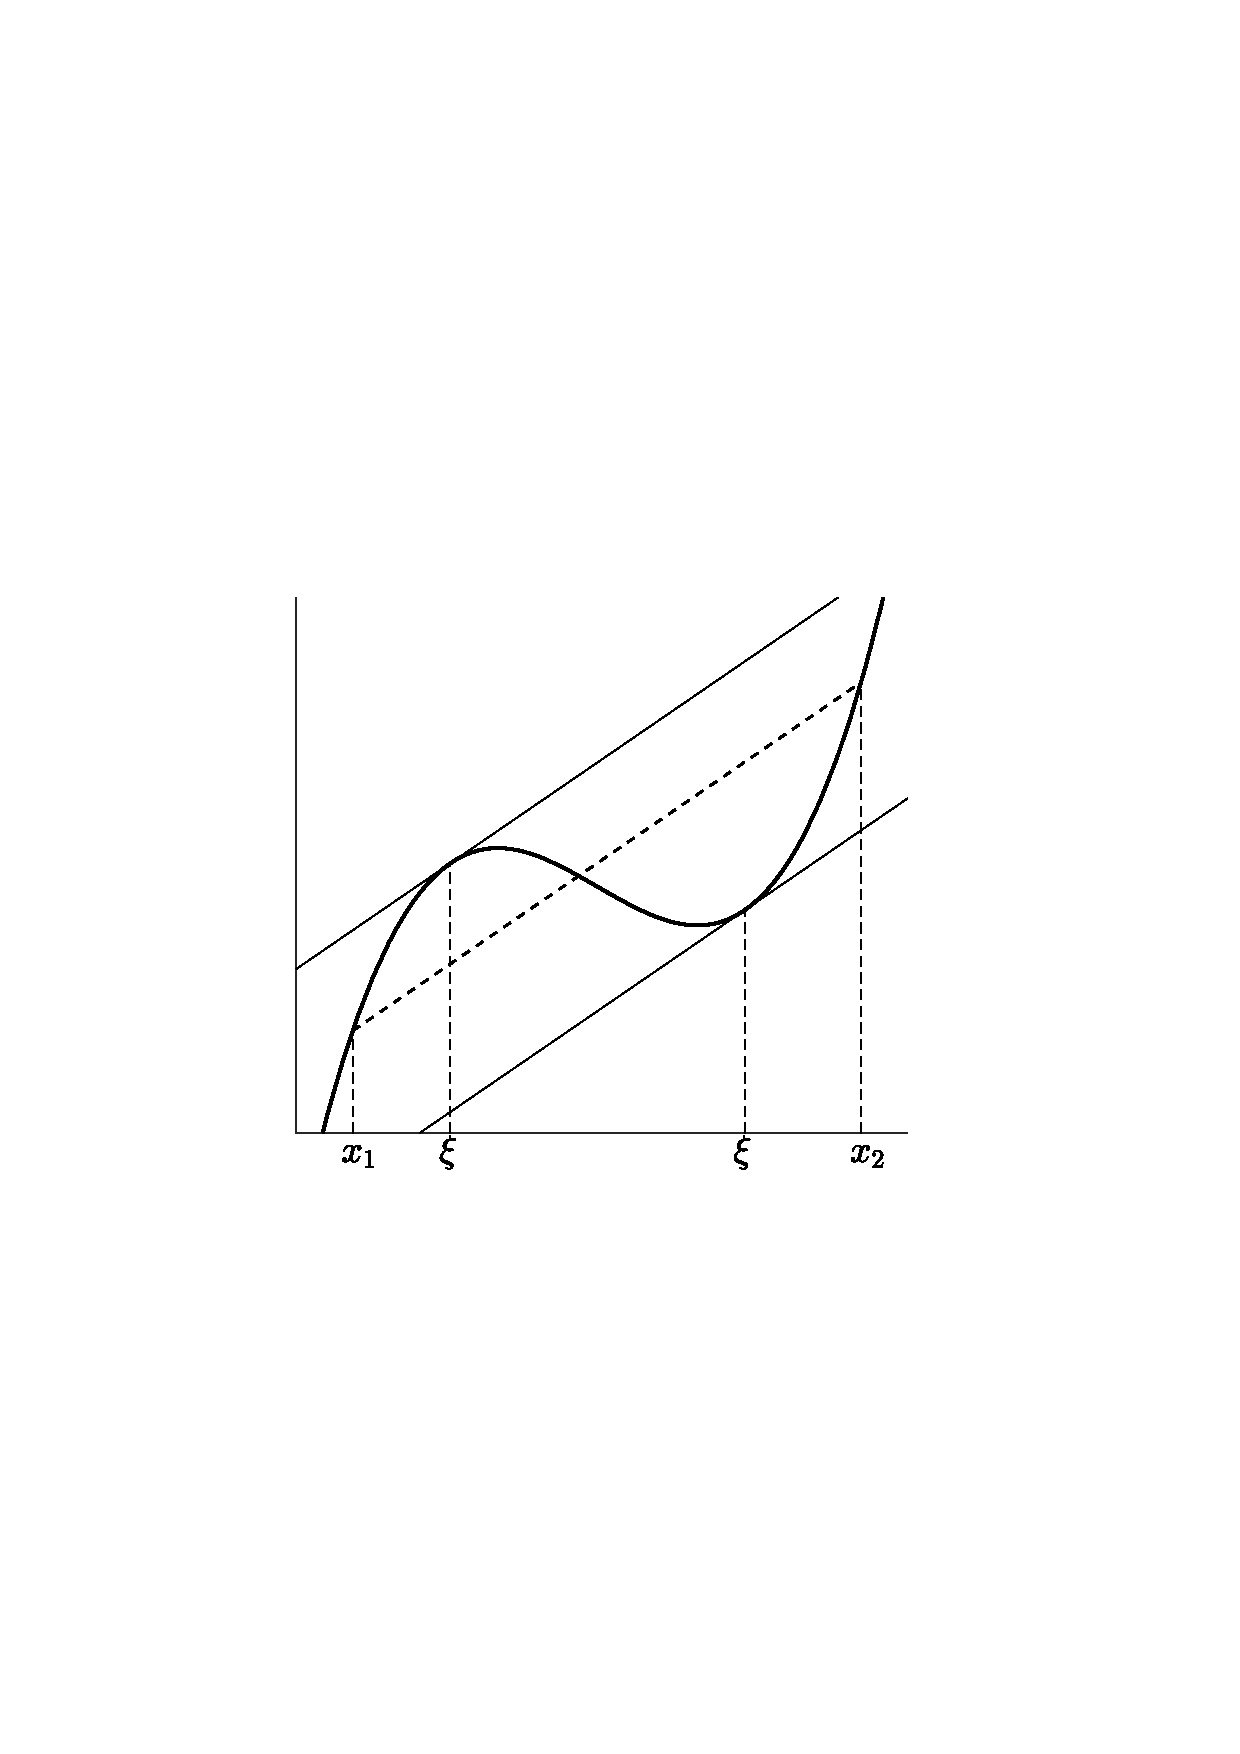
\includegraphics[width=0.4\linewidth]{拉格朗日中值定理主图}
\end{figure}

反比例函数$ y=\dfrac{1}{x} $在区间$ [-1,1] $内不连续($ x=0 $处不连续),
所以该函数不存在与过$ (-1,-1),(1,1) $两点的割线斜率相同的切线。
绝对值函数$ y=|x| $在\textbf{R}上连续,但在$ x=0 $处不可导,
所以该函数不存在与过$ (-1,1),(1,1) $两点的割线斜率相同的切线。

下面来分析为什么函数的凹凸性与二阶导数的正负有关。记
$ u=\lambda x_1+(1-\lambda)x_2,\ \lambda\in(0,1) $,假设$ \lambda f(x_1)+
(1-\lambda)f(x_2) >f(\lambda x_1+(1-\lambda)x_2)=f(u) $,那么:
\begin{align*}
    \lambda f(x_1)+(1-\lambda)f(x_2) & >\left[ \lambda +(1-\lambda) \right]  f(u) \\
    (1-\lambda)\left[ f(x_2)-f(u)\right] &>\lambda \left[f(u)- f(x_1) \right]   \\
    \dfrac{f(x_2)-f(u)}{ \lambda } &> \dfrac{f(u) - f(x_1)}{1-\lambda}  \\
    \dfrac{f(x_2)-f(u)}{ \lambda (x_2-x_1)} &> \dfrac{f(u) - f(x_1)}{(1-\lambda)(x_2-x_1)} 
\end{align*}
因为
\begin{align*}
    u-x_1 =&\lambda x_1+(1-\lambda)x_2-x_1=(1- \lambda)(x_2-x_1) \\
    x_2-u =&x_2-\lambda x_1-(1-\lambda)x_2=\lambda (x_2-x_1) 
\end{align*}
所以:
\begin{align}\label{GeXianXieLv}
    \dfrac{f(x_2)-f(u)}{ x_2-u} > \dfrac{f(u) - f(x_1)}{u-x_1} 
\end{align}
(\ref{GeXianXieLv})式含义很明确,代表两条割线斜率的大小关系。
根据拉格朗日中值定理,存在$ \xi_1 \in (x_1,u),\xi_2 \in (u,x_2) $,使得
$ f'(\xi_1)=\dfrac{f(u) - f(x_1)}{u-x_1}, \ f'(\xi_2)=\dfrac{f(x_2)-f(u)}{ x_2-u} $,
于是(\ref{GeXianXieLv})式成为$ f'(\xi_2) > f'(\xi_1) $,由于$ x_1,x_2 $的任意性(并且两者可以任意接近),
$ \xi_1,\xi_2\ (\xi_1<\xi_2) $也具有一定的任意性。所以,$ f'(\xi_2) > f'(\xi_1) $
意味着$ f'(x) $单调递增,$ f''(x) > 0 $. \\
\\
\textbf{三角函数} \\
$ 0<x_1<\xi<x_2<\pi$,\ $ (\sin x)'=\cos x $在$ [0,\pi] $上递减,于是有
\begin{align*}
    \cos x_1>\dfrac{\sin x_2 - \sin x_1}{x_2 -x_1}=\cos \xi>\cos x_2 
\end{align*}
如果不使用中值定理,要证明上面的不等式成立,可以固定$ x_1 $,然后对$ x_2 $求导。
判断导数的正负号时,可以只看分子,不看分母,因为分母是一个平方式。\\
\\
\textbf{指数函数和对数函数} \\
$ (\e^x)'=\e^x $在\textbf{R}上递增;$ (\ln x)'=\dfrac{1}{x} $在$ (0,+\infty) $上递减。\\
$ u\neq 0 $时,$ \e^u>1+u $,令$ u=x_2-x_1>0 $,则$ \e^{x_2-x_1}-1>x_2-x_1 $,
$ \dfrac{\e^{x_2-x_1}-1}{x_2-x_1}>1 $,两边同乘$ \e^{x_1} $便得到下列不等式的左半部分。
利用$ \e^{-u}>1-u $,右半部分可类似证明。
\begin{align*}
    \e^{x_1}<\dfrac{\e^{x_2}-\e^{x_1}}{x_2-x_1} = \e^{\xi} <\e^{x_2} 	
\end{align*}
因为$ u\neq 1 $时,$ \ln u<u-1 $,令$ u=\dfrac{x_2}{x_1},\ \ln\dfrac{x_2}{x_1}< \dfrac{x_2}{x_1}-1 $,这
就是下式的左半部分。利用$ \ln \dfrac{1}{u}<\dfrac{1}{u}-1 $,右半部分可类似证明。
\begin{align*}
    \dfrac{1}{x_1}>\dfrac{\ln x_2-\ln x_1}{x_2-x_1}=\dfrac{1}{\xi} >\dfrac{1}{x_2}
\end{align*}
$ \e^x $与$ \ln x $互为反函数,两者的图像关于直线$ y=x $对称,请结合图像思考上面的不等式。\\
\\
\textbf{幂函数} \\
$ (x^{\alpha})'=\alpha x^{\alpha-1} $,当$ \alpha > 1 $时递增。
以下均认为 $ 0<x_1<\xi<x_2 $ \\
若$ m,n $均为整数且互质,
\begin{align*}
    \dfrac{x_2^{\frac{n}{m}}-x_1^{\frac{n}{m}}}{x_2-x_1} =&\dfrac{\left(x_2^{\frac{1}{m}} 
        -x_1^{\frac{1}{m}}\right) \left( x_2^{\frac{n-1}{m}}+x_2^{\frac{n-2}{m}}x_1^{\frac{1}{m}}
        + \cdots +x_2^{\frac{1}{m}}x_1^{\frac{n-2}{m}}+x_1^{\frac{n-1}{m}}\right) }{\left(
        x_2^{\frac{1}{m}} -x_1^{\frac{1}{m}} \right) \left(x_2^{\frac{m-1}{m}}+x_2^{\frac{m-2}{m}}
        x_1^{\frac{1}{m}}+ \cdots +x_2^{\frac{1}{m}}x_1^{\frac{m-2}{m}}+x_1^{\frac{m-1}{m}} \right) } \\
    =&\dfrac{x_2^{\frac{n-1}{m}}+x_2^{\frac{n-2}{m}}x_1^{\frac{1}{m}}+ \cdots 
        +x_2^{\frac{1}{m}}x_1^{\frac{n-2}{m}}+x_1^{\frac{n-1}{m}} }{x_2^{\frac{m-1}{m}}
        +x_2^{\frac{m-2}{m}}x_1^{\frac{1}{m}}+\cdots +x_2^{\frac{1}{m}}x_1^{\frac{m-2}{m}}
        +x_1^{\frac{m-1}{m}} }
\end{align*}
$ m=1,n $为大于1的正整数时,
\begin{align*}
    nx_1^{n-1}<\dfrac{x_2^n-x_1^n}{x_2-x_1}=x_2^{n-1}+x_2^{n-2}x_1+\cdots +
    x_2x_1^{n-1}+x_1^{n-1}=n\xi^{n-1} < nx_2^{n-1}
\end{align*}
$ \dfrac{n}{m}=\dfrac{1}{2} $时,
\begin{align*}
    \dfrac{1}{2\sqrt{x_1}}>\dfrac{\sqrt{x_2}-\sqrt{x_1}}{x_2-x_1}=\dfrac{1}{\sqrt{x_2}+\sqrt{x_1}}
    =\dfrac{1}{2\sqrt{\xi}}>\dfrac{1}{2\sqrt{x_2}}
\end{align*} 
$ \dfrac{n}{m}=\dfrac{3}{2} $时,
\begin{align*}
    \dfrac{3}{2}\sqrt{x_1}< \dfrac{x_2^{3/2}-x_1^{3/2}}{x_2-x_1}=
    \dfrac{(\sqrt{x_2}-\sqrt{x_1})(x_2+\sqrt{x_2x_1}+x_1)}{x_2-x_1}=
    \dfrac{x_2+\sqrt{x_2x_1}+x_1}{\sqrt{x_2}+\sqrt{x_1}} < \dfrac{3}{2}\sqrt{x_2}
\end{align*}
容易验证:$ \dfrac{3}{2}\sqrt{x_1}(\sqrt{x_2}+\sqrt{x_1})<x_2+\sqrt{x_2x_1}+x_1
<\dfrac{3}{2}\sqrt{x_2}(\sqrt{x_2}+\sqrt{x_1}) $.\\
$ \dfrac{n}{m}=-1 $时,
\begin{align*}
    -\dfrac{1}{x_1^2}<\dfrac{\frac{1}{x_2}-\frac{1}{x_1}}{x_2-x_1}=-\dfrac{1}{x_1x_2}<
    -\dfrac{1}{x_2^2}
\end{align*}

\item 狄利克雷逼近定理:对任意实数 $\alpha$,正整数 $N>1$,
都存在整数 $p$ 和 $q$,其中 $1\leq q\leq N$,使得
$\left|\alpha-\dfrac{p}{q}\right|<\dfrac{1}{qN}$成立。  \\
\textbf{证}\ 
定义$\{x\}=x-\lfloor x\rfloor$,其中 $ \lfloor x\rfloor $ 
是向下取整函数(不超过$x$的最大整数),
比如$ \lfloor 2.1\rfloor=\lfloor 2.7\rfloor=2 $,
$\lfloor -4.2\rfloor=\lfloor -4.9\rfloor=-5 $. 
显然有$ 0\leq \{x\}<1 $.  \\
现在考虑 $\{\alpha\},\{2\alpha\},\cdots,\{(N+1)\alpha\}$
共$N+1$个落在区间$[0,1)$内的小数。
现在把区间$[0,1)$等分成$N$个子区间,如下
\begin{gather*}
    \left[0,\frac{1}{N}\right),
    \left[\frac{2}{N},\frac{3}{N}\right),
    \left[\frac{3}{N},\frac{4}{N}\right),\cdots,
    \left[\frac{N-1}{N},1\right)
\end{gather*}
根据抽屉原理,必然有两个不同的正整数$i,j$(不妨设$i<j$)满足 $\{i\alpha\},\{j\alpha\}$ 同时落在某个子区间内。
即$|\{i\alpha\}-\{j\alpha\}|<\dfrac{1}{N}$,
又因为$1\leq i<j\leq N+1$,那么有$1\leq j-i\leq N$.
再利用$\{x\}=x-\lfloor x\rfloor$,得到
\begin{gather*}
    \left|\{j\alpha\}-\{i\alpha\}\right|=\left|
    (j-i)\alpha-(\lfloor j\alpha\rfloor
    -\lfloor i\alpha\rfloor)\right|<\frac{1}{N}
\end{gather*}
令$q=j-i,\ p=\lfloor j\alpha\rfloor-\lfloor i\alpha\rfloor$,显然 $1\leq q\leq N$. 
将$p,q$代入上式,有 $|q\alpha-p|<\dfrac{1}{N}$,
也就是 $\left|\alpha-\dfrac{p}{q}\right|<\dfrac{1}{qN}$,证毕。

\item $^*$ 刘维尔(Liouville)逼近定理\footnote{2017年天津高考考察了刘维尔逼近定理。}:设$ f(x)=a_nx^n+a_{n-1}x^{n-1}+
\cdots+a_1x+a_0 $,其中$ a_n\neq 0,\ a_j\in \textbf{Z}\ 
(0\leq j\leq n) $. 又设$ x_0 $是$ f(x) $的零点,且$ x_0 $
不是有理数,那么存在实数$ A>0 $,使得对任意$ p\in \textbf{Z},\ 
q\in \textbf{N}^+ $,都有$ \left|x_0-\dfrac{p}{q}\right|>
\dfrac{A}{q^n} $.\\
\textbf{方法一}\ 存在充分接近$ x_0 $的有理数$ \dfrac{p}{q} $,
使得$ f\left(\dfrac{p}{q}\right)\neq 0 $,
\begin{align*}
    \left|f\left(\dfrac{p}{q}\right)\right|=\left|\sum_{j=0}^{n}a_{j}\cdot \left(\dfrac{p}{q}\right)^{j}\right|=\dfrac{\left|\sum\limits_{j=0}^{n}a_{j}\cdot p^{j}\cdot q^{n-j}\right|}{q^{n}}\geq \dfrac{1}{q^{n}}
\end{align*}
最后一个不等号是因为$ \left|\sum\limits_{j=0}^{n}a_{j}\cdot p^{j}
\cdot q^{n-j}\right| $为正整数,那么必然大于等于1.
然后分两种情况讨论: \\
\mycircled{1} $ \left|x_0-\dfrac{p}{q}\right|\geq 1 $ ,
此时显然有:$ \forall q\geq 1:\left|x_0-\dfrac{p}{q}\right|\geq 1\geq \dfrac{1}{q^{n}} $ ,任取 $ A_{1}<1 $ 即可满足定理的要求。\\
\mycircled{2} $ \left|x_0-\dfrac{p}{q}\right|<1 $,
由 $ f(x_0)=\sum\limits_{j=0}^{n}a_{j}\cdot x_0^{j}=0 $ 可得
\begin{align*}
    -f\left(\dfrac{p}{q}\right)=f(x_0)-f\left(\dfrac{p}{q}\right)
    &=\sum_{j=1}^{n}a_{j}\cdot\left[x_0^{j}-\left(\dfrac{p}{q}
    \right)^{j}\right] \\
    &=\left(x_0-\dfrac{p}{q}\right)\cdot 
    \sum_{j=1}^{n}a_{j}\cdot \left[\sum_{k=1}^{j}x_0^{j-k}\cdot
    \left(\dfrac{p}{q}\right)^{k-1}\right]
\end{align*}
以上过程运用了恒等式$ x^{n}-y^{n}=(x-y)(x^{n-1}+x^{n-2}y+\cdots+y^{n-1}) $. 由上式可得: 
\begin{align}\label{刘维尔定理1}
    \dfrac{\left|f\left(\dfrac{p}{q}\right)\right|}{\left|x_0-\dfrac{p}{q}\right|}=\left|\sum_{j=1}^{n}a_{j}\cdot \left[\sum_{k=1}^{j}x_0^{j-k}\cdot \left(\dfrac{p}{q}\right)^{k-1}\right]\right|\leq \sum_{j=1}^{n}\left|a_{j}\right|\cdot \left[\sum_{k=1}^{j}|x_0|^{j-k}\cdot \left|\dfrac{p}{q}\right|^{k-1}\right]
\end{align}
由 $ \left|\dfrac{p}{q}\right|-|x_0|\leq \left|x_0-\dfrac{p}{q}\right|<1 $ 可得:
$ \left|\dfrac{p}{q}\right|<|x_0|+1 $ ,代入上式得到
\begin{align*}
    \dfrac{\left|f\left(\dfrac{p}{q}\right)\right|}{\left|x_0-\dfrac{p}{q}\right|} 
    &\leq \sum_{j=1}^{n}\left|a_{j}\right|\cdot \left[\sum_{k=1}^{j}|x_0|^{j-k}\cdot \left|\dfrac{p}{q}\right|^{k-1}\right]\\ &<\sum_{j=1}^{n}\left|a_{j}\right|\cdot \left[\sum_{k=1}^{j}|x_0|^{j-k}\cdot (|x_0|+1)^{k-1}\right]=m(x_0)>0
\end{align*}
从而 $ \left|x_0-\dfrac{p}{q}\right|>\dfrac{\left|f\left(\frac{p}{q}\right)\right|}{m(x_0)}\geq \dfrac{\frac{1}{m(x_0)}}{q^{n}} $ ,令 $ A_{2}\leq \dfrac{1}{m(x_0)} $ ,即可满足定理要求。\\
综合以上,令$ A=\min\left\{A_{1},A_{2}\right\} $ ,即成立 $ \forall p\in\textbf{Z},\ q\in\textbf{N}^{+} $,有$ \left|x_0-\dfrac{p}{q}\right|>\dfrac{A}{q^{n}} $. 证毕。\\
\textbf{方法二}\ $ \left|x_0-\dfrac{p}{q}\right|\geq 1 $的情况同上,只考虑
$ \left|x_0-\dfrac{p}{q}\right|<1 $,应用拉格朗日中值定理,
存在$ \xi $介于$ x_0 $与$ \dfrac{p}{q} $之间,使得
\begin{gather*}
    |f'(\xi)|=\dfrac{\left|f(x_0)-f\left(\dfrac{p}{q}\right)
        \right|}{\left|x_0 -\dfrac{p}{q}\right|}=
    \dfrac{\left|f\left(\dfrac{p}{q}\right)
        \right|}{\left|x_0-\dfrac{p}{q}\right|}
\end{gather*}
由多项式函数的连续性,$ |f'(\xi)| $必然不超过$ |f'(x)| $在区间$ (x_0-1,x_0+1) $
上的最大值$ M\ (M>0) $,所以
\begin{gather*}
    \left|x_0-\dfrac{p}{q}\right|=
    \dfrac{\left|f\left(\dfrac{p}{q}\right)\right|}{\left|f'(\xi)\right|}\geq 
    \dfrac{\left|f\left(\dfrac{p}{q}\right)\right|}{M}=
    \dfrac{\left|\sum\limits_{j=0}^{n}a_{j}\cdot p^{j}\cdot q^{n-j}\right|}{Mq^{n}}\geq \dfrac{1}{Mq^{n}}
\end{gather*}
取$ A_1<1,\ A_2\leq \dfrac{1}{M} $ ,$ A=\min\left\{A_{1},A_{2}\right\} $ 即可。证毕。

下面以$ f(x)=x^2-2,\ x_0=\sqrt{2} $为例,用具体数字感受一下刘维尔定理。
$ f'(x)=2x $,当$ x\in(\sqrt{2}-1,\sqrt{2}+1) $时,
$ |f'(x)|<2(\sqrt{2}+1)<5 $,
\begin{align*}
    & \left|\sqrt{2} -\dfrac{3}{2}\right|=0.085786\cdots >\dfrac{1}{5\cdot 2^2}=0.05  \\
    & \left|\sqrt{2} -\dfrac{7}{5}\right|=0.014213\cdots >\dfrac{1}{5\cdot 5^2}=0.008  \\
    & \left|\sqrt{2} -\dfrac{17}{12}\right|=0.002453\cdots >\dfrac{1}{5\cdot 12^2}=0.001388\cdots  \\
    & \left|\sqrt{2} -\dfrac{41}{29}\right|=0.000420\cdots >\dfrac{1}{5\cdot 29^2}=0.000237\cdots  \\
    & \left|\sqrt{2} -\dfrac{99}{70}\right|=0.000072\cdots >\dfrac{1}{5\cdot 70^2}=0.000040\cdots 
\end{align*}
\textbf{注}:$ \dfrac{3}{2},\ \dfrac{7}{5},\ \dfrac{17}{12} $等分数是用MATLAB的rats函数找到的,
语法为rats(sqrt(2),3),后面的3可以改成更大的正整数,改得越大,得到的分数越接近$ \sqrt{2} $.
$ \dfrac{3}{2} $是所有分母为$ 2 $的分数中,最接近$ \sqrt{2} $的,其余分数类似。
感兴趣的还以以$ \sqrt[3]{2} $为例进行计算,逼近$ \sqrt[3]{2} $的分数有
$ \dfrac{5}{4},\ \dfrac{34}{27},\ \dfrac{63}{50}\cdots $. 

\end{itemize}

\section{拉格朗日反演$ ^* $}
\begin{itemize}[leftmargin=\inteval{\myitemleftmargin}pt,itemsep=
   \inteval{\myitemitempsep}pt,topsep=\inteval{\myitemtopsep}pt]
\item 除了少数十分简单的函数,绝大多数函数都无法写出其反函数的显式表达式。
比如$ y=xe^x $的反函数为$ x=y\e^{y}=W(x)\e^{W(x)} $,无法写出$ W(x) $关于
$ x $的显式表达式,$ W(x) $被称为Lambert W函数\footnote{
可查阅Wolfram MathWorld上Lambert W-Function词条。}。$ y=x+\ln x $的反函数为
$ x=y+\ln y $,这个反函数被称为Wright Omega函数,也写不出显式表达式。
但我们可以使用幂级数来研究这些反函数,计算一个函数的反函数的幂级数的方法,
被称为拉格朗日反演(Lagrange inversion),具体如下:

设$ y=f(x) $经过点$ (x_0,f(x_0)) $,且$ f'(x_0)\neq 0 $,那么其反函数经过点
$ (f(x_0),x_0) $,反函数在$ x=f(x_0) $处的泰勒级数(幂级数)为:
\begin{gather}\label{拉格朗日反演公式}
    y=f(x_0)+\sum_{k=1}^{\infty}\left\{\lim_{x\to x_0}\dfrac{\d^{k-1}}{\d x^{k-1}}
    \left[\dfrac{x-x_0}{f(x)-f(x_0)}\right]^k\right\}\cdot 
    \dfrac{[x-f(x_0)]^k}{k!}
\end{gather}

\item 三个数学软件求反函数的语法 
\begin{table}[!htbp]
%\vspace{-2mm}
\centering
\begin{tabular}{|r|l|}
    \hline
    MATLAB & syms x; finverse(x*exp(x)) \\ \hline
    Maple & with(MTM): finverse(x*exp(x)) \\ \hline
    Mathematica & InverseFunction[x*Exp(x)] \\ \hline
\end{tabular}
%\vspace{-3mm}
\end{table} \\

\begin{figure}[!htbp]
    \centering
    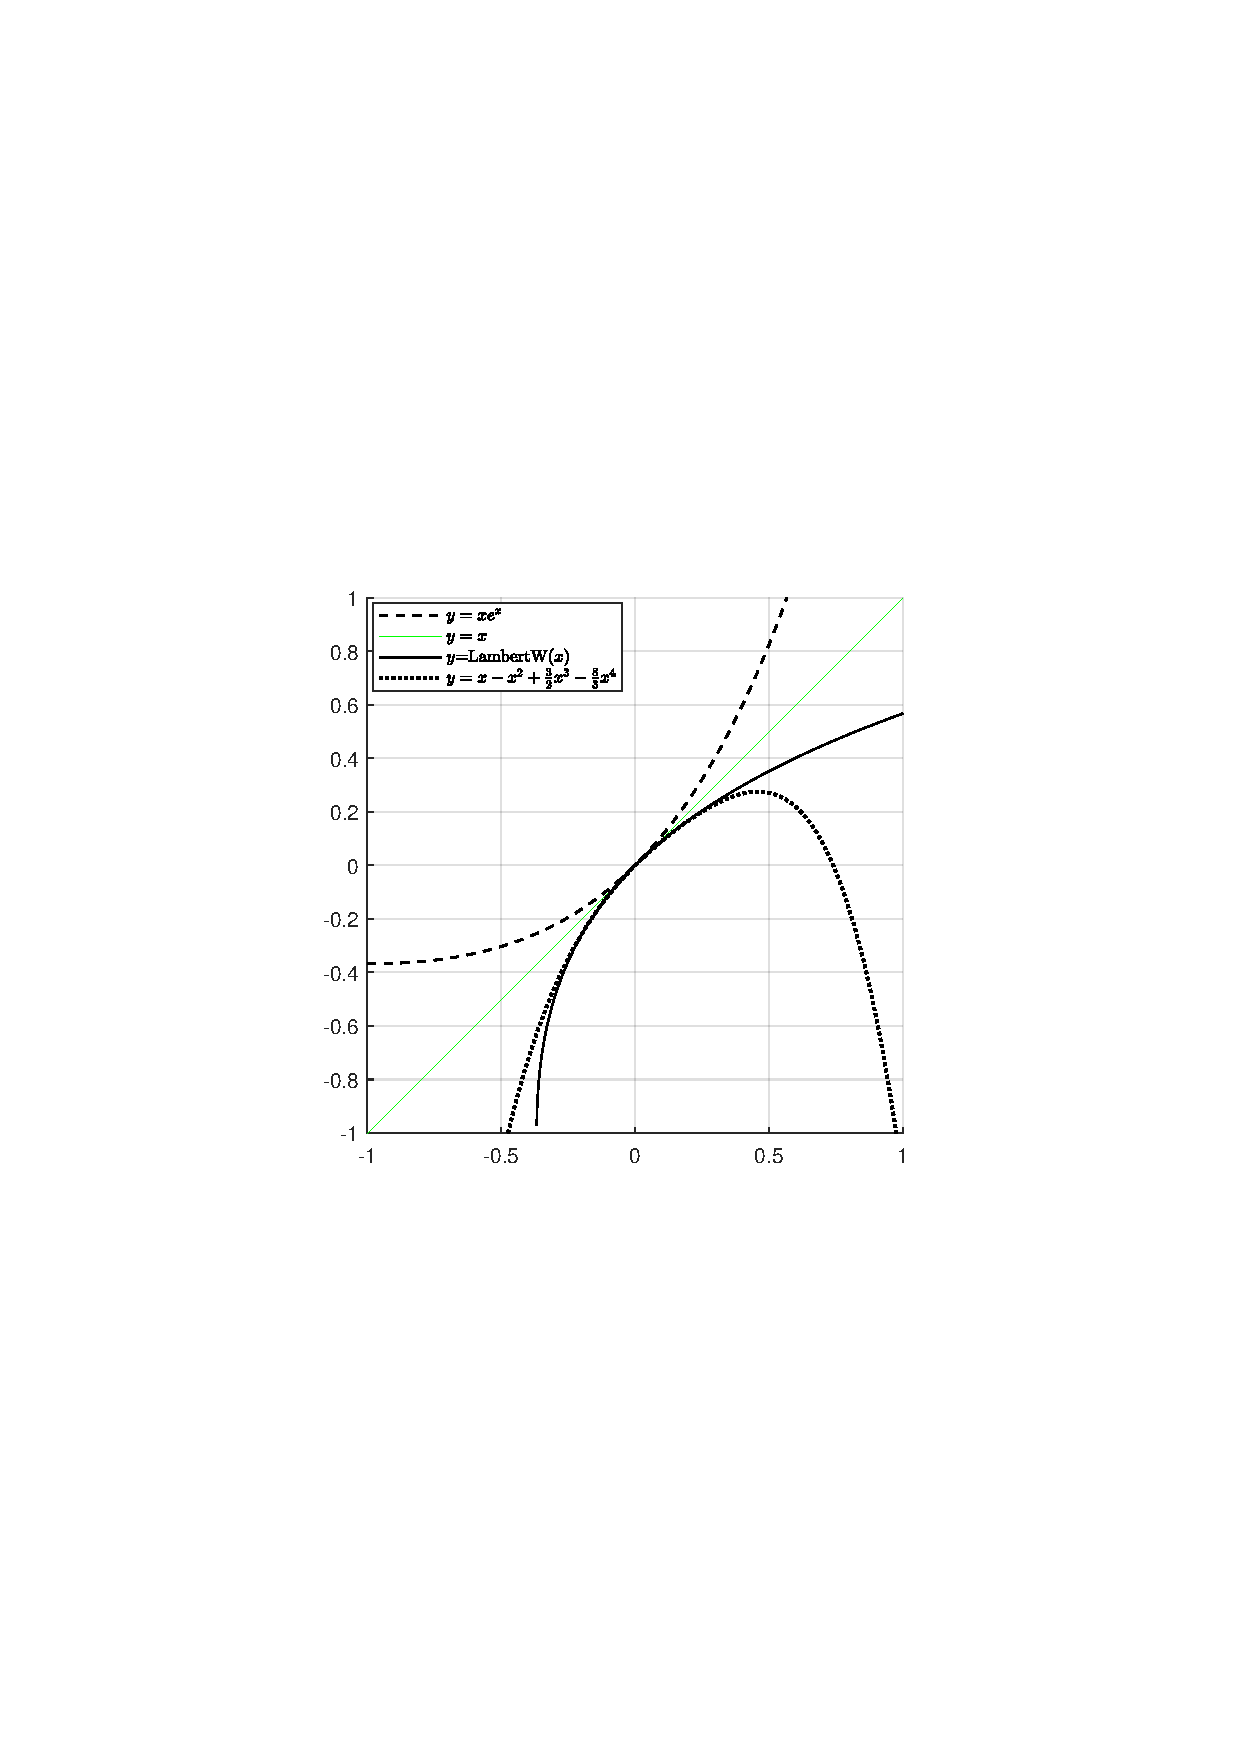
\includegraphics[width=0.5\linewidth]{拉格朗日反演-LamberW}
\end{figure}

% LagrangeInversion.m
\item 令$ f(x)=xe^x $,取$ x_0=0 $,则$ f(x_0)=0 $.
Lambert W函数在$ x=f(x_0)=0 $处的幂级数为:
\begin{gather}\label{LambertW拉格朗日反演x=0}
    W(x)=\sum_{k=1}^{\infty}(-k)^{k-1}\cdot \dfrac{x^k}{k!}
    =x-x^2+\dfrac{3}{2}x^3-\dfrac{8}{3}x^4+\cdots 
\end{gather}
在MATLAB中可用语句taylor(finverse(x*exp(x)),'expansionPoint',0,'order',5)
获得以上结果。取$ x_0=0.5671432904\cdots $,则$ f(x_0)=1 $,
Lambert W函数在$ x=f(x_0)=1 $处的幂级数为:
\begin{gather}\label{LambertW拉格朗日反演x=1}
    W(x)=0.0298074 + 0.803503x - 0.379452x^2 + 0.135843x^3 - 0.022557x^4+\cdots
\end{gather}

\item 令$ f(x)=x+\ln x $,取$ x_0=0.5671432904\cdots $(其实就是$ W(1) $),
则$ f(x_0)=0 $,Wright Omega函数在$ x=f(x_0)=0 $处的幂级数为:
\begin{gather}\label{x+lnx拉格朗日反演x=0}
    0.567143 + 0.361896x + 0.073677x^2 - 0.001342x^3 - 0.001636x^4+\cdots
\end{gather}
取$ x_0=1 $,则$ f(x_0)=1 $,Wright Omega函数在$ x=f(x_0)=1 $处的幂级数为:
\begin{gather}\label{x+lnx拉格朗日反演x=1}
    \dfrac{581}{1024}+\dfrac{277x}{768}+\dfrac{39x^2}{512}
    -\dfrac{x^3}{256}-\dfrac{x^4}{3072}+\cdots
\end{gather}

\item 拉格朗日反演要求$ f'(x_0)\neq 0 $,这是因为原函数上切线斜率为0的点对应反函数上切线斜率为无穷大的点,在前面的泰勒级数一节提到过,切线斜率为无穷大的点,是不存在泰勒级数的(正整数次幂函数在自变量为有限值的情况下,切线斜率无法达到无穷大)。

% pade_approximation.m
\item 很多网上流传的难度较高(通常高于高考难度)的极值点偏移问题,就是以拉格朗日反演为背景。设$ f(x) $存在极值点$ (x_0,f(x_0)) $,则$ f'(x_0)=0 $,按照上面的讨论,不能直接进行拉格朗日反演,可改用$ \sqrt{f(x)-f(x_0)} $(对于极小值点)或$ \sqrt{f(x_0)-f(x)} $(对于极大值点)进行反演
\footnote{参见https://zhuanlan.zhihu.com/p/367058597}。再设$ x_1<x_0<x_2 $,且$ f(x_1)=f(x_2)=m $,则当$ |m-f(x_0)| $比较小时,有
\begin{gather}\label{极值点附近两根之和的估计}
    x_1+x_2\approx 2x_0-\dfrac{2f'''(x_0)}{3[f''(x_0)]^2}[m-f(x_0)]
\end{gather} 

\renewcommand\arraystretch{1.26}
\begin{table}[!htbp]
%\vspace{-2mm}
\centering
\begin{tabular}{|c|l|c|c|c|}
\hline
$ f(x) $ & 极值点 & $ x_1+x_2\approx $ & Pade $ R_{2,1}(x) $ & Pade $ R_{1,2}(x) $ \\ \hline
$ \frac{x}{\ln x} $& 极小$ (\e,\e) $ & $ 2\e+\frac{10}{3}(m-\e) $ &  $ \frac{3x^2+4\e x-\e^2}{10x-4\e}\ \Cup $ & $ \frac{2\e^{2}(-5x+2\e)}{3x^2-16\e x+7\e^2}\ \Cup $  \\ \hline
$ \frac{\ln x}{x} $&  极大$ (\e,\frac{1}{\e}) $ & $ 2\e+\frac{10\e^2}{3}(\e-m) $ & $ \frac{-3x^2+16\e x-7\e^2}{(10x-4\e)\e^2}\ \Cap  $ & $ \frac{10x-4\e}{3x^2+4\e x-\e^2}\ \Cap  $  \\ \hline
$ x\ln x $ & 极小$ (\frac{1}{\e},-\frac{1}{\e}) $ & $ \frac{2}{\e}+\frac{2}{3}(m+\frac{1}{\e}) $ & $ \frac{3\e^2x^2-8\e x-1}{(2\e x+4)\e}\ \Cup $ & $ \frac{2(\e +2)}{(-3\e^2x^2+4\e x-7)\e}\ \Cup $  \\ \hline
$ x\e^x $ & 极小$ (-1,-\frac{1}{\e}) $ & $ -2-\frac{4\e}{3}(m+\frac{1}{\e}) $ & $ \frac{-3x^2-10x-1}{(4x-2)\e}\ \Cup $ & $ \frac{4x-2}{(3x^2+2x+5)\e}\ \Cup $  \\ \hline
$ \frac{x}{\e^x} $ & 极大$ (1,\frac{1}{\e}) $ & $ 2+\frac{4\e}{3}(\frac{1}{\e}-m) $ & $ \frac{-3x^2+10x-1}{(4x+2)\e}\ \Cap $ & $ \frac{4x+2}{(3x^2-2x+5)\e}\ \Cap $  \\ \hline
$ \frac{\e^x}{x} $ & 极小$ (1,\e) $ & $ 2+\frac{4}{3\e}(m-\e) $ &  $ \frac{\e(3x^2-2x+5)}{4x+2}\ \Cup $ & $ \frac{(-4x-2)\e}{3x^2-10x+1}\ \Cup $  \\ \hline
$ \e^x-x $ & 极小$ (0,1) $ & $ -\frac{2}{3}(m-1) $ & $ \frac{-3x^2+2x-6}{2x-6}\ \Cup $ & $ \frac{-6+2x}{3x^2+2x-6}\ \Cup $  \\ \hline
$ x-\ln x  $ & 极小$ (1,1) $ & $ 2+\frac{4}{3}(m-1) $ & $ \frac{3x^2-2x+5}{4x+2}\ \Cup $ & $ \frac{-4x-2}{3x^2-10x+1}\ \Cup $ \\ \hline
\end{tabular}
%\vspace{-3mm}
\end{table} 

%\XSolidBrush

上表中的帕德逼近均是在极值点处进行的,有趣的是:$ x^2 $的系数(不考虑正负号)只出现了$ 3,\ 3e,\ 3e^2 $这三种。
如果在极值点的邻域内,$ f(x)-R_{m,n}(x) $不变号,(意思是:极值点左右的小范围内,$ R_{m,n}(x) $始终在$ f(x) $的上方(或下方),两者不发生交叉,用$ \Cup $或$ \Cap $符号表示),那么可以命制$ |x_2-x_1|<\varphi(m) $或$ |x_2-x_1|>\varphi(m) $型的不等式证明题。如果经过极值点后,$  f(x)-R_{m,n}(x) $变号(即两者发生交叉,但上表中没有发生交叉的),那么可以命制$ x_1+x_2<\varphi(m) $或$ x_1+x_2>\varphi(m) $型的不等式证明题。

比如,$ f(x)=\dfrac{x}{\ln x}\leq R_{2,1}(x)=\dfrac{3x^2+4\e x-\e^2}{10x-4\e}\ (x>1) $,属于不交叉型,设$ x_1<x_3<\e<x_4<x_2,\ f(x_1)=R_{2,1}(x_3)=R_{2,1}(x_4)=f(x_2)=m>\e $,那么$ |x_2-x_1|>\underbrace{|x_4-x_3|=\dfrac{2}{3}\sqrt{25m^2-32me+7e^2}}_{\text{两根之差的绝对值为}\frac{\sqrt{\Delta}}{|a|}}=\varphi(m) $. 

又比如$ f(x)=x-\ln x $在$ x=1 $处,如果用$ \dfrac{2(x-1)}{x+1} $来逼近$ \ln x $,进而得到$ x-\ln x \approx x-\dfrac{2(x-1)}{x+1}=\dfrac{x^2-x+2}{x+1}=g(x) $,$ g(x) $属于交叉型,(但其精度也不如不交叉型的$ R_{2,1}(x)=\dfrac{3x^2-2x+5}{4x+2} $).设$ x_3<x_1<1<x_4<x_2,\ g(x_3)=f(x_1)=g(x_4)=f(x_2)=m>1 $,那么$ x_1+x_2>\underbrace{x_3+x_4=m+1}_{\text{两根之和,韦达定理}}=\varphi(m) $. 

\end{itemize}

\section{积分}
\begin{itemize}[leftmargin=\inteval{\myitemleftmargin}pt,itemsep=
   \inteval{\myitemitempsep}pt,topsep=\inteval{\myitemtopsep}pt]

% DingJifenXiFen.m
\item 定积分的几何意义是曲线$ y=f(x) $和$ x $轴、$ x=a $、 $ x=b $
三条直线围成的曲边梯形的面积。在$ x $轴上方的图形的面积认为是正值,在$ x $轴下方的
图形的面积认为是负值。为了计算这个大曲边梯形的面积,可以把区间$ [a,b] $分成一些小区间,
在这些小区间上,做出以小区间内某一点函数值(比如左端点函数值)为高的矩形,这个小矩形的面积
就能近似代替小曲边梯形的面积,所有小矩形面积之和也能近似代替整个大曲边梯形的面积。
随着小区间划分数量越来越多,每个小矩形的宽度都越来越小,所有小矩形面积之和也越来越接近
大曲边梯形的面积。当小区间划分数量趋于无穷大,而每个小矩形宽度都趋于0,那么
所有的小矩形面积之和就等于曲边梯形的真实面积。
\begin{figure}[h]
    \centering
    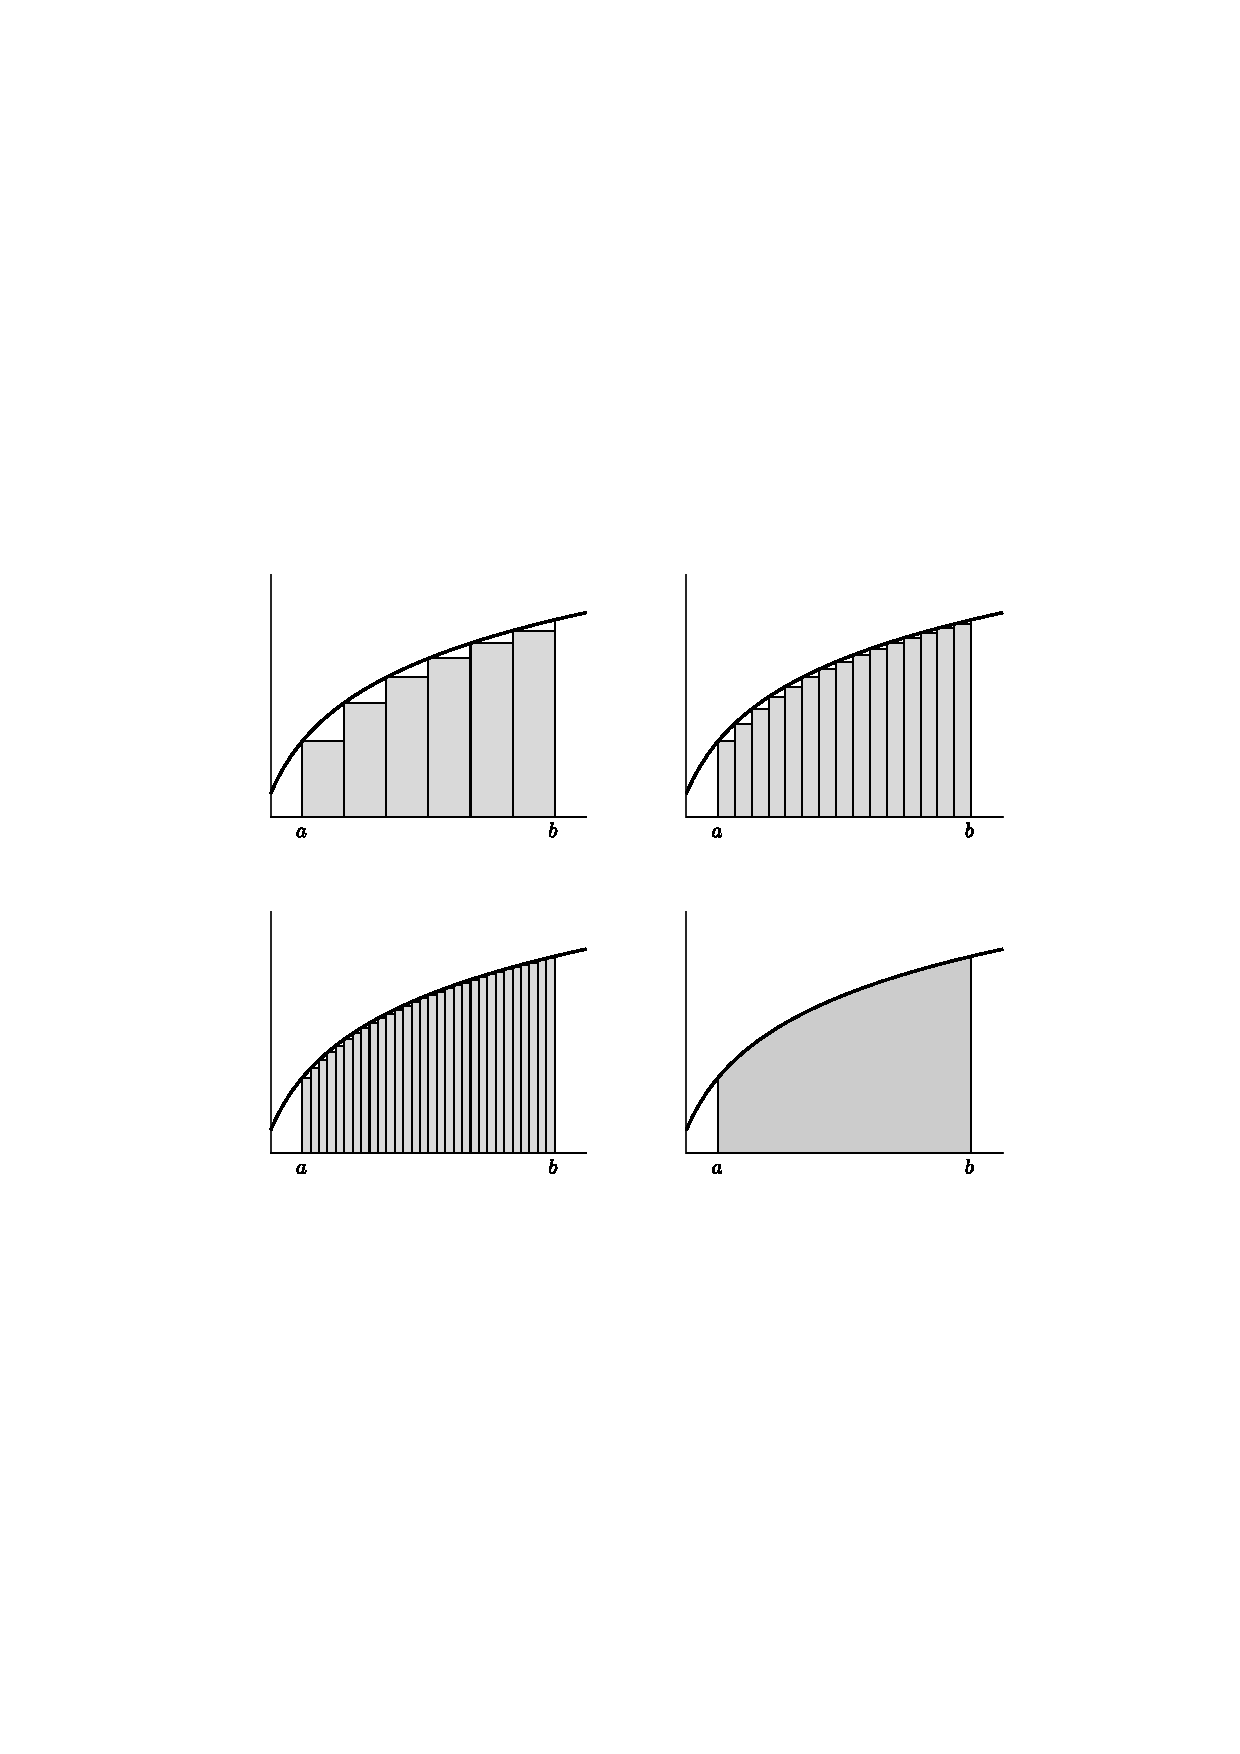
\includegraphics[width=0.7\linewidth]{定积分无限细分}
\end{figure}

% DingJifen_JuXing_TiXing.m
肯定有读者会提出疑问,如果在小区间上不是画矩形,而是画直角梯形,
那算出来的面积不就更加精确吗?
\begin{figure}[h]
    \centering
    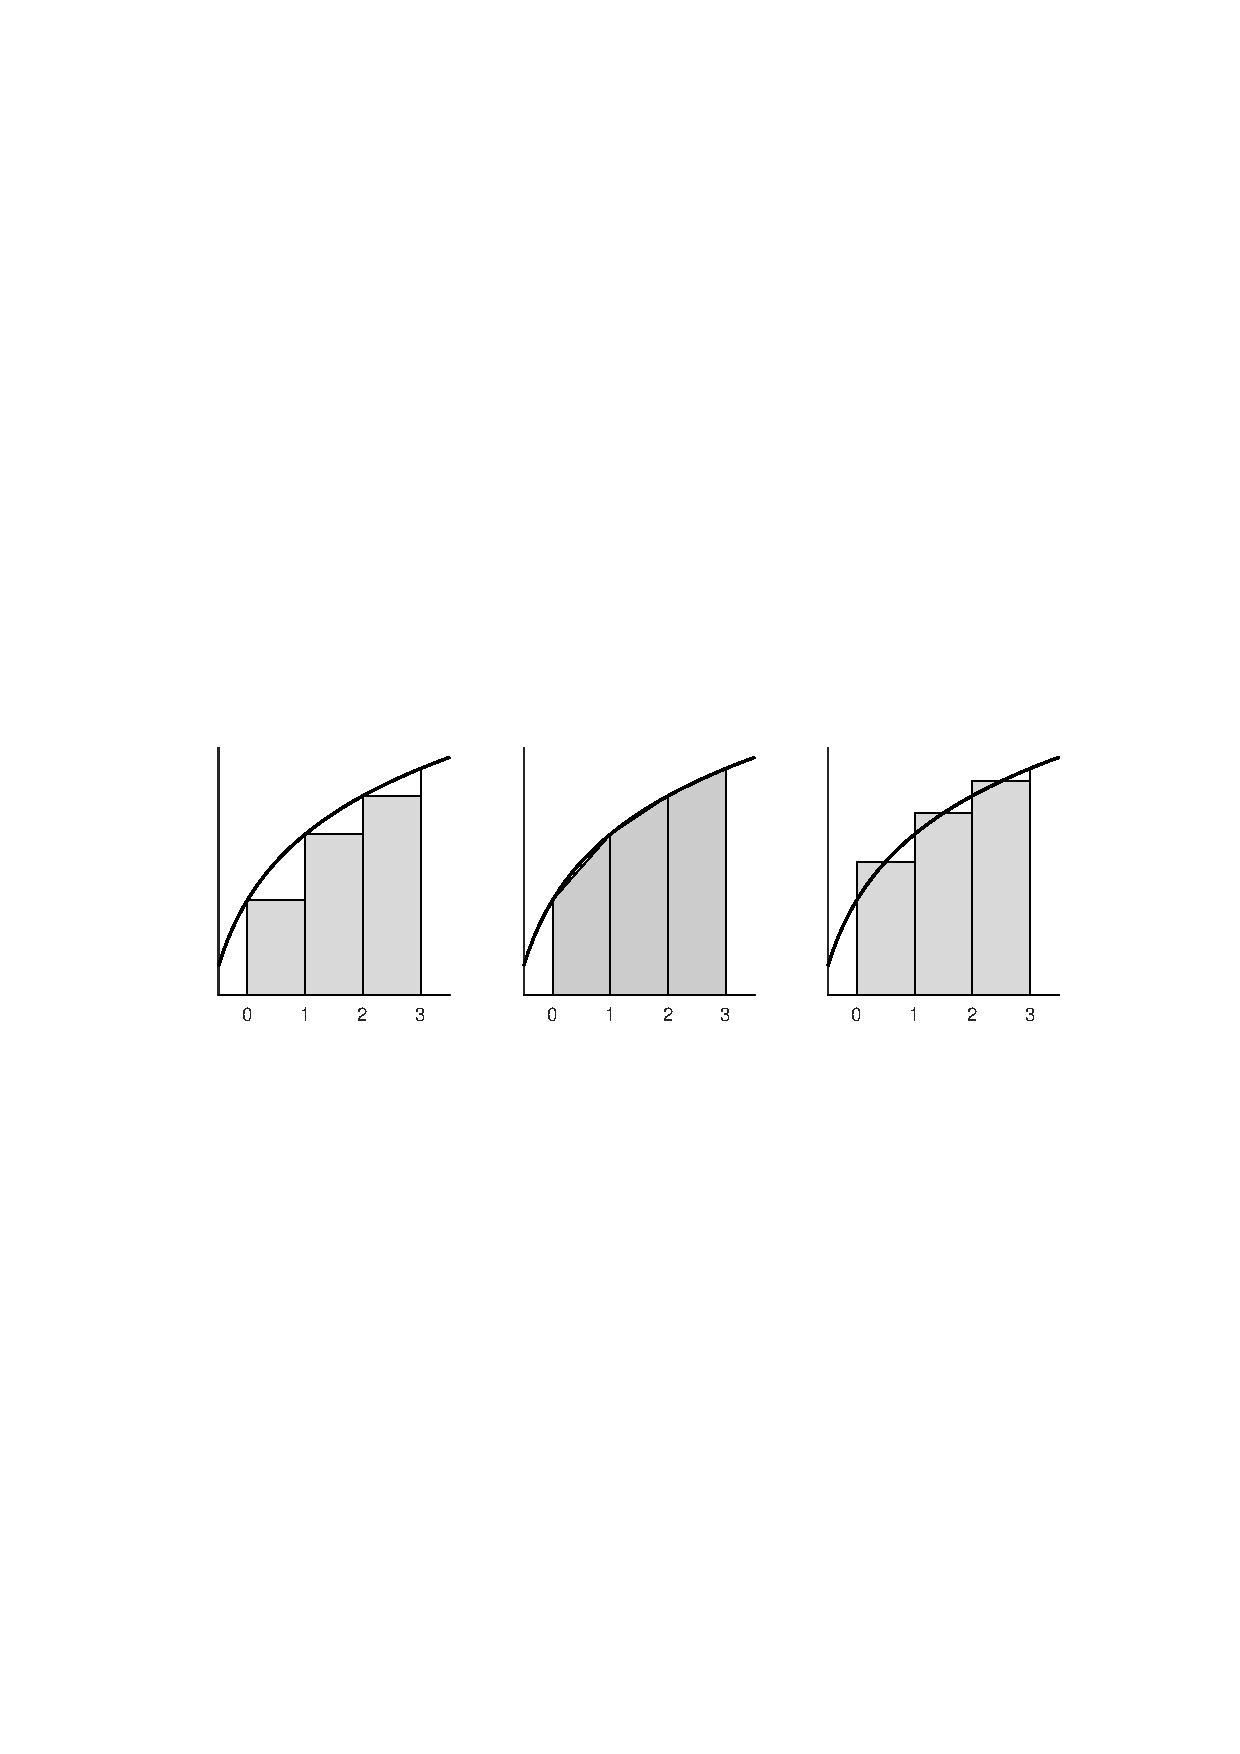
\includegraphics[width=0.6\linewidth]{矩形法与梯形法}
\end{figure}

这种直觉基本正确,以上图为例,假设区间$ [a,b] $为$ [0,3] $,将此区间等分成3份,
按照左图的矩形画法,$ S_{\text{矩}}=f(0)+f(1)+f(2) $,一共使用了3个函数值。
按照中间图的梯形画法,$ S_{\text{梯,4}}= \dfrac{1}{2}[f(0)+f(1)]+\dfrac{1}{2}
[f(1)+f(2)]+\dfrac{1}{2}[f(2)+f(3)]=\dfrac{1}{2}f(0)+f(1)+f(2)+\dfrac{1}{2}f(3) $,
一共使用了4个函数值,比矩形法多用了一个函数值。两种方法的差距为
\begin{gather*}
    S_{\text{梯,4}}-S_{\text{矩}}=\dfrac{1}{2}[f(3)-f(0)]
\end{gather*}
面积差距完全取决于$ f(3) $与$ f(0) $的差距。不过,在比较不同方法优劣的时候,应该要求使用
相同数量的函数值,所以应当比较$ S_{\text{矩}} $与$ S_{\text{梯,3}}=\dfrac{1}{2}
[f(0)+f(1.5)]+\dfrac{1}{2}[f(1.5)+f(3)]=\dfrac{1}{2}f(0)+f(1.5)+\dfrac{1}{2}f(3) $ 
的差距。另外,如右图,仍然画矩形,但是以区间中点函数值为矩形的高,那么$ S_{\text{矩,中}}
=f(0.5)+f(1.5)+f(2.5) $,只使用了3个函数值。当$ f(x) $在区间$ [a,b] $上单调递增时,
右图算法的精度明显高于左图。

以上对求面积的不同方法的精度的讨论,均是在划分的小区间总数有限的情况下进行的。
在用计算机做定积分的时候(计算机只能对有限个数求和,不可能对无穷多个小矩形的面积求和),
确实要考虑选择何种方法。从理论上可以严格证明,当小区间总数无限多,
而每个小区间都无限窄的时候,无论哪种方法,算出来的面积都是一样的。

\item 严格来讲,求不定积分是求微分的逆运算,但高中阶段可以认为,
求不定积分是求导的逆运算。如果$ F(x) $的导数是$ f(x) $,那么$ f(x) $的不定积分
就是$ \disp\int f(x)\d x=F(x)+C $(因为常数的导数是0,所以可以加上任意的常数$ C $),
$ f(x) $在区间$ [a,b] $上的定积分是$ \disp \int_a^b f(x)\d x=\left.F(x)
\right|_a^b=F(b)-F(a) $,
这就是牛顿-莱布尼茨公式。换句话说,求不定积分得到的是函数,求定积分得到的是常数(面积)。
求不定积分的常用方法,有换元积分法和分部积分法,感兴趣的同学可查阅《高等数学》或《数学分析》。
计算定积分时,如果能通过不定积分找出原函数,那就先找出原函数,然后利用牛顿-莱布尼茨公式。
如果找不出原函数,那么可以考虑采用一些其它的技巧,比如复变函数中的留数定理,
或者借助计算机进行数值积分(矩形法、梯形法等)。\\
\\ % DingJiFenTuXing.m
定积分的一些性质:(以下均假设$ f(x) $在区间$ [a,b] $上可积)
\begin{itemize}[itemsep=-1pt]
\item 若在区间$ [a,b] $ 上恒有$ f(x)<g(x)$,那么$ \disp \int_a^b f(x)\d x<
\int_a^b g(x)\d x $. 
\item 绝对值不等式:$ \disp \left|\int_a^b f(x)\d x\right|\leq\int_a^b |f(x)|\d x $.
\item $ f(x) $在区间$ [a,b] $上的最大值为$ M $,最小值为$ m $,那么
\begin{gather*}
    m(b-a)\leq \int_a^b f(x)\d x \leq M(b-a) \\
    m \leq \dfrac{1}{b-a}\int_a^b f(x)\d x \leq M
\end{gather*}
其中,$ \disp \dfrac{1}{b-a}\int_a^b f(x)\d x $代表$ f(x) $在区间$ [a,b] $上
定积分的平均值。作一个以区间$ [a,b] $为底边的矩形,
让这个矩形的面积正好等于$ \int_a^b f(x)\d x $,那么这个矩形的高就是定积分的平均值。
\item 若一个奇函数在关于原点左右对称的区间$ [-a,a] $上有定义,那么它在区间
$ [-a,a] $上的积分为0,因为原点左右两侧的面积大小相等而正负号相反。
\item 若一个偶函数在区间$ [-a,a] $上有定义,那么它在区间$ [-a,a] $上的积分
是它在区间$ [0,a] $上的积分值的两倍。
\end{itemize}
\begin{figure}[h]
    \centering
    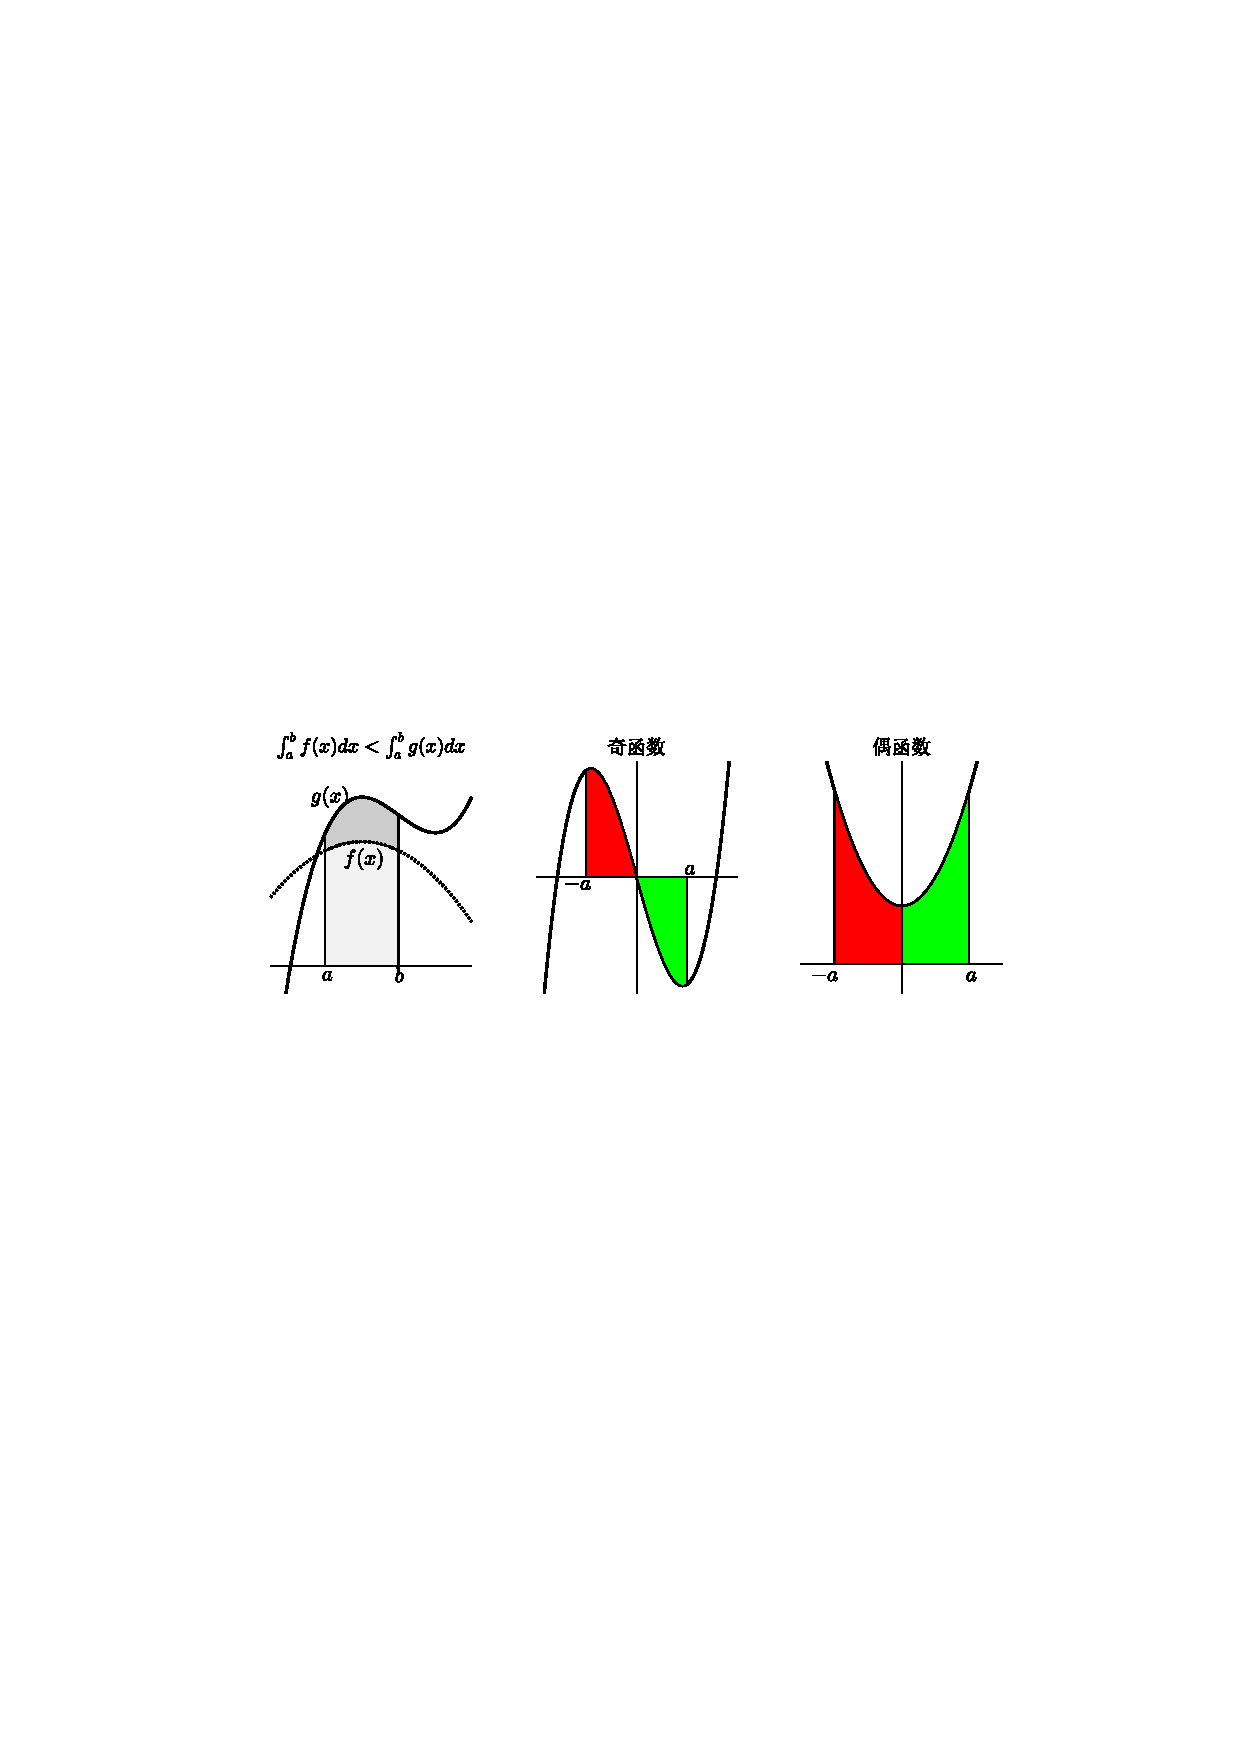
\includegraphics[width=0.9\linewidth]{定积分的一些性质}
\end{figure}  

% Hermite_Hadamard_BuDengShi.m
\item 厄米特-哈达玛(Hermite-Hadamard)不等式:
$ f(x) $在区间$ [a,b] $上连续且可积,\\ $ \forall x_1,x_2\in [a,b],\ 
x_1<x_2 $,如果$ f\Big(\dfrac{x_1+x_2}{2}\Big)<
\dfrac{1}{2}[f(x_1)+f(x_2)] $(等价于$ f''(x)>0 $),那么有 
\begin{gather}
    (x_2-x_1)\cdot f\left(\dfrac{x_1+x_2}{2}\right)<
    \int_{x_1}^{x_2}f(x)\d x<(x_2-x_1)\cdot \dfrac{f(x_1)+f(x_2)}{2} 
    \label{Hermite-Hadamard不等式0} \\
    f\left(\dfrac{x_1+x_2}{2}\right)<\dfrac{1}{x_2-x_1}
    \int_{x_1}^{x_2}f(x)\d x< \dfrac{f(x_1)+f(x_2)}{2}
    \label{Hermite-Hadamard不等式1}
\end{gather}
\begin{figure}[H]
    \centering
    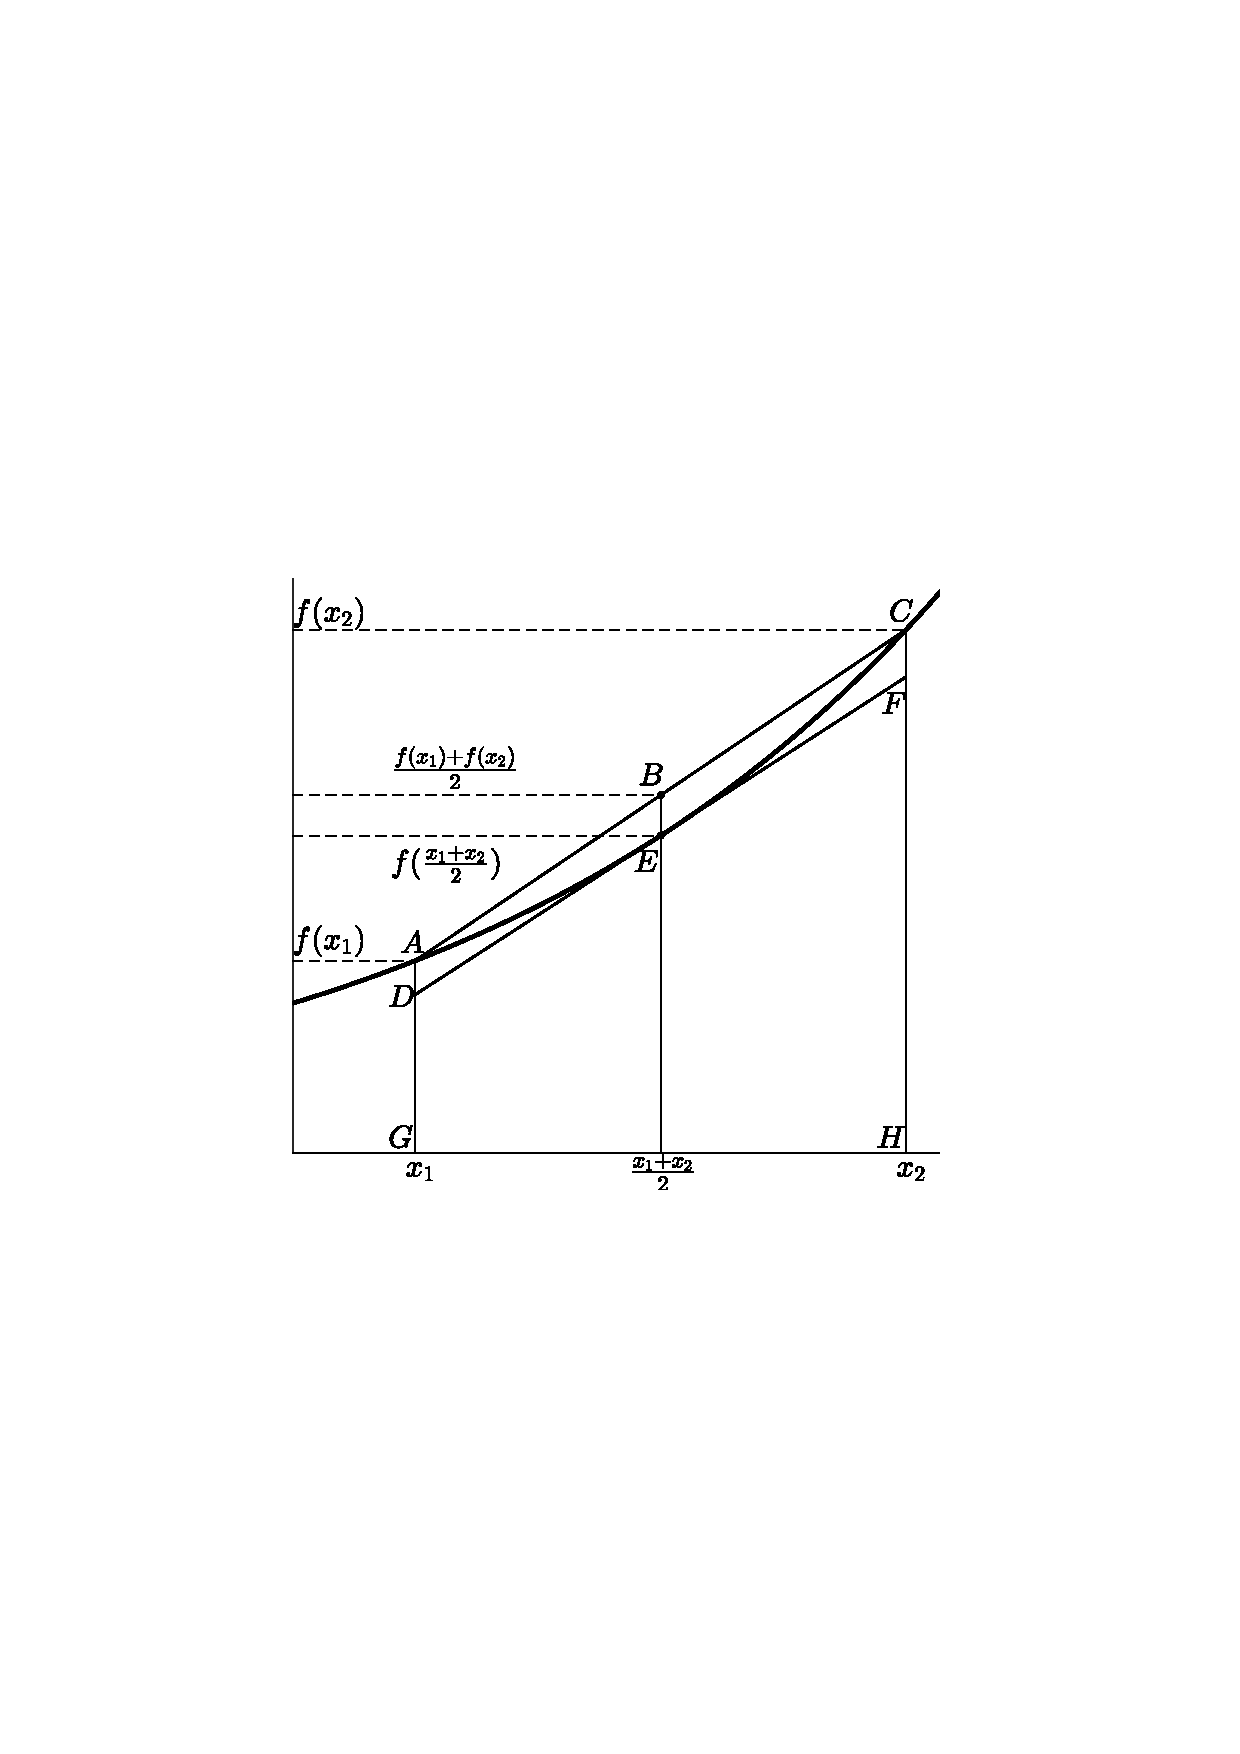
\includegraphics[width=0.5\linewidth]{Hermite-Hadamard不等式}
\end{figure}
$ E $点是直线$ x=\dfrac{x_1+x_2}{2} $与曲线$ y=f(x) $的交点,过$ E $点作
曲线$ y=f(x) $的切线,交$ AG $于$ D $点,交$ CH $于$ F $点。
在(\ref{Hermite-Hadamard不等式0})式中,

\hspace{0.6cm} $ (x_2-x_1)\cdot f\left(\dfrac{x_1+x_2}{2}\right) $
代表直角梯形$ ACHG $的面积,

\hspace{0.6cm} $ \disp \int_{x_1}^{x_2}f(x)\d x $代表曲边梯形$ AECHG $的面积,

\hspace{0.6cm} $ (x_2-x_1)\cdot \dfrac{f(x_1)+f(x_2)}{2} $
代表直角梯形$ DFHG $的面积,\\
结合上图,三个梯形的面积大小关系是显然的。

把(\ref{Hermite-Hadamard不等式1})式中的$ f(x) $换成$ f'(x) $,同时假定$ f'''(x)>0 $,那么有:
\begin{align}\label{Hermite-Hadamard不等式2}
    f'\left(\dfrac{x_1+x_2}{2}\right)<\dfrac{1}{x_2-x_1}
    \int_{x_1}^{x_2}f'(x)\d x=\dfrac{f(x_2)-f(x_1)}{x_2-x_1}< \dfrac{f'(x_1)+f'(x_2)}{2}
\end{align}
令$ f(x)=\ln x $,则$ f'''(x)=\dfrac{2}{x^3}>0 $,有
\begin{gather*}
    \dfrac{2}{x_1+x_2}<\dfrac{\ln x_2-\ln x_2}
    {x_2-x_1}<\dfrac{x_1+x_2}{2x_1x_2} \\
    \dfrac{2x_1x_2}{x_1+x_2}<\dfrac{x_2-x_1}{\ln x_2-
        \ln x_2}<\dfrac{x_1+x_2}{2}
\end{gather*}
令$ f(x)=\e^x $,则$ f'''(x)=\e^x>0 $,有
\begin{gather*}
    \e^{\frac{x_1+x_2}{2}}<\dfrac{\e^{x_2}-\e^{x_1}}{x_2-x_1}<
    \dfrac{\e^{x_1}+\e^{x_2}}{2}
\end{gather*} 

\item 下面这张表既是作为求导练习,也是作为积分表供查询。
\vspace{-3mm}
\begin{multicols}{2}
\noindent $ \ln\ln x \to \dfrac{1}{x\ln x} $ \\ 
$ \dfrac{1}{2}(\ln x)^2\to \dfrac{\ln x}{x} $ \\
$ \dfrac{1}{a}\ln(ax+b)\to \dfrac{1}{ax+b} $ \\ 
$ \dfrac{(ax+b)^{n+1}}{a(n+1)} \to (ax+b)^n $ \\ 
$ \dfrac{x}{a}-\dfrac{b}{a^2}\ln(ax+b) \to \dfrac{x}{ax+b}  $ \\ 
$ \dfrac{1}{b}\ln \left( \dfrac{x}{ax+b}\right) \to \dfrac{1}{x(ax+b)}   $ \\ 
$ \dfrac{1}{2a}\ln \left(\dfrac{x-a}{x+a} \right)\to\dfrac{1}{x^2-a^2} $ \\ 
$ \dfrac{1}{a}\arctan\dfrac{x}{a}\to\dfrac{1}{x^2+a^2} $ \\ 
$ \sqrt{a\pm x^2} \to \dfrac{\pm x}{\sqrt{a\pm x^2}} $ \\ 
$ \sqrt{a+b\cos x}\to \dfrac{-b\sin x}{2\sqrt{a+b\cos x}} $ \\ 
$ \ln(x+\sqrt{x^2+b}) \to \dfrac{1}{\sqrt{x^2+b}}   $ \\ 
$ \dfrac{x}{2}\sqrt{x^2+b}+\dfrac{b}{2}\ln(x+\sqrt{x^2+b})\to\sqrt{x^2+b} $\\ 
$ \dfrac{x^2}{2}\left(\ln x-\dfrac{1}{2} \right) \to x\ln x $ \\ 
$ \dfrac{x^{n+1}}{n+1}\left(\ln x-\dfrac{1}{n+1} \right) \to x^n\ln x $ \\ 
$ \arcsin \dfrac{x}{a} \to \dfrac{1}{\sqrt{a^2-x^2}}  $ \\ 
$ \dfrac{a^2}{2}\arcsin\dfrac{x}{a}+\dfrac{x}{2}\sqrt{a^2-x^2} \to \sqrt{a^2-x^2} $    
\end{multicols}

\item 用定义(用矩形法并求极限)计算$ \disp\int_{0}^{1}x^2\d x $.
\begin{align*}
    \int_{0}^{1}x^2\d x=&\lim_{n\to \infty}\left[\left(\dfrac{0}{n}\right)^2+
    \left(\dfrac{1}{n}\right)^2+\left(\dfrac{2}{n}\right)^2+
    \cdots+\left(\dfrac{n-1}{n}\right)^2\right]\dfrac{1}{n} 
    =\lim_{n\to \infty}\dfrac{1}{n^3}\sum_{k=1}^{n-1}k^2 \\
    =&\lim_{n\to \infty}\dfrac{1}{n^3}\left[ \dfrac{(n-1)^3}{3}+\dfrac{(n-1)^2}{2}
    +\dfrac{n-1}{6}\right] = \dfrac{1}{3}
\end{align*}

直接使用牛顿-莱布尼茨公式:$ \disp \int_{0}^{1}x^2\d x=\left.\dfrac{1}{3}x^3
\right|_0^1=\dfrac{1}{3} $. 

\item $ \disp \alpha>0,\ \int_{0}^{1}x^{\alpha}\d x=\left.\dfrac{1}{\alpha+1}
x^{\alpha+1}\right|_0^1=\dfrac{1}{\alpha+1} $. 

\item 用定义(用矩形法并求极限)计算$ \disp\int_{0}^{1}\e^x\d x $.
\begin{align*}
    \int_{0}^{1}\e^x\d x =&\ \lim_{n\to \infty}\left( \e^{\frac{0}{n}}+\e^{\frac{1}{n}}
    +\e^{\frac{2}{n}}+\cdots +\e^{\frac{n-1}{n}} \right)\dfrac{1}{n} 
    =\lim_{n\to \infty}\dfrac{1-\e}{1-\e^{\frac{1}{n}}}\cdot\dfrac{1}{n} \\ 
    =&\ (1-\e)\lim_{n\to \infty}\dfrac{\frac{1}{n}}{1-\e^{\frac{1}{n}}}  
    =(1-\e)\cdot (-1) =\e-1
\end{align*}
上面利用了重要的极限(\ref{(e^x-1)/x极限})式,即$ \lim\limits_{x\to 0}\dfrac{\e^x-1}{x}=1 $.

直接使用牛顿-莱布尼茨公式:$ \disp\int_{0}^{1}\e^x\d x=\left. \e^x\right|_0^1=\e-1 $. 

\item 用定义(用矩形法并求极限)计算$ \disp \int_{0}^{\pi}\sin x\d x $. 

\noindent\ \ 利用求和公式(\ref{正弦等差连加}),
\begin{align*}
    \int_{0}^{\pi}\sin x\d x =&\lim_{n\to \infty}\left[\sin\dfrac{\pi}{n}
    +\sin\dfrac{2\pi}{n}+\cdots +\sin \dfrac{(n-1)\pi}{n} \right]\dfrac{\pi}{n} \\
    =&\lim_{n\to \infty} \dfrac{-\cos(n+\dfrac{1}{2})\dfrac{\pi}{n}+\cos  \dfrac{\pi}{2n}}{2\sin \dfrac{\pi}{2n}}\cdot\dfrac{\pi}{n}  
    =\lim_{n\to \infty}\dfrac{\pi}{n\sin \dfrac{\pi}{2n}} 
    =\lim_{n\to \infty}\dfrac{\pi}{n\cdot \dfrac{\pi}{2n}} =2
\end{align*}
上面利用了重要的极限(\ref{sinx/x极限})式,即$ \lim\limits_{x\to 0}\dfrac{\sin x}{x}=1 $.

直接使用牛顿-莱布尼茨公式:$ \disp\int_{0}^{\pi}\sin x\d x=\left.-\cos x\right|_0^{\pi}
=2 $. 正弦函数一个拱下面的面积竟然是整数2,而没有包含无理数$ \pi $,还是比较神奇的。

\item $^*$ 正态分布(高斯分布)的概率密度函数为
$ f(x)=\dfrac{1}{\sqrt{2\pi}\sigma}\e^{-\frac{(x-\mu)^2}{2\sigma^2}} $,
已知$ \disp \int_{-\infty}^{\infty}\e^{-\frac{x^2}{a}}\d x=\sqrt{a\pi}\ (a>0) $,那么
\begin{align*}
    \int_{-\infty}^{\infty}f(x)\d x=\int_{-\infty}^{\infty}
    \dfrac{1}{\sqrt{2\pi}\sigma}\e^{-\frac{(x-\mu)^2}{2\sigma^2}}\d x=\dfrac{1}{\sqrt{2\pi}\sigma}
    \sqrt{2\sigma^2 \cdot \pi}=1
\end{align*}
概率密度函数$ f(x) $中之所以含有$ \dfrac{1}{\sqrt{2\pi}\sigma} $
这样一个系数,就是为了让上面的积分值为1(取遍所有情形的概率和为1). 

\item $ \dfrac{\sin x}{x},\ \dfrac{\cos x}{x},\ \dfrac{\e^x}{x},\ 
\dfrac{x}{\ln x},\ \dfrac{1}{\ln x},\ \sin(x^2),\ \cos(x^2),\ 
\e^{x^2},\ \sqrt{1-k^2\sin^2 x}\ (0<k<1) $均积不出原函数,或者说原函数不能用基本初等函数表示,但在某些特殊区间上的定积分精确值可能可以不通过原函数算出来
\footnote{要解释积不出来的原因,需要抽象代数中的域理论以及刘维尔(Liouville)定理,可查阅:\\
$ \diamond $ Liouville's theorem on integration in terms of elementary functions,\quad 
https://ksda.ccny.cuny.edu/PostedPapers/\\liouv06.pdf \\
$ \diamond $ Impossibility theorems for elementary integration,
\quad http://math.stanford.edu/\textasciitilde conrad/papers/elemint.pdf \\
$ \diamond $ 王建华,周丽萍. 某些不定积分的非初等性问题[J]. 
呼伦贝尔学院学报, 2005, 13(2):2.})。

\item 利用定积分对阶乘的增长速度做粗略估计:
\begin{align*}
    \ln n! &=\ln 1+\ln 2+ \cdots +\ln n 
    \approx \int_{3/2}^{n+1/2} \ln x\d x  
    =\left.(x\ln x - x)\right|_{3/2}^{n+1/2} \\
    &= \left[\left(n+\dfrac{1}{2}\right)
    \ln \left(n+\dfrac{1}{2}\right)-\left(n+\dfrac{1}{2}\right)\right]
    -\left[\dfrac{3}{2}\ln \dfrac{3}{2}-\dfrac{3}{2} \right] \\
    &=\left(n+\dfrac{1}{2}\right) \ln \left(n+\dfrac{1}{2}\right)
    -n+\underbrace{1-\dfrac{3}{2}\ln \dfrac{3}{2}}_{\approx 0.391802 }
\end{align*} 
\begin{align}
    n! &\approx \dfrac{\left(n+\dfrac{1}{2}\right)^
        {n+\frac{1}{2}}}{\e^n} \cdot \e^{0.391802}
    = \dfrac{n^{{n+\frac{1}{2}}} \left(1+\dfrac{1}{2n}\right)^
        {n+\frac{1}{2}}}{\e^n} \cdot \e^{0.391802} \nonumber\\ 
    &\approx \dfrac{n^{{n+\dfrac{1}{2}}} \left[1+\dfrac{1}{2n}
        \cdot\left(n+\dfrac{1}{2}\right)\right]}{\e^n}\cdot \e^{0.391802}
    \nonumber \\
    &\approx \dfrac{3}{2}\left(1+\dfrac{1}{6n}\right)\e^{0.391802}\sqrt{n}
    \left(\dfrac{n}{\e}\right)^n \\
    & \approx 2.219467\sqrt{n}\left(\dfrac{n}{\e}\right)^n
    \left(1+\dfrac{1}{6n}\right) \label{积分估计阶乘-系数2.219}
\end{align}

\item $^*$ 更精确的估计是下面的斯特林(Stirling)公式\footnote{《特殊函数概论》,
    第3.12节,渐进展开式。 }:
\begin{align}
    \ln n! &= \left(n+\dfrac{1}{2}\right)\ln n-n+\dfrac{1}{2}\ln(2\pi)+
    \sum_{r=1}^{N}\dfrac{(-1)^{r-1}B_{2r}}{2r(2r-1)n^{2r-1}}+O(n^{-2N-1}) \label{斯特林公式对数形式1-伯努利数} \\
    & \approx n(\ln n-1)+\dfrac{1}{2}\ln(2\pi n)+\dfrac{1}{12n}-
    \dfrac{1}{360n^3}+\dfrac{1}{1260n^5}-\dfrac{1}{1680n^7}+\cdots 
    \label{斯特林公式对数形式2}
\end{align}
其中$ B_{2r} $是伯努利数,上式取指数函数,得
\begin{gather}\label{斯特林公式指数形式}
    n!\approx \sqrt{2\pi n}\left(\dfrac{n}{\e}\right)^n \left(1+
    \dfrac{1}{12n}+\dfrac{1}{288n^2}-\dfrac{139}{51840n^3}-
    \dfrac{571}{2488320n^4}+\cdots \right)   
\end{gather}
$ \sqrt{2\pi}\approx 2.506628 $,稍大于(\ref{积分估计阶乘-系数2.219})
式中的$ 2.219467 $.当$ n $很大时,可近似取$ n!\approx \sqrt{2\pi n}\left(\dfrac{n}{\e}\right)^n $.

\item 关于$ n! $,还有如下不等式\footnote{Hsu L C ,  Luo X . On a 
    Two-sided Inequality Involving Stirling's Formula[J]. JOURNAL OF MATHEMATICAL RESEARCH AND EXPOSITION, 1999, 19(3):491-494.}:
\begin{gather}\label{阶乘-斯特林不等式}
    \sqrt{2\pi n}\left(\dfrac{n}{\e}\right)^n \left(1+\dfrac{1}{12n}\right)
    <n!<\sqrt{2\pi n}\left(\dfrac{n}{\e}\right)^n \left(1+
    \dfrac{1}{12n-0.5}\right)
\end{gather}

\item $^*$ $ \sqrt[n]{n!} $是一个严格单调递增的数列,
$ \dfrac{\sqrt[n]{n!}}{n+1} $是一个严格递减的数列。\\


\end{itemize}

\section{正整数的幂求和与黎曼zeta函数}
\begin{itemize}[leftmargin=\inteval{\myitemleftmargin}pt,itemsep=
   \inteval{\myitemitempsep}pt,topsep=\inteval{\myitemtopsep}pt]
\item $ \sum\limits_{l=1}^{n} l^k $的计算方法:用多个形如
$ (n+1)^{k+1}-n^{k+1} =(k+1)n^k+\dfrac{k(k+1)}{2}n^{k-1}+\cdots +1 $
的式子累加,再利用更低次数求和的已知结果。以$ k=2 $为例,
\begin{align*}
    (n+1)^3-n^3 =&3n^2+3n+1 \\
    n^3-(n-1)^3 =&3(n-1)^2+3(n-1)+1 \\
    &\cdots \\
    3^3-2^3 =&\ 3\cdot 2^2+3\cdot 2 +1 \\    
    2^3-1^3 =&\ 3\cdot 1^2+3\cdot 1 +1    
\end{align*}
将以上$ n $个式子相加:
\begin{align*}
    (n+1)^3-1=3\sum_{l=1}^{n} l^2+\dfrac{3n(n+1)}{2}+n
\end{align*}
移项整理后即可得$ \sum\limits_{l=1}^{n} l^2 $的结果。
\item 或者用待定系数法,仍以$ k=2 $为例,
假设$ \sum\limits_{l=1}^{n} l^2=an^3+bn^2+cn+d=f(n) $,
那么$ f(n) $必须满足$ f(n)-f(n-1)=n^2 $,即
\begin{align*}
    &\ a[n^3-(n-1)^3]+b[n^2-(n-1)^2]+c[n-(n-1)] \\
    =&\ 3an^2+(-3a+2b)n+(a-b+c) \\
    =&\ n^2
\end{align*}
于是$ 3a=1,\ -3a+2b=0,\ a-b+c=0 $,解得$ a=\dfrac{1}{3},\ b=\dfrac{1}{2},\ c=
\dfrac{1}{6} $.再由$ f(1)=a+b+c+d=1 $可得$ d=0 $. 

\item 下面给出$ 1\sim 6 $次方的求和结果:
\begin{align}
    1^1+2^1+3^1+\cdots +n^1 &=\dfrac{n^2}{2}+\dfrac{n}{2} =\dfrac{1}{2}n(n+1)
    \label{正整数1次方求和}\\
    1^2+2^2+3^2+\cdots +n^2&=\dfrac{n^3}{3}+\dfrac{n^2}{2}+\dfrac{n}{6}
    =\dfrac{1}{6}n(n+1)(2n+1)
    \label{正整数2次方求和} \\
    1^3+2^3+3^3+\cdots +n^3&=\dfrac{n^4}{4}+\dfrac{n^3}{2}+\dfrac{n^2}{4}=
    \left[\dfrac{1}{2}n(n+1) \right]^2 \label{正整数3次方求和}\\
    1^4+2^4+3^4+\cdots +n^4&=\dfrac{n^5}{5}+\dfrac{n^4}{2}+
    \dfrac{n^3}{3}-\dfrac{n}{30} 
            \label{正整数4次方求和} \\
    &=\dfrac{1}{30}n(n+1)(2n+1)(3n^2+3n-1) \notag\\
      1^5+2^5+3^5+\cdots +n^5&=\dfrac{n^6}{6}+\dfrac{n^5}{2}+
      \dfrac{5n^4}{12}-\dfrac{n^2}{12} \label{正整数5次方求和}\\
    &=\dfrac{1}{12}n^2(n+1)^2(2n^2+2n-1) \notag\\
    1^6+2^6+3^6+\cdots +n^6
    &=\dfrac{n^7}{7}+\dfrac{n^6}{2}+\dfrac{n^5}{2}-
    \dfrac{n^3}{6}+\dfrac{n}{42}
     \label{正整数6次方求和} \\
    &=\dfrac{1}{42}n(n+1)(2n+1)(3n^4+6n^3-3n+1)\notag 
\end{align}
规律\footnote{这个规律曾被作为2008年湖北高考理科数学的填空题。}:$ \sum\limits_{l=1}^{n} l^k \ (k\in \textbf{N}^+) $最高次项系数是
$ \dfrac{1}{k+1} $(因为$ \disp \int_0^n x^k\d x=\dfrac{n^{k+1}}{k+1} $,
这就是求和的主要部分),第二高次项系数是$ \dfrac{1}{2} $,第三高次项系数是$ \dfrac{k}{12} \cdots$这些求和公式可以写成如下通式,
\begin{align}\label{正整数k次方求和通式}
    1^k+2^k+3^k+\cdots +n^k=\dfrac{1}{k+1}
    \sum_{j=0}^{k}C_{k+1}^{j}B_{j}n^{k+1-j}+n^{k}
\end{align}
$ B_j $为伯努利数\footnote{伯努利数定义如下:$ \dfrac{x}{\e^x-1}=
    \sum\limits_{n=0}^{\infty}B_n\dfrac{x^n}{n!} $.可参看《特殊函数概论》第1页。},
$ B_0=1,B_1=-\dfrac{1}{2},B_2=\dfrac{1}{6},B_3=0,B_4=-\dfrac{1}{30},
B_5=0,B_6=\dfrac{1}{42}\cdots$
伯努利数满足递推关系:$ 0=\sum\limits_{j=0}^{n-1}C_n^jB_j\ (n\geq 2) $.\ 
(\ref{正整数k次方求和通式})式实际上是欧拉-麦克劳林公式\footnote{可参看《特殊函数概论》第6页。}的一个特例。
将(\ref{正整数k次方求和通式})式右侧的$ k+1 $次多项式定义为$ S(n,k+1) $,
那么当$ k\geq 2 $时,若$k$是偶数,
则$ S(n,k) $经过因式分解后总会包含$ \left[\dfrac{1}{2}n(n+1)\right]^2 $;
若$k$是奇数,则$ S(n,k) $经过因式分解后总会包含
$ \dfrac{1}{6}n(n+1)(2n+1) $.
将$ S(n,k) $对变量$ n $求偏导\footnote{此时可以假想$ n $是连续变量。},
也能发现一些规律,比如
\begin{align*}
    S(n,6) =&\ \dfrac{n^6}{6} +\dfrac{n^5}{2}+\dfrac{5n^4}{12}-\dfrac{n^2}{12}\\
    \dfrac{\partial S}{\partial n}(n,6)=&\ n^5+\dfrac{5n^4}{2}+
    \dfrac{5n^3}{3}-\dfrac{n}{6}=5S(n,5)+B_5 \\
    S(n,5) =&\ \dfrac{n^5}{5}+\dfrac{n^4}{2}+\dfrac{n^3}{3}-\dfrac{n}{30} \\
    \dfrac{\partial S}{\partial n}(n,5)=&\ n^4+2n^3+n^2-\dfrac{1}{30}=4S(n,4)+B_4
\end{align*}
该规律就是:$ \dfrac{\partial S}{\partial n}(n,k+1)=kS(n,k)+B_k $,证明如下:
\begin{align*}
    &\ \dfrac{\partial S}{\partial n}\left(\dfrac{1}{k+1}\sum_{j=0}^{k}
    C_{k+1}^{j}B_{j}n^{k+1-j}+n^{k}\right)-B_k\\
    =&\ \sum_{j=0}^{k}\dfrac{k+1-j}{k+1}C_{k+1}^{j}B_{j}n^{k-j}+kn^{k-1}-B_k \\
    =&\ \sum_{j=0}^{k-1}C_{k}^{j}B_{j}n^{k-j}+kn^{k-1} \\
    =&\ k\left(\dfrac{1}{k}\sum_{j=0}^{k-1}C_{k}^{j}B_{j}n^{k-j}+n^{k-1} \right)  \\
    =&\ kS(n,k)
\end{align*}
上面用到了$ \dfrac{k+1-j}{k+1}C_{k+1}^j=\dfrac{k+1-j}{k+1}\cdot
\dfrac{(k+1)!}{(k+1-j)!j!}=\dfrac{k!}{(k-j)!j!}=C_k^j $.
\item 用数学归纳法证明(\ref{正整数k次方求和通式})式,
固定$ k $,对$ n $进行归纳。\\
\mycircled{1}当$ n=1 $时,利用伯努利数满足递推关系:$ 0=\sum\limits_{j=0}^{k-1}C_k^jB_j\ (n\geq 2) $,有
\begin{align*}
    S(1,k)=\dfrac{1}{k}\sum_{j=0}^{k-1}C_{k}^{j}B_{j}+1=1
\end{align*}
\mycircled{2}假设在$ n $时结论成立,然后只需证明$ S(n,k)+(n+1)^{k-1}=S(n+1,k) $,即
\begin{align*}
    \dfrac{1}{k}\sum_{j=0}^{k-1}C_{k}^{j}B_{j}n^{k-j}+n^{k-1}+(n+1)^{k-1}
    =\dfrac{1}{k}\sum_{j=0}^{k-1}C_{k}^{j}B_{j}(n+1)^{k-j}+(n+1)^{k-1}
\end{align*}
下面来完成对$ kn^{k-1} =\sum\limits_{j=0}^{k-1}C_{k}^{j}B_{j}\left[
(n+1)^{k-j}-n^{k-j}\right] $的证明。
{\small \begin{align*}
        \sum\limits_{j=0}^{k-1}C_{k}^{j}B_{j}\left[(n+1)^{k-j}-n^{k-j}\right] 
        \hspace{5.8cm} &  \\
        = C_k^0B_0\left(C_k^1n^{k-1}+C_k^2n^{k-2}+C_k^3n^{k-3}+C_k^4n^{k-4}+\cdots+C_k^{k-1}n+C_k^k\quad \right) &\\
        + C_k^1B_1\left(C_{k-1}^1n^{k-2}+C_{k-1}^2n^{k-3}+C_{k-1}^3n^{k-4}+\cdots+C_{k-1}^{k-2}n
        + C_{k-1}^{k-1}\right) & \\
        + C_k^2B_2\left(C_{k-2}^1n^{k-3}+C_{k-2}^2n^{k-4}+\cdots+C_{k-2}^{k-3}n
        + C_{k-2}^{k-2}\right) & \\
        +\cdots\ \ & \\
        + C_k^{k-2}B_{k-2}\left(C_2^1n+C_2^2 \right) & \\
        +C_k^{k-1}B_{k-1}C_1^1 & \\
        \hline
        =kn^{k-1}+\left(C_k^0B_0C_k^2+C_k^1B_1C_{k-1}^1\right)n^{k-2}+ 
        \left(C_k^0B_0C_k^3+C_k^1B_1C_{k-1}^2+C_k^2B_2C_{k-2}^1\right)n^{k-3}& \\
        +\cdots +   \left(C_k^0B_0C_k^{k-1}+C_k^1B_1C_{k-1}^{k-2}+\cdots+C_k^{k-2}B_{k-2}C_2^1\right)n
        & \\
        +\left(C_k^0B_0C_k^{k}+C_k^1B_1C_{k-1}^{k-1}+\cdots+C_k^{k-2}B_{k-2}C_2^2+
        C_k^{k-1}B_{k-1}C_1^1 \right) & \\
        =kn^{k-1}
\end{align*}}
上面的过程应用了如下性质:当$ m\geq 2$时,$ n^{k-m} $的系数是
\begin{align*}
    \sum_{j=0}^{m-1}C_k^jB_jC_{k-j}^{m-j}=&\sum_{j=0}^{m-1}\dfrac{k!}{(k-j)!j!}
    \cdot\dfrac{(k-j)!}{(k-m)!(m-j)!}B_j  \\
    =&\sum_{j=0}^{m-1}\dfrac{k!}{m!(k-m)!}\cdot\dfrac{m!}{j!(m-j)!}B_j 
    =C_k^m\sum_{j=0}^{m-1}C_m^jB_j =0
\end{align*}
所以,在$ n+1 $时,(\ref{正整数k次方求和通式})式也成立。

\item 以$ \sum\limits_{l=1}^{n} l^2 $为例讨论其奇数项与偶数项的和,
\begin{align*}
    & \sum\limits_{l=1}^{n} (2l)^2=4\sum\limits_{l=1}^{n} l^2=\dfrac{4n^3}{3}+2n^2+\dfrac{2n}{3}  \\
    & \sum\limits_{l=1}^{n} (2l-1)^2=4\sum\limits_{l=1}^{n} l^2-4\sum\limits_{l=1}^{n} l+n=
    \dfrac{4n^3}{3}-\dfrac{n}{3}
\end{align*}

\item 对于$ \sum\limits_{l=1}^{n} l^k $,假如把指数由整数$ k $
改为大于$ -1 $的非整数$ \alpha $,则没有精确求和公式,但有近似公式,
只需要在(\ref{正整数k次方求和通式})式中保留正幂项即可,
其中的组合数$ C_{\alpha+1}^j $按照推广的组合数来理解,即
$ C_{\alpha+1}^j=\dfrac{1}{j!}(\alpha+1)\alpha (\alpha-1)
\cdots (\alpha-j+2) $. 

$ \sum\limits_{l=1}^{n} l^{\alpha}\ (\alpha>-1) $的主要部分仍然是
$ \dfrac{n^{\alpha+1}}{\alpha+1} $,
第二项是$ \dfrac{1}{2}n^{\alpha} $,第三项(如果$ \alpha>1 $)
是$ \dfrac{1}{\alpha+1}C_{\alpha+1}^2 B_2 n^{\alpha-1}=
\dfrac{\alpha}{12}n^{\alpha-1} $,第四项是0(因为伯努利数$ B_3=0 $),
第五项(如果$ \alpha>3 $)是$ \dfrac{1}{\alpha+1}C_{\alpha+1}^4B_4n^{\alpha-3}
=-\dfrac{\alpha (\alpha-1)(\alpha-2)}{720}n^{\alpha-3},\cdots $,
举例如下
\begin{align*}
    &\sum\limits_{l=1}^{n} l^{-1/2}\approx 2n^{1/2}\\  
    &\sum\limits_{l=1}^{n} l^{-1/3}\approx \dfrac{3}{2}n^{2/3} \\   
    &\sum\limits_{l=1}^{n} l^{1/3}\approx \dfrac{3}{4}n^{4/3}+\dfrac{1}{2}n^{1/3} \\
    &\sum\limits_{l=1}^{n} l^{1/2}\approx \dfrac{2}{3}n^{3/2}+\dfrac{1}{2}n^{1/2} \\
    &\sum\limits_{l=1}^{n} l^{3/2}\approx \dfrac{2}{5}n^{5/2}+\dfrac{1}{2}n^{3/2}
    +\dfrac{1}{8}n^{1/2} \\
    &\sum\limits_{l=1}^{n} l^{5/2}\approx \dfrac{2}{7}n^{7/2}+\dfrac{1}{2}n^{5/2}
    +\dfrac{5}{24}n^{3/2} \\
    &\sum\limits_{l=1}^{n} l^{7/2}\approx \dfrac{2}{9}n^{9/2}+\dfrac{1}{2}n^{7/2}
    +\dfrac{7}{24}n^{5/2}-\dfrac{7}{384}n^{1/2} 
\end{align*}
这些公式的精度非常高,$ \alpha>0 $时,大致可以精确到整数部分。在以上公式中取$ n=1 $,并用右侧减去左侧,
结果依次为$ 1,\dfrac{1}{2},\dfrac{1}{4},\ \dfrac{1}{6},\ \dfrac{1}{40},\ -\dfrac{1}{168},
\ -\dfrac{5}{1152} $(这些数字的绝对值在递减),如果把这些常数都减去,那么以上公式的精度将更高,即
% NoIntegerPowerSum.m
\begin{align}
    &\sum\limits_{l=1}^{n} l^{-1/2}\approx 2n^{1/2}
    -1 \label{负二分之一次方求和}\\  
    &\sum\limits_{l=1}^{n} l^{-1/3}\approx \dfrac{3}{2}n^{2/3}-\dfrac{1}{2} 
    \label{负三分之一次方求和} \\     
    &\sum\limits_{l=1}^{n} l^{1/3}\approx \dfrac{3}{4}n^{4/3}
    +\dfrac{1}{2}n^{1/3}-\dfrac{1}{4} \label{三分之一次方求和}\\
    &\sum\limits_{l=1}^{n} l^{1/2}\approx \dfrac{2}{3}n^{3/2}
    +\dfrac{1}{2}n^{1/2}-\dfrac{1}{6} \label{0.5次方求和}\\
    &\sum\limits_{l=1}^{n} l^{3/2}\approx \dfrac{2}{5}n^{5/2}+\dfrac{1}{2}n^{3/2}
    +\dfrac{1}{8}n^{1/2}-\dfrac{1}{40} \label{1.5次方求和}\\
    &\sum\limits_{l=1}^{n} l^{5/2}\approx \dfrac{2}{7}n^{7/2}+\dfrac{1}{2}n^{5/2}
    +\dfrac{5}{24}n^{3/2}+\dfrac{1}{168} \label{2.5次方求和}\\
    &\sum\limits_{l=1}^{n} l^{7/2}\approx \dfrac{2}{9}n^{9/2}+\dfrac{1}{2}n^{7/2}
    +\dfrac{7}{24}n^{5/2}-\dfrac{7}{384}n^{1/2}+\dfrac{5}{1152}\label{3.5次方求和}
\end{align}
%(\ref{三分之一次方求和})$ \sim $ (\ref{3.5次方求和})式都可以精确到小数点后第二位(百分位)。
%想要精确地分析误差,则要用到下面将要讲到的斯托尔茨定理。

\noindent 下面来解释为什么(\ref{负二分之一次方求和})$ \sim $ (\ref{3.5次方求和})式能成立。
$ \sum\limits_{l=1}^{n} l^{\alpha} $的主要部分是$ \dfrac{n^{\alpha+1}}
{\alpha+1}\ (\alpha>-1) $,可从定积分估计的求和上界与下界的平均值的角度来理解,
\begin{align*}
    \int_0^n x^{\alpha}\d x= \dfrac{n^{\alpha+1}}{\alpha+1} < \sum\limits_{l=1}^{n} l^{\alpha}
    < \int_0^{n+1}x^{\alpha} \d x= \dfrac{(n+1)^{\alpha+1}}{\alpha+1}  
\end{align*}
函数$ f(x)=\dfrac{x^{\alpha+1}}{\alpha+1} $
在$ x=n $处的切线为$ g(x)=n^{\alpha}(x-n)+\dfrac{n^{\alpha+1}}{\alpha+1} $,
可以用$ g(n+1)=n^{\alpha}+\dfrac{n^{\alpha+1}}{\alpha+1} $近似代替$ f(n+1) $,
因为$ f(n)<\sum\limits_{l=1}^{n} l^{\alpha}<f(n+1) $,所以,用$ f(n) $
和$ f(n+1) $的平均值来代替$ \sum\limits_{l=1}^{n} l^{\alpha} $,将具有更高的精度。
$ \sum\limits_{l=1}^{n} l^{\alpha} \approx \dfrac{f(n)+f(n+1)}{2}\approx \dfrac{g(n)+g(n+1)}{2}=
g\left(n+\dfrac{1}{2}\right) =\dfrac{n^{\alpha+1}}{\alpha+1}+ \dfrac{1}{2}n^{\alpha} $.  

也可以把积分的起点和终点移动$ \dfrac{1}{2} $,
\begin{gather*}
    \sum\limits_{l=1}^{n} l^{\alpha} \approx \int_{1/2}^{n+1/2} x^{\alpha}\d x 
    \approx \dfrac{\left(n+\dfrac{1}{2}\right)^{\alpha+1}}{\alpha+1} 
    \approx g\left(n+\dfrac{1}{2}\right)=
    \dfrac{n^{\alpha+1}}{\alpha+1}+ \dfrac{1}{2}n^{\alpha}
\end{gather*}

\item 还可以利用斯托尔茨定理进行分析,当指数为正整数时,使用普通的二项式定理;
当指数不是正整数时,使用牛顿广义二项式定理(\ref{牛顿广义二项式定理})。

令$ a_n=1^k+2^k+3^k+\cdots +n^k,\ b_n=n^{k+1} $,那么
\begin{align*}
    & \lim_{n\to \infty}\dfrac{1^k+2^k+3^k+\cdots +n^k}{n^{k+1}} =
    \lim_{n\to \infty}\dfrac{a_n}{b_n}=
    \lim_{n\to \infty}\dfrac{a_n-a_{n-1}}{b_n-b_{n-1}}= \\
    & \lim_{n\to \infty}\dfrac{n^k}{n^{k+1}-(n-1)^{k+1}}=
    \lim_{n\to \infty}\dfrac{n^k}{C_{k+1}^1 n^k -C_{k+1}^2 n^{k-1}+\cdots} = \dfrac{1}{k+1}     
\end{align*}

令$ c_n=1^k+2^k+3^k+\cdots +n^k-\dfrac{n^{k+1}}{k+1},\ d_n=n^{k} $,那么
\begin{align*}
    & \lim_{n\to \infty}\dfrac{1^k+2^k+3^k+\cdots +n^k-\dfrac{n^{k+1}}{k+1}}{n^{k}} =
    \lim_{n\to \infty}\dfrac{c_n}{d_n}=
    \lim_{n\to \infty}\dfrac{c_n-c_{n-1}}{d_n-d_{n-1}} \\
    =&\ \lim_{n\to \infty}\dfrac{n^k-\dfrac{1}{k+1}\left[n^{k+1}-(n-1)^{k+1} \right] }{n^{k}-(n-1)^{k}} 
    =\lim_{n\to \infty}\dfrac{n^k-\dfrac{1}{k+1}\left(C_{k+1}^1 n^k-C_{k+1}^2 n^{k-1}+
        \cdots \right) }{C_{k}^1 n^{k-1}-C_{k}^2 n^{k-2}+ \cdots} \\
    = &\lim_{n\to \infty}\dfrac{\dfrac{1}{k+1}C_{k+1}^2 n^{k-1}- \cdots}
    {C_{k}^1 n^{k-1} - \cdots} = \dfrac{1}{2}      
\end{align*}
感兴趣的读者可继续研究$ \lim\limits_{n\to \infty}\dfrac{1^k+2^k+3^k+\cdots +n^k-\dfrac{n^{k+1}}{k+1}-\dfrac{1}{2}n^k}{n^{k-1}} $.

\item 考虑$ \lim\limits_{n\to \infty}\left[S(n,\alpha+1)-\sum\limits_{l=1}^{n} l^{\alpha}\right] $的极限是否存在。
以$ f_n=\dfrac{2}{3}n^{3/2}+\dfrac{1}{2}n^{1/2}-\sum\limits_{l=1}^{n} 
l^{1/2} $为例,下面将证明数列$ \{f_n\} $单调递增且有界。
\begin{align*}
    f_n-f_{n-1}=&\ \dfrac{2}{3}\left[n^{3/2}-(n-1)^{3/2}\right]
    +\dfrac{1}{2}\left[n^{1/2}-(n-1)^{1/2}\right]-n^{1/2} \quad (n\geq 2)\\
    =&\ \dfrac{2}{3}(\sqrt{n}-\sqrt{n-1})(n+\sqrt{n(n-1)}+n-1)
    +\dfrac{1}{2}(\sqrt{n}-\sqrt{n-1})-\sqrt{n} \\
    =&\ (\sqrt{n}-\sqrt{n-1})\left[\dfrac{4}{3}n+\dfrac{2}{3}
    \sqrt{n(n-1)}-\dfrac{1}{6}\right]-\sqrt{n} \\
    =&\ \dfrac{\dfrac{4}{3}n+\dfrac{2}{3}
        \sqrt{n(n-1)}-\dfrac{1}{6}}{\sqrt{n}+\sqrt{n-1}}-\sqrt{n} \\
    =&\ \dfrac{\dfrac{4}{3}n+\dfrac{2}{3}\sqrt{n(n-1)}-\dfrac{1}{6}-
        \sqrt{n}(\sqrt{n}+\sqrt{n-1})}{\sqrt{n}+\sqrt{n-1}} \\
    =&\ \dfrac{n-\dfrac{1}{2}-\sqrt{n(n-1)}}{3(\sqrt{n}+\sqrt{n-1})}
    =\dfrac{\sqrt{n^2-n+\dfrac{1}{4}}-\sqrt{n^2-n}}{3(\sqrt{n}+\sqrt{n-1})}>0 \\
    =&\ \dfrac{1}{12(\sqrt{n}+\sqrt{n-1})\left(\sqrt{n^2-n+\dfrac{1}{4}}+
        \sqrt{n^2-n}\right)} \\
    <&\ \dfrac{1}{12(\sqrt{n-1}+\sqrt{n-1})\left(\sqrt{n^2-2n+1}+\sqrt{n^2-2n+1}
        \right)}=\dfrac{1}{48(n-1)^{3/2}}
\end{align*}
\begin{align*}
    f_n=&\ (f_{n}-f_{n-1})+(f_{n-1}-f_{n-2})+\cdots+(f_{2}-f_{1})+f_1 \\
    <&\ \dfrac{1}{48}\left[\dfrac{1}{(n-1)^{3/2}}+\dfrac{1}{(n-2)^{3/2}}
    +\cdots+\dfrac{1}{1}\right]+\dfrac{1}{6} <\dfrac{1}{48}\zeta\left(
    \dfrac{3}{2}\right)+\dfrac{1}{6}=0.221091\cdots
\end{align*}
所以$ \{f_n\} $单调递增且不超过$ 0.221091\cdots $.其中,$ \zeta(s) $
代表黎曼zeta函数,定义如下,
\begin{align*}
\zeta(s)=
\begin{cases}
    \sum\limits_{n=1}^{\infty} \dfrac{1}{n^s}
    =\prod_{p\text{取遍所有质数}}\dfrac{1}{1-\frac{1}{p^s}}  & (\Re s>1)  \\
    \dfrac{1}{1-2^{1-s}}\sum_{n=1}^{\infty}
    \dfrac{(-1)^{n+1}}{n^s}  & (0\leq \Re s\leq 1,\ s\neq 1)   \\
    2^s\pi^{s-1}\sin\left(\dfrac{\pi s}{2}\right)\Gamma(1-s)
    \zeta(1-s) & (\Re s<0) 
\end{cases} 
\end{align*}

其中$ \disp \Gamma(s)=\int_{0}^{\infty}\e^{-t}t^{s-1}\d t $,代表伽玛函数,
是阶乘的推广,$ \Gamma(s+1)=s\Gamma(s),\ \Gamma(n+1)=n!\ 
(n\in \textbf{N}),\  \Gamma(1)=1,\ \Gamma\left(\dfrac{1}{2}\right)=\sqrt{\pi} $. 
特别地,$ \zeta(0)=-\dfrac{1}{2} $. 设$ n\in \textbf{N}^+ $,那么
\begin{gather*}
    \zeta(2n)=\dfrac{2^{2n-1}\pi^{2n}|B_{2n}|}{(2n)!},\q \zeta(-n)=-\dfrac{B_{n+1}}{n+1},\q \zeta(-2n)=0,
\end{gather*}
其中$ B_n $为伯努利数。$ \zeta(2)=\dfrac{\pi^2}{6}=1.644934\cdots $是一个十分有用的结果
\footnote{$ \diamond $巴塞尔问题:著名公式背后的惊人几何学,
    https://www.bilibili.com/video/av20400157/ \\
    $ \diamond $ 巴塞尔问题(Basel problem)的多种解法,
    https://www.cnblogs.com/misaka01034/p/BaselProof.html \\
    可以用$ \dfrac{23}{14}\approx 1.642857<\dfrac{227}{138}
    \approx 1.644927<\dfrac{\pi^2}{6}\approx1.644934 <\dfrac{51}{31}\approx
    1.645161<\dfrac{33}{20}=1.65 $等分数作为$ \dfrac{\pi^2}{6} $的近似值,
    这些分数是靠“连分数逼近”的方法找到的。}。
自变量$ s $取正偶数$ 2n $时的结果,可参看《特殊函数概论》
第87页,或者Wolfram Mathworld的Riemann Zeta Function条目;
自变量$ s $取正奇数时,没有简单的表达式。

下面介绍
\begin{align}\label{zeta函数交错级数计算}
    \zeta(s)=\dfrac{1}{1-2^{1-s}}\sum\limits_{n=1}^{\infty}
    \dfrac{(-1)^{n+1}}{n^s}
\end{align}
是如何得到的,在
\begin{align}\label{zeta函数基础定义1}
    \zeta(s)=\sum\limits_{n=1}^{\infty} \dfrac{1}{n^s}
\end{align}
两边同乘$ 2^{1-s} $,有
\begin{align}\label{zeta函数两边乘2的1-s}
    2^{1-s}\zeta(s)=\sum\limits_{n=1}^{\infty} \dfrac{2}{(2n)^s},
\end{align}
\eqref{zeta函数基础定义1}$ - $\eqref{zeta函数两边乘2的1-s}式,
\begin{align*}
    (1-2^{1-s})\zeta(s)=&\ \left(\dfrac{1}{1^s}+\dfrac{1}{2^s}+
    \dfrac{1}{3^s}+\dfrac{1}{4^s}+\cdots\right)-
    \left(\dfrac{2}{2^s}+\dfrac{2}{4^s}+
    \dfrac{2}{6^s}+\dfrac{2}{8^s}+\cdots\right)\\
    =&\ \dfrac{1}{1^s}-\dfrac{1}{2^s}+\dfrac{1}{3^s}-\dfrac{1}{4^s}+\cdots
\end{align*}
两边除以$ 1-2^{1-s} $即得\eqref{zeta函数交错级数计算}式,\eqref{zeta函数交错级数计算}式实际上也适用于$ \Re s>1 $时的函数值的计算。若要手工计算zeta函数的函数值,在取的项数相同的时候,\eqref{zeta函数交错级数计算}式也比\eqref{zeta函数基础定义1}式要精确得多。比如$ \zeta(3)=1.202056\cdots $,
\begin{align*}
    &\dfrac{1}{1^3}+\dfrac{1}{2^3}+\dfrac{1}{3^3}+\dfrac{1}{4^3} =1.177662\cdots \\
    \dfrac{1}{1-2^{1-3}}\Big( &\dfrac{1}{1^3}-\dfrac{1}{2^3}+\dfrac{1}{3^3}-
    \dfrac{1}{4^3}\Big) =1.195216\cdots
\end{align*}    
\\
%\item zeta函数的近似计算,将$ \zeta(s) $在$ s=1 $处展开成洛朗级数
%\footnote{参见 https://zhuanlan.zhihu.com/p/136328750 },
%\begin{align}
%    \zeta(s) &=\dfrac{1}{s-1}+\sum_{n=0}^{\infty}
%    \dfrac{(-1)^n\gamma_n}{n!}(s-1)^n \nonumber \\
%    &\approx \dfrac{1}{s-1}+\gamma_0-\gamma_1(s-1)
%    +\dfrac{1}{2}\gamma_2(s-1)^2 \nonumber \\
%    &\approx \dfrac{1}{s-1}+0.577215+ 0.072815(s-1)
%    -0.004845(s-1)^2  \nonumber \\
%    & \approx \dfrac{1}{s-1}+0.499555+0.082505s-0.004845s^2 
%    \label{zeta函数洛朗展开近似1} 
%\end{align}
%其中,
%\begin{gather*}
%    \gamma_n=\lim _{M \to \infty}\left[\sum_{k=1}^{M} 
%    \frac{(\ln k)^n}{k}-\frac{(\ln M)^{n+1}}{n+1}\right]
%\end{gather*}
%被称为斯蒂尔吉斯常数(Stieltjes constant).
%
%为了让读者在没有软件而只有计算器的情况下能使用更简单的近似公式,现在对
%(\ref{zeta函数洛朗展开近似1})式的系数作一些调整,把$ 0.499555 $近似成
%$ 0.5 $,把$ -0.004845 $近似成$ -0.005 $,然后借助软件找出比较合适的
%一次项系数,如下:
%\begin{align}
%    \zeta(s) \approx \dfrac{1}{s-1}+0.5+0.0824s-0.005s^2 
%    \label{zeta函数洛朗展开近似2}
%\end{align}
%
%下表是$ \zeta(s) $精确值,利用(\ref{zeta函数洛朗展开近似2})
%式计算的近似值,分别取前10项、20项、40项求和的对比,
%\begin{table}[H]
%    \centering
%    \begin{tabular}{|c|c|c|c|c|c|}
%        \hline
%        $ s $ & $ \zeta(s) $精确值 & (\ref{zeta函数洛朗展开近似2})
%        式近似值 & $ \sum\limits_{n=1}^{10}
%        \dfrac{1}{n^s} $ & $ \sum\limits_{n=1}^{20}\dfrac{1}{n^s} $ & 
%        $ \sum\limits_{n=1}^{40}\dfrac{1}{n^s} $ \\ \hline
%        1.5 & 2.612375 & 2.612350 & 1.995336 & 2.170682 & 2.298112 \\ \hline
%        2 & 1.644934 & 1.644800 & 1.549768 & 1.596163 & 1.620244 \\ \hline
%        2.5 & 1.341487 & 1.341417 & 1.321921 & 1.334307 & 1.338901 \\ \hline
%        3 & 1.202057 & 1.202200 & 1.197532 & 1.200868 & 1.201752 \\ \hline
%        3.5 & 1.126734 & 1.127150 & 1.125618 & 1.126524 & 1.126696 \\ \hline
%        4 & 1.082323 & 1.082933 & 1.082037 & 1.082285 & 1.082318 \\ \hline
%    \end{tabular}
%\end{table}
%\bigskip 
\noindent 一些zeta函数精确值计算如下:
\begin{align*}
    \zeta(3)=&\ \sum_{n=1}^{\infty} \dfrac{1}{n^3}=\dfrac{1}{2}\int_0^1 \dfrac{(\ln x)^2}{1-x}\d x=1.20205690315959\cdots \\
    \zeta(4)=&\ \sum_{n=1}^{\infty} \dfrac{1}{n^4}=\dfrac{\pi^4}{90}
    =1.08232323371114\cdots     \\ 
    \zeta\left(\dfrac{4}{3}\right)=&\ \sum_{n=1}^{\infty} \dfrac{1}{n^{4/3}}=
    3.600937750458862 \cdots\\
    \zeta\left(\dfrac{3}{2}\right)=&\ \sum_{n=1}^{\infty} \dfrac{1}{n^{3/2}}=
    2.612375348685488 \cdots\\
    \zeta\left(\dfrac{1}{3}\right)=&\ \dfrac{1}{1-2^{2/3}}\sum_{n=1}^{\infty}
    \dfrac{(-1)^{n+1}}{n^{1/3}}=-0.973360248350782\cdots \\
    \zeta\left(\dfrac{1}{2}\right)=&\ \dfrac{1}{1-2^{1/2}}\sum_{n=1}^{\infty}
    \dfrac{(-1)^{n+1}}{n^{1/2}}=-1.460354508809586\cdots \\
    \zeta\left(-\dfrac{1}{3}\right)=&\ 2^{-1/3}\pi^{-4/3}\sin\left(-\dfrac{\pi}{6}\right)
    \Gamma\left(\dfrac{4}{3}\right)\zeta\left(\dfrac{4}{3}\right)
    =-0.277343047840130\cdots  \\
    \zeta\left(-\dfrac{1}{2}\right)=&\ 2^{-1/2}\pi^{-3/2}\sin\left(-\dfrac{\pi}{4}\right)
    \Gamma\left(\dfrac{3}{2}\right)\zeta\left(\dfrac{3}{2}\right)
    = -0.207886224977355\cdots  \\
    \zeta\left(-1\right)=&\ 2^{-1}\pi^{-2}\sin\left(-\dfrac{\pi}{2}
    \right)\Gamma\left(2\right)\zeta\left(2\right)=-\dfrac{1}{12} \\
    \zeta\left(-3\right)=&\ 2^{-3}\pi^{-4}\sin\left(-\dfrac{3\pi}{2}
    \right)\Gamma\left(4\right)\zeta\left(4\right)=\dfrac{1}{120}    
\end{align*}
\text{注:} $ \Gamma\left(\dfrac{4}{3}\right)= 0.892979511569249\cdots $,
$ \Gamma\left(\dfrac{3}{2}\right)=\dfrac{1}{2}\Gamma\left(\dfrac{1}{2}\right)
=\dfrac{1}{2}\sqrt{\pi}=0.886226925452758\cdots $.

负偶数被称为zeta函数的平凡零点(因为$ \sin\left(\dfrac{\pi\cdot 
  (-2n)}{2}\right)=0 $),zeta函数的自变量还可以取复数,大名鼎鼎的黎曼猜想
\footnote{ 卢昌海所著的《黎曼猜想漫谈》一书,十分精彩而有趣,是我最喜欢的一本书,
    我愿称之为关于黎曼猜想的最好的科普读物,没有“之一”,
    强烈推荐对黎曼猜想感兴趣的读者去阅读。黎曼猜想是当今数学界最重要的猜想之一,
    证明这一猜想的困难程度无疑是巨大的。若干年后成功证明黎曼猜想的人,
    将会成为与牛顿、高斯、爱因斯坦齐名的人物,会被载入史册,永垂不朽,
    会收获人类世界的最高荣誉,但同时也会被无数的民科纠缠和攻击。}的内容是:
黎曼zeta函数的所有\textbf{非平凡零点}的\textbf{实部}都是$ \dfrac{1}{2} $. 

\item 类似于$ 0<f_n-f_{n-1}<\dfrac{1}{48(n-1)^{3/2}} $,可以证明:(以下$ n\geq 2 $)
\begin{align}
    &\ 2\left[n^{1/2}-(n-1)^{1/2}\right]-n^{-1/2}\nonumber\\ =&\
    \dfrac{1}{n^{1/2}\left[n^{1/2}+(n-1)^{1/2}\right]^2}
    <\dfrac{1}{4(n-1)^{3/2}} \label{负二分之一误差分析} \\
    &\ \dfrac{3}{2}\left[n^{2/3}-(n-1)^{2/3}\right]-n^{-1/3}\nonumber\\ =&\
    \dfrac{n^{1/3}+2(n-1)^{1/3}}{2n^{1/3}\left[n^{2/3}+n^{1/3}(n-1)^{1/3}+(n-1)
        ^{2/3}\right]^2} < \dfrac{1}{6(n-1)^{4/3}} \label{负三分之一误差分析}\\
    &\ \dfrac{3}{4}\left[n^{4/3}-(n-1)^{4/3}\right]+\dfrac{1}{2}\left[n^{1/3}
    -(n-1)^{1/3}\right]-n^{1/3} \nonumber \\ =&\ \dfrac{n^{1/3}+(n-1)^{1/3}}{4
        \left[n^{2/3}+n^{1/3}(n-1)^{1/3}+(n-1)^{2/3}\right]^3}<
    \dfrac{1}{54(n-1)^{5/3}}   \label{三分之一误差分析} \\
    &\ \dfrac{2}{3}\left[n^{3/2}-(n-1)^{3/2}\right]
    +\dfrac{1}{2}\left[n^{1/2}-(n-1)^{1/2}\right]-n^{1/2} \nonumber\\ =&\ 
    \dfrac{1}{12\left[n^{1/2}+(n-1)^{1/2}\right]\left[n-\dfrac{1}{2}+
        n^{1/2}(n-1)^{1/2}\right]}<\dfrac{1}{48(n-1)^{3/2}} \label{二分之一误差分析}
\end{align} \\
(\ref{负二分之一误差分析})、(\ref{负三分之一误差分析})、(\ref{三分之一误差分析})式中的
等式和不等式的证明留做习题。(\ref{三分之一误差分析})式中的不等式的证明难度较大,
可借助软件验证。

\item 事实上有下面的一般性结果\footnote{Maple软件也能给出这个符号结果,
而不仅是数值结果。研究这个问题要用到欧拉-麦克劳林公式,可参看
《特殊函数概论》第3.22节“$ \zeta $函数的计算”。 还可以参考以下文献:\\
$ \diamond $ 甘超一. 自然数分数幂数列近似求和初探[J].中学数学,1999:31-33.\\
$ \diamond $ 匡继昌. 有限和的渐近估计[J]. 河西学院学报, 2002, 18(2):8. \\
读者如果有高质量的、更容易读懂的文献,欢迎向我提供。}:
\begin{gather}\label{Maple发现的极限}
    \lim\limits_{n\to \infty} \left[ S(n,\alpha+1)
    -\sum\limits_{l=1}^{n} l^{\alpha}\right]=-\zeta(-\alpha)
\end{gather}
比如
\begin{align*}
    & \lim\limits_{n\to \infty}\left(2n^{1/2}
    -\sum\limits_{l=1}^{n} l^{-1/2}\right)=-\zeta\left(
    \dfrac{1}{2}\right) \approx 1.460354<\dfrac{1}{4}\zeta\left(
    \dfrac{3}{2}\right)+1=1.653093\cdots \\
    & \lim\limits_{n\to \infty}\left(\dfrac{3}{2}n^{2/3}
    -\sum\limits_{l=1}^{n} l^{-1/3}\right)=-\zeta\left(
    \dfrac{1}{3}\right) \approx 0.973360<\dfrac{1}{6}\zeta\left(
    \dfrac{4}{3}\right)+\dfrac{1}{2}=1.100156\cdots \\
    & \lim\limits_{n\to \infty}\left(\dfrac{3}{4}n^{4/3}+\dfrac{1}{2}
    n^{1/3}-\sum\limits_{l=1}^{n} l^{1/3}\right)=-\zeta\left(
    -\dfrac{1}{3}\right) \approx 0.277343<\dfrac{1}{54}\zeta\left(
    \dfrac{5}{3}\right)+\dfrac{1}{4}=0.289324\cdots \\    
    & \lim\limits_{n\to \infty} \left(\dfrac{2}{3}n^{3/2}+
    \dfrac{1}{2}n^{1/2}-\sum\limits_{l=1}^{n} l^{1/2}\right)
    =-\zeta\left(-\dfrac{1}{2}\right)\approx 0.207886
    <\dfrac{1}{48}\zeta\left(
    \dfrac{3}{2}\right)+\dfrac{1}{6}=0.221091\cdots
\end{align*}
于是有以下两边夹的不等式,这些不等式也说明了为什么(\ref{负二分之一次方求和})$ \sim $
(\ref{3.5次方求和})式大致可以精确到整数部分。
\begin{align}
    2n^{1/2}\underbrace{-\dfrac{19}{13}}_{\approx -1.4615}
    <2n^{1/2}+\underbrace{\zeta\left(\dfrac{1}{2}\right)}_{\approx -1.4604}
    < &\ \sum\limits_{l=1}^{n} l^{-1/2}\leq 2n^{1/2}-1  \\  
    \dfrac{3}{2}n^{2/3}\underbrace{-\dfrac{37}{38}}_{\approx -0.9737}
    <\dfrac{3}{2}n^{2/3}+
    \underbrace{\zeta\left(\dfrac{1}{3}\right)}_{\approx -0.9734}
    < &\ \sum\limits_{l=1}^{n} l^{-1/3}\leq \dfrac{3}{2}n^{2/3}-\dfrac{1}{2}  \\ 
    \dfrac{3}{4}n^{4/3}+\dfrac{1}{2}n^{1/3}
    \underbrace{-\dfrac{5}{18}}_{\approx -0.2778}
    <\dfrac{3}{4}n^{4/3}+\dfrac{1}{2}n^{1/3}+
    \underbrace{\zeta\left(-\dfrac{1}{3}\right)}_{\approx -0.2773}   
    < &\ \sum\limits_{l=1}^{n} l^{1/3}\leq \dfrac{3}{4}n^{4/3}
    +\dfrac{1}{2}n^{1/3}-\dfrac{1}{4}  \\
    \dfrac{2}{3}n^{3/2}+\dfrac{1}{2}n^{1/2}
    \underbrace{-\dfrac{5}{24}}_{\approx -0.2083}
    <\dfrac{2}{3}n^{3/2}+\dfrac{1}{2}n^{1/2}+
    \underbrace{\zeta\left(-\dfrac{1}{2}\right)}_{\approx -0.2079}  
    < &\ \sum\limits_{l=1}^{n} l^{1/2}\leq \dfrac{2}{3}n^{3/2}
    +\dfrac{1}{2}n^{1/2}-\dfrac{1}{6} 
\end{align}

\item (\ref{负二分之一误差分析})$ \sim $(\ref{二分之一误差分析})式中的$ < $也可看成是
$ \approx $,借此可以进一步提高(\ref{负二分之一次方求和})$ \sim $(\ref{3.5次方求和})
式的精度,以(\ref{负二分之一误差分析})式为例进行分析,
\begin{align*}
    2n^{1/2}-\sum_{l=1}^{n}l^{-1/2}\approx 1+\sum_{l=2}^{n}\dfrac{1}{4(l-1)^{3/2}} 
    =&\ 1+\dfrac{1}{4}\zeta\left(\dfrac{3}{2}\right)-\dfrac{1}{4}\sum_{l=n+1}^{\infty}
    \dfrac{1}{(l-1)^{3/2}} \\
    \approx&\ 1+\dfrac{1}{4}\zeta\left(\dfrac{3}{2}\right)-
    \dfrac{1}{4}\int_n^{\infty}\dfrac{\d x}{x^{3/2}} \\
    =&\ 1+\dfrac{1}{4}\zeta\left(\dfrac{3}{2}\right)-\dfrac{1}{2}n^{-1/2}
\end{align*}
再把常数$ 1+\dfrac{1}{4}\zeta\left(\dfrac{3}{2}\right) $替换成真正的极限
$ -\zeta\left(\dfrac{1}{2}\right) $,可得,
\begin{gather} \label{负二分之一次方求和-带负幂项}
    \sum_{l=1}^{n}l^{-1/2}\approx 2n^{1/2}+\dfrac{1}{2}n^{-1/2}+
    \zeta\left(\dfrac{1}{2}\right)
\end{gather}
类似地有,
\begin{align}
    &\sum\limits_{l=1}^{n} l^{-1/3}\approx \dfrac{3}{2}n^{2/3}+\dfrac{1}{2}n^{-1/3}
    +\zeta\left(\dfrac{1}{3}\right)  \label{负三分之一次方求和-带负幂项} \\     
    &\sum\limits_{l=1}^{n} l^{1/3}\approx \dfrac{3}{4}n^{4/3}
    +\dfrac{1}{2}n^{1/3}+\dfrac{1}{36}n^{-2/3}
    +\zeta\left(-\dfrac{1}{3}\right)  \label{三分之一次方求和-带负幂项} \\
    &\sum\limits_{l=1}^{n} l^{1/2}\approx \dfrac{2}{3}n^{3/2}
    +\dfrac{1}{2}n^{1/2}+\dfrac{1}{24}n^{-1/2}
    +\zeta\left(-\dfrac{1}{2}\right)  \label{0.5次方求和-带负幂项}
\end{align}
可以发现,负幂项的系数还是延续了指数为正整数时的规律,即
\begin{gather*}
    \dfrac{1}{\alpha+1},\q   \dfrac{1}{2},\q  \dfrac{\alpha}{12},\q 
    0,\q  -\dfrac{\alpha (\alpha-1)(\alpha-2)}{720}\cdots
\end{gather*}
比如$ \dfrac{1}{36}=\dfrac{1}{12}\times\dfrac{1}{3},\  \dfrac{1}{24}=
\dfrac{1}{12}\times\dfrac{1}{2} $. 

\item 考虑$ \sum\limits_{l=1}^{n} (l+\delta)^k $和$ \sum\limits_{l=1}^{n}
(l+\delta)^{\alpha} $,前一种情况比较简单,直接使用二项式定理即可;后一种情况,
则直接在$ \sum\limits_{l=1}^{n} l^{\alpha} $的近似求和公式(\ref{负二分之一次方求和})
$ \sim $(\ref{3.5次方求和})中把$ n $换成$ n+\delta $即可\footnote{
 这个问题可借助Maple做研究,$ n\to \infty $
 时的极限同样存在,且可以用推广的zeta函数$ \zeta(s,a) =\sum\limits_{n=0}^{\infty}\dfrac{1}{(n+a)^s} $表示。},比如
\begin{gather*}
    \sum\limits_{l=1}^{n} (l+0.5)^{1/2}\approx \dfrac{2}{3}(n+0.5)^{3/2}
    +\dfrac{1}{2}(n+0.5)^{1/2}-\dfrac{1}{2}\cdot 1.5^{1/2}
\end{gather*}

%\newpage 
\end{itemize}

\section{例题}
\noindent \textbf{面对导数的大题}
\begin{itemize}[itemsep=-1pt]
\item 确定函数的定义域,观察函数的零点。
\item 有时候是直接对题目中的函数求导,有时候需要先分离参数再求导。
\item 观察导函数能否进行因式分解,如果可以,那就进行因式分解,这样使得符导数的正负号判断更加容易。
\item 如果原函数或导函数的零点解不出来,那就首先考虑估计零点的范围,这个范围越小越好。后续的计算过程中几乎总是要做一些关于零点的代换,使得需要求导的函数更加简单。
\item 如果一阶导数的单调性和正负号不容易确定,那就求二阶导数。如果一阶导数是分式型函数,且分母的正负号是确定的,那就把分子单独拿出来求导,而不要对这个分式型函数继续求导。
\item 如果要使用课本上未出现过的不等式,则需要先作出(简要的)证明。但是,
凡是规定高考中不允许出现二阶以及更高阶导数符号的人,都是教育界的悲哀和耻辱!
\item 要证明$ f(x)>g(x) $,首选方案是构造函数$ F(x)=f(x)-g(x) $,
然后令$ F'(x)=0 $找出极小值点,只要$ [F(x)]_{\min}>0 $,就完成了证明。
如果$ f(x),g(x) $都是不变号的(比如在给定区间上恒为正),且两者中恰好有一个是
$ \e^x $,比如要证$ f(x)>\e^x $,
还可以构造函数$ G(x)=f(x)\e^{-x} $,然后证明$ [G(x)]_{\min}>1 $. 
$ G'(x)=[f'(x)-f(x)]\e^{-x} $,当$ f(x) $为多项式时,$ f'(x)-f(x) $的零点容易求出。
\item 对于难度较大的题目,如果能想出高中阶段的解法,那肯定是首选。想不出高中方法,但能用大学的方法或定理解决的,也还是写到答题卡上,总比留空白要强
\footnote{关于在高考的大题中使用大学的方法和定理是否会被扣分,并不能给出一个十分肯定的回答,需要视情况而定。如果直接使用大学的定理,而没有任何推导和计算过程,几乎可以肯定得0分(尤其是证明题,以配极原理、彭赛列闭合定理为代表)。如果使用了大学的定理,但也包含了足够的、正确的计算过程,则可能少量扣分,也可能拿满分(以罗必塔法则、泰勒级数、帕德逼近、拉格朗日中值定理、平面的截距式方程、琴森不等式为代表)。如果你想在立体几何的大题中用二重积分计算体积、用曲面积分计算面积来炫技,笔者建议先用高中方法写一遍解答,再把积分作为第二种解法来炫技。}。
\item 对于以后想从事真正的数学研究的人而言,凡是有通用的解决方法,只是手算很困难,但借助计算机软件可以轻易解决的问题,都是毫无研究价值的,不值得花过多时间。那些靠计算机也无法解决,或者需要很长的计算时间才能解决的问题,才可能具有研究价值。比如某个函数求导后的零点靠手算很难算出来,正负号难以判断,钻研此类问题对考试有一定的帮助,对更高等级的数学学习毫无帮助。
\end{itemize}

\bigskip

\noindent 在本章的例题和习题中,$ \e $一律指代自然对数的底数
$ 2.718281828\cdots $,没有其它含义。

\begin{enumerate}[label={【\textbf{例\thechapter.\arabic*}】},
 leftmargin=\inteval{\myenumleftmargin}pt,
 itemsep=\inteval{\myenumitempsep}pt,
 itemindent=\inteval{\myenumitemindent}pt]
\item 当$ x\geq 2 $时,比较$ \log_x (x+1) $与
$ \log_{x+1} (x+2) $的大小。\\
\textbf{解}\ 令$ f(x)=\log_x (x+1)=\dfrac{\ln (x+1)}{\ln x}=\dfrac{\ln x
	+\ln\left(1+\dfrac{1}{x}	\right)}{\ln x}=1+\dfrac{\ln\left(1+\dfrac{1}{x}
	\right)}{\ln x} $,显然,$ f(x) $在$ [2,+\infty) $上递减,所以 $ \log_x (x+1)>\log_{x+1} (x+2) $. 

或者求导,$ f'(x)=\dfrac{\dfrac{\ln x}{x+1}-\dfrac{\ln(x+1)}{x}}
{\ln^2 x}  <0 $.导数的分子小于0是显然的。 

\item\label{比大小问题999_998} 比较$ 999^{998} $与$ 998^{999} $的大小。\\
\textbf{解}\ $ \left( \dfrac{\ln x}{x} \right)'=\dfrac{1-\ln x}{x^2}  $,所以$ 
\dfrac{\ln x}{x} $在$ [\e,+\infty) $上递减,故$ \dfrac{\ln 999}{999} < \dfrac{\ln 998}{998}$, $ 998\ln999 < 999\ln 998 $, $ 999^{998} < 998^{999} $. 

$ \dfrac{\ln x}{x} $可看成是对数函数$ y=\ln x $图像上的某一点
与原点连线的斜率,斜率的最大值在相切(切线为$ y=\dfrac{x}{\e} $)的时候取得。

对于允许在高考中使用计算器的省份,一般的计算器也无法计算$ 998^{999} $,需要做一些变换,
比如算出$ 998\ln999 \approx 6892.94 < 999\ln 998 \approx 6898.85  $,
或者算出$ 999^{998/999}\approx 992.11 < 998 $,
或者算出$ \left(\dfrac{999}{998} \right)^{998}\cdot \dfrac{1}{998}\approx \dfrac{2.716921}{998}<1 $.

\item 分别用割线法、切线法、迭代法估算$ \sqrt{73} $
(精确值$ 8.544003745317530 \cdots $)
\footnote{73是第21个素数,把73倒序得到37,37是第12个素数,12恰好是21的倒序,
这可以称为“镜像性”。同时,$ 7\times 3=21 $,这可以称为“积性”。
73的这两个性质最初是美剧《生活大爆炸》中的谢尔顿(Sheldon)提出的(严格来讲,
应该是编剧提出来的),后来,同时具备镜像性和积性的素数被称为谢尔顿素数
(Sheldon prime),Jessie Byrnes在下列2015年的论文中提出了猜想:
73是唯一的谢尔顿素数。Carl Pomerance在下列2019年的论文中证明了这一猜想。\\
$ \diamond $ Jessie Byrnes, Chris Spicer, Alyssa Turnquist. The Sheldon conjecture. Math Horizons. 2015,23(2):12–15.
doi.org/10.4169/mathhorizons.23.2.12 \\
$ \diamond $ Carl Pomerance, Chris Spicer, Proof of the Sheldon Conjecture, The American Mathematical Monthly[J]. 2019,
126(8):688-698. doi.org/10.1080/00029890.2019.1626672 } \\
\textbf{解}\ $ 64<73<81 $ .\\
割线近似值(偏小):$ 8+\dfrac{73-64}{2\times 8+1}=8+\dfrac{9}{17}\approx 8.529412 $ \\
切线近似值(偏大):$ 8+\dfrac{73-64}{2\times 8}=8+\dfrac{9}{16}= 8.562500 $ \\
更好近似值:$ 8+\dfrac{73-64}{2\times 8+0.5}=8+\dfrac{9}{16.5}\approx 8.545454 $ \\
迭代近似值:$ a_1=8,a_2=8.562500,a_3\approx 8.544024,a_4\approx8.544004  $ 

\item 已知$ \ln2\approx 0.693147 $,估算$ \ln 73 $的近似值,
要求精确到小数点后一位。\\
\textbf{解}\ 遇到73这种比1大得多的数字,而且题目只提供了$ \ln2 $的数值,
那就寻找73最靠近2的哪一个整数次幂,显然,$ 2^6=64<73<2^7=128 $,
那么与73最接近的就是64,
\begin{align*}
    \ln 73=6\ln 2+\ln \dfrac{73}{64}\approx 6\times0.6931+
    \ln\dfrac{1+\frac{9}{137}}{1-\frac{9}{137}} 
    \approx 4.1586+2\times \dfrac{9}{137}\approx 4.2899   
\end{align*}
$ \ln 73 $的精确值是$ 4.290459\cdots $. 上面的估计值的精度已经足够了。\\
\textbf{注}:出此类估算题目有一个两难的麻烦:如果不提精度要求,
那么题目实际上不完整,无从解答。如果提了精度要求,但本书中没有
讲解某个估算公式能达到什么精度,属于超范围的问题,读者也难以回答。
希望读者能借助计算器,对各个公式的估算精度有一个大概的认识。
或者查阅《数值分析》一类的教材,以了解误差估计的方法。

\item\label{比大小问题2022全国甲} (2022,高考全国甲卷)
已知$a=\dfrac{31}{32},\ b=\cos\dfrac{1}{4},\ c=4\sin\dfrac{1}{4}$,试比较$a,b,c$的大小. \\
\textbf{方法一}\ 
\begin{align*}
    a-b &=\frac{31}{32}-\cos \frac{1}{4}=\frac{31}{32}-\left(1-2 \sin ^{2} \frac{1}{8}\right)\\ &=2 \sin ^{2} \frac{1}{8}-\frac{1}{32} 
    =2\left(\sin \frac{1}{8}-\frac{1}{8}\right)\left(\sin \frac{1}{8}+\frac{1}{8}\right) <0
\end{align*}
\begin{align*}
    c-b=4 \sin \frac{1}{4}-\cos \frac{1}{4}=\sqrt{17} \sin \left(\frac{1}{4}-\varphi\right),\q  
    \tan \varphi=\frac{1}{4}, \q 
    \varphi \in\left(0, \frac{\pi}{2}\right)
\end{align*}
因为$ \varphi<\tan \varphi=\dfrac{1}{4} $, 即 $\dfrac{1}{4}-\varphi \in\left(0, \dfrac{1}{4}\right),\ c-b>0 $. 故$a<b<c$. \\
\textbf{方法二}\ 泰勒级数,
\begin{align*}
    f(x) &=1-\dfrac{x^{2}}{2} \\
    g(x) &=\cos x=1-\dfrac{x^{2}}{2}+\dfrac{x^{4}}{24}+o\left(x^{4}\right) \\
    h(x) &=\dfrac{\sin x}{x}=1-\dfrac{x^{2}}{6}+\dfrac{x^{4}}{120}+
    o\left(x^{4}\right)
\end{align*}
$ a=f\left(\dfrac{1}{4}\right)<b=g\left(\dfrac{1}{4}\right)
<c=h\left(\dfrac{1}{4}\right)$,故$a<b<c$. 

\item\label{比大小问题2022新高考I} (2022,新高考I卷)
设$a=0.1\e^{0.1},\ b=\dfrac{1}{9},\ c=-\ln0.9 $,
试比较$a,b,c$的大小. \\
\textbf{方法一}\ $ c=-\ln 0.9=\ln \dfrac{10}{9}=
\ln \left(1+\dfrac{1}{9}\right)<\dfrac{1}{9}=b $. \\
再比较 $a$ 与 $c$ 的大小,记$F(x)=x e^{x}+\ln (1-x)$,则
\begin{align*}
    F'(x) &=(x+1)e^{x}-\frac{1}{1-x} \\ &>(x+1)^2-\dfrac{1}{1-x}=
    \frac{x\left(1-x-x^{2}\right)}{1-x}>0 \q 
    \left(0<x<\dfrac{\sqrt{5}-1}{2} \right)
\end{align*}
$ F(0.1)>F(0)=0 $,即$ 0.1 \e^{0.1}+\ln 0.9>0 $, 所以$c<a$.

最后比较$a$与$b$的大小。当 $0<x<1$ 时,$e^{-x} > 1-x$,
$x e^{x}<\dfrac{x}{1-x} $,因此$ 0.1 \e^{0.1}<
\dfrac{0.1}{1-0.1}=\dfrac{1}{9}=b $,所以$b>a>c$. \\
\textbf{方法二}\ 泰勒级数,
\begin{align*}
    f(x) &=xe^{x}=x\left[1+x+\dfrac{x^{2}}{2}+o\left(x^{2}\right)\right]
    =x+x^{2}+\dfrac{x^{3}}{2}+o\left(x^{2}\right)\\
    g(x) &=\dfrac{x}{1-x}=x\left[1+x+x^{2}+o\left(x^{2}\right)\right]
    =x+x^2+x^3+o\left(x^{3}\right) \\
    h(x) &=-\ln(1-x)=-\left[-x-\dfrac{x^{2}}{2}-\dfrac{x^3}{3}+o\left(x^{3}\right)
    \right]=x+\dfrac{x^{2}}{2}+\dfrac{x^3}{3}+o\left(x^{3}\right)
\end{align*}
$b=g(0.1)>a=f(0.1)>c=h(0.1)$,故$b>a>c$. 

\textbf{注}:\ref{比大小问题2022全国甲}和
\ref{比大小问题2022新高考I}这类比大小问题是高中数学教育中
最大的糟粕之一,应当彻底踢出考试范围。首先,在更高层次的学习和科研中,
在工程应用领域,以及在普通人的日常生活中,都极少遇到这样的需要比较几个
大小接近但形式各异的数字,这种题目完全可以说是脱离实际、毫无意义。
其次,如果真遇到了此类问题,只要不在考场上,那么几乎没有人会去思考如何变形、
用什么样的不等式去比大小,而是会直接拿起手机或用电脑算一下,省时而且准确。
第三,这些题目的编制背景几乎都是泰勒级数,各类数学软件计算各种函数值大多也是
利用以泰勒级数为代表的多项式逼近方法。与其花大量时间在初等数学的泥潭里打滚,
不如直接学习更高级的、难度不算很大的泰勒级数,适用范围极广,
可谓是性价比最高的知识点之一了。 \\
\ref{比大小问题999_998}稍微有些意义,因为$ 998^{999}\approx
1.35\times 10^{2996} $,大大超过了双精度浮点数可表示的
最大值$ 2^{1024}\approx 1.80\times10^{308} $,一般的计算器和数学软件
(比如Matlab)无法处理$ 10^{2996} $这么大的数,需要使用
Maple、MPFR、GMP\footnote{MPFR: Multiple-Precision Floating-point computations with correct Rounding. \\
GMP: GNU Multiple Precision Arithmetic Library}
等相对冷门的工具。所以,掌握一些基本的转换方法,
使得计算器能派上用场,还是有必要的。

\item 已知两个不同的定点$ A(x_1,y_1),B(x_2,y_2) $,动点
$P(x,0)$在$x$轴上移动,求$ |PA|+|PB| $的最小值。
\begin{figure}[h]
    \centering
    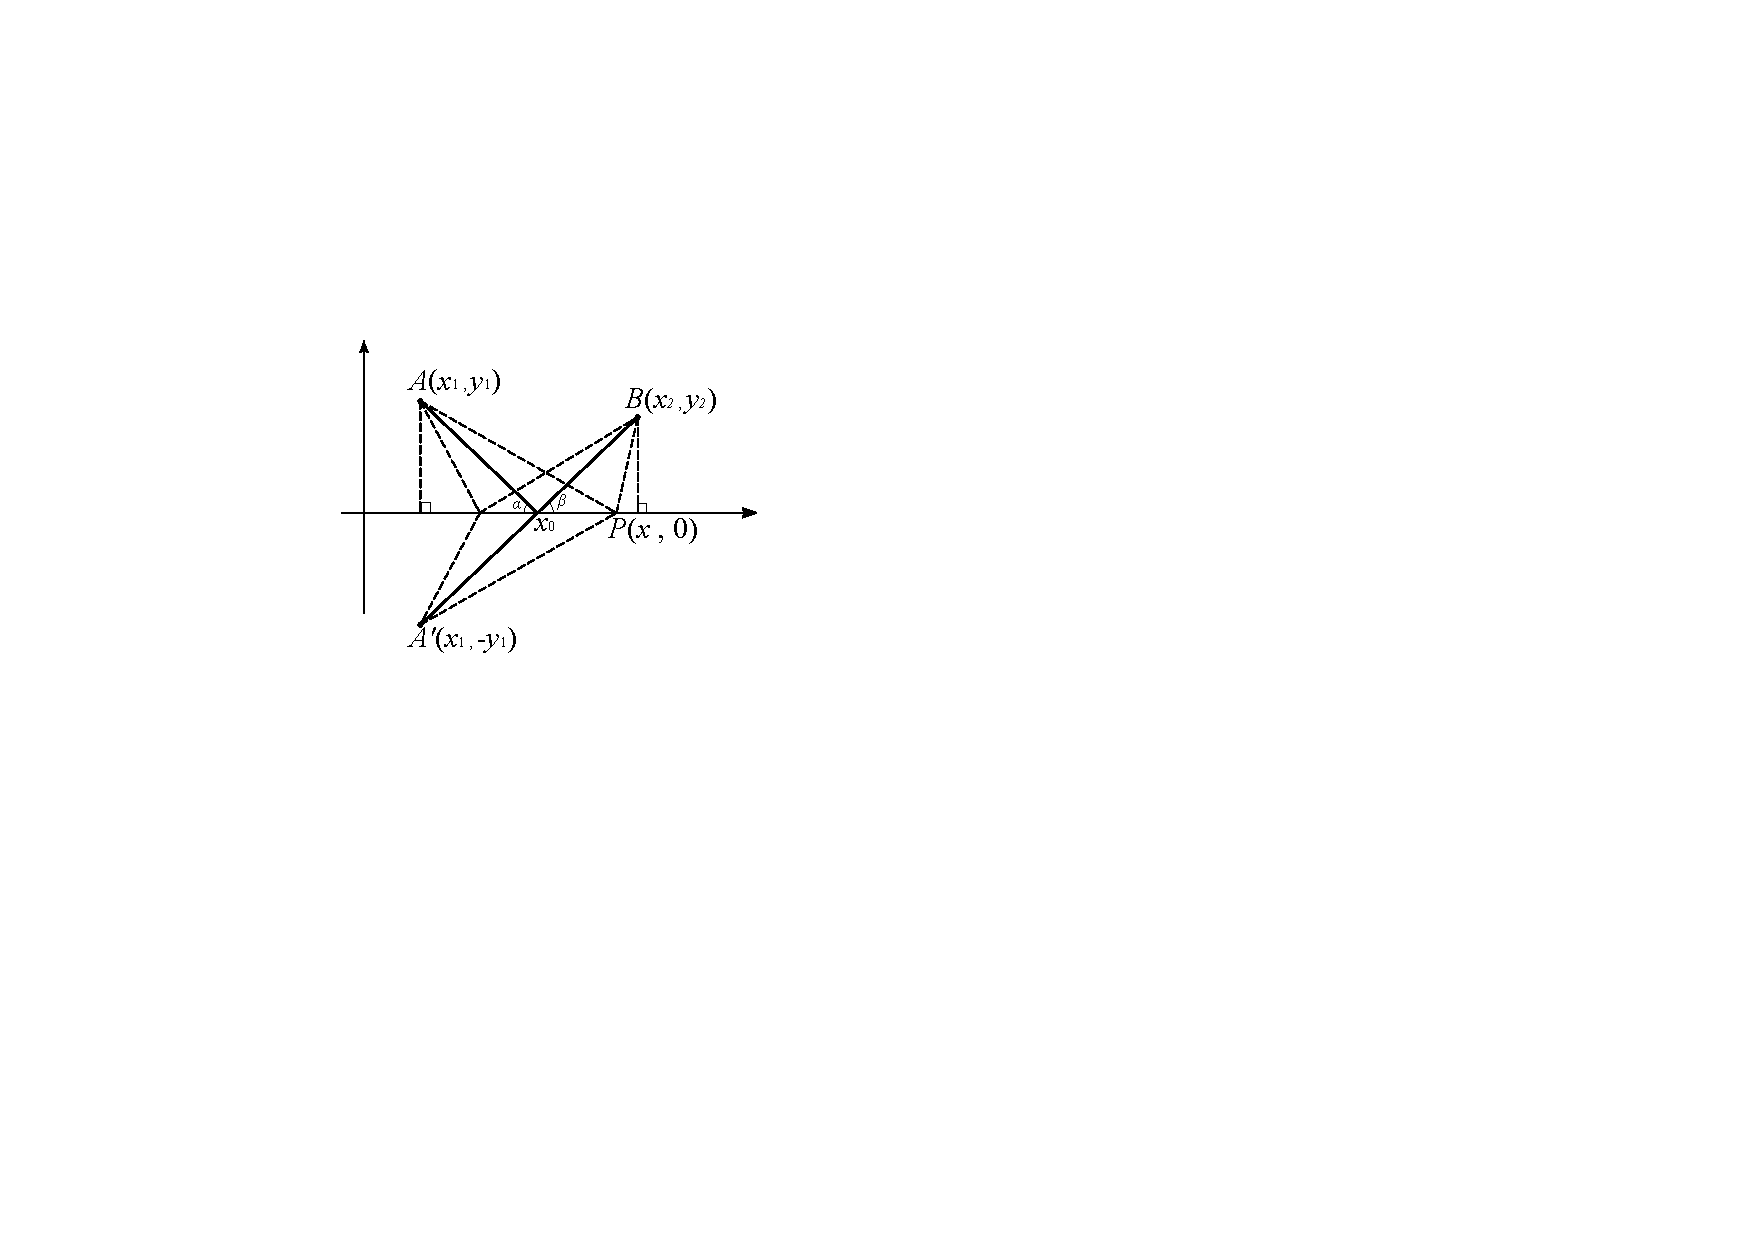
\includegraphics[width=0.5\linewidth]{反射定律}
\end{figure}  \\
\textbf{解}\ 作出点$ A(x_1,y_1) $关于$ x $轴的对称点
$ A'(x_1,-y_1) $,那么,
\begin{align*}
    |PA|+|PB|=|PA'|+|PB|\geq |A'B|=\sqrt{(x_2-x_1)^2+(y_2+y_1)^2}
\end{align*}
也可以直接求导:
\begin{gather*}
    f(x)=\sqrt{(x-x_1)^2+y_1^2}+\sqrt{(x-x_2)^2+y_2^2} \\
    f'(x)=\dfrac{x-x_1}{\sqrt{(x-x_1)^2+y_1^2}}+
    \dfrac{x-x_2}{\sqrt{(x-x_2)^2+y_2^2}}=0  \\
    \cos \alpha=\dfrac{x_0-x_1}{\sqrt{(x_0-x_1)^2+y_1^2}}=
    \dfrac{x_2-x_0}{\sqrt{(x_0-x_2)^2+y_2^2}} =\cos \beta
\end{gather*}
因为$ \alpha,\beta $都是锐角,所以$ \alpha=\beta $. 此时,
$ f(x) $取最小值$ |A'B| $.
这实际上就是光的反射定律:光线从光源$ A $出发到达目标点$ B $,
会走最短的路径,此时入射角等于反射角。

% xTb_log21Tx_Approx.m
\item\label{魔术数0x5f3759df}  
设$ b\in \textbf{R},\ E(b) $代表$ |x+b-\log_2(1+x)| $
在$ x\in[0,1] $时的最大值,
当$ b $为多少时,$ E(b) $取得最小值?\\
\textbf{解}\ 考虑直线$ y=x+b $以及对数函数$ y=\log_2(1+x) $
在$ [0,1] $上的图像,假想$ b $从$ -\infty $变化到$ +\infty $,
那么直线与对数曲线的交点数量将会依次为0,2,1,0,显然在交点数量
为2的时候,$ E(b) $才可能取得最小值。如下图,
\begin{figure}[h]
    \centering
    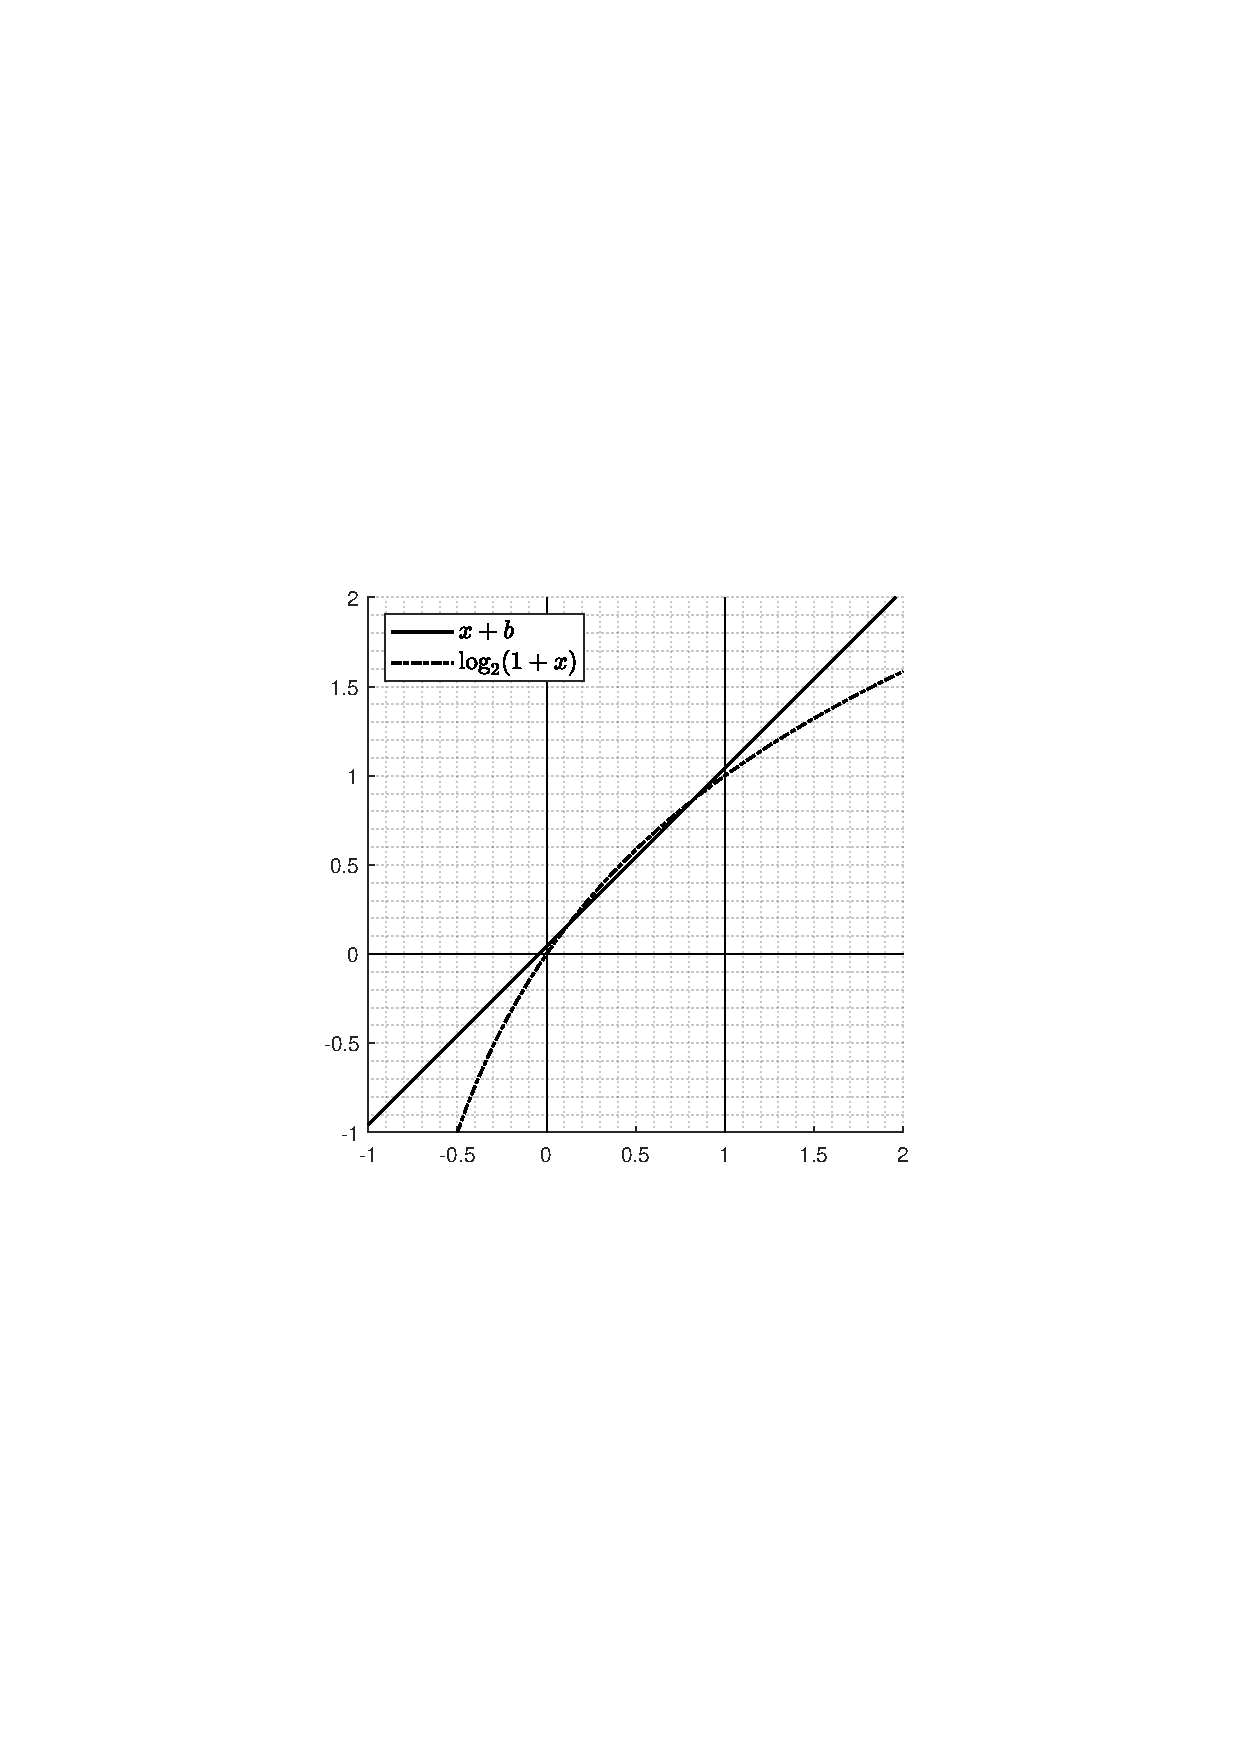
\includegraphics[width=0.5\linewidth]{PDF_Picture/x+b-log2(1+x)最大最小值}
\end{figure}
令$ f(x)=x+b-\log_2(1+x) $,则$ f(0)=b=f(1) $,
$ f'(x)=1-\dfrac{1}{(1+x)\ln2},\ f'\left(\dfrac{1}{\ln2}-1
\right)=0 $,
\begin{gather*}
    f\left(\dfrac{1}{\ln2}-1\right)=
    \dfrac{1}{\ln2}-1+b+\dfrac{\ln(\ln2)}{\ln2}<0
\end{gather*}
当$ b>0 $且$ f(0)=-f\left(\dfrac{1}{\ln2}-1\right)=f(1) $时,
$ E(b) $取得最小值,所以
\begin{gather*}
    -\left[\dfrac{1}{\ln2}-1+b+\dfrac{\ln(\ln2)}{\ln2}\right]=b\\
    b=\dfrac{1}{2}-\dfrac{1+\ln(\ln2)}{2\ln2}=0.043035666027967\cdots
\end{gather*}

\textbf{注}:以上面的$ b $为基础,再导出2个数字,下面出现了
23, 127, 52, 1023,这4个数字均来源于IEEE 754浮点数的规范。
\begin{gather*}
    \dfrac{3}{2}\times 2^{23}\times(127-b)=
    1597488310.001508\cdots
\end{gather*} 
最接近这个数的整数是1597488310,用16进制表示是5f37bcb6.
\begin{gather*}                
    \dfrac{3}{2}\times 2^{52}\times(1023-b)=
    6910482905085795321.358862\cdots              
\end{gather*}
最接近这个数的整数是6910482905085795321,
用16进制表示是5fe6f796c00c5bf9. 
我们将在\ref{无除法的平方根迭代算法}
看到这两个以5f开头的16进制数的作用。

\item 设$ a>0,b>0 $,函数$ f(x)=\e^{-ax} $与函数
$ g(x)=\e^{-ax}\cos(bx) $的交点的横坐标是多少?
这两个函数在交点处的导数值是否相等?\\
\textbf{解}\ 令$ f(x)=g(x) $,则$ \e^{-ax}=\e^{-ax}\cos(bx)
\Rightarrow \cos(bx)=1 $,$ bx=2k\pi\ (k\in\textbf{Z}) $,
$ x=\dfrac{2k\pi}{b} $,这就是交点的横坐标。 \\
$ f'(x)=-a\e^{-ax} $,$ g'(x)=-\e^{-ax}[a\cos(bx)+b\sin(bx)] $. \\ 
当$ \cos(bx)=1 $时,$ \sin(bx)=0 $,此时
$ f'(x)=g'(x)=-a\e^{-2ak\pi/b} $,两个函数在交点处的导数值相等,
这说明交点恰好是切点,但不是$ g(x) $的极值点(因为此时
$ a\cos(bx)+b\sin(bx)\neq 0 $.) \\
取$ a=0.1,\ b=1 $,此时$ f(x) $和$ g(x) $的图像如下:
\begin{figure}[H] % DampedFreeOscillation.m
    \centering
    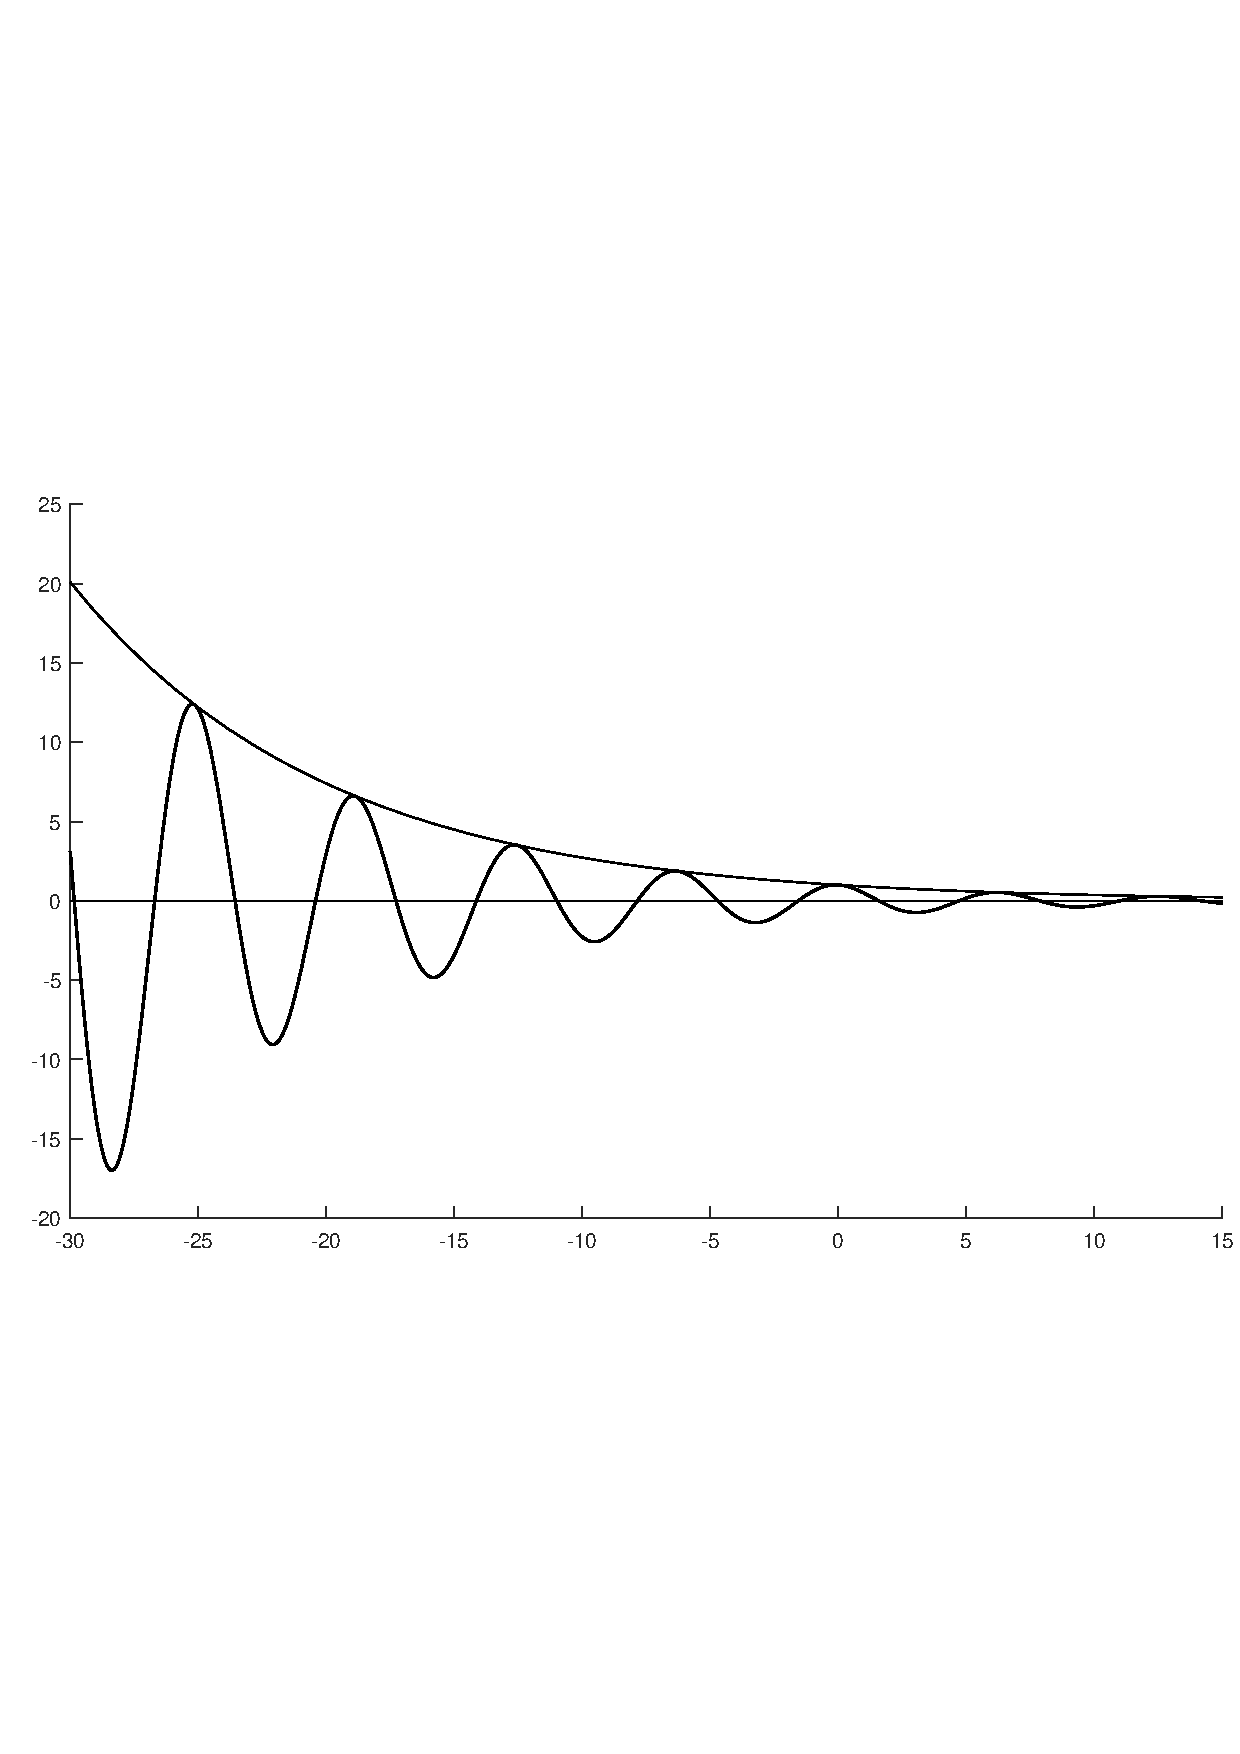
\includegraphics[width=0.8\linewidth]{PDF_Picture/有阻尼自由振荡函数图像}
\end{figure}
$ g(x) $经常被用来描述一些振幅随时间衰减的振荡现象,
比如一个弹簧挂着一个重物在空气中上下振荡,如果没有外界能量输入,
则空气阻力会导致振幅越来越小。

\item 曲线$y=f(x)$的曲率半径定义为
$\rho=\dfrac{(1+y'^2)^{3/2}}{|y''|}$,其中$y''$代表二阶导数,
或者说求两次导数。
那么指数函数$y=C\e^{ax}\ (C>0, a\neq 0)$的曲率半径在何处取最小值?\\
\textbf{解}\ $y'=Ca\e^{ax},\ y''=Ca^2\e^{ax}$,
\begin{align*}
    r =&\ \dfrac{(1+C^2a^2\e^{2ax})^{3/2}}{Ca^2\e^{ax}}  \\
    =&\ \left(\dfrac{1+C^2a^2\e^{2ax}}{C^{2/3}a^{4/3}\e^{2ax/3}}\right)^{3/2} \\
    =&\ \left(\dfrac{1}{2C^{2/3}a^{4/3}\e^{2ax/3}}+
    \dfrac{1}{2C^{2/3}a^{4/3}\e^{2ax/3}}+
    C^{4/3}a^{2/3}\e^{4ax/3}\right)^{3/2} \\
    \geq&\ \left[3\left(\dfrac{C^{4/3}a^{2/3}\e^{4ax/3}}{
        2C^{2/3}a^{4/3}\e^{2ax/3}\cdot 2C^{2/3}a^{4/3}\e^{2ax/3}}
    \right)^{1/3}\right]^{3/2} \\
    =&\ \left[3\left(\dfrac{1}{4a^2}\right)^{1/3}\right]^{3/2}
    =\dfrac{3\sqrt{3}}{2|a|}
\end{align*}
等号成立条件为$ \dfrac{1}{2C^{2/3}a^{4/3}\e^{2ax/3}}=
C^{4/3}a^{2/3}\e^{4ax/3} $,\\ 
即$2C^2a^2\e^{2ax}=1$,$x=-\dfrac{1}{a}\ln(\sqrt{2}Ca)$. 

\item 求证:$ \e^x-\ln x>2\ (x>0) $. \\
\textbf{解}\ 令$ f(x)=\e^x-\ln x $,则$ f'(x)=\e^x-\dfrac{1}{x} $,
令$ f'(x_0)=0 $可得$ \e^{x_0}=\dfrac{1}{x_0},\ x_0\e^{x_0}=1,\ 
\ln x_0+x_0=0 $,显然有$ 0<x_0<1 $,$ x_0 $是$ f(x) $的极小值点,于是,
\begin{align*}
    f(x)\geq f(x_0)=\e^{x_0}-\ln x_0=\e^{x_0}+x_0=\dfrac{1}{x_0}+x_0>2
\end{align*}
令$ W(x) $代表Lambert W函数($ y=xe^x $的反函数),则$ x_0=W(1)=0.567143\cdots $.
若不使用计算器,可按如下方法估计$ x_0 $的大小:
$ \e<4 ,\ \e^{1/2}< 2,\ \dfrac{1}{2}\e^{1/2} <1=x_0\e^{x_0} $,
所以$ \dfrac{1}{2}<x_0 $. 另外,
$ \e>2.56=1.6^2,\ \e^{x_0}>\e^{1/2}>1.6,\ f(x_0)=\e^{x_0}+x_0
>1.6+0.5=2.1 $. 实际上,$ f(x_0)=2.330366\cdots $. 

\item  设$ f(x)=x^3-2x+4,\ g(x)=\sqrt{x^3-2x+4} $,\\
(1) 设$ x_0 $满足$ f'(x_0)=g'(x_0) $,求$ x_0 $所满足的三次方程,
并借助计算器求出$x_0$的值,精确到小数点后2位。\\
(2) 从点$ P(4,0) $可以作出三次曲线$ y=g(x) $的若干条切线,求所有
切点的横坐标。\\
\textbf{解}\ $ f'(x)=3x^2-2,\ g'(x)=
\dfrac{\frac{1}{2}(3x^2-2)}{\sqrt{x^3-2x+4}} $,
令$ f'(x_0)=g'(x_0) $,有$ x_0^3-2x_0+\dfrac{15}{4}=0 $,
$x_0=-1.974614997\cdots $. \\
(2) 设切点为$ T(x,g(x)) $,则$ \dfrac{g(x)}{x-4}=g'(x) $,
\begin{gather*}
    \dfrac{\sqrt{x^3-2x+4}}{x-4}=
    \dfrac{\frac{3}{2}x^2-1}{\sqrt{x^3-2x+4}} \\
    \left(\frac{3}{2}x^2-1\right)(x-4)-(x^3-2x+4)=0 \\
    x(x^2-12x + 2)=0
\end{gather*}
所以,三个切点的横坐标依次为$ 6-\sqrt{34},\ 0,\ 6+\sqrt{34}$.

\item \label{四次函数的轴对称性}
若$ f(x)=x(x+1)(x^2+ax+b) $,且$ f(x) $的对称轴是$ x=
-\dfrac{3}{2} $,\\ (1)求$ a,b $;\quad (2)求$ f(x) $在$ \textbf{R} $
上的最小值。\\
\textbf{解}\ (1) 因为$ f(-1)=f(0)=0 $,由对称性必有$ f(-2)=f(-3)=0 $,
故$ x^2+ax+b=(x+2)(x+3)=x^2+5x+6,\ a=5,\ b=6 $. \\
(2) \textbf{方法一}
\begin{align}\label{x(x+1)(x+2)(x+3)}
    f(x)=[x(x+3)][(x+1)(x+2)]=&(x^2+3x)(x^2+3x+2) \\
    =&[(x^2+3x)+1]^2-1 \geq -1 
\end{align}
当$ x^2+3x+1=0 $,即 $ x=\dfrac{-3\pm\sqrt{5}}{2} $时,等号成立。\\
\eqref{x(x+1)(x+2)(x+3)}式中的因式分解的技巧性较强,事实上有更一般的
方法,即先将$ f(x) $展开成$ x^4 + 6x^3 + 11x^2 + 6x $,再令其等于
\begin{gather}\label{四次函数配成二次函数平方加常数}
    (x^2+cx+d)^2+g=x^4+2cx^3+(c^2+2d)x^2+2dcx+(d^2+g) 
\end{gather}
比较系数可得
$ \begin{cases}
    2c=6 \\
    c^2+2d=11 \\
    2dc=6 \\
    d^2+g=0
\end{cases} \Rightarrow 
\begin{cases}
    c=3 \\
    d=1\\
    g=-1
\end{cases} $. 当然,不是所有的4次函数都可以进行
\eqref{四次函数配成二次函数平方加常数}式这样的配方操作,比如
$ (x-1)(x-2)(x-3)(x-5)=x^4-11x^3+41x^2-61x+30 $就无法进行,
比较系数得到的方程会相互矛盾,
只有当四次函数的图像是轴对称图形时才可以进行。

\textbf{方法二}\ $ f(x)=x^4 + 6x^3 + 11x^2 + 6x,\ f'(x)=4x^3+18x^2+22x+6=
2(2x + 3)(x^2 + 3x + 1) $. 剩余步骤略。注意:$ f'(x) $的对称中心是
$ \left(-\dfrac{3}{2},0\right ) $,恰好在$ x $轴上。\\
\textbf{推广1}:若四次函数有4个实根$ x_1,x_2,x_3,x_4 $,
不妨设$ x_1\leq x_2\leq x_3\leq x_4 $. 
\begin{itemize}[itemsep=-1pt]
    \item 若$ x_1,x_2,x_3,x_4 $成等差数列,那么该函数存在对称轴
    $ x=\dfrac{x_1+x_4}{2}=\dfrac{x_2+x_3}{2} $. 
    \item 若$ x_1+x_4=x_2+x_3 $,那么该函数存在对称轴
    $ x=\dfrac{x_1+x_4}{2}=\dfrac{x_2+x_3}{2} $.
\end{itemize}
\textbf{推广2}:若四次函数的导函数的对称中心在$ x $轴上,
那么这个四次函数是轴对称图形,对称轴的横坐标就是导函数对称中心的横坐标。
从定积分的角度是很容易理解这一点的。

\item $^*$ 设$ \i $是虚数单位,$ z=x+y\i $,
对于下面定义的$ u(x,y),\ v(x,y) $,
证明:$ \begin{cases}
    \dfrac{\partial u}{\partial x} =\dfrac{\partial v}{\partial y} \\
    \dfrac{\partial v}{\partial x} =-\dfrac{\partial u}{\partial y} 
\end{cases} $. (这两个等式被称为柯西-黎曼条件,或C-R条件。)\\
(1)\ $ z^2=(x+y\i)^2=x^2-y^2+2xy\i,\ u(x,y)=x^2-y^2,\ v(x,y)=2xy $; \\
(2)\ $ z^3=(x+y\i)^3=x^3-3xy^2+(3x^2y-y^3)\i,\ u(x,y)=x^3-3xy^2,\ 
v(x,y)=3x^2y-y^3 $; \\
(3)\ $ \ln z=\ln(x+y\i)=\dfrac{1}{2}\ln(x^2+y^2)+\left(\arctan\dfrac{y}{x}\right)\i,
\ u(x,y)=\dfrac{1}{2}\ln(x^2+y^2),\ v(x,y)=\arctan\dfrac{y}{x} $; 
(注:$ (\arctan x)'=\dfrac{1}{1+x^2} $). \\
\textbf{解}\ (1) $ \dfrac{\partial u}{\partial x} =2x=
\dfrac{\partial v}{\partial y} $,
$ \dfrac{\partial v}{\partial x} =2y=
-\dfrac{\partial u}{\partial y} $. \\
(2) $ \dfrac{\partial u}{\partial x} =3x^2-3y^2=
\dfrac{\partial v}{\partial y} $,
$ \dfrac{\partial v}{\partial x} =6xy=
-\dfrac{\partial u}{\partial y} $. \\
(3) $ \dfrac{\partial u}{\partial x} =\dfrac{x}{x^2+y^2}=
\dfrac{\partial v}{\partial y} $,
$ \dfrac{\partial v}{\partial x} = -\dfrac{y}{x^2+y^2}=
-\dfrac{\partial u}{\partial y} $. \\
\textbf{注}:以上每一小问中定义的$ u(x,y),\ v(x,y) $,
实际上就是一个复变函数的实部和虚部。

\item (2011,四川高考,理)求证:$ \dfrac{2}{3}n^{3/2}<\sum\limits_{k=1}^{n}\sqrt{k}<
\dfrac{2}{3}n^{3/2}+\dfrac{1}{2}n^{1/2} $. \\
\textbf{证}\ $ n=1 $时,原不等式显然成立。考虑$ n\geq 2 $,采用逆向分析法(倒推法、执果索因法)
\begin{gather*}
    \dfrac{2}{3}n^{3/2}-\dfrac{2}{3}(n-1)^{3/2}<\sqrt{n}<
    \dfrac{2}{3}n^{3/2}-\dfrac{2}{3}(n-1)^{3/2}+\dfrac{1}{2}n^{1/2}
    -\dfrac{1}{2}(n-1)^{1/2} \\
    \dfrac{2}{3}(\sqrt{n}-\sqrt{n-1})(n+\sqrt{n(n-1)}+n-1)<\sqrt{n}< \\
    \dfrac{2}{3}(\sqrt{n}-\sqrt{n-1})(n+\sqrt{n(n-1)}+n-1)+
    \dfrac{1}{2}(\sqrt{n}-\sqrt{n-1}) 
\end{gather*}
上式全部乘$ 3(\sqrt{n}+\sqrt{n-1}) $,可得:
\begin{gather*}
    2\left(2n-1+\sqrt{n(n-1)}\right)<3n+3\sqrt{n(n-1)}<
    2\left(2n-1+\sqrt{n(n-1)}\right)+\dfrac{3}{2} 
\end{gather*}
上式全部减去$ 3n+2\sqrt{n(n-1)} $,可得:
\begin{gather*}
    n-2< \sqrt{n(n-1)}<n-\dfrac{1}{2} \\
    n^2-4n+4<n^2-n<n^2-n+\dfrac{1}{4}
\end{gather*}
显然成立。同样的方法可以证明:
\begin{gather*}
    \dfrac{2}{3}n^{3/2}+\dfrac{1}{3}n^{1/2}\leq\sum\limits_{k=1}^{n}\sqrt{k}
    \leq \dfrac{2}{3}n^{3/2}+\dfrac{1}{2}n^{1/2}-\dfrac{1}{6} 
\end{gather*}
本题显然是以(\ref{0.5次方求和})式为背景。另外,还有更强的结论:
\begin{gather*}
    \dfrac{2}{3}n^{3/2}+\dfrac{1}{2}n^{1/2}
    \underbrace{-\dfrac{5}{24}}_{\approx -0.2083}
    <\dfrac{2}{3}n^{3/2}+\dfrac{1}{2}n^{1/2}+
    \underbrace{\zeta\left(-\dfrac{1}{2}\right)}_{\approx -0.2079}  
    < \sum\limits_{k=1}^{n} \sqrt{k}\leq \dfrac{2}{3}n^{3/2}
    +\dfrac{1}{2}n^{1/2}-\dfrac{1}{6} 
\end{gather*}

\item (2013,湖北高考,理)设$ n $是正整数,$ r $为正有理数。\\
(I)求函数$ f(x)=(1+x)^{r+1}-(r+1)x-1\ (x>-1) $的最小值;\\
(II)证明:$ \dfrac{n^{r+1}-(n-1)^{r+1}}{r+1}<n^r<
\dfrac{(n+1)^{r+1}-n^{r+1}}{r+1} $. \\ 
(III)设$ x\in \textbf{R} $,记$ \lceil x \rceil $为不小于$ x $的最小整数,
例如,$ \lceil 2 \rceil=2,\ \lceil \pi \rceil=4,\ \lceil -\dfrac{3}{2}
\rceil=-1 $,记$ S=\sqrt[3]{81}+\sqrt[3]{82}+\cdots +\sqrt[3]{125} $,
求$ \lceil S \rceil $的值。(参考数据:$ 80^{4/3}\approx 344.7,\ 
81^{4/3}\approx 350.5,\ 124^{4/3}\approx 618.3,
\ 126^{4/3}\approx 631.7 $).\\
\textbf{解}\ (I) $ f'(x)=(r+1)(1+x)^r-(r+1)=(r+1)[(1+x)^r-1],\ f'(0)=0 $,$ f(x) $
在$ x=0 $处取得最小值0. 事实上,$ y=(r+1)x+1 $就是$ y=(1+x)^{r+1} $
在$ x=0 $处的切线,$ (1+x)^{r+1}\geq (r+1)x+1 $,等号仅在$ x=0 $处成立。\\
(II) 取$ x=\dfrac{1}{n} $,则$ f(\dfrac{1}{n})=\left(1+
\dfrac{1}{n}\right)^{r+1}-\dfrac{r+1}{n}-1>0 $,即得$ n^r<
\dfrac{(n+1)^{r+1}-n^{r+1}}{r+1} $. 再取$ x=-\dfrac{1}{n},\ 
f(-\dfrac{1}{n})>0 $,
(这里假设$ n\geq 2 $,因为$ n=1 $时,$ \dfrac{1}{r+1}<1 $显然成立。)
可得$ \dfrac{n^{r+1}-(n-1)^{r+1}}{r+1}<n^r $. \\
(III)在(II)中的不等式中,取$ r=\dfrac{1}{3} $,然后依次取$ n=81,82,\cdots,
125 $,将这些不等式全部相加可得:
\begin{gather*}
    \dfrac{125^{4/3}-80^{4/3}}{4/3}<S<\dfrac{126^{4/3}-81^{4/3}}{4/3} \\
    \dfrac{3}{4}(625-344.7)=210.225<S<\dfrac{3}{4}(631.7-350.5)=210.9
\end{gather*}
所以,$ \lceil S \rceil =211 $. \\
\textbf{注} (II)中的不等式,从定积分的角度来看是显然的。
\begin{gather*}
    \dfrac{n^{r+1}-(n-1)^{r+1}}{r+1}=\int_{n-1}^n x^r \d x<n^r<
    \int_{n}^{n+1} x^r \d x=\dfrac{(n+1)^{r+1}-n^{r+1}}{r+1}
\end{gather*}
对于第(III)问,$ \lceil x \rceil $也被称为向上取整,借助软件可算出$ S $
的精确值为$ 210.5630174850639 \cdots $,本小问其实就是以
(\ref{三分之一次方求和})式为背景,也可以说是以“用定积分估计求和”为背景。 \\
\mycircled{1} 采用(\ref{三分之一次方求和})式进行估计:
\begin{align*}
    \dfrac{3}{4}\cdot 125^{4/3}+\dfrac{1}{2}\cdot 125^{1/3}-\dfrac{1}{4}-
    \left(\dfrac{3}{4}\cdot 80^{4/3}+\dfrac{1}{2}\cdot 80^{1/3}-\dfrac{1}{4} \right) 
    =210.563403\cdots
\end{align*}
如果不使用计算器,就需要用前面讲过的开三次方的方法对$ \sqrt[3]{80} $
进行估算\footnote{\q $ \sqrt[3]{80}=4.308869380063767\cdots $},
$ 4^3=64<80<5^3=125 $,采用迭代法(反复使用切线法),
$ a_0=4,\ a_1=\dfrac{1}{3}(2a_0+
\dfrac{80}{a_0^2})=\dfrac{13}{3}=4.333\cdots,\ a_1=\dfrac{1}{3}(2a_1+
\dfrac{80}{a_1^2})=\dfrac{6554}{1521}=4.309007\cdots $,
误差已经小于万分之二。最笨的方法就是通过计算$ 4.1^3,
\ 4.2^3,\ 4.3^3,\ 4.4^3\cdots $来进行估计。如果对此题进行修改,
改成从$ \sqrt[3]{65} $连加到$ \sqrt[3]{125} $,
没有改变问题的本质,但会变得更加优美,使用方法\mycircled{1}时,
便无需计算$ \sqrt[3]{80} $,即
\begin{align*}
    &\ \sqrt[3]{65}+\sqrt[3]{66}+\cdots+\sqrt[3]{125}
    \quad (\text{求和精确值为}277.249375006532\cdots)\\
    \approx &\ \dfrac{3}{4}\cdot 125^{4/3}+\dfrac{1}{2}\cdot 125^{1/3}-\dfrac{1}{4}-
    \left(\dfrac{3}{4}\cdot 64^{4/3}+\dfrac{1}{2}\cdot 64^{1/3}-\dfrac{1}{4} \right) 
    =\dfrac{1109}{4}=277.25
\end{align*}
\mycircled{2}直接对两个定积分求平均值:
\begin{align*}
    &\dfrac{1}{2}\left(\int_{80}^{125}x^{1/3}\d x+\int_{81}^{126}x^{1/3}\d x \right) \\
    =&\dfrac{1}{2}\cdot \dfrac{3}{4}\left( 125^{4/3} -80^{4/3}+126^{4/3}-
    81^{4/3} \right)= 210.562253 \cdots
\end{align*}
这就是高考标准答案中的$ 210.225 $和$ 210.9 $的平均值。\\
\mycircled{3}积分起点和终点改到整数点的中点:
\begin{align*}
    \int_{80.5}^{125.5}x^{1/3}\d x=
    \dfrac{3}{4}\left(125.5^{4/3} - 80.5^{4/3}\right) =210.562826 \cdots
\end{align*}
第\mycircled{1}种估算$ S $的方法精度最高。

\item $ ^* $求证:$ \forall n\in \textbf{N}^+,\ n\geq 2 $,$ \sum\limits_{k=2}^{n} 
k\ln k<\dfrac{1}{2}(n+1)^2\Big[\ln(n+1)-\dfrac{1}{2} \Big]-1 $. \\
(已知$ \ln 2\approx 0.693147,\ \ln 3\approx 1.098612 $.) \\
\textbf{证}\ $ n=2 $ 时,$ 2\ln 2<\dfrac{9}{2}\Big[\ln 3-
\dfrac{1}{2}\Big]-1\approx 1.693755 $. 当$ n\geq 3 $时,
只需要证明
\begin{gather*}
    n\ln n<\dfrac{1}{2}(n+1)^2\Big[\ln(n+1)-\dfrac{1}{2} 
    \Big]-\dfrac{1}{2}n^2\Big[\ln n-\dfrac{1}{2} \Big] 
\end{gather*}
令$ f(x)=\dfrac{1}{2}(x+1)^2\Big[\ln(x+1)-\dfrac{1}{2} 
\Big]-\dfrac{1}{2}x^2\Big[\ln x-\dfrac{1}{2} \Big]-x\ln x\ 
(x\geq 3) $,
则
\begin{align*}
    f'(x) =(x+1)\ln(x+1)-x\ln x-\ln x-1 &=
    (x+1)\ln\Big(1+\frac{1}{x}\Big)-1\\
    &=(x+1)\Big[\ln\Big(1+\frac{1}{x}\Big)-\frac{1}{x+1}\Big]
\end{align*}
利用拉格朗日中值定理:
\begin{gather*}
    \dfrac{1}{x+1}<\dfrac{\ln(x+1)-\ln x}{(x+1)-x}<\dfrac{1}{x}
\end{gather*}
可得$ f'(x)>0 $. 或者继续求导,
\begin{align*}
    f''(x)=\ln\Big(1+\frac{1}{x}\Big)-\frac{1}{x}<0
\end{align*}
因为$ \lim\limits_{x\to+\infty}f'(x)=\lim\limits_{x\to+\infty}
\ln\Big(1+\dfrac{1}{x}\Big)^{x+1}-1=\ln \e-1=0 $,
所以,$ f'(x)>f'(+\infty)=0 $,$ f(x) $在$ (3,+\infty) $
上单调递增,$ f(x)\geq f(3)\approx 1.100762>0 $。证毕。\\
\textbf{注1}:此题的命制背景显然是:
\begin{align*}
    \sum\limits_{k=2}^{n} k\ln k<\int_2^{n+1}x\ln x\d x &=
    \left.\dfrac{1}{2}x^2\Big(\ln x-\dfrac{1}{2}\Big)\right|_2^{n+1} \\
    &=\dfrac{1}{2}(n+1)^2\Big[\ln(n+1)-\dfrac{1}{2} \Big]
    -\underbrace{\dfrac{1}{2}\cdot2^2\Big[\ln 2-\dfrac{1}{2} 
        \Big]}_{\approx 0.386294 }
\end{align*}
\textbf{注2}:设$  n\in \textbf{N}^+,\ n\geq 1 $,定义
\begin{gather*}
    F_n(x)=\frac{1}{n}(x+1)^{n+1}\Big[\ln (x+1)-\frac{1}{n}\Big]
    -\frac{1}{n}x^{n+1}\Big(\ln x-\frac{1}{n}\Big)-x^{n-1}\ln x
\end{gather*}
则
\begin{gather*}
    [F_n(x)]^{(n-1)}=(n-1)!F_1(x)
    =(n-1)!\Big[(x+1)\ln\Big(1+\frac{1}{x}\Big)-1\Big]
\end{gather*}
感兴趣的读者自行完成证明。可以使用两函数之积的高阶导数的莱布尼茨公式直接证明,
也可以使用数学归纳法证明,注意如下规律,
\begin{align*}
    F_{n+1}'(x)+x^{n-1} & =(x+1)^n\ln(x+1)-x^n\ln x-nx^{n-1}\ln x\\
    & =nF_n(x)+\dfrac{1}{n}[(x+1)^n-x^n]
\end{align*}
\textbf{注3}:尝试只用导数而不用积分,证明以下两个不等式(会遇到一些困难),\\
(1)\ $ n\in \textbf{N}^+,\ n\geq 2 $,$ \sum\limits_{k=2}^{n}
\dfrac{1}{k\ln k}<\ln(\ln (n+1))+0.8 $.\\ 
(2)\ $ n\in \textbf{N}^+,\ n\geq 2 $,$ \sum\limits_{k=2}^{n}
\dfrac{\ln k}{k}<\dfrac{1}{2}[\ln(n+1)]^2 $.

\item (2022,新高考II卷)已知函数$f(x)=x\mathrm{e}^{ax}-\mathrm{e}^{x}$. \\
(I)当$a=1$时,讨论$f(x)$的单调性;\\
(II)当$x>0$时,$f(x)<-1$,求实数$ a $的取值范围;\\
(III)设$n\in\mathbf{N}^+$,证明:$\dfrac{1}{\sqrt{1^{2}+1}}+
\dfrac{1}{\sqrt{2^{2}+2}}+\cdots+\dfrac{1}{\sqrt{n^{2}+n}}>\ln(n+1)$. \\
\textbf{解}\ (I) 当$a=1$时,$ f'(x)=x\e^x $,$ f(x) $
在$ (-\infty,0) $上单调递减,在$ (0,+\infty) $上单调递增。\\
(II) 
\begin{align*}
    & f'(x)=(1+ax)\e^{ax}-\e^x,\q f'(0)=0 \\
    & f''(x)=(2a+a^2x)\e^{ax}-\e^x,\q f''(0)=2a-1
\end{align*}
\mycircled{1} 若$ f''(0)=2a-1\leq 0,\ a\leq \dfrac{1}{2} $,则$ x=0 $
是$ f(x) $的一个极大值点,且
\begin{align*}
    f'(x) &=(1+ax)\e^{ax}-\e^x\\ &\leq \left(1+\dfrac{1}{2}x\right)
    \e^{\frac{x}{2}}-\e^x=\e^{\frac{x}{2}}\left(1+\dfrac{x}{2}-
    \e^{\frac{x}{2}}\right)<0 \q (x>0)
\end{align*}
所以,$ f(x)<f(0)=-1 $. \\
\mycircled{2} 若$ a>\dfrac{1}{2} $,则$ f''(0)=2a-1>0 $,
必存在$ x_0>0 $,使得当$ x\in(0,x_0) $时,$ f'(x)>f'(0)=0 $,
从而$ f(x)>f(0)=-1 $,不符合题意。\\
因此,$ a $的范围是$ \left(-\infty,\dfrac{1}{2}\right] $. \\
(III) \textbf{方法一}\ 令$ a=\dfrac{1}{2} $,由(II)可得
$ x\e^{\frac{x}{2}}-\e^x<-1 $,$ x<\e^{\frac{x}{2}}-\e^{-\frac{x}{2}} $,
令$ t=\e^{\frac{x}{2}}>1 $,则有$ 2\ln t<t-\dfrac{1}{t} $,
令$ t=\sqrt{\dfrac{n+1}{n}} $,则有
\begin{gather*}
    \ln \dfrac{n+1}{n}<\sqrt{\dfrac{n+1}{n}}-\sqrt{\dfrac{n}{n+1}}
    =\dfrac{1}{\sqrt{n^2+n}} \\
    \sum_{k=1}^{n}\dfrac{1}{\sqrt{k^2+k}}>
    \sum_{k=1}^{n}\ln \dfrac{k+1}{k}=\ln(n+1)
\end{gather*}
\textbf{方法二}\ 
\begin{gather*}
    \ln \dfrac{n+1}{n}<\ln \dfrac{n+2}{n+1}=
    \ln\left(1+\dfrac{1}{n+1}\right)<\dfrac{1}{n+1}<
    \dfrac{1}{\sqrt{n^2+n}}  
\end{gather*}
\textbf{方法三}\ 令$ g(x)=\ln\left(1+\dfrac{1}{x}\right)-
\dfrac{1}{\sqrt{x^2+x}} $,则
$ g'(x)=\dfrac{x+\frac{1}{2}-\sqrt{x^2+x}}{(x^2+x)\sqrt{x^2+x}}>0 $,
因为$ \lim\limits_{x\to+\infty}g(x)=0 $,所以$ g(x)<0\ (x>0) $. \\
\textbf{注1}:如果第(III)问直接使用分离变量法,
$ a<\dfrac{1}{x}\ln\dfrac{\e^x-1}{x}\ (x>0) $,右侧的函数
手工分析单调性很困难,但用软件可以证明它
在$ (0,+\infty) $上单调递增,利用$ \e^x $和$ \ln(1+x) $
在$ x=0 $处的泰勒级数求右侧函数在$ x\to 0 $时的极限。
\begin{align*}
    \lim_{x\to 0} \dfrac{1}{x}\ln\dfrac{\e^x-1}{x}  &=
    \lim_{x\to 0} \dfrac{1}{x}\ln\dfrac{x+
        \frac{1}{2}x^2+\frac{1}{6}x^3+\cdots}{x}\\ &=
    \lim_{x\to 0} \dfrac{1}{x}\ln\left(1+
    \frac{1}{2}x+\frac{1}{6}x^2+\cdots\right)\\ &=\lim_{x\to 0} 
    \dfrac{1}{x}\left(\frac{1}{2}x+\frac{1}{6}x^2+\cdots\right) 
    =\lim_{x\to 0}\left(\frac{1}{2}+\frac{1}{6}x+\cdots\right)
    =\dfrac{1}{2}
\end{align*}
\textbf{注2}:如果第(III)问直接使用积分比较法,
\begin{gather*}
    \int \dfrac{\d x}{\sqrt{x^2+b}}=\ln(x+\sqrt{x^2+b})+C \\
    \int \dfrac{\d x}{\sqrt{x^2+x}}=
    \int \dfrac{\d x}{\sqrt{\left(x+\frac{1}{2}\right)^2-\frac{1}{4}}}=
    \ln\left(x+\dfrac{1}{2}+\sqrt{x^2+x}\right)+C   
\end{gather*}
\begin{align*}
    \sum_{k=1}^{n}\dfrac{1}{\sqrt{k^2+k}} &>
    \int_1^{n+1}\dfrac{\d x}{\sqrt{x^2+x}} =
    \left.\ln\left(x+\dfrac{1}{2}+\sqrt{x^2+x}\right)\right|_1^{n+1} \\
    & =\ln\left(n+\dfrac{3}{2}+\sqrt{n^2+3n+2}\right)-
    \ln\left(\dfrac{3}{2}+\sqrt{2}\right)<\ln(1+n)
\end{align*}
最后一个不等号与需要的方向相反,除非把积分起点后移,否则做不出来。
但把积分起点后移会遇到十分麻烦的数字,所以本题不适合使用积分比较法。

\item 求证:$ \sqrt{1^4+1}+\sqrt{2^4+1}+\cdots+\sqrt{n^4+1}<\dfrac{n^3}{3}+\dfrac{n^2}{2}+
\dfrac{n}{6}+1 ,\ n\in \textbf{N}^+ $. \\
\textbf{证}\ $ y=\sqrt{1+x} $在$ x=0 $处的切线是$ y=1+\dfrac{x}{2} $,所以,当$ x>0 $时,
$ \sqrt{1+x}<1+\dfrac{x}{2} $,$ \sqrt{n^4+1}=n^2\sqrt{1+\dfrac{1}{n^4}}
<n^2\left(1+\dfrac{1}{2\cdot n^4}\right)=n^2+\dfrac{1}{2n^2} $,于是,
\begin{align*}
    &\sqrt{1^4+1}+\sqrt{2^4+1}+\cdots+\sqrt{n^4+1} \\
    <& 1^2+\dfrac{1}{2\cdot 1^2}+2^2+\dfrac{1}{2\cdot 2^2} +\cdots + n^2+\dfrac{1}{2n^2} \\
    <& \dfrac{n^3}{3}+\dfrac{n^2}{2}+\dfrac{n}{6}+\dfrac{1}{2}\left[\dfrac{1}{(1-\frac{1}{2})(1+\frac{1}{2})}+\dfrac{1}{(2-\frac{1}{2})(2+\frac{1}{2})}
    +\cdots+\dfrac{1}{(n-\frac{1}{2})(n+\frac{1}{2})}\right] \\
    <& \dfrac{n^3}{3}+\dfrac{n^2}{2}+\dfrac{n}{6}+1
\end{align*}
所以,原不等式成立。事实上,$ \sum\limits_{n=1}^{\infty}\dfrac{1}{n^2}=
\dfrac{\pi^2}{6} $,所以,最后的常数1还可以改进成$ \dfrac{\pi^2}{12}=0.822467\cdots $.

类似地可以证明:
\begin{align}
    \sqrt{4^1+1}+\sqrt{4^2+1}+\cdots+\sqrt{4^n+1}<&\ 2^{n+1}-\dfrac{3}{2} 
    \label{sqrt(4n+1)不等式}   \\
    \ln(\e^1+1)+\ln(\e^2+1)+\cdots+\ln(\e^n+1)<&\ \dfrac{n(n+1)}{2}+\dfrac{1}{\e-1}    \label{ln(en+1)不等式} 
\end{align}

提示:对(\ref{sqrt(4n+1)不等式})式,第一项$ \sqrt{5}=2.236\cdots<
\dfrac{9}{4}=2.25 $,从第二项开始使用不等式
$ \sqrt{4^n+1}<2^n+\dfrac{1}{2\cdot 2^n} $. 
对(\ref{ln(en+1)不等式})式,$ \ln(\e^n+1)=\ln \e^n+
\ln(1+\dfrac{1}{\e^n})<n+\dfrac{1}{\e^n} $. 

\item $ ^* $ 函数$ f(x) $的定义域为$ (0,+\infty) $,且恒满足$ f(x)>0,\ 2f(x)<xf'(x)<3f(x) $,则$ \dfrac{f(1)}{f(2)} $的范围是\underline{\hspace{2cm}}.\\
$ A.(\dfrac{1}{4},\dfrac{1}{2})\hspace{2cm} 
  B.(\dfrac{1}{16},\dfrac{1}{8})\hspace{2cm} 
  C.(\dfrac{1}{3},\dfrac{1}{2})\hspace{2cm} 
  D.(\dfrac{1}{8},\dfrac{1}{4})  $ \medskip \\
\textbf{方法一}\ $ \left[\dfrac{f(x)}{x^n}\right]'=
\dfrac{xf'(x)-nf(x)}{x^{n+1}} $,
\begin{gather*}
  \left[\dfrac{f(x)}{x^2}\right]'=\dfrac{xf'(x)-2f(x)}{x^{3}}>0,\q \left[\dfrac{f(x)}{x^3}\right]'=\dfrac{xf'(x)-3f(x)}{x^{4}}<0
\end{gather*}
所以$ \dfrac{f(1)}{1^2}>\dfrac{f(2)}{2^2},\ 
\dfrac{f(1)}{1^3}>\dfrac{f(2)}{2^3},\
\dfrac{1}{4}<\dfrac{f(1)}{f(2)}<\dfrac{1}{8} $.\\
\textbf{方法二}\ $ [\ln f(x)]'
=\dfrac{f'(x)}{f(x)} $,$ 2f(x)<xf'(x),\ \dfrac{2}{x}
<\dfrac{f'(x)}{f(x)}=[\ln f(x)]' $,
\begin{gather*}
	\int_1^t \dfrac{2}{x}\d x= 2\ln t-2\ln 1<
	\int_1^t [\ln f(x)]'\d x=\ln f(t)-\ln f(1)=
	\ln\dfrac{f(t)}{f(1)} \quad (t>1)
\end{gather*}
所以$ t^2<\dfrac{f(t)}{f(1)} $.同理可得$ \dfrac{f(t)}
{f(1)}<t^3 $,令$ t=2 $可得:$ 2^2<\dfrac{f(2)}{f(1)}<2^3 ,\ \dfrac{1}{4}<\dfrac{f(1)}{f(2)}<\dfrac{1}{8} $.\\
\textbf{注}:此题具有微分方程的背景,有的重点高中的模拟题中还出现了$ xf'(x)-f(x)=x\ln x $和$ xf'(x)+f(x)=\dfrac{\ln x}{x} $之类的微分方程。对于前者,两边同除$ x^2 $可化为:
\begin{gather*}
    \dfrac{xf'(x)-f(x)}{x^2}=\left[\dfrac{f(x)}{x}\right]'= \dfrac{\ln x}{x}=\left[\dfrac{1}{2}(\ln x)^2+C\right]'
\end{gather*}
所以$ f(x)=\dfrac{x}{2}(\ln x)^2+Cx $.对于后者,
\begin{gather*}
    xf'(x)+f(x)=[xf(x)]'=\dfrac{\ln x}{x}=
    \left[\dfrac{1}{2}(\ln x)^2+C\right]'
\end{gather*}
所以$ f(x)=\dfrac{1}{2x}(\ln x)^2+\dfrac{C}{x} $,其中$ C $为积分常数,
通常由$ f(x) $经过的某一点的坐标来确定。

\item \label{证明e^2x<(1+x)/(1-x)}  $ x\in (0,1) $,
证明$  \e^{2x}<\dfrac{1+x}{1-x} $. (即(\ref{exp(2x)帕德逼近})式,
本质是Pade逼近。) \\
\textbf{方法一}\ 当$ x\neq 0 $时,$ \e^x>1+x,\e^{-x}>1-x $,
当$ x \in (0, 1) $时,$ \e^x<\dfrac{1}{1-x} $,记$ f(x)=\e^{2x}-\dfrac{1+x}{1-x} $,则
\begin{align*}
    f'(x)=2\e^{2x}-\dfrac{2}{(1-x)^2}=
    2\left(\e^x+\dfrac{1}{1-x}\right)\left(\e^x-\dfrac{1}{1-x}\right)< 0
\end{align*}
所以,$ f(x)<f(0)=0 $. \\
\textbf{方法二}\ $ g(x)=\e^{2x}(1-x)-(1+x),\ g'(x)=(1-2x)\e^{2x}-1,\ g''(x)=-4x\e^{2x}<0,
\ g'(x)<g'(0)=0,\ g(x)<g(0)=0 $.即使不求二阶导数也能分析$ g'(x) $的正负,
当$ x\geq \dfrac{1}{2} $时,$ g'(x) $显然为负;
当$ 0< x<\dfrac{1}{2} $时,有$ \e^{2x}<\dfrac{1}{1-2x} $,
\begin{gather*}
    g'(x)=(1-2x)\e^{2x}-1=(1-2x)\left(\e^{2x}-\dfrac{1}{1-2x}\right)<0
\end{gather*}
\textbf{方法三}$ ^* $比较幂级数系数,把(\ref{ex泰勒展开})式中的$ x $换成$ 2x $:
\begin{align*}
    \e^{2x}=&\ 1+(2x)+\dfrac{(2x)^2}{2!}+\dfrac{(2x)^3}{3!}+\cdots + \dfrac{(2x)^n}{n!} +\cdots \\
     =&\ 1+2x+2x^2+\frac{4}{3}x^3+\cdots+\frac{2^n}{n!}x^n+\cdots \\
    \dfrac{1+x}{1-x}=-1+\dfrac{2}{1-x} 
    =&\ -1+2(1+x+x^2+x^3+\cdots + x^n +\cdots ) \\
    =&\ 1+2x+2x^2+2x^3+\cdots + 2x^n+\cdots 
\end{align*}
\textbf{方法四}$ ^* $当$ u \in (0,1) $时,$ 1<\e^u<\dfrac{1}{1-u} $,平方可得$ \e^{2u}<\dfrac{1}{(1-u)^2} $,然后在$ [0,x] $上积分,其中$ x\in (0,1) $,
\begin{align*}
    \int_{0}^{x}\e^{2u}\d u &<\int_{0}^{x}\dfrac{\d u}{(1-u)^2}\\  
    \left.\dfrac{1}{2}\e^{2u}\right|_0^x
    =\dfrac{1}{2}(\e^{2x}-1) &<\left.\dfrac{1}{1-u}
    \right|_0^x=\dfrac{1}{1-x}-1 \\
    \e^{2x} &<\dfrac{1+x}{1-x},	\quad x\in (0,1)
\end{align*}
把上式的$ x $换成$ \dfrac{x}{2} $,可得
\begin{gather}\label{e^x<(2+x)/(2-x)}
    \e^{x}<\dfrac{1+\frac{x}{2}}{1-\frac{x}{2}}=
    \dfrac{2+x}{2-x}, \quad x\in (0,2)
\end{gather}
进一步有:
\begin{gather}\label{e^x<(1+x)/(1-x)}
    \e^{x}<\dfrac{2+x}{2-x}<\dfrac{1}{1-x}<\dfrac{1+x}{1-x}, \quad 0<x<1
\end{gather}

\item (2016,新课标全国II卷,理) 
(I)讨论函数$ f(x)=\dfrac{x-2}{x+2}\e^x $的单调性,并证明:
当$ x>0 $时,$ (x-2)\e^x+x+2>0 $;\\
(II)证明:当$ a\in[0,1) $时,$ g(x)=\dfrac{\e^x-ax-a}{x^2}\ (x>0) $有最小值,设$ g(x) $的最小值为$ h(a) $,求函数$ h(a) $的值域。\\
\textbf{解}\ (I)\ $ f'(x)=\dfrac{x^2e^x}{(x+2)^2},\ f(x) $在$ (-\infty,-2) $和$ (-2,+\infty) $上分别单调递增。当$ x>0 $时,$ f(x)=\dfrac{x-2}{x+2}\e^x>f(0)=-1,\ (x-2)\e^x+x+2>0 $.显然,本题的命题背景就是(\ref{e^x<(2+x)/(2-x)})式。 \\
(II)\ $ g'(x)=\dfrac{\e^x(x-2)+a(x+2)}{x^3}=\dfrac{(x+2)
\left(\frac{x-2}{x+2}\e^x+a\right)}{x^3} $,因为$ f(x) $在$ (0,+\infty) $上单调递增,$ f(0)=-1,\ f(2)=0,\ -a\in(-1,0] $,所以必存在唯一的$ x_0\in(0,2] $,使得$ f(x_0)=-a,\ g'(x_0)=0,\ \e^{x_0}=\dfrac{-a(x_0+2)}{x_0-2} $. 当$ x\in(0,x_0) $时,$ g'(x)<0,\ g(x) $单调递减;当$ x\in(x_0,+\infty) $时,$ g'(x)>0,\ g(x) $单调递增,于是$ g(x) $存在唯一的最小值$ g(x_0) $,
\begin{gather*}
	h(a)=g(x_0)=\dfrac{\e^{x_0}-ax_0-a}{x_0^2}=
	\dfrac{\frac{-a(x_0+2)}{x_0-2}-ax_0-a}{x_0^2}=
	\dfrac{a}{2-x_0}=\dfrac{\e^{x_0}}{x_0+2}
\end{gather*}
令$ \varphi(x)=\dfrac{\e^{x}}{x+2}\ (x>0) $,则
$ \varphi'(x)=\dfrac{(x+1)\e^{x}}{(x+2)^2}>0,\  \varphi(x) $在$ (0,+\infty) $上单调递增,因为$ x_0\in(0,2] $,所以$ h(a)=g(x_0)=\varphi(x_0)\in(\varphi(0),\varphi(2)]=
\Big(\dfrac{1}{2},\dfrac{\e^2}{4}\Big] $.\\
\textbf{注1}:如果没有想到将$ g'(x) $的分子$ \e^x(x-2)+
a(x+2) $变形成$ (x+2)\left(\dfrac{x-2}{x+2}\e^x+a\right) $,也没关系,可以令$ \psi(x)=\e^x(x-2)+a(x+2),\ x>0 $,则$ \psi'(x)=(x-1)\e^x+a,\ \psi''(x)=xe^x>0 $,说明$ \psi'(x) $在$ (0,+\infty) $上单调递增,$ \psi'(0)=-1+a<0 ,\ \psi'(2)=\e^2+a>0,\ \psi'(x) $在$ (0,+\infty) $上有且仅有一个零点(设为$ x_1 $,且$ x_1\in(0,2) $),而$ \psi(0)=2(a-1)<0,\ \psi(x) $在$ (0,x_1) $上单调递减,在$ (x_1,+\infty) $上单调递增,$ \psi(x_1)<0,\ \psi(2)=4a\geq 0 $,也能说明$ \psi(x) $在区间$ (x_1,+\infty) $上有且仅有一个零点(就是$ x_0,\ x_0\in(x_1,2] $),所以$ g'(x) $在区间$ (x_1,+\infty) $上有且仅有一个零点$ x_0 $. \\
\textbf{注2}:如果在算出$ g'(x)=\dfrac{\e^x(x-2)+a(x+2)}
{x^3} $后就无法继续了,至少可以把$ a $取边界值0和1时的$ h(a) $算出来,这也是“蒙题”的首选方案。当$ a=0 $时,$ g(x)=\dfrac{\e^x}{x^2}\geq \left.\dfrac{\e^x}{x^2} \right|_{x=2} = \dfrac{\e^2}{4}=h(0) $. 当$ a=1 $时,利用了$ \e^x $的泰勒级数,
\begin{gather*}
  g(x)=\dfrac{\e^x-x-1}{x^2}=\dfrac{\dfrac{1}{2!}x^2+\dfrac{1}{3!}x^3+
 \dfrac{1}{4!}x^4+\cdots}{x^2}=\dfrac{1}{2}+\dfrac{1}{6}x+\dfrac{1}{24}x^2+\cdots
\end{gather*}
显然$ g(x) $在$ (0,+\infty) $上单调递增,$ \lim\limits_{x\to 0}g(x)=\dfrac{1}{2}=h(1) $. 可以大胆猜测$ h(a) $的值域就是$ \Big(\dfrac{1}{2},\dfrac{\e^2}{4}\Big] $. 

\item $ x\in(0,\dfrac{\pi}{2}) $,证明$ \tan x>\dfrac{3x}{3-x^2} $.
(本质是Pade逼近)。 \\
\textbf{分析}\ 令$ g(x)=\tan x-\dfrac{3x}{3-x^2} $,则$ g'(x)=\dfrac{(3-x^2)^2-3(x^2+3)
    \cos^2 x}{(3-x^2)^2\cos^2 x},\ g'(0)=0 $,但不容易看出$ g'(x) $分子的正负。\\
\textbf{方法一}\ 记$ f(x)= (3-x^2)\sin x-3x\cos x>0 $,因为$ f'(x)=x\cos x(\tan x-x)>0 $,
所以$ f(x) $在$ (0,\dfrac{\pi}{2}) $上单调递增,$ f(x)>f(0)=0 $在$ (0,\dfrac{\pi}{2}) $
上恒成立。可以看出,去掉分母后再求导,计算量要小得多。\\
\textbf{方法二}$ ^* $比较幂级数系数,其中的$ B_{2k} $是伯努利数:
\begin{align*}
    \tan x =\sum_{k=1}^{\infty}4^k(4^k-1)\dfrac{|B_{2k}|x^{2k-1}}{(2k)!} =&\ 
    x+\dfrac{1}{3}x^3+\dfrac{2}{15}x^5+\dfrac{17}{315}x^7+\cdots  \\
    \dfrac{3x}{3-x^2} =\dfrac{x}{1-\frac{1}{3}x^2}=x\left[1+
    \left(\dfrac{1}{3}x^2\right)+\left(\dfrac{1}{3}x^2\right)^2+\cdots  \right] 
    =&\ x+\dfrac{1}{3}x^3+\dfrac{1}{9}x^5+\dfrac{1}{27}x^7+\cdots 
\end{align*}
\textbf{注}:伯努利数还会出现在以下函数的幂级数展开中,
\begin{gather*}
    \tan x,\ \cot x,\ \tanh x,\ \coth x,\ \frac{1}{\sin x},
    \ \frac{1}{\sinh x},\ \ln|\tan x|,\ \ln|\sin x|,\ \ln|\cos x|
\end{gather*}

% x_sinx_lnxBuDengShi.m
\item (1)设$ x\in \textbf{R} $,求证:$ \cos x\geq 1-\dfrac{1}{2}x^2 $,等号仅在$ x=0 $处成立。\\
(2)设$ x\in \left[0,\dfrac{3}{2}\right] $,利用(1)中的不等式证明:
当$ x>-1 $时,$ x+\sin x\geq 2\ln(x+1) $,等号仅在$ x=0 $处成立。\\
\textbf{证}\ (1)  $ |\sin x|\leq |x| $,把$ x $换成$ \dfrac{x}{2} $有,$ |\sin\dfrac{x}
{2}|\leq |\dfrac{x}{2}|,\ \sin^2\dfrac{x}{2}\leq (\dfrac{x}{2})^2 $,于是,
\begin{gather*}
 \cos x=1-2\sin^2\dfrac{x}{2}\geq 1-2(\dfrac{x}{2})^2=1-\dfrac{1}{2}x^2
\end{gather*}
等号仅在$ x=0 $处成立。当然也可以求导证明。\\
(2)令$ f(x)=x+\sin x-2\ln(x+1) $,则
\begin{gather*}
    f'(x)=1+\cos x-\dfrac{2}{x+1}\geq 1+1-\dfrac{1}{2}x^2-\dfrac{2}{x+1}
    =\dfrac{x[4-(x+x^2)]}{2(x+1)}\geq 0 
\end{gather*}
所以$ f(x) $在$ \left[0,\dfrac{3}{2}\right] $上递增,$ f(x)\geq f(0)=0 $,
等号仅在$ x=0 $处成立。\\
\textbf{注} (1)中的不等式其实就是$ \cos x $的泰勒级数取前两项,
见(\ref{余弦泰勒展开})式。
(2)中的不等式成立的范围可以扩大到$ x>-1 $,等号仅在$ x=0 $处成立。
$ f'(x) $没有有理数零点,只能靠二分法、牛顿-拉弗森迭代法之类的数值计算方法寻找零点,借助计算机可以轻松完成,没有必要苦苦寻求能够纯手工计算的、不需要知道导数零点具体数值的方法,去证明不等式在$ x>-1 $时恒成立。$ f'(x) $最关键的零点为$ 4.062682\cdots $,在此零点处,$ x+\sin x-2\ln(x+1) = 0.022628\cdots $,在左图上看起来像相切,但放大后(右图)发现并不相切。
\begin{figure}[H]
    \centering
    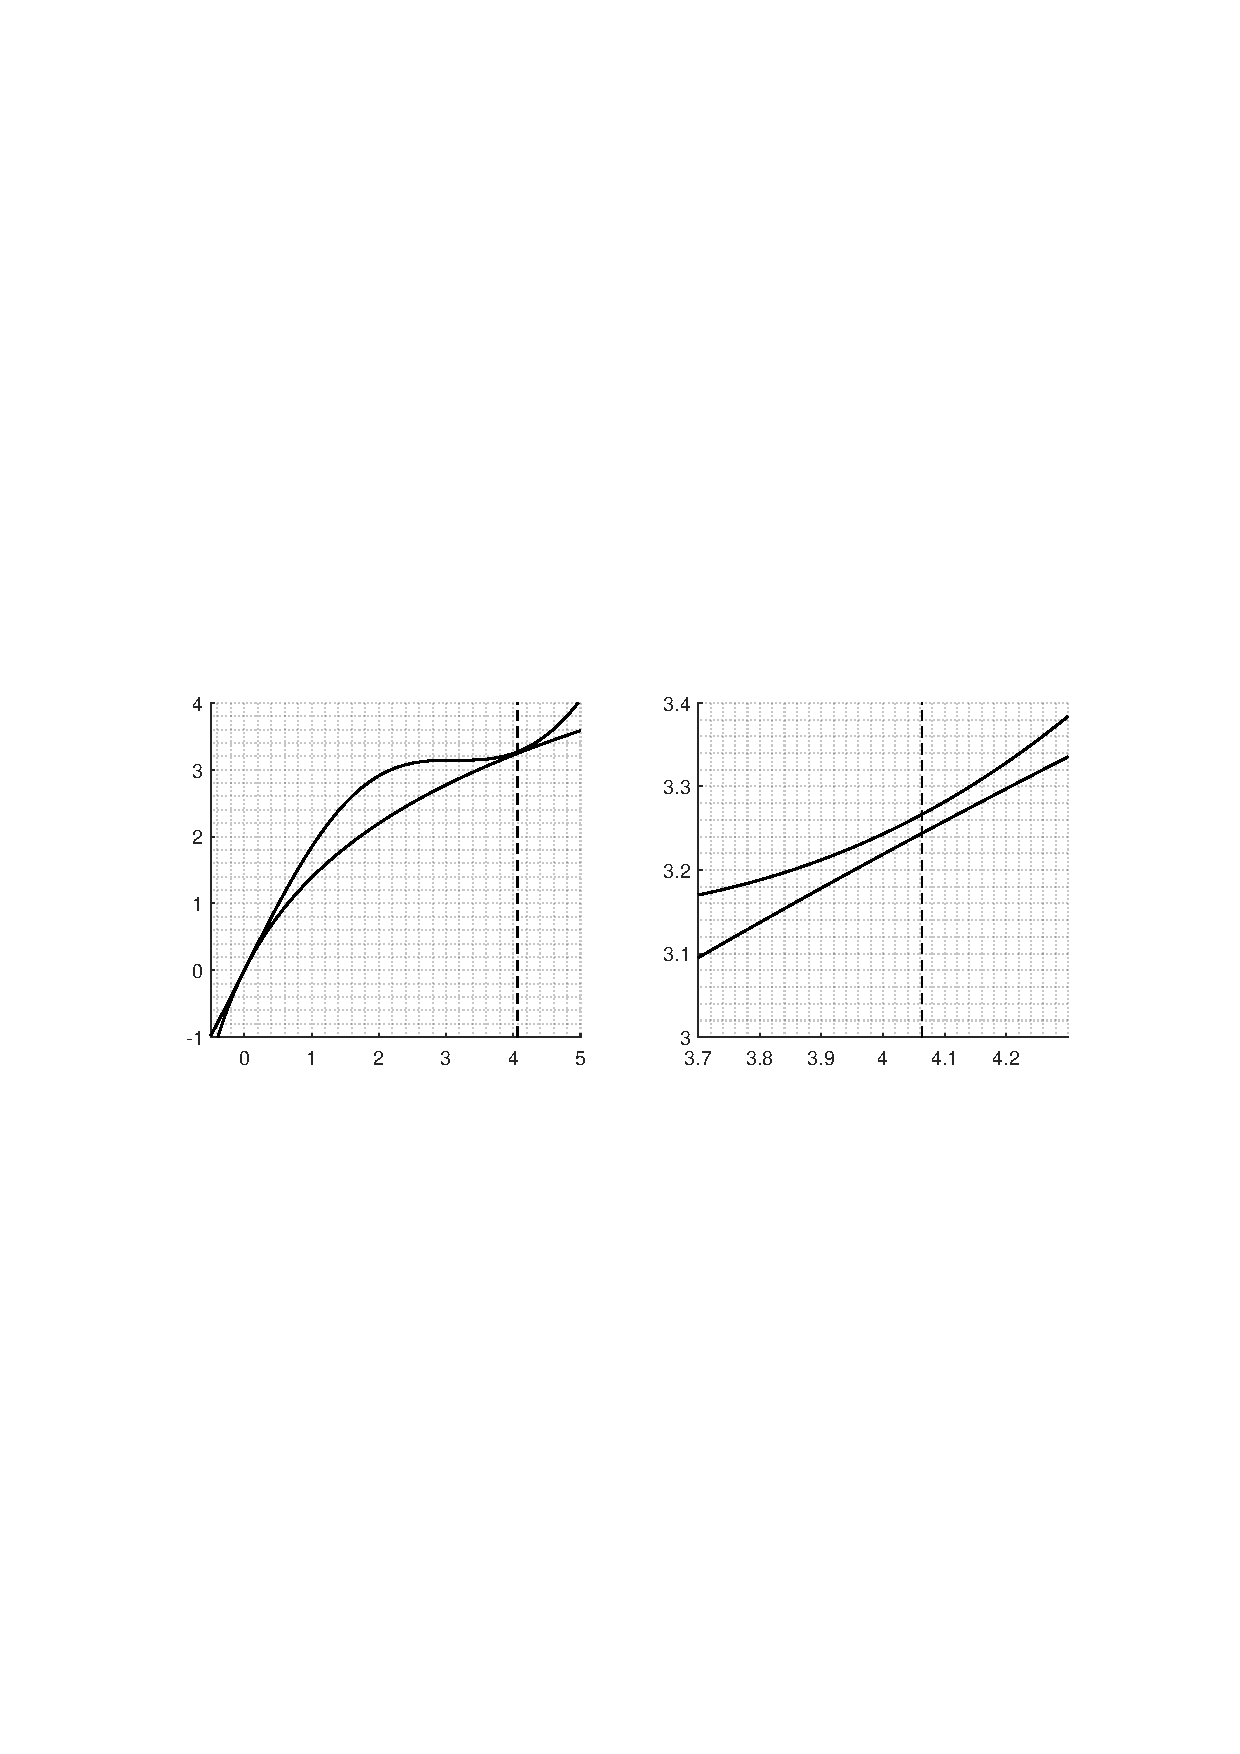
\includegraphics[width=0.95\linewidth]{x+sin(x)大于2ln(x+1)}
\end{figure} 

若$ x>0 $,则
\begin{gather*}
    \int_{0}^{x}(t+\sin t)\d t>\int_{0}^{x}2\ln(t+1)\d t \\
    \dfrac{1}{2}x^2+1-\cos x > 2(x+1)\ln(x+1) -2x
\end{gather*}
这样就又得到了一个新的不等式。

\item (2020,高考全国III卷)定义函数$ f(x)=x^3-\dfrac{3}{4}x+c $,
若$ f(x)=0 $有一个绝对值不大于1的实根,求证:所有实根的绝对值都不大于1.\\
\textbf{方法一}\ $ f'(x)=3x^2-\dfrac{3}{4}=3(x-\dfrac{1}{2})(x+\dfrac{1}{2}) $,因而,
$ (\dfrac{1}{2},-\dfrac{1}{4}+c) $和$ (-\dfrac{1}{2},\dfrac{1}{4}+c) $是$ f(x) $的两个极值点,
当$ c=\pm \dfrac{1}{4} $时,恰好有一个极值点落在$ x $轴上,此时极值点成为二重实根,
即$ f(x)=\left(x-\dfrac{1}{2} \right)^2(x+1)  $或$ f(x)=\left(x+\dfrac{1}{2} \right)^2(x-1)  $,
另外一个零点为$ -1 $或1.\ 结合图像进行分析,在二重实根的基础上进行上下平移,
平移后如果变成一个实根和两个复根,实根的绝对值必然大于1,不符合题目要求,
所以$ -\dfrac{1}{4}\leq c \leq \dfrac{1}{4} $,% 此时的三个实根绝对值明显都小于1.
设$ u $是$ f(x) $的一个实根,那么$ -\dfrac{1}{4}\leq c=-u^3+\dfrac{3}{4}u \leq \dfrac{1}{4} $, 
$ \begin{cases}
    u^3-\dfrac{3}{4}u-\dfrac{1}{4}=(u-1)(u+\dfrac{1}{2})^2 \leq 0 \\
    u^3-\dfrac{3}{4}u+\dfrac{1}{4}=(u+1)(u-\dfrac{1}{2})^2 \geq 0 
\end{cases} $,$ -1 \leq u \leq 1 $,即实根的绝对值不大于1.\\
\\
\textbf{方法二}$ ^* $使用韦达定理:$ x_1+x_2+x_3=0,x_1x_2+x_1x_3+x_2x_3=-\dfrac{3}{4} $,
\begin{align*}
    &  x_2x_3=-\dfrac{3}{4}-x_1(x_2+x_3)=-\dfrac{3}{4}-x_1(-x_1)=x_1^2-\dfrac{3}{4}  \\
    & x_1^2+x_2^2+x_3^2=(x_1+x_2+x_3)^2-2(x_1x_2+x_1x_3+x_2x_3) =\dfrac{3}{2}  \\
    & (x_2^2-1)+(x_3^2-1)=-x_1^2-\dfrac{1}{2} < 0\ (\text{说明两个括号内不能都为正})
\end{align*}
\vspace{-0.7cm}
\begin{align*}
    (x_2^2-1)(x_3^2-1)=(x_2x_3)^2-(x_2^2+x_3^2)+1 = &
    \left( x_1^2-\dfrac{3}{4} \right)^2-\left( \dfrac{3}{2}-x_1^2\right)  +1\\
    = & \left( x_1^2-\dfrac{1}{4}\right) ^2 \geq 0
\end{align*}
说明$ x_2^2\leq 1,x_3^2\leq 1 $. 读者可能会注意到,证明过程中并没有使用$ x_1^2\leq 1 $这个条件,
其实,在假设方程存在三个实根的时候,就已经隐含了这个条件。因为,如果方程的根是一个实根和两个复根,
那就不存在绝对值不大于1的实根了。\\
\textbf{方法三}\ 使用三倍角公式,因为这个三次方程恰好缺少二次项。
假设$ x_1=\cos \theta \in [-1,1] $是方程的一个实根,那么$ f(x_1)
=f(\cos \theta)=\dfrac{1}{4}(4\cos^3 \theta-3\cos \theta)+c=\dfrac{1}{4}\cos3\theta + c=0 $,
因为$ \cos3\theta=\cos3(\theta+\dfrac{2\pi}{3})=\cos3(\theta+\dfrac{4\pi}{3}) $,
所以$ x_2=\cos(\theta+\dfrac{2\pi}{3}),x_3=\cos(\theta+\dfrac{4\pi}{3}) $也是方程的根,
这两个根的绝对值显然小于等于1.  \\
\textbf{注}:此题的背景是:$ n $次首一多项式在区间$ [-1,1] $上的最大值不小于$ \dfrac{1}{2^{n-1}} $.

\item 设$ 1<x_1<x_2 $,且$ x_1^{x_2}=x_2^{x_1} $,求证:$ x_1 x_2>\e^2 $. \\
\textbf{解}\ 等价于证明$\ln x_1+\ln x_2>2 $。在$ x_1^{x_2}=x_2^{x_1} $两边同时
取自然对数,有$ x_2\ln x_1=x_1\ln x_2 $,于是
\begin{gather}
	\dfrac{\ln x_1}{x_1}=\dfrac{\ln x_2}{x_2}=\dfrac{\ln x_2
		+\ln x_1}{x_2+x_1}= \dfrac{\ln x_2-\ln x_1}{x_2-x_1} 
	\label{lnx_x极值偏移1}\\
	\ln x_1+\ln x_2=\dfrac{x_2+x_1}{x_2-x_1}(\ln x_2-\ln x_1)=\dfrac{\dfrac{x_2}{x_1}+1}{\dfrac{x_2}{x_1}-1}
	\ln \dfrac{x_2}{x_1} \label{lnx_x极值偏移2}
\end{gather} 
令$ t=\dfrac{x_2}{x_1}>1 $,则要证明$ \dfrac{t+1}{t-1}\ln t>2 $,如果直接将
$ \dfrac{t+1}{t-1}\ln t $对$ t $求导,则计算量太大,应当尽量避免使用两个函数乘或除的
求导法则。设$ g(t)=\dfrac{2(t-1)}{t+1}-\ln t $.则
$ g'(t)=-\dfrac{(t-1)^2}{t(t+1)^2}<0 $.所以,$ g(t)<g(1)=0 $,即
\begin{align}\label{2(t-1)/(t+1)<lnt}
	\dfrac{2(t-1)}{t+1}<\ln t \quad (t>1)
\end{align}
于是,$\ln x_1+\ln x_2=\dfrac{x_2+x_1}{x_2-x_1}(\ln x_2-\ln x_1)>2 $,同时有
\begin{gather}\label{对数均值不等式右半部分}
	\dfrac{x_2-x_1}{\ln x_2-\ln x_1}<\dfrac{x_1+x_2}{2}
\end{gather}

(\ref{2(t-1)/(t+1)<lnt})式与
(\ref{lnt帕德逼近})式是密切相关的。如果$ 0<t<1 $,那么
\begin{align}\label{2(t-1)/(t+1)>lnt}
	\dfrac{2(t-1)}{t+1}>\ln t \quad (0<t<1)
\end{align}
\textbf{推广1}\ 因为$ \dfrac{\ln x}{x} $在$ x=\e $处取得极大值$ \dfrac{1}{\e} $,所以$ 1<x_1<\e<x_2 $. 令$ \ln x_1=X_1\in (0,1),\ \ln x_2=X_2\in(1,+\infty) $,那么$ x_1=\e^{X_1},\ x_2=\e^{X_2},\ \dfrac{X_1}{\e^{X_1}}=\dfrac{X_2}{\e^{X_2}},\ X_1+X_2>2 $,
这就是2010年天津高考题。进一步地,设$ \ln\dfrac{\e^{X_1}}{X_1}=X_1-\ln X_1=\ln\dfrac{\e^{X_2}}{X_2}=X_2-\ln X_2=m>1 $\footnote{\ $ y=xe^x $的反函数为$ x=ye^y $,它被称为Lambert W函数。
如果将$ ye^y $取自然对数,并令其等于$ x $,即$ x=y+\ln y $,
这个新的函数被称为Wright Omega函数,暂且将其记为$ y=WO(x) $. $ X-\ln X=m $,令$ X=-u $,则$ -u-\ln(-u)=-u-\ln(-1)-\ln u=m,\ u+\ln u=-m-\ln(-1),\ u=WO(-m-\ln(-1)),\ X=-u=-WO(-m-\ln(-1)) $,根据欧拉公式,$ \e^{\i(\pi+2k\pi)}=\cos(\pi+2k\pi)+\i\sin(\pi+2k\pi)=-1 $,所以$ \ln(-1)=\i(\pi+2k\pi),\ X_1=-WO(-m+\i\pi),\ X_2=-WO(-m-\i\pi) $.},那么有\footnote{(\ref{x-lnx偏移推广1})$ \sim $(\ref{x-lnx偏移推广5})式来自于知乎用户“柯西永远爱你”,https://www.zhihu.com/question/504175361/answer/2304245404 }
\begin{align}
	X_1+X_2>&\ m+\dfrac{1}{m}+\ln m>m+1>2 \label{x-lnx偏移推广1}\\
	X_1+X_2>&\ \dfrac{2}{3}(m+2\sqrt{m})>2 \label{x-lnx偏移推广2} \\
	X_1+X_2>&\ m+2-\sqrt{X_1X_2}>m+1>2\label{x-lnx偏移推广3} \\
	X_1+X_2>&\ m(1-X_1X_2)+2>2\label{x-lnx偏移推广4} \\
	X_1+X_2>&\ 4-2X_1X_2>4-\dfrac{6}{2m+1}>4-\dfrac{4}{m+1}>2
		\label{x-lnx偏移推广5} 
\end{align} 
下面对以上不等式作一些粗略分析。
\begin{align} 
	&\left.
	\begin{aligned} \label{对X_1的范围估计}
		& m=X_1-\ln X_1<1-\ln X_1 \\
		& m=X_1-\ln X_1>-\ln X_1	
	\end{aligned} \right\} \Rightarrow \ \e^{-m}<X_1<\e^{1-m} \\
	&\left.
	\begin{aligned} \label{对X_2的范围估计}
		& m=X_2-\ln X_2> X_2-\sqrt{X_2} \\
		& m=X_2-\ln X_2< X_2
	\end{aligned} \right\} \Rightarrow \ m<X_2<\left(\dfrac{1+
	\sqrt{1+4m}}{2}\right)^2 
\end{align}
因为$ X_1X_2<\e^{1-m}\cdot \left(\dfrac{1+\sqrt{1+4m}}{2}\right)^2 $,随着$ m\to \infty $,显然有$ X_1X_2 \to 0 $. 

根据不等式(\ref{2(t-1)/(t+1)<lnt})和(\ref{2(t-1)/(t+1)>lnt}),
\begin{gather}
 m=X_1-\ln X_1>X_1-\dfrac{2(X_1-1)}{X_1+1}=\dfrac{X_1^2-X_1+2}{X_1+1} 
\label{Pade逼近对X_1的范围估计} \\
 m=X_2-\ln X_2<X_2-\dfrac{2(X_2-1)}{X_2+1}=\dfrac{X_2^2-X_2+2}{X_2+1} 
\label{Pade逼近对X_2的范围估计}	\\	
	 -m(X_1+1)<\ -X_1^2+X_1-2 \nonumber \\
	  m(X_2+1)<\ X_2^2-X_2+2 \nonumber
\end{gather}
以上两式相加可得:
\begin{gather*}
	m(X_2-X_1)<(X_2-X_1)(X_2+X_1-1)  \\
	m<X_2+X_1-1 \\
    X_1+X_2>m+1
\end{gather*}
前面也提到过,用$ \dfrac{X^2-X+2}{X+1} $作为$ X-\ln X $的近似替代,精度不如$ X-\ln X $的$ (2,1) $阶帕德逼近 $ \dfrac{3X^2-2X+5}{4X+2} $. \\
\textbf{推广2}\ 如果$ \alpha>0, 1<x_1<x_2 $,且$ \dfrac{\ln x_1}{x_1^{\alpha}}=
\dfrac{\ln x_2}{x_2^{\alpha}} $,那么有$ x_1 x_2>\e^{2/\alpha},\ \ln x_1+\ln x_2>\dfrac{2}{\alpha} $. 

% shuiqiu.m
\item $ ^* $ (微信公众号:水球命题组)函数
$ f(x)=\e^x-x-a \ (a\in \textbf{R}) $有两个零点$ x_1,x_2 \ (x_1<x_2) $.\\
(I)求$ a $的取值范围;\\
(II)求证:$ 1-a<x_1+x_2<\dfrac{2}{3}(1-a) $; \\
(III)求证:$ x_1^2+x_2^2<(a+3)(a-1) $. \\
\textbf{解}\ (I) $ f'(x)=\e^x-1 $,$ f(x) $在$ (-\infty,0) $上单调递减,在$ (0,+\infty) $上单调递增,在$ x=0 $处取得极小值1,所以$ a>1 $. \\
(II)和(III)的难度较大,过程也十分繁琐,这里只做一些粗略分析,完整过程可查阅脚注中的链接\footnote{
    一道网红导数题的命制背景与解法探究 https://zhuanlan.zhihu.com/p/453748970 \\
    一道秒杀MST团队的导数题解析 https://mp.weixin.qq.com/s/PvzUhhAVZx2duAO-Qor2qw \\
    水神导数闯关练第九题解析 https://zhuanlan.zhihu.com/p/383370671 }。

如果做代换$ \e^x=X $,那么$ \e^x-x=a $可化为$ X-\ln X=a $,而$ x_1+x_2=\ln X_1+\ln X_2=\ln(X_1X_2) $,问题就转化为求$ X_1X_2 $的范围,上一题的推广1中已做过分析,(把$ m $换成$ a $)
\begin{gather*}
    \e^{-a}<X_1<\e^{1-a},\q -a<\ln X_1<1-a \\
    a<X_2<\left(\dfrac{1+\sqrt{1+4a}}{2}\right)^2,\q \ln a<\ln X_2<
    \ln\left(a+\dfrac{1}{2}\sqrt{4a+1}+\dfrac{1}{2}\right) \\
    a \e^{-a}<X_1X_2<\e^{1-a}\cdot \left(\dfrac{1+\sqrt{1+4a}}{2}\right)^2=
    \e^{1-a}\cdot \left(a+\dfrac{1}{2}\sqrt{4a+1}+\dfrac{1}{2}\right) \\
    \ln a -a <\ln(X_1X_2)<1-a+\ln\left(a+\dfrac{1}{2}\sqrt{4a+1}+\dfrac{1}{2}\right)
\end{gather*}
当$ a $足够大时,必有
\begin{gather*}
    1-a<\ln a -a <x_1+x_2=\ln(X_1X_2)<1-a+\ln\left(a+\dfrac{1}{2}
    \sqrt{4a+1}+\dfrac{1}{2}\right)<\dfrac{2}{3}(1-a)
\end{gather*} 
所以(II)中的不等式(在$ a $足够大时)成立。

当然也可以直接得到$ x_1,x_2\ (x_1<0<x_2) $的范围估计,而不借助前面已经得出的$ X_1,X_2 $的范围,过程如下:
\begin{align*}
    \begin{aligned}
        & -x_1<a=\e^{x_1}-x_1<1-x_1 \ \Rightarrow \ -a<x_1<-a+1 \\
        & \e^{x_2}-\e^{x_2/2}<a=\e^{x_2}-x_2<\e^{x_2} \ \Rightarrow \ 
        \ln a<x_2<\ln\left(a+\dfrac{1}{2}\sqrt{4a+1}+\dfrac{1}{2}\right)
    \end{aligned} 
\end{align*}
上面使用了不等式$ \e^{x/2}>x\ (x\in \textbf{R}) $.

$ \e^x-x $在$ x=0 $处的$ (2,2) $阶帕德逼近为$ R_{2,2}(x)=
\dfrac{36-12x+19x^2}{36-12x+x^2}=\dfrac{36-12x+19x^2}{(x-6)^2} $,
这一逼近属于交叉型,图像如下,
\begin{figure}[!ht]
    \centering
    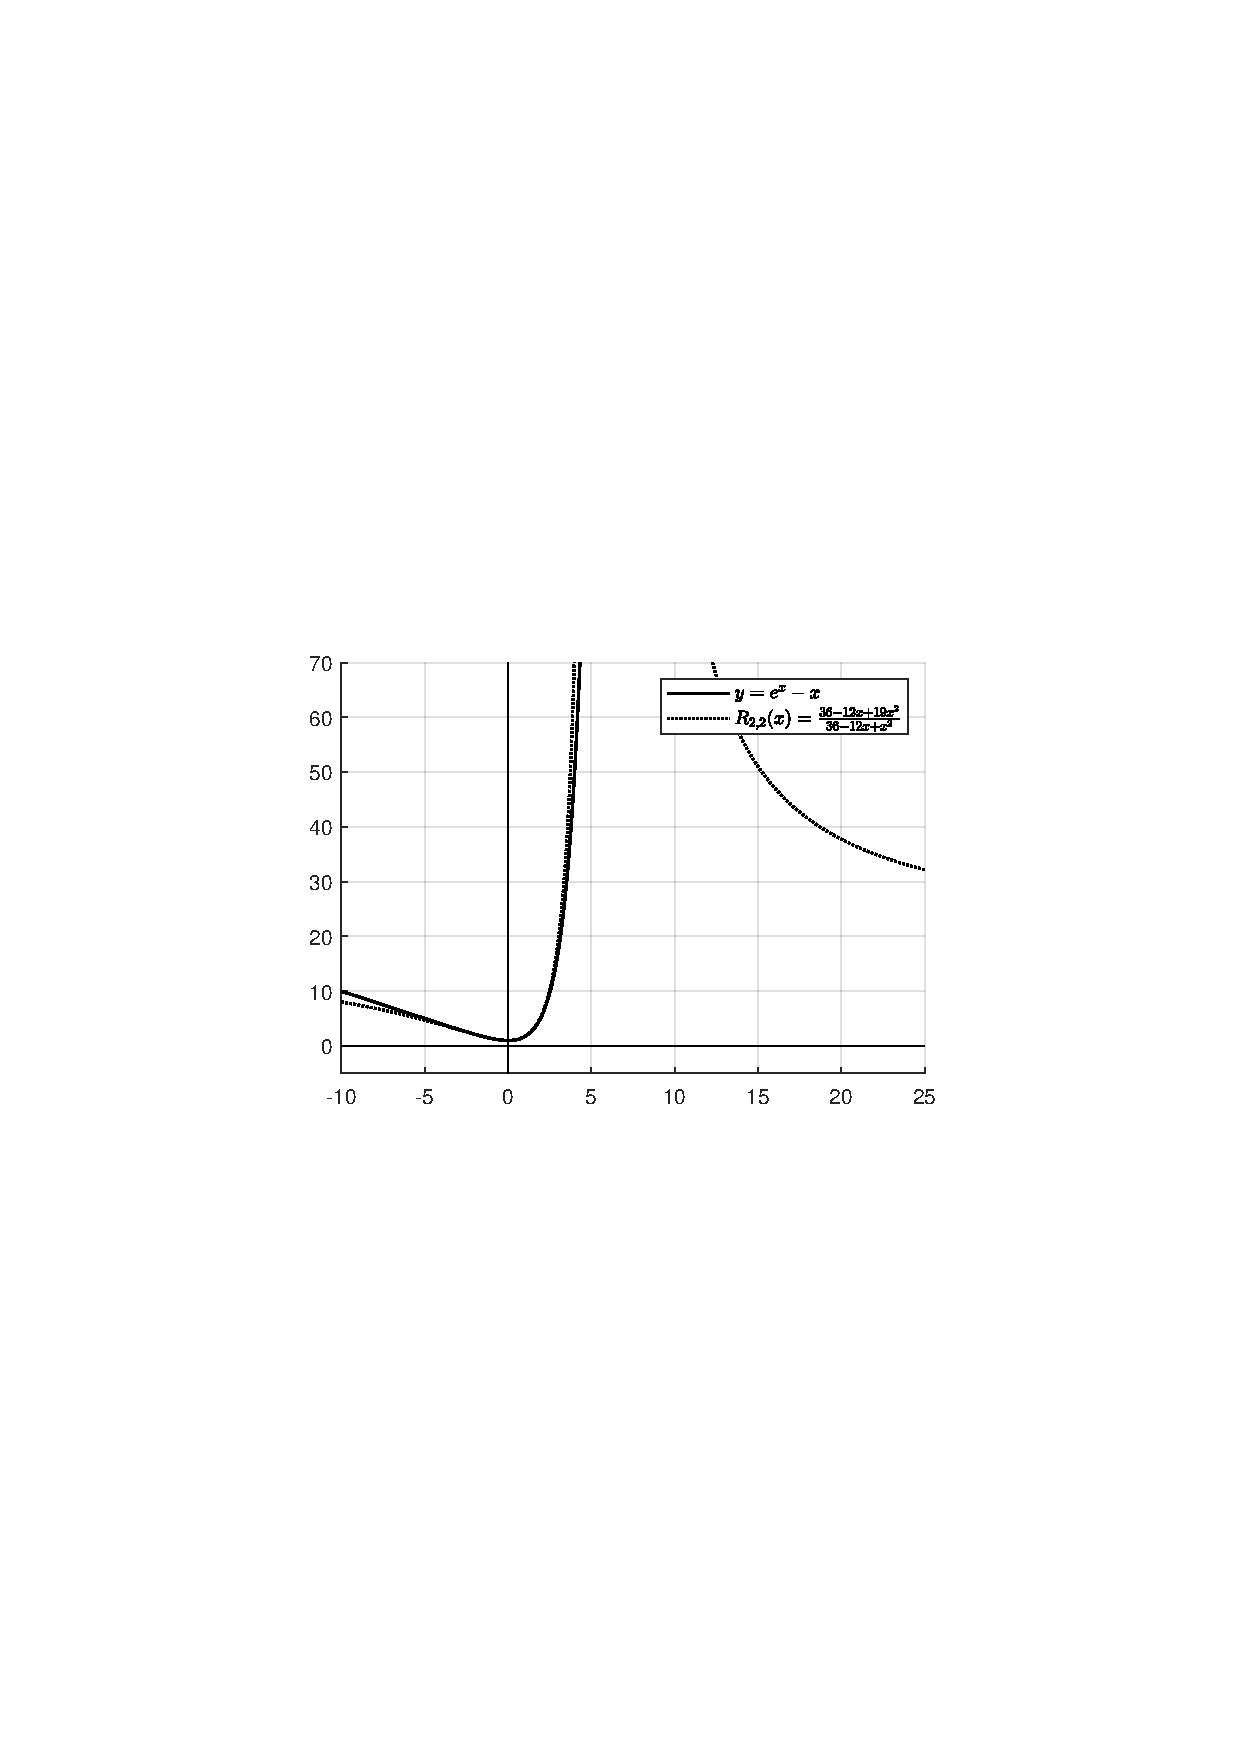
\includegraphics[width=0.6\linewidth]{水球ex-x-a}
\end{figure}
当$ x<0 $时,$ R_{2,2}(x)<\e^x-x $,
当$ 0<x<6 $时,$ R_{2,2}(x)>\e^x-x $. 
设$ R_{2,2}(x)=a $的两个解为$ u_1,u_2 $,则
\begin{gather*}
    (19-a)x^2-12(1-a)x+36(1-a)=0 \\
    u_1+u_2=\dfrac{12(1-a)}{19-a}
\end{gather*}
显然有$ x_1+x_2>u_1+u_2 $,再假设$ u_1+u_2>1-a $,解得$ 1<a<7 $.
前面已经提过,当$ a $足够大时,$ 1-a<\ln a-a<x_1+x_2 $,
对于这一不等式,$ a>\e $就算“足够大”。

总结一下,对$ x_1+x_2>1-a $的证明分了两种情况,\\
\mycircled{1} 当$ 1<a\leq \e\ (<7) $时,由
\begin{gather*}
    x_1+x_2>u_1+u_2=\dfrac{12(1-a)}{19-a}>1-a
\end{gather*}
可知结论成立。\\
\mycircled{2} 当$ a> \e $时,由$ x_1+x_2>\ln a-a>1-a $
可知结论成立。

$ \e^x-x $在$ x=0 $处的$ (1,2) $和$ (2,1) $阶帕德逼近分别为
$ R_{1,2}(x)=\dfrac{2x-6}{3x^2+2x-6} $和
$ R_{2,1}(x)=\dfrac{-3x^2+2x-6}{2x-6} $,图像如下:
\begin{figure}[H]
    \centering
    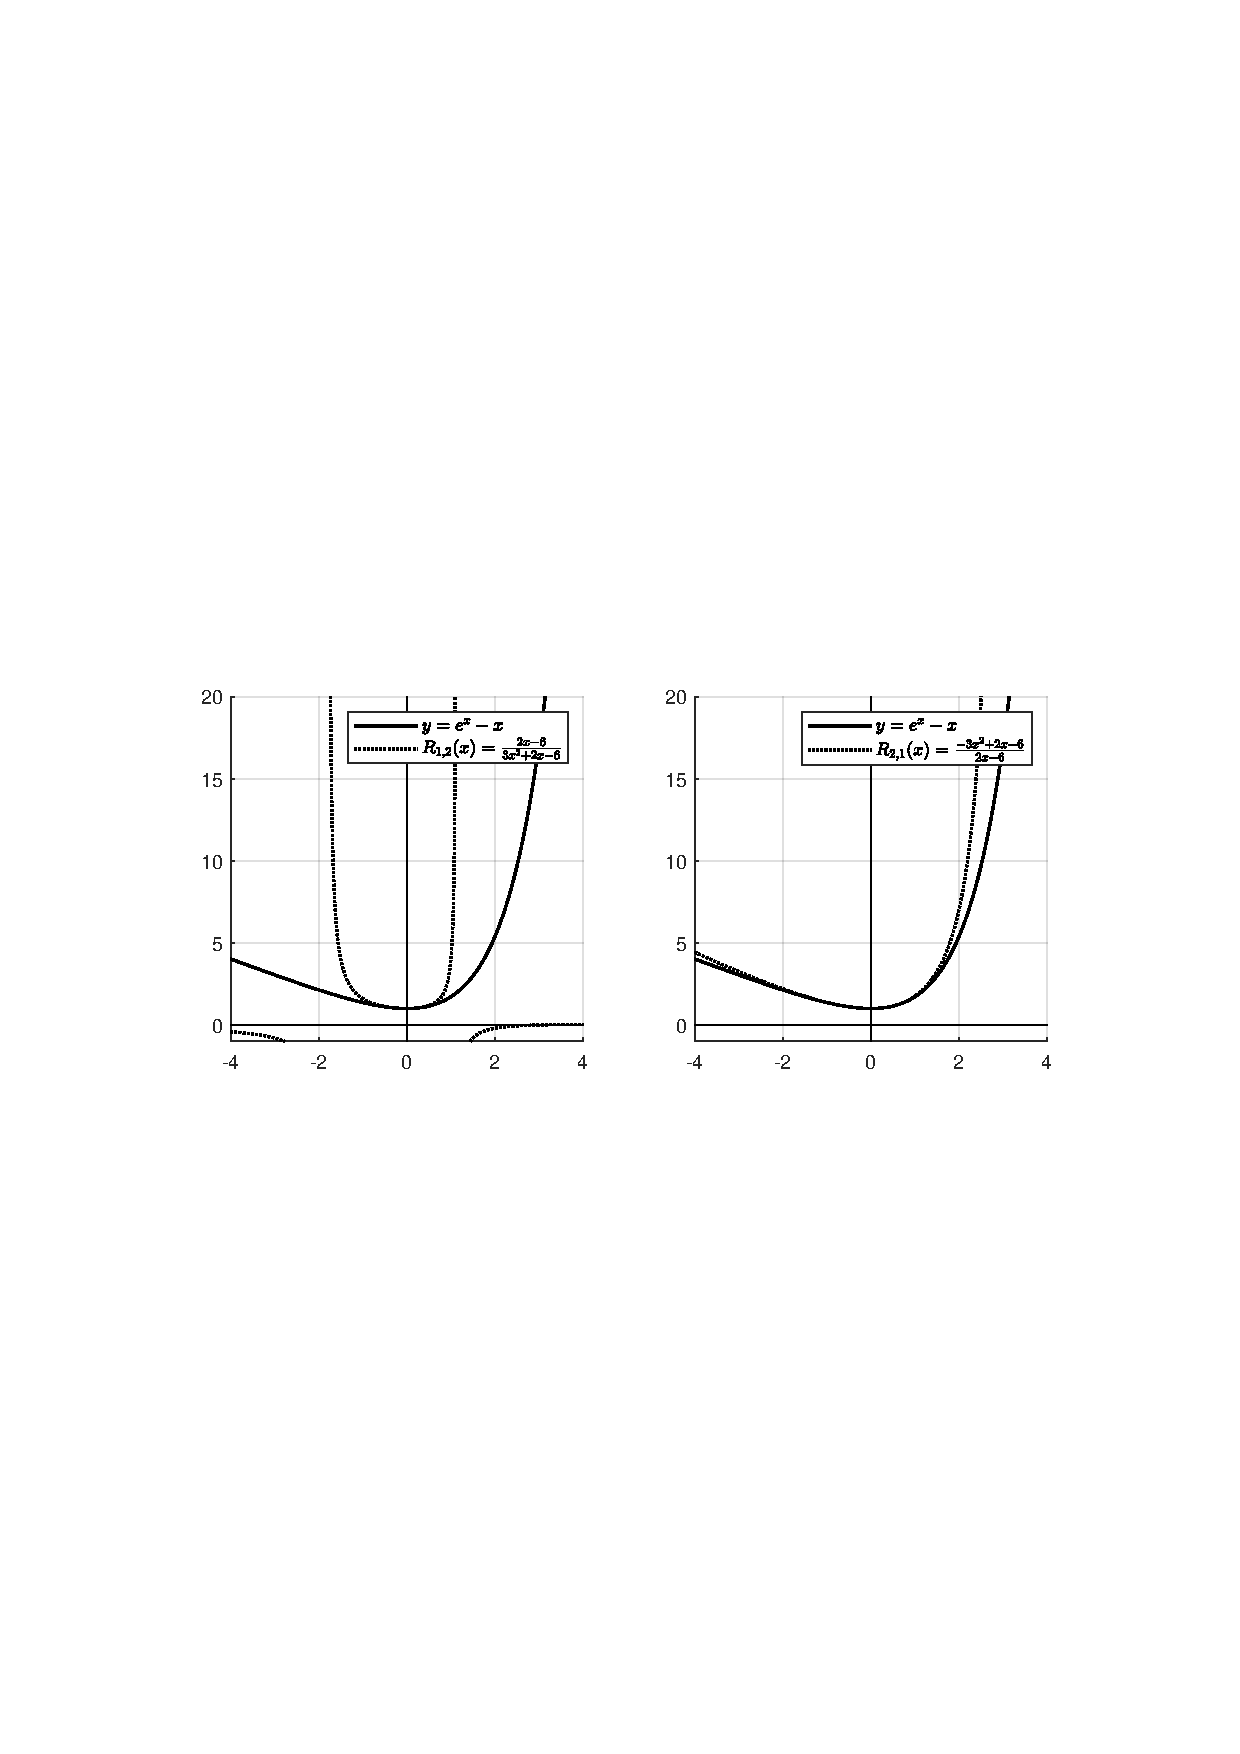
\includegraphics[width=0.9\linewidth]{水球ex-x-a不交叉型}
\end{figure}
两者都属于不交叉型,
对于本题没有用处,对于证明$ |x_2-x_1|>\varphi(a) $型的不等式可能有用。

再考虑第(III)问,
\begin{gather*}
    (a-1)^2<x_1^2=(\ln X_1)^2<a^2 \\
    (\ln a)^2<x_2^2=(\ln X_2)^2<
    \left[\ln\left(a+\dfrac{1}{2}\sqrt{4a+1}+\dfrac{1}{2}\right)\right]^2
\end{gather*}
当$ a $足够大时,必有
\begin{gather*}
    x_1^2+x_2^2=(\ln X_1)^2+(\ln X_2)^2<a^2+\left[\ln\left(a+\dfrac{1}{2}
    \sqrt{4a+1}+\dfrac{1}{2}\right)\right]^2<a^2+2a-3
\end{gather*} 
所以(III)中的不等式(在$ a $足够大时)成立。

还可以证明:当$ x<0 $时,$ \e^x-x<\sqrt{x^2+1} $,所以:
\begin{gather*}
    a=\e^{x_1}-x_1<\sqrt{x_1^2+1},\ a^2-1<x_1^2
\end{gather*}

(\ref{对X_2的范围估计})式对$ X_2 $的范围做出的估计,使用了不等式$ \sqrt{X}>\ln X \ (X>0) $. 如果要提高当$ a $很大时的估计精度,可改用$ \sqrt{X}-0.6 >\ln X \ (X>0) $\footnote{\ 函数$ y=\sqrt{x}-\ln x $在$ x=4 $处取得极小值$ 2(1-\ln2)\approx 0.613705\cdots $},那么
\begin{gather*}
    X_2-\sqrt{X_2}+0.6<X_2-\ln X_2=a \\
    X_2< \left(\dfrac{1+\sqrt{-1.4+4a}}{2}\right)^2
\end{gather*}
如果要进一步提高当$ a $很大时的估计精度,可改用不等式$ \sqrt[3]{X}+0.3 >\ln X \ (X>0) $,再利用三次方程求根公式,此时反求出$ X_2 $的范围的表达式十分繁琐,在此略去。

如果对本题使用泰勒级数,$ \e^x $在$ x=0 $处的泰勒级数$ 1+x+\dfrac{1}{2}x^2 $
与$ \e^x $是交叉的,因为$ x_1<0<x_2 $,所以,
\begin{gather*}
    1+\dfrac{1}{2}x_2^2 < \e^{x_2}-x_2=a=\e^{x_1}-x_1<1+\dfrac{1}{2}x_1^2 \\
    x_2^2<2(a-1)<x_1^2
\end{gather*} 

可惜,是$ x_1^2>a^2-1 $,而不是$ x_1^2<a^2-1 $,否则,把$ \begin{cases}
    x_1^2<a^2-1 \\
    x_2^2<2(a-1)
\end{cases}$两式相加就能得到$ x_1^2+x_2^2<a^2+2a-3=(a+3)(a-1) $.

(II)和(III)问的困难之处在于,方程$ \e^x-x=a $(或$ X-\ln X=a $)
的解无法用$ a $显式表示,而上面介绍的解决方法可以用一句话概括:
用可以显式反解的函数近似代替题目中的函数。比如$ X-\sqrt{X}=a $,
$ X-(\sqrt[3]{X}+0.3)=a $, $\dfrac{X^2-X+2}{X+1}=a $,
$ R_{2,2}(x)=\dfrac{36-12x+19x^2}{36-12x+x^2}=a $,都能显式反解,
即用$ a $显式表示$ X $或$ x $. 除了基本初等函数可以显式反解外,
几乎只剩下次数较低的多项式函数(泰勒级数)和分式函数(帕德逼近)。
三次和四次方程的求根公式过于复杂,在高考中几乎无法使用,
所以多项式主要考虑使用一次和二次的。不过,泰勒级数和帕德逼近
都只在展开点附近有比较好的精度。有能力的读者,还可以使用拉格朗日反演,以及隐函数求导法。

\item (2020,浙江高考)已知$ 1<a\leq 2 $,函数$ f(x)=\e^x-x-a $.\\
(I)证明:$ f(x) $在$ (0,+\infty) $上有唯一零点; \\
(II)记$ x_0 $为$ f(x) $在$ (0,+\infty) $上的零点,证明:

(i) $ \sqrt{a-1}< x_0 < \sqrt{2(a-1)} $;

(ii) $ x_0f(\e^{x_0})> (\e-1)(a-1)a $. \\
\textbf{解}\ 以下过程将要多次用到$ \ln 2=0.6931\cdots $,
这个数值在很多题目中都用得上,请牢牢记住\footnote{人教版2019版高中数学必修第一册,第四章“指数函数与对数函数”(125页)要求用计算器算出$ \ln 2,\ln 3 $的数值,因此高考试卷上即使没有提供这些数值,直接使用也是可以的。}。\\
(I) $ f'(x)=\e^x-1>0\ (x>0) $,$ f(x) $在$ (0,+\infty) $上单调递增,
$ f(0)=1-a<0,\ f(2\ln 2)=4-2\ln 2-a>0 $,由零点存在定理,
$ f(x) $在$ (0,+\infty) $上有唯一零点,且零点位于区间$ (0,2\ln2) $内。\\
(II) (i) $ \e^{x_0}-x_0=a $,逆向分析待证不等式,$ x_0^2<2(a-1)=2(\e^{x_0}
-x_0-1),\ 1+x_0+\dfrac{1}{2}x_0^2< \e^{x_0}\ (0<x_0<2\ln 2) $,由$ \e^x $在$ x=0 $
处的泰勒展开,或者直接求导,都很容易验证该不等式。下面证明另一半不等式$ \sqrt{a-1}< x_0 $。\\
\textbf{方法一}\ \ $ a-1=\e^{x_0}-x_0-1< x_0^2 $,
只需证$ \e^{x_0}< 1+x_0+x_0^2\ (0<x_0<2\ln 2) $. 令
$ g(x)=\e^x-1-x-x^2\ (0<x<2\ln 2) $,则$ g'(x)=\e^x-1-2x,\ g'(0)=0,\ g''(x)=
\e^x-2,\ g''(\ln 2)=0 $,说明$ g'(x) $在$ (0,\ln 2) $上单调递减,在$ (\ln2,
2\ln2) $上单调递增,因为$ g'(\ln2)=1-2\ln 2<0,\ g'(2\ln 2)=3-4\ln 2>0 $,
所以$ g'(x) $在$ (\ln2,2\ln2 ) $内有且仅有一个零点,记为$ z_0 $. 于是,$ g(x) $在
$ (0,z_0) $上单调递减,在$ (z_0,2\ln 2) $上单调递增,在$ x=z_0 $处取得极小值,
而$ g(0)=0,\ g(2\ln 2)=3-2\ln2-(2\ln2)^2\approx -0.3077<0 $,所以,
$ g(x)<0 $在$ (0,2\ln2) $上恒成立,$ \sqrt{a-1} < x_0 $得证。\\
\textbf{方法二}\ 令$ \psi(x)=\dfrac{x^2+x+1}{\e^x}\ (0<x<2\ln 2) $,则$ \psi'(x)=\dfrac{x(1-x)}{\e^x} $,$ \psi(x) $在$ (0,1) $上单调递增,在$ (1,2\ln2) $上单调递减,$ \psi(0)=1,\ \psi(2\ln 2)=\dfrac{(2\ln 2)^2+2\ln 2+1}{4}>1 $,所以,$ \psi(x)>1 $在$ (0,2\ln2) $上恒成立。\\
\textbf{方法三}\ 利用(\ref{e^x<(2+x)/(2-x)})式(考试时需要证明),
$ \e^{x}<\dfrac{2+x}{2-x},\ x\in (0,2) $,那么
\begin{gather*}
    f(\sqrt{a-1})=\e^{\sqrt{a-1}}-\sqrt{a-1}-a<\dfrac{2+\sqrt{a-1}}{2-\sqrt{a-1}}
    -\sqrt{a-1}-a=\\ \dfrac{1-a-\sqrt{a-1}+a\sqrt{a-1}}{2-\sqrt{a-1}}=
    \dfrac{(a-1)(\sqrt{a-1}-1)}{2-\sqrt{a-1}}\leq 0
\end{gather*}
所以,$ f(x) $在区间$ (\sqrt{a-1},2\ln2) $上存在唯一实根$ x_0 $,显然$ x_0>\sqrt{a-1} $.\\
(ii)题目中出现了$ f(\e^{x_0}) $,如果不做任何转换,那么$ f(\e^{x_0})=\e^{\e^{x_0}}-
\e^{x_0}-a $,出现了指数函数和指数函数的复合,无法继续计算了。显然应该把$ \e^{x_0} $换成$ x_0+a $. 
%\textbf{方法一}
\begin{gather*}
    x_0f(\e^{x_0})=x_0f(x_0+a)=x_0(\e^{x_0+a}-x_0-2a)=x_0[(x_0+a)\e^a-x_0-2a]\\
    =(\e^a-1)x_0^2+a(\e^a-2)x_0 >(\e^a-1)x_0^2>a(\e-1)x_0^2>a(\e-1)(a-1)
\end{gather*}
其中应用了$ \e^x\geq \e x $\ (等号仅在$ x=1 $处成立),$ \e^a-1>\e a-1>\e a-a=a(\e-1) $. \\
%\textbf{方法二}\ \ 
%$ x_0f(\e^{x_0})=x_0f(x_0+a)=x_0(\e^{x_0+a}-x_0-2a)=x_0\e^{x_0+a}-x_0^2-2ax_0 $,令$ h(x)=x\e^{x+a}-x^2-2ax\ (x>0) $,则$ h'(x)=(x+1)\e^{x+a}-2x-2a,\ h''(x)=(x+2)\e^{x+a}-2>0\ (x>0) $,说明$ h'(x) $在$ (0,+\infty) $上单调递增,$ h'(x)>h'(0)=\e^a-2a>0 $(容易证明,$ \e^x\geq \e x >2x $在$ (0,+\infty) $上恒成立),所以,$ h(x) $在$ (0,+\infty) $上单调递增,$ h(x_0)>h(\sqrt{a-1})=\sqrt{a-1}(\e^{\sqrt{a-1}+a}-\sqrt{a-1}-2a) $,如果能证明$ h(\sqrt{a-1})>(\e-1)(a-1)a $,那就解决了本题,采用逆向分析法,
%\begin{gather*}
%    \sqrt{a-1}(\e^{\sqrt{a-1}+a}-\sqrt{a-1}-2a)>(\e-1)(a-1)a \\
%    \e^{\sqrt{a-1}+a}-\sqrt{a-1}-2a>(\e-1)a\sqrt{a-1} 
%\end{gather*}
%又因为$ 1+x+\dfrac{1}{2}x^2< \e^{x}\ (x>0) $,所以只需证
%\begin{gather}
%    1+(\sqrt{a-1}+a)+\dfrac{1}{2}(\sqrt{a-1}+a)^2-\sqrt{a-1}-2a>(\e-1)a\sqrt{a-1}
%    \nonumber \\
%    a^2-a+1>2(\e-2)a\sqrt{a-1} \label{浙江2020导数1}
%\end{gather}
%证明(\ref{浙江2020导数1})式的方法1,
%\begin{gather*}
%    a^2-a+1=a^2-(\sqrt{a-1})^2>2(\e-2)a\sqrt{a-1} \\
%    \dfrac{a}{\sqrt{a-1}}-\dfrac{\sqrt{a-1}}{a}>2(\e-2)
%\end{gather*}
%令$ u=\dfrac{a}{\sqrt{a-1}}=\dfrac{a-1+1}{\sqrt{a-1}}=\sqrt{a-1}+\dfrac{1}{\sqrt{a-1}}\in [2,+\infty) $,所以$ \dfrac{a}{\sqrt{a-1}}-\dfrac{\sqrt{a-1}}{a}=u-\dfrac{1}{u}\geq 2-\dfrac{1}{2}=\dfrac{3}{2}>2(\e-2) $.
%
%证明(\ref{浙江2020导数1})式的方法2,用另一种换元法求$ \dfrac{a^2-a+1}{a\sqrt{a-1}} $的最小值,令$ t=\sqrt{a-1}\in (0,1] $,则$ a=t^2+1 $,记$ \varphi(t)=\dfrac{(t^2+1)^2-(t^2+1)+1}{t(t^2+1)}=\dfrac{t^4+t^2+1}{t(t^2+1)} $,则$ \varphi'(t)=\dfrac{t^6+2t^4-2t^2-1}{t^2(t^2+1)^2}=\dfrac{(t^2-1)(t^4+3t^2+1)}{t^2(t^2+1)^2}\leq 0 $,所以$ \varphi(t)\geq \varphi(1)=\dfrac{3}{2}>2(\e-2) $.\\
\textbf{注1}:在估计某个变量的范围的时候,越精确越好。对于本题中的$ x_0 $,其最小值
趋于0(当$ a $趋于1时),这个边界没法改进。重点在于对其最大值的估计,如果粗糙地认为
$ x_0<2 $,那么在证明$ g(x)<0 $时会遇到困难,因为$ g(x)<0 $并不是在$ (0,2) $
上恒成立,而是在$ (0,1.793282\cdots) $上恒成立,所以上面的过程使用了$ x_0 $的更精确的范围,即$ x_0<2\ln2=1.386294\cdots $,事实上,$ x_0 $的最大值为方程$ \e^x-x=2 $的正根,数值为$ 1.146193\cdots $.\\
\textbf{注2}:(II)中(i)和(ii)的原貌是$ \sqrt{a-1}\leq x_0 \leq \sqrt{2(a-1)} $和
$ x_0f(\e^{x_0})\geq (\e-1)(a-1)a $,然而,三个等号均是在$ a=1,\ x_0=0 $时才能取到,
但题目一再强调$ a>1,\ x_0>0 $,所以完全没有必要使用$ \leq,\geq $,使用$ <,> $即可。
有的人认为$ \geq $中包含了$ > $,用$ \geq $并不算错。
这当然不算错误,然而显得很别扭。按照这种“包含”的说法,
$ \geq $中也包含了$ = $,$ (a+b)^2=a^2+2ab+b^2 $
可以写成$ (a+b)^2\geq a^2+2ab+b^2 $,
难道有人认为后一种写法更合适吗?

% XinGaoKao_I_2022.m
\item \label{2022新高考I卷导数x1x2x3}(2022,新高考I卷)
已知函数$f(x)=\mathrm{e}^{x}-ax$和$g(x)=ax-\ln x$有相同的最小值。\\
(1)求$a$;\\
(2)证明:存在直线$y=b$,其与两条曲线$y=f(x)$和$y=g(x)$共有三个不同的交点,并且从左到右的三个交点的横坐标成等差数列。\\
\textbf{解}\ (1) $ f'(x)=\e^x-a $,$ g'(x)=a-\dfrac{1}{x} $,
若$ a\leq 0 $,则$ f(x),\ g(x) $均无最小值,所以$ a>0 $.
令$ f'(x)=0 $,$ x_f=\ln a $;令$ g'(x)=0 $,$ x_g=\dfrac{1}{a} $,于是
\begin{gather*}
    f(\ln a)=a-a\ln a=g\left(\dfrac{1}{a}\right)=1+\ln a
\end{gather*}
显然$ a=1 $满足上式,还需根据单调性判断是否唯一。\\ 令
$ F(a)=a-a\ln a-\ln a-1\ (a>0) $,则$ F'(a)=-\ln a-\dfrac{1}{a} $,
$ F''(a)=-\dfrac{1}{a}+\dfrac{1}{a^2} $,所以,
$ F'(a)\leq F'(1)=-1<0 $,
$ F(a) $在$ (0,+\infty) $上单调递减,$ a=1 $是唯一解。\\
(2) 当$ a=1 $时,$ f(x),g(x) $的最小值都是1,所以$ b>1 $.
而且$ y=f(x),\ y=g(x) $在区间$ (0,1) $内存在一个交点,当$ y=b $
恰好通过此交点时,其与两条曲线$y=f(x)$和$y=g(x)$共有三个不同的交点,
\begin{figure}[!ht]
    \centering
    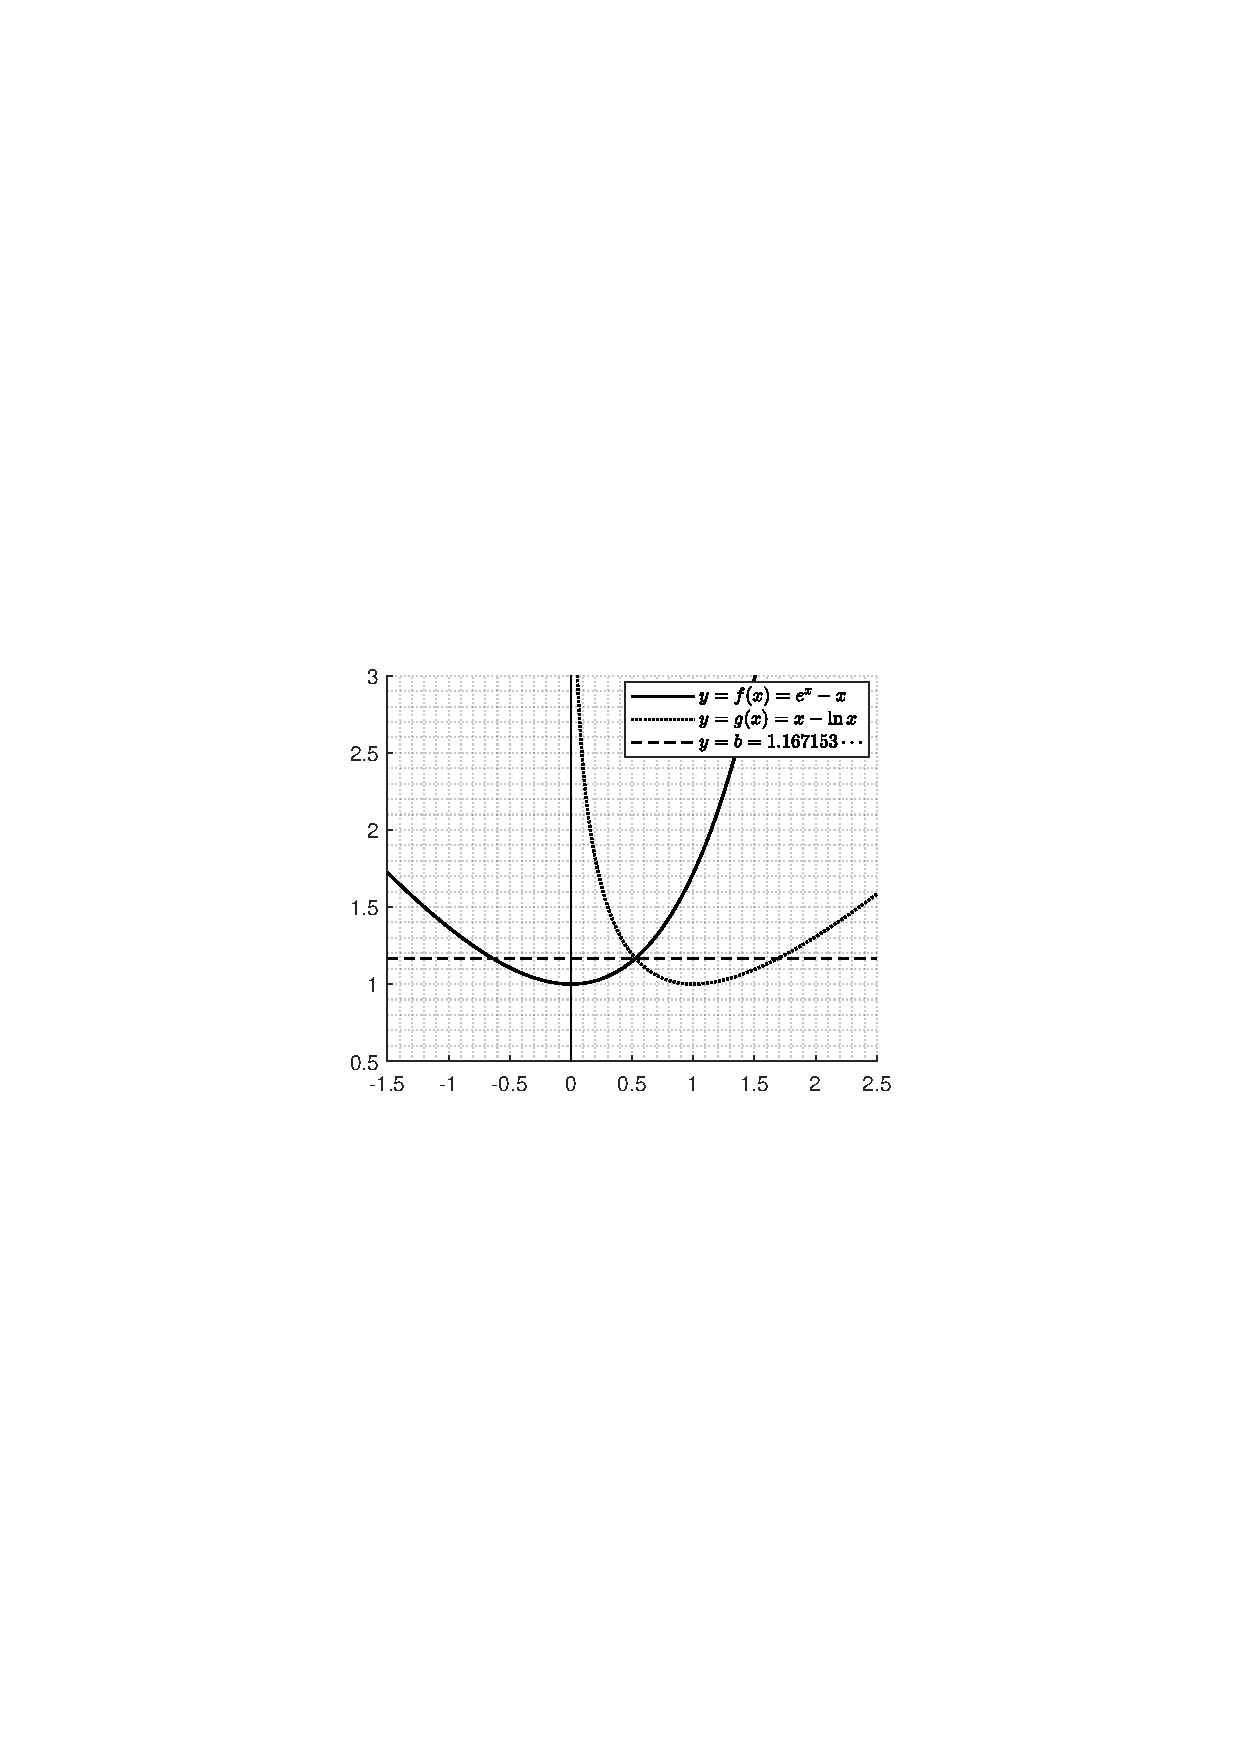
\includegraphics[width=0.5\linewidth]{2022新高考I卷}
\end{figure}
\noindent 设从左到右三个交点横坐标依次为$ x_1,x_2,x_3 $,则
\begin{gather}
    f(x_1)=f(x_2)=g(x_2)=g(x_3)=b \nonumber \\
    \e^{x_1}-x_1=\e^{x_2}-x_2=x_2-\ln x_2=x_3-\ln x_3 
    \label{2022全国x1x2x3}
\end{gather}
利用$ g(x)=f(\ln x) $\ (这是本题的关键),有
\begin{gather*}
    f(x_1)=f(x_2)=f(\ln x_2)=f(\ln x_3)=b
\end{gather*}
根据不等式$ \ln x\leq x-1<x $,方程$ x=\ln x $无解,所以
$ \begin{cases}
    x_1=\ln x_2 \\
    x_2=\ln x_3
\end{cases},\ 
\begin{cases}
    \e^{x_1}=x_2 \\
    \ln x_3=x_2
\end{cases}$. \\再结合(\ref{2022全国x1x2x3})式,
$ x_1+x_3=\e^{x_1}+\ln x_3=x_2+x_2 $,证毕。

利用软件,$ x_2=0.527447\cdots $,
$ x_1=\ln x_2=-0.639706\cdots $,$ x_3=\e^{x_2}=1.694600\cdots $. 
竟然有人发现了这三个交点横坐标成等差数列,还是令我十分吃惊的。
那么,当然要思考如何进行推广。\\ 
\textbf{推广1}\ 设$ f(x)=F(x)-x,\ g(x)=x-G(x) $,其中
$ F(x),\ G(x) $互为反函数,即$ F(G(x))=G(F(x))=x $,
$ f(x),\ g(x) $都有且仅有一个极值点,
且$ y=f(x),\ y=g(x) $至少有一个交点,
那么过其中某个交点的水平直线与$ y=f(x),\ y=g(x) $共有
三个交点,且三个交点横坐标成等差数列。\\
\textbf{证}\ 设$ x_1<x_2<x_3 $,
\begin{gather*}
    f(x_1)=f(x_2)=g(x_2)=g(x_3)=b \\
    F(x_1)-x_1=F(x_2)-x_2=x_2-G(x_2)=x_3-G(x_3) 
\end{gather*}
那么,$ x_1+x_3=F(x_1)+G(x_3) $. 又因为
$ f(G(x))=F(G(x))-G(x)=x-G(x)=g(x) $,所以
\begin{gather*}
    f(x_1)=f(x_2)=f(G(x_2))=f(G(x_3))=b \\
    \begin{cases}
        x_1=G(x_2) \\
        x_2=G(x_3)
    \end{cases} \Rightarrow \q 
    \begin{cases}
        F(x_1)=x_2 \\
        G(x_3)=x_2
    \end{cases} 
\end{gather*}
所以,$ x_1+x_3=F(x_1)+G(x_3)=x_2+x_2 $. 证毕。

下面来看一些具体的例子,比如$ f(x)=a\e^x-x,\ g(x)=x-\ln\dfrac{x}{a} $,
取$ a=2 $,那么三个交点横坐标分别为$ x_1=\ln\dfrac{x_2}{2}=-2.069480\cdots $,
$ x_2=0.252502\cdots $,$ x_3=2\e^{x_2}=2.574485\cdots $.满足$ x_1+x_3=2x_2 $.

又比如$ f(x)=x^4-x,\ g(x)=x-x^{1/4} $,
那么三个交点横坐标分别为$ x_1=x_2^4=0.030196\cdots $,
$ x_2=0.416858\cdots $,$ x_3=x_2^{1/4}=0.803520\cdots $.
满足$ x_1+x_3=2x_2 $. 图像如下:
\begin{figure}[!ht]
    \centering
    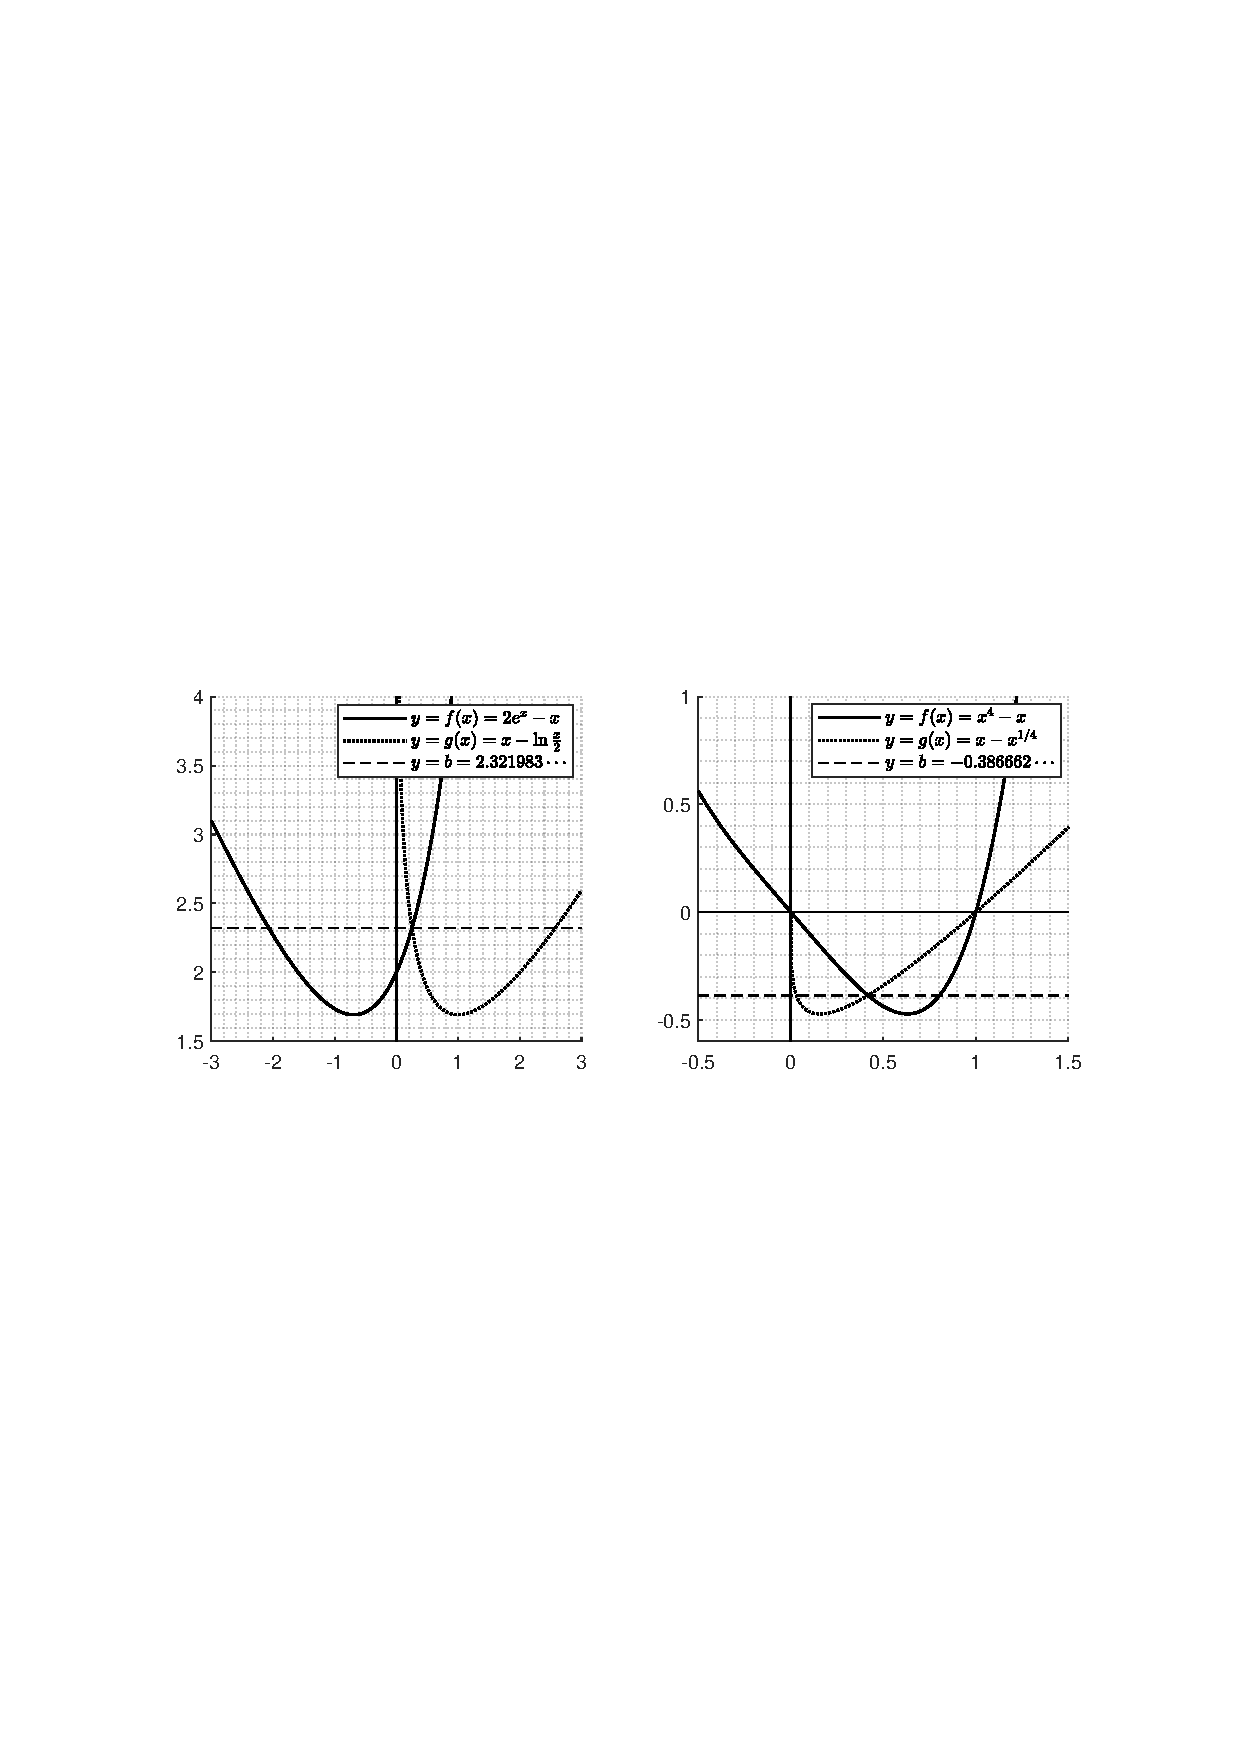
\includegraphics[width=0.95\linewidth]{2022新高考I卷推广}
\end{figure}

\textbf{推广2}\ 设$ f(x)=\dfrac{x}{F(x)},\ g(x)=\dfrac{G(x)}{x} $,其中
$ F(x),\ G(x) $互为反函数,$ f(x),\ g(x) $都有且仅有一个极值点,
且$ y=f(x),\ y=g(x) $至少有一个交点,
那么过其中某个交点的水平直线与$ y=f(x),\ y=g(x) $共有
三个交点,且三个交点横坐标成等比数列。\\
比如$ f(x)=\dfrac{x}{\ln x},\ g(x)=\dfrac{\e^x}{x} $,
那么三个交点横坐标分别为$ x_1=\ln x_2=0.527447\cdots $,
$ x_2=1.694600\cdots $,$ x_3=\e^{x_2}=5.444472\cdots $.
满足$ x_1+x_3=x_2^2 $.

\item (2018,浙江高考)已知函数$ f(x)=\sqrt{x}-\ln x $.\\
(I)若$ f(x) $在$ x_1,x_2\ (x_1\neq x_2) $处的导数相等,证明:$ f(x_1)+f(x_2)>8-8\ln 2 $; \\
(II)若$ a\leq 3-4\ln 2 $,证明:对于任意$ k>0 $,直线$ y=kx+a $与曲线$ y=f(x) $有唯一公共点。 \\
\textbf{解}\ (I)$ f'(x)=\dfrac{1}{2\sqrt{x}}-\dfrac{1}{x},\ f'(4)=0,\  f''(x)=-\dfrac{1}{4x^{3/2}}+\dfrac{1}{x^2},\ f''(16)=0 $,所以$ f'(x) $在$ x=16 $处取得极大值。$ f'(x_1)=f'(x_2),\ 4<x_1<16<x_2 $,
\begin{gather*}
    \dfrac{1}{2\sqrt{x_1}}-\dfrac{1}{x_1}=\dfrac{1}{2\sqrt{x_2}}-\dfrac{1}{x_2} \\ 
    \dfrac{1}{2}\sqrt{x_1x_2}=\sqrt{x_1}+\sqrt{x_2}>
    2\sqrt{\sqrt{x_1}\cdot \sqrt{x_2}}\ 
    \Rightarrow \ 	x_1x_2>16^2=256 \\
    f(x_1)+f(x_2)=\sqrt{x_1}+\sqrt{x_2}-\ln(x_1x_2)
    =\dfrac{1}{2}\sqrt{x_1x_2}-\ln(x_1x_2)
\end{gather*}
令$ g(x)=\dfrac{1}{2}\sqrt{x}-\ln x,\ g'(x)=\dfrac{1}{4\sqrt{x}}-\dfrac{1}{x}=\dfrac{\sqrt{x}-4}{4x},\ g'(16)=0 $,$ g(x) $在$ (16,+\infty) $上单调递增,所以,$ f(x_1)+f(x_2)=g(x_1x_2)>g(256)=8-8\ln 2 $. \medskip \\
(II)\textbf{方法一}\  
$ \sqrt{x}-\ln x=kx+a\ \Rightarrow \ \dfrac{\sqrt{x}-\ln x-a}{x}=k $,
令$ G(x)=\dfrac{\sqrt{x}-\ln x-a}{x}=\dfrac{f(x)-a}{x-0} $,$ G(x) $代表曲线$ y=f(x) $上一点与$ y $轴上的点$ (0,a) $的连线的斜率,$ G'(x)=\dfrac{-\dfrac{1}{2}\sqrt{x}+\ln x+a-1}{x^2}=\dfrac{-g(x)+a-1}{x^2} $,由(I)知,$ g(x) $在$ x=16 $处取得极小值$ 2-4\ln 2 $,$ -g(x)+a-1\leq -(2-4\ln2)+a-1=a-(3-4\ln 2)\leq 0 $,所以$ G'(x)\leq 0 $,$ G(x) $在$ (0,+\infty) $上单调递减,$ \lim\limits_{x\to 0}G(x)=+\infty,\ \lim\limits_{x\to +\infty}G(x)=0 $,根据连续函数的介值定理,$ G(x)=\dfrac{\sqrt{x}-\ln x-a}{x}=k\ (k>0) $有且仅有一个解,即直线$ y=kx+a $与曲线$ y=f(x) $恰好有一个交点。\\
\textbf{方法二}\ 把$ \sqrt{x}-\ln x=kx+a $变形成$ \sqrt{x}-\ln x-kx=a $,记$ h(x)=\sqrt{x}-\ln x-kx $,那么需要证明$ h(x)=a $有且仅有一个解。因为,$ \lim\limits_{x\to 0}h(x)=+\infty,\ \lim\limits_{x\to +\infty}h(x)=-\infty $(当$ x $足够大时,$ \sqrt{x} $的增长速度总会慢于$ kx $),根据连续函数的介值定理,任意$ a\in \textbf{R} $(\textbf{R}为实数集),方程$ h(x)=a $至少存在一个解。下面需要证明解的唯一性。$ h'(x)=\dfrac{1}{2\sqrt{x}}-\dfrac{1}{x}-k=\dfrac{\sqrt{x}-2-2kx}{2x},\ \sqrt{x}-2-2kx=0,\ \Delta=1-16k $. \\
\mycircled{1}若$ k\geq \dfrac{1}{16},\ \Delta\leq 0 $,则$ h'(x)\leq 0 $,$ h(x) $在$ (0,+\infty) $上单调递减,$ h(x)=a $有唯一解。\\
\mycircled{2}若$ 0<k<\dfrac{1}{16} $,$ h(x) $在$ (0,+\infty) $上有两个极值点$ t_{1,2}= \left(\dfrac{1\pm\sqrt{1-16k}}{4k}\right)^2 $,如果直接把$ t_{1,2} $代入$ h(x) $,则$ h(t_{1,2}) $的表达式相当复杂,难以判断与$ 3-4\ln2 $的相对大小,进而难以判断$ h(x)=a $的解的数量,所以要换个思路。先考虑极小值点$ t_1 $,由$ \sqrt{t_1}-2-2kt_1=0 $可得:$ kt_1=\dfrac{1}{2}\sqrt{t_1}-1 $,那么
\begin{align*}
    h(t_1)=&\ \sqrt{t_1}-\ln t_1-kt_1=\sqrt{t_1}-\ln t_1-(\dfrac{1}{2}\sqrt{t_1}-1)
    \\ =&\ \dfrac{1}{2}\sqrt{t_1}-\ln t_1+1\geq (2-4\ln 2)+1=3-4\ln 2
\end{align*}
其中的“=”能否取到,取决于$ t_1 $能否等于$ 16 $,不妨令$ t_1=\left(\dfrac{1-\sqrt{1-16k}}{4k}\right)^2=16 $,解得$ k=\dfrac{1}{16} $.现在$ 0<k<\dfrac{1}{16} $,所以$ t_1\neq 16,\ h(t_1)>3-4\ln 2 $.因为$ h(x) $在$ (0,t_1) $和$ (t_2,+\infty) $上分别单调递减,在$ (t_1,t_2) $上单调递增,$ h(t_2)>h(t_1)>3-4\ln 2 $,所以$ h(x)=a\ (a\leq 3-4\ln 2) $在区间$ (0,t_2) $上无解,在区间$ (t_2,+\infty) $上有唯一解。\\
\textbf{注}:\ $ 3-4\ln 2 $这个值,实际上是曲线$ y=f(x) $的切线在$ y $轴上截距的最小值,计算如下:过点$ (x_0,f(x_0)) $的切线方程为$ y-f(x_0)=f'(x_0)(x-x_0) $,在$ y $轴上的截距为$ b=f(x_0)-x_0f'(x_0)=\dfrac{1}{2}\sqrt{x_0}-\ln x_0+1=g(x_0)+1\geq (2-4\ln 2)+1=3-4\ln2 $.截距的最小值在$ x_0=16 $时取得,而$ f''(x_0)=f''(16)=0 $,即$ x_0=16 $是$ f(x) $的拐点。换言之,拐点处的切线能让切线截距达到极值。原因如下:令$ \phi(x)=f(x)-xf'(x) $,则
\begin{gather*}
    \phi'(x)=f'(x)-[f'(x)+xf''(x)]=-xf''(x) \\
    \phi'(x)=0\q \Rightarrow \q x=0\ \text{或}\ f''(x)=0
\end{gather*}

如果某条直线在$ y $轴上截距小于$ 3-4\ln2 $,则不可能是$ y=f(x) $的切线,而只能与$ y=f(x) $相交,但这样无法判断交点的数量。\\
\\
按照上面的思想,可以编制如下题目:\\
(I)求$ y=f(x)=\dfrac{x}{x^2+1} $的切线在$ y $轴上的截距的取值范围。\\
\textbf{解}\ 令$ \phi(x)=f(x)-xf'(x) $,则
\begin{gather*}
    \phi'(x)=-xf''(x)=\dfrac{2x^2(3-x^2)}{(x^2+1)^3},\ 
\end{gather*}
$ \phi'(\pm\sqrt{3})=0,\ \phi(\pm\sqrt{3})=\pm\dfrac{3\sqrt{3}}{8} $,于是,截距的范围是$ \left[-\dfrac{3\sqrt{3}}{8},\dfrac{3\sqrt{3}}{8}\right] $.对于直线$ y=kx+a $,当$ a $超过切线截距的范围,那么直线与$ y=\dfrac{x}{x^2+1}  $至多有一个交点(作为证明题,读者自行完成)。\\
(II)求$ y=f(x)=\dfrac{x^2}{x^4+1} $的切线在$ y $轴上的截距的取值范围。(计算量较大,可借助软件完成,不适合拿来考试)。\\
\textbf{解}\ 令$ \phi(x)=f(x)-xf'(x) $,则
\begin{gather*}
    \phi'(x)=-xf''(x)=\dfrac{-2x(3x^8-12x^4+1)}{(x^4+1)^3},\q
    \phi'\left(\sqrt[4]{2\pm \dfrac{\sqrt{33}}{3}}\right)=0
\end{gather*}
于是,截距的范围是
\begin{gather*}
    \left[\dfrac{1}{32}(-1-\sqrt{33})\sqrt{18+3\sqrt{33}},\dfrac{1}{32}
    (-1+\sqrt{33})\sqrt{18+3\sqrt{33}}\right]\approx [-0.184504, 0.880086]
\end{gather*}

\item 设$ 0<x_1<x_2 $,求证:
\begin{gather}\label{对数均值不等式左半部分}
	\sqrt{x_1x_2}<\dfrac{x_2-x_1}{\ln x_2-\ln x_1}	
\end{gather} \\
\textbf{证}\ 原不等式两边同除$ x_1 $,有$ \sqrt{\dfrac{x_2}{x_1}}<
\dfrac{\dfrac{x_2}{x_1}-1}{\ln\dfrac{x_2}{x_1}} $,令$ t=\dfrac{x_2}{x_1}>1 $,
则要证$ \sqrt{t}<\dfrac{t-1}{\ln t} $,如果直接将$ \sqrt{t}-
\dfrac{t-1}{\ln t}$对$ t $求导,则计算量太大,应当尽量避免使用两个函数乘或除的
求导法则。设$ f(t)=\ln t-\sqrt{t}+\dfrac{1}{\sqrt{t}}$,
则$ f'(t)=-\dfrac{(\sqrt{t}-1)^2}{2t^{3/2}}<0 $.所以,$ f(t)<f(1)=0 $,即
\begin{align}\label{lnt<sqrt(t)-1/sqrt(t)}
	\ln t<\sqrt{t}-\dfrac{1}{\sqrt{t}} \quad (t>1)
\end{align}
把其中的$ t $换成$ t^2 $,有
\begin{gather}\label{不等式2lnt<t-1/t}
	 2\ln t<t-\dfrac{1}{t}\quad (t>1) 
\end{gather}

\item (2018,全国I卷)已知函数$ f(x)=\dfrac{1}{x}-x+a\ln x $.\\
(I)讨论$ f(x) $的单调性;\\
(II)若$ f(x) $存在两个极值点$ x_1,x_2 $,证明:
$ \dfrac{f(x_2)-f(x_1)}{x_2-x_1}<a-2 $. \\
\textbf{解}\ (I)略 \\
(II) $ f'(x)=-\dfrac{1}{x^2}-1+\dfrac{a}{x}=-\dfrac{1}{x^2}(x^2-ax+1) $,令$ x^2-ax+1=0,\ \Delta=a^2-4>0 $,由韦达定理,$ x_1+x_2=a>0,\ x_1x_2=1 $,所以$ a>2 $. 不妨设$ 0<x_1<1<x_2 $,又有
\begin{align*}
	\dfrac{f(x_2)-f(x_1)}{x_2-x_1}=-\dfrac{1}{x_1x_2}-1+
	a\dfrac{\ln x_2-\ln x_1}{x_2-x_1} 
	=-2+\dfrac{a(\ln x_2-\ln \dfrac{1}{x_2})}
	{x_2-\dfrac{1}{x_2}} 	
	=-2+\dfrac{2a\ln x_2}{x_2-\dfrac{1}{x_2}}
\end{align*}
根据(\ref{不等式2lnt<t-1/t})式,(当然可以直接求导证明),有$ 0<2\ln x_2<x_2-\dfrac{1}{x_2} $,所以$ \dfrac{2a\ln x_2}{x_2-\dfrac{1}{x_2}}<a $,原不等式成立。

有的读者可能会想到使用拉格朗日中值定理,$ \dfrac{f(x_2)-f(x_1)}{x_2-x_1}=f'(\xi),\  \xi\in(x_1,x_2) $,而$f'(\xi) $肯定不超过$ f'(x) $在区间$ [x_1,x_2] $上的最大值,$ f''(x)=\dfrac{2-ax}{x^3} $,其零点是$ x_0=\dfrac{2}{a}\in (x_1,x_2)=\left(\dfrac{a-\sqrt{a^2-4}}{2},\dfrac{a+\sqrt{a^2-4}}{2}\right)=\left(\dfrac{2}{a+\sqrt{a^2-4}},\dfrac{2}{a-\sqrt{a^2-4}}\right) $,所以$ f'(x) $在$ x_0 $处取得极大值,但是$ f'(x_0)=\dfrac{a^2}{4}-1>a-2 $,缩放过头了,这样做行不通。

\item 综合(\ref{对数均值不等式左半部分})和(\ref{对数均值不等式右半部分})式,对任意两个不等的正实数$ x_1,x_2 $,有
\begin{align} \label{对数割线斜率不等式}
	\sqrt{x_1x_2}<\dfrac{x_2-x_1}{\ln x_2-\ln x_1}<\dfrac{x_1+x_2}{2}
\end{align}
其中,$ \dfrac{x_2-x_1}{\ln x_2-\ln x_1} $被称为对数平均值。请读者自行思考,为什么上式不要求$ x_1>1,x_2>1 $.把上式中的$ x_1 $换成$ \e^{x_1} $,
$ x_2 $换成$ \e^{x_2} $,可得:
\begin{align*}
	\e^{\frac{x_1+x_2}{2}}<\dfrac{\e^{x_2}-\e^{x_1}}{x_2-x_1}<
	\dfrac{\e^{x_1}+\e^{x_2}}{2}
\end{align*}
2013年陕西高考考察了以上不等式的右侧。只需证明
\begin{gather*}
	\e^{x_2}-\e^{x_1}<\dfrac{1}{2}(x_2-x_1)(\e^{x_1}+\e^{x_2}) \\
	\e^{x_2-x_1}-1<\dfrac{1}{2}(x_2-x_1)(\e^{x_2-x_1}+1) 
\end{gather*}
令$ t=x_2-x_1>0 $,证明$ \e^t-1-\dfrac{1}{2}t(\e^t+1)<0 $即可。2014年天津高考考察了函数$ \dfrac{t(\e^t+1)}{\e^t-1}\ (t>0) $的单调性。

$ \bullet $ 将(\ref{2(t-1)/(t+1)<lnt})式和(\ref{lnt<sqrt(t)-1/sqrt(t)})式合在一起,
\begin{align}\label{lnt不等式链t>1}
	\dfrac{2(t-1)}{t+1}<\ln t<\sqrt{t}-\dfrac{1}{\sqrt{t}}=
	\dfrac{t-1}{\sqrt{t}}<t-1 \quad (t>1)
\end{align}
如果$ 0<t<1 $,那么以上不等式链反向:
\begin{align}\label{lnt不等式链0<t<1}
	\dfrac{2(t-1)}{t+1}>t-1>\ln t>\sqrt{t}-\dfrac{1}{\sqrt{t}}=
	\dfrac{t-1}{\sqrt{t}} \quad (0<t<1)
\end{align}
将(\ref{lnt不等式链t>1})式中的$ t $换成$ t+1 $,有
\begin{align}\label{ln(1+t)不等式链t>0}
	\dfrac{2t}{t+2}=\dfrac{t}{1+\dfrac{1}{2}t}<\ln(t+1)<\dfrac{t}{\sqrt{t+1}}<t \quad (t>0)
\end{align}
如果$ -1<t<0 $,那么以上不等式链反向:
\begin{align}\label{ln(1+t)不等式链-1<t<0}
	\dfrac{2t}{t+2}=\dfrac{t}{1+\dfrac{1}{2}t}>t>\ln(t+1)>\dfrac{t}{\sqrt{t+1}} \quad (-1<t<0 )
\end{align}
%\\
%\item 将(\ref{lnt<sqrt(t)-1/sqrt(t)})式中的$ t $换成$ t^{2n},\ n\in \textbf{N}^+ $,有
%\begin{align*}
%	2n\ln t<&\ t^n-\dfrac{1}{t^n}, \quad 
%	\ln t<\dfrac{1}{2n}\left(t^n-\dfrac{1}{t^n}\right) \quad
%	(t>1) \\
%	2n\ln t>&\ t^n-\dfrac{1}{t^n}, \quad
%	\ln t>\dfrac{1}{2n}\left(t^n-\dfrac{1}{t^n}\right) \quad
%	(0<t<1) 
%\end{align*}

% TianJin2010Jizhipianyi.m
\item (2010,天津高考)已知函数$ f(x)=x\e^{-x}\ (x\in \textbf{R}) $ \\
(1) 求函数$ f(x) $的单调区间和极值;\\
(2) 已知函数$ y=g(x) $的图像与函数$ y=f(x) $的图像关于直线$ x=1 $对称,证明:
当$ x>1 $时,$ f(x)>g(x) $;\\
(3) 若$ x_1\neq x_2 $,且$ f(x_1)=f(x_2) $ ,证明:$ x_1+x_2>2 $。\\
\textbf{解}\ (1)\ $ f'(x)=(1-x)\e^{-x} $,$ f(x) $在$ (0,1) $上单调递增,在$ (1,+\infty) $上单调递减,在$ x=1 $处取得极大值$ \dfrac{1}{\e} $. \\
(2)\ $ g(x)=f(2-x)=(2-x)\e^{x-2} $,令$ h(x)=f(x)-g(x)=x\e^{-x}-(2-x)\e^{x-2} $,$ h'(x)=(x-1)(\e^{2x-2}-1)\e^{-x}\geq 0 $,$ h(x) $在\textbf{R}上单调递增。当$ x>1 $时,$ h(x)>h(1)=0,\ f(x)>g(x) $. \\
(3)\ \textbf{方法一}\ 设$ 0<x_1<1<x_2 $,因为$ f(x_1)=f(x_2)>g(x_2)=f(2-x_2) $,
又有$ 2-x_2<1 $,且$ f(x) $在$ (-\infty,1) $上单调递增,所以$ x_1>2-x_2,\ x_1+x_2>2 $. \\
\begin{figure}[h]
	\centering
	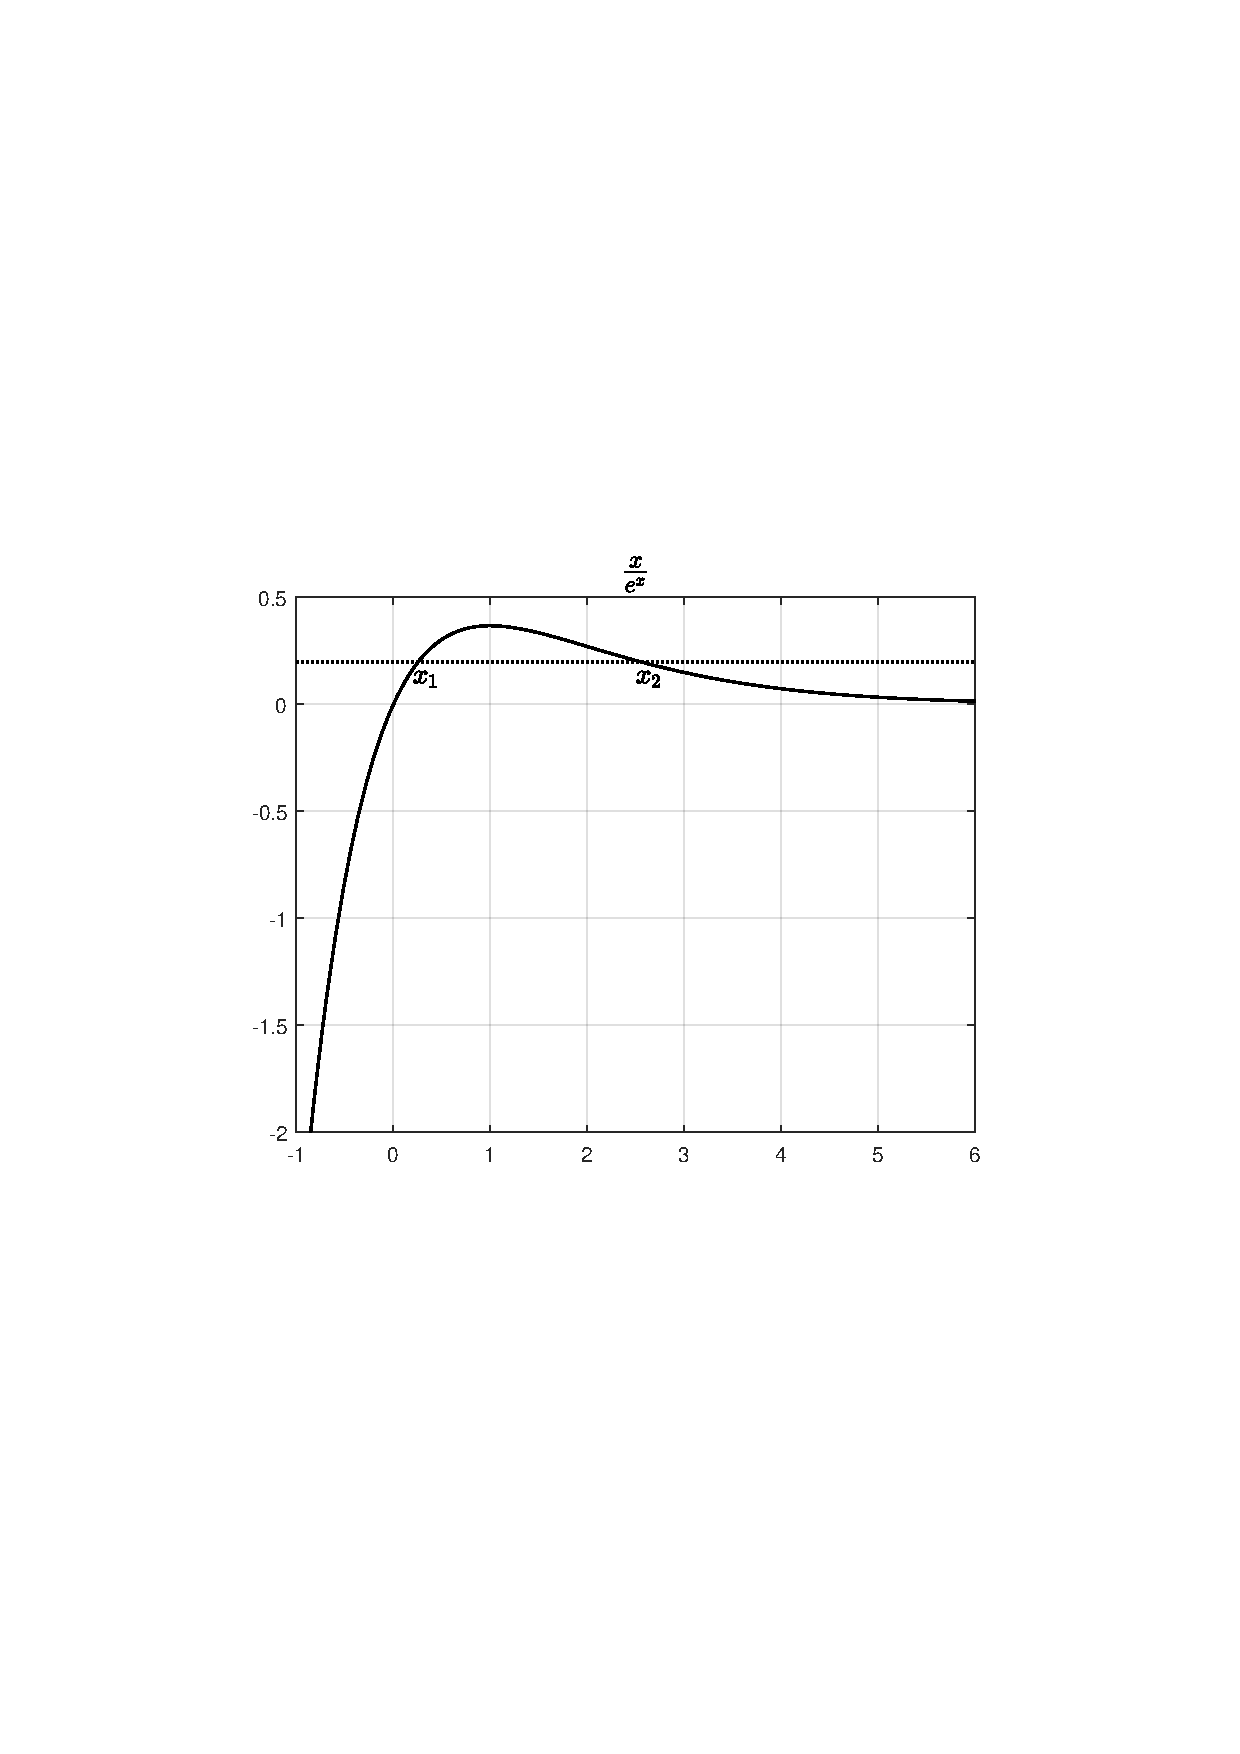
\includegraphics[width=0.4\linewidth]{2010天津高考}
\end{figure}
\textbf{注}:本题就是“极值点偏移”问题的典型代表,所谓极值点偏移是指函数图像在极值点左右两侧不对称。如果$ f(x) $的图像在极值点左右两侧是对称的,那么$ x_1+x_2 $等于极值点横坐标的两倍。现在$ f(x)=x\e^{-x} $,在$ x=1 $左侧,图像陡峭;在$ x=1 $右侧,图像平缓,显然有$ x_2-1>1-x_1 $,即$ x_1+x_2>2 $. 

本题第(2)和(3)问展示的方法也是解决极值点偏移问题的首选方案。如果极值点横坐标是$ x_0 $,那么构造函数$ h(x)=f(x)-f(2x_0-x) $,或者$ h(x)=f(x_0+x)-f(x_0-x) $,然后求出$ h'(x) $. 一般而言,当$ x>x_0 $时,$ h(x) $是单调的。\\
\textbf{方法二}\ 令$ H(x)=\dfrac{f(2-x)}{f(x)}=\dfrac{2-x}{x}\e^{2x-2}\ (x>0) $,
则$ H'(x)=-\dfrac{2(x-1)^2}{x^2}\e^{2x-2}\leq 0 $,同样设$ 0<x_1<1<x_2 $,那么$ H(x_2)<H(x_1) $,
\begin{gather*}
	\dfrac{(2-x_2)x_2\e^{2x_2-2}}{x_2^2} <
	\dfrac{(2-x_1)x_1\e^{2x_1-2}}{x_1^2} 
\end{gather*}
又因为$ f(x_1)=f(x_2) $,所以	$ \dfrac{\e^{2x_1-2}}{x_1^2}=\dfrac{\e^{2x_2-2}}{x_2^2} $,于是
\begin{gather*}
    (2-x_2)x_2<(2-x_1)x_1 \\
	2x_2-x_2^2-(2x_1-x_1^2)=(x_2-x_1)[2-(x_1+x_2)]< 0 \\
	2<x_1+x_2
\end{gather*} 

\item (2014,天津高考)已知函数$ f(x)=x-a\e^{x}\ (x\in \textbf{R}) $,$ f(x) $
有两个零点$ x_1,x_2\ (x_1<x_2) $. \\
(1) 求$ a $的取值范围;\\
(2) 证明:$ \dfrac{x_2}{x_1} $随着$ a $的减小而增大;\\
(3) 证明:$ x_1+x_2 $随着$ a $的减小而增大。\\
\textbf{解}\ (1)\textbf{方法一}:等价于方程$ \dfrac{1}{a}x=\e^x $有两个解,因为$ \e^x\geq \e x $\footnote{\q $ \e^x\geq 1+x,\ \e^{x-1}\geq x $,两边同乘$ \e $可得$ \e^x\geq \e x $. },而直线$ y=\e x $过原点,且与$ y=\e^x $相切。所以,只要$ \dfrac{1}{a}> \e $,$ y=\dfrac{1}{a}x $与$ y=\e^x $就有两个交点,于是$ 0<a<\dfrac{1}{\e} $. \\
\textbf{方法二}:等价于$ \dfrac{x}{\e^x}=a $有两个不等根,这就与上面2010年的天津高考题一样,求出$ \dfrac{x}{\e^x} $的极值即可。\\
(2) 显然有$ 0<x_1<1<x_2 $,根据$ \dfrac{x}{\e^x} $的单调性,
随着$ a $的减小,$ x_1 $减小,$ x_2 $增加,$ \dfrac{x_2}{x_1} $
当然会增加。\\
(3)  用类似(\ref{lnx_x极值偏移1})式和(\ref{lnx_x极值偏移2})式的方法,
\begin{gather*}
	\dfrac{x_1}{\e^{x_1}}=\dfrac{x_2}{\e^{x_2}}=
	\dfrac{x_2+x_1}{\e^{x_2}+\e^{x_1}}=
	\dfrac{x_2-x_1}{\e^{x_2}-\e^{x_1}} \\
	x_1+x_2=(x_2-x_1)\dfrac{\e^{x_2}+\e^{x_1}}{\e^{x_2}-\e^{x_1}} 
	=(x_2-x_1)\dfrac{\e^{x_2-x_1}+1}{\e^{x_2-x_1}-1}
\end{gather*}
令$ t=x_2-x_1>0,\ g(t)=\dfrac{t(\e^t+1)}{\e^t-1} $,则$ g'(t)=\dfrac{\e^{2t}-2te^t-1}{(\e^t-1)^2} $,再令$ h(t)=\e^{2t}-2te^t-1\ (t>0) $,则$ h'(t)=2e^t[\e^t-(t+1)]>0 $,所以$ h(t)>h(0)=0,\ g'(t)=\dfrac{h(t)}{(\e^t-1)^2}>0,\ g(t) $在$ (0,+\infty) $上单调递增。显然,随着$ a $的减小,$ t=x_2-x_1 $会增加,$ x_1+x_2=g(t) $也增加。

如果令$ u=\e^t>1 $,那么$ t=\ln u$ ,令$ \varphi(u)=g(\ln u)=\dfrac{(u+1)\ln u}{u-1},\ \varphi'(u)=\dfrac{u-\dfrac{1}{u}-2\ln u}{(u-1)^2} $,根据(\ref{不等式2lnt<t-1/t})式,$ u-\dfrac{1}{u}>2\ln u\ (u>1) $,所以$ \varphi'(u)>0,\ \varphi(u) $在$ (1,+\infty) $上单调递增,同样能说明$ x_1+x_2 $随着$ a $的减小而增大。

% Tianjin2015.m
\item (2015,天津高考)已知函数$ f(x)=nx-x^n,\ x\in \textbf{R} $其中,
$ n\in \textbf{N}^+ $且$ n\geq 2 $.\\
(I)讨论$ f(x) $的单调性;\\
(II)设曲线$ y=f(x) $与$ x $轴正半轴的交点为$ P $,曲线在点$ P $
处的切线方程为$ y=g(x) $,求证:对于任意的正实数$ x $,都有
$ f(x)\leq g(x) $;\\
(III)若关于$ x $的方程$ f(x)=a $($ a $为实数)有两个正实数根
$ x_1,\ x_2 $,求证:$ |x_2-x_1|<\dfrac{a}{1-n}+2 $. \\
\textbf{解}\ (1) $ f'(x)=n(1-x^{n-1}) $. $ f(x) $在
$ (-\infty,1) $上单调递增,在$ (1,+\infty) $上单调递减。\\
(2) 令$ x_0=n^{\frac{1}{n-1}} $,则$ P(x_0,0) $,
$ g(x)=(n-nx_0^{n-1})(x-x_0)=(n-n^2)(x-x_0) $,\\
令$ h(x)=g(x)-f(x) $,则$ h'(x)=g'(x)-f'(x)=(n-n^2)-
(n-nx^{n-1})=n(x^{n-1}-n) $,所以,$ h(x) $在
$ (0,x_0) $上单调递减,在$ (x_0,+\infty) $上单调递增,
$ h(x)=g(x)-f(x)\geq h(x_0)=0\ (x>0) $. \\
(3) \textbf{方法一}\ 切线法。
\begin{figure}[H]
    \centering
    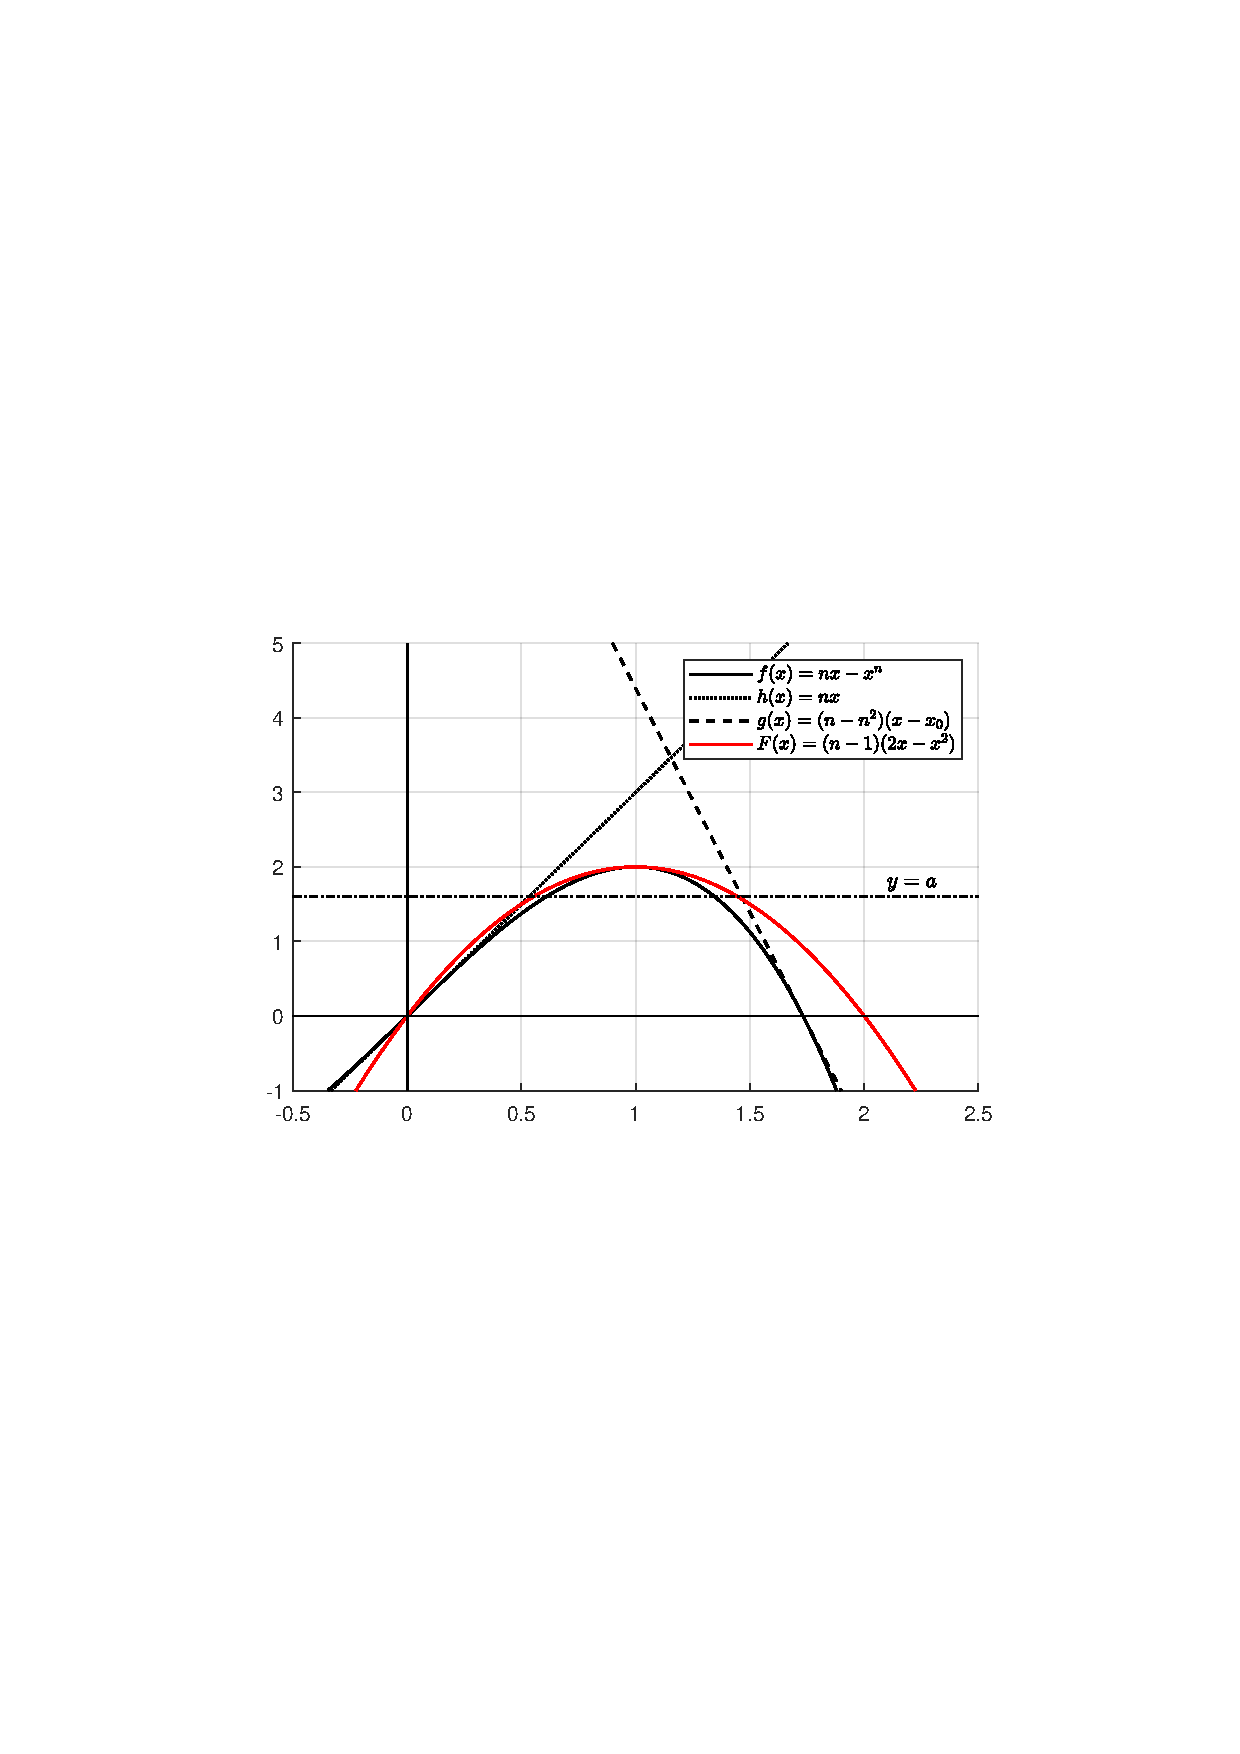
\includegraphics[width=0.6\linewidth]{2015天津高考}
\end{figure}
$ f(x) $在$ x=1 $处取得极大值$ n-1 $,所以$ 0<a<n-1 $.
不妨设$ 0<x_1<1<x_2<x_0=n^{\frac{1}{n-1}} $. $ f(x) $
在$ x=0 $处的切线的切线为$ y=h(x)=nx $,显然,
$ h(x)\geq f(x) $在$ (0,+\infty) $上恒成立,
设$ h(u_1)=f(x_1)=f(x_2)=g(x_2)=a $,
可解得$ u_1=\dfrac{a}{n} $,$ u_2=\dfrac{a}{n(1-n)}+x_0 $,
因为$ 0<u_1<x_1<1<x_2<u_2<x_0 $,所以,
\begin{gather*}
    |x_2-x_1|<u_2-u_1=\frac{a}{1-n}+x_0
\end{gather*}
下面证明$ x_0\leq 2 $.等价于证明$ 2^{n-1}\geq n\ 
(n\geq 2) $,可以使用数学归纳法或者二项式定理,比如
$ 2^{n-1}=(1+1)^{n-1}\geq 1+C_{n-1}^1=1+(n-1)=n $. 证毕。\\
\textbf{方法二}\ 抛物线法。考虑过原点且顶点与$ f(x) $的极大值点重合
的抛物线$ F(x)=(n-1)(2x-x^2) $,容易证明(略):$ F(x)\geq f(x) $
在$ (0,2) $上恒成立。设$ v_1<v_2 $,
$ F(v_1)=f(x_1)=f(x_2)=F(v_2)=a $,那么,
\begin{gather*}
    |x_2-x_1|<v_2-v_1=\sqrt{4+\dfrac{4a}{1-n}}=
    2\sqrt{1+\dfrac{a}{1-n}}<2\left[1+\frac{a}{2(1-n)}\right]
    =2+\dfrac{a}{1-n}
\end{gather*}
以上使用了不等式$ \sqrt{1+x}<1+\dfrac{1}{2}x\ (x\geq -1,x\neq 0) $.证毕。\\
\textbf{注1}:证明$ x_0\leq 2 $也可以使用对数求导法. 
令$ \varphi(x)=x^{\frac{1}{x-1}}\ (x>1) $,
$ \ln\varphi(x)=\dfrac{\ln x}{x-1} $,两边求导,
\begin{gather*}
    \frac{\varphi'(x)}{\varphi(x)}=
    \dfrac{1-\frac{1}{x}-\ln x}{(x-1)^2},\q 
    \varphi'(x)=x^{\frac{1}{x-1}} 
    \dfrac{1-\frac{1}{x}-\ln x}{(x-1)^2} 
\end{gather*}
容易证明,$ \dfrac{1}{x}+\ln x $在$ (0,+\infty) $上的极小值是1(当$ x=1 $),
所以,$ \varphi'(x)<0 $,$ \varphi(x) $在
$ (1,+\infty) $上单调递减。$ n\geq 2,\ x_0=\varphi(n)\leq 
\varphi(2)=2 $. 另外,$ \lim\limits_{n\to+\infty}n^{\frac{1}{n-1}}=1 $.\\
\textbf{注2}:请读者自行证明:当$ n\geq 3 $时,$ x_0<x_1+x_2<2 $. \\
提示:要证$ x_1+x_2<2 $,只需证$ x>1 $时,$ f(x)<f(2-x) $;
要证$ 0<x_1+x_2 $,可考虑抛物线$ y=\dfrac{n-1}{x_0-1}x(x_0-x) $,
这条抛物线过原点、$ P(x_0,0) $点和$ f(x) $的极大值点$ (1,n-1) $.

% XinGaoKao_I_2021.m
\item (2021,新高考全国I卷)已知函数$ f(x)=x(1-\ln x)\ (x>0) $ \\
(1) 讨论$ f(x) $的单调性;\\
(2) 设$ a,b $为两个不相等的正实数,且$ b\ln a-a\ln b=a-b $,证明:
$ 2< \dfrac{1}{a}+\dfrac{1}{b}<\e $.\\
\textbf{解}\ (1)\ $ f'(x)=-\ln x $,所以$ f(x) $在$ (0,1) $上单调递增,
在$ (1,+\infty) $上单调递减,在$ x=1 $处取得极大值1.
\begin{figure}[H]
	\centering
	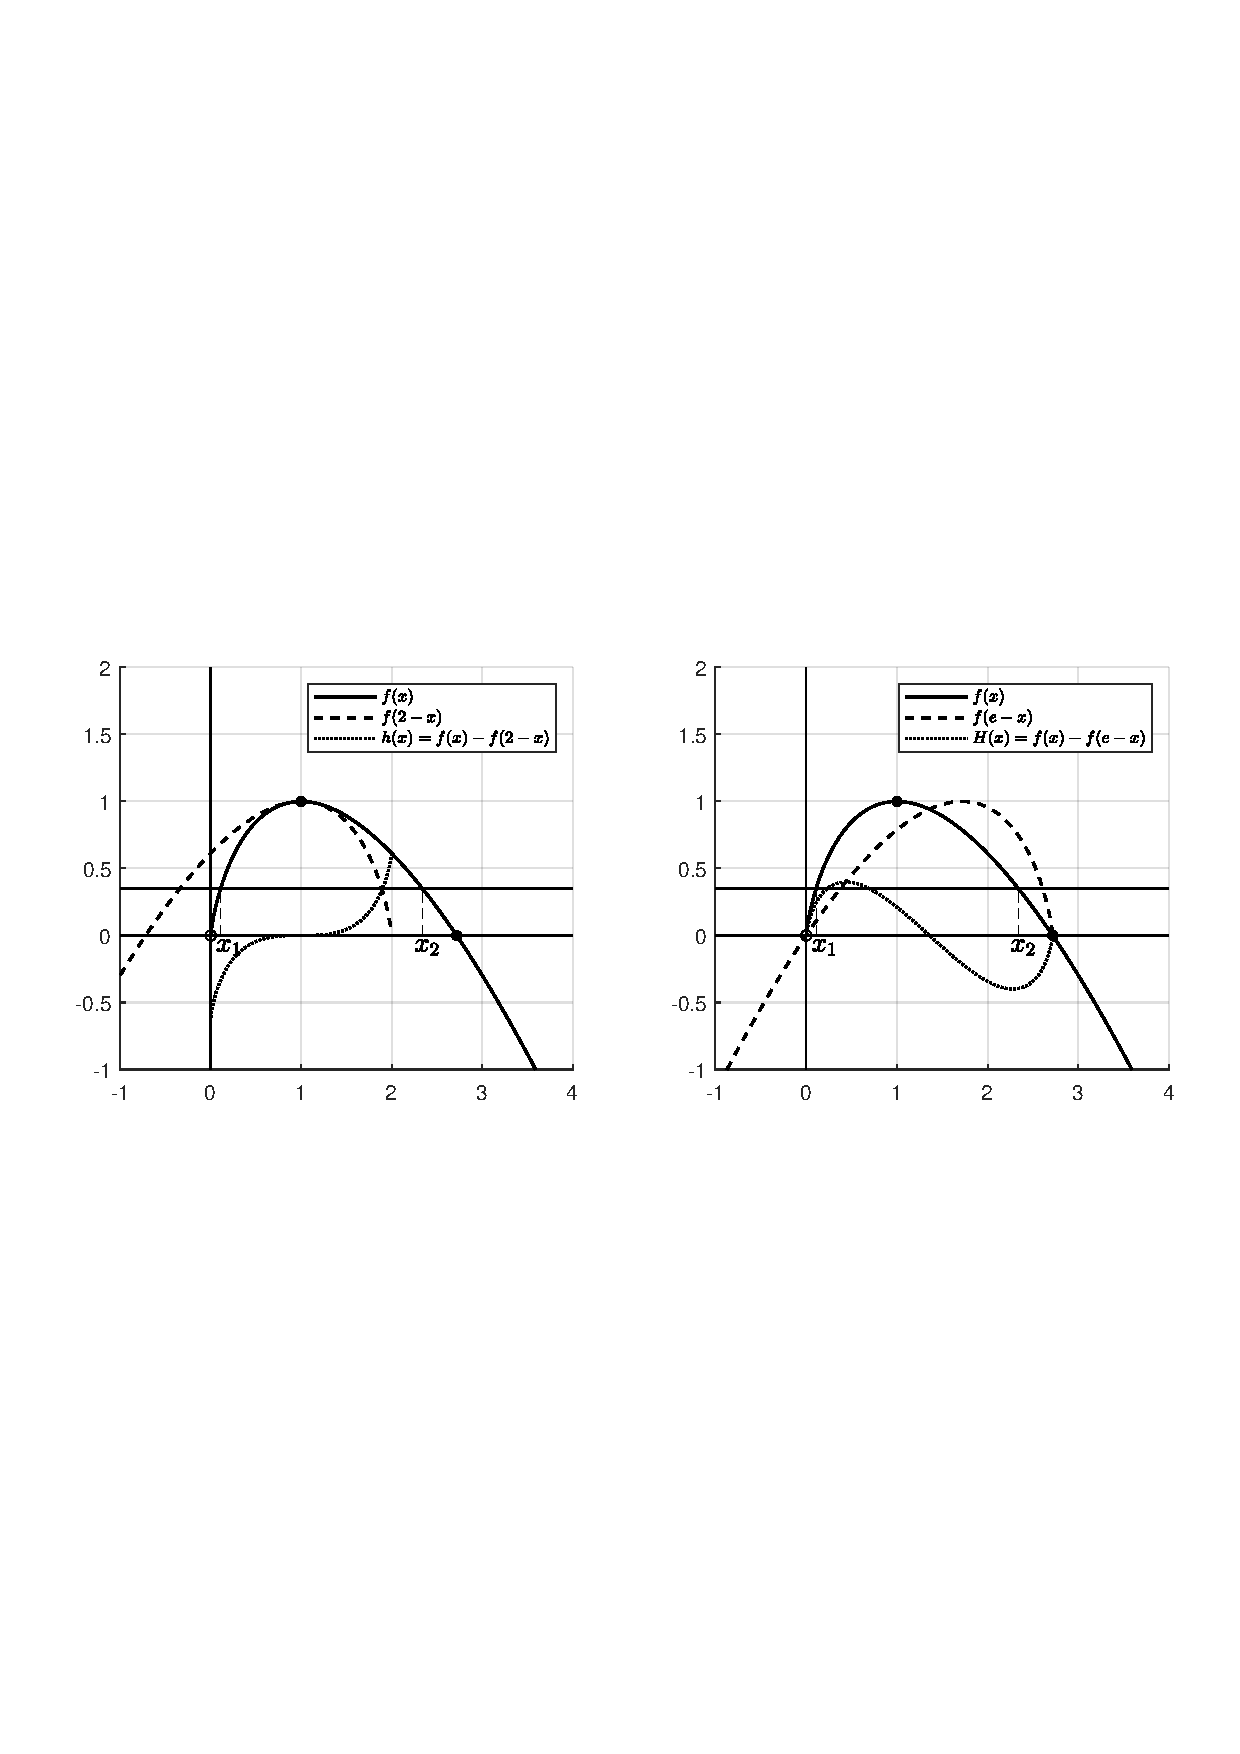
\includegraphics[width=0.9\linewidth]{2021新高考全国I卷图1}
\end{figure} 
\noindent (2) 令$ x_1=\dfrac{1}{a},\ x_2=\dfrac{1}{b} $,则$ b\ln a-a\ln b=a-b $可化为$ x_1(1-\ln x_1)=x_2(1-\ln x_2),\ f(x_1)=f(x_2) $,等价于证明$ 2<x_1+x_2<\e $,此题也属于极值点偏移问题。\\
证明$ x_1+x_2>2 $的\textbf{方法一}:
令$ h(x)=f(x)-f(2-x)=x(1-\ln x)-(2-x)[1-\ln(2-x)],\ (0<x<2) $,则$ h'(x)=-\ln[x(2-x)]\geq 0 $,$ h(x) $在$ (0,2) $上单调递增。所以,当$ 0<x<1 $时,$ h(x)<h(1)=0,\ f(x)<f(2-x) $,当$ 1<x<2 $时,$ h(x)>h(1)=0,\ f(x)>f(2-x) $.不妨设$ 0<x_1<1<x_2<\e $,如果$ x_2\in(1,2) $,那么$ h(x_2)=f(x_2)-f(2-x_2)>0,\ f(x_2)>f(2-x_2),\ f(x_2)=f(x_1)>f(2-x_2) $,因为$ 2-x_2\in(0,1),\  f(x) $在$ (0,1) $上单调递增,所以$ x_1>2-x_2,\ x_1+x_2 >2 $.如果$ x_2\in[2,\e) $,当然也有$ x_1+x_2 >2 $.

上面按$ x_2 $是否小于2进行了分类,事实上也可以不分类,因为
$ h(x_1)=f(x_1)-f(2-x_1)<0,\ f(x_1)<f(2-x_1),\ f(x_1)=f(x_2)<f(2-x_1),\ x_2\in (1,\e), 2-x_1\in (1,2)\subset(1,\e) $,同时,$ f(x) $在$ (1,\e) $上单调递减,所以$ x_2>2-x_1,\ x_1+x_2 >2 $.

证明$ x_1+x_2>2 $的\textbf{方法二}:构造经过$ f(x) $的极大值点$ (1,1) $且以
$ x=1 $为对称轴的抛物线$ p(x)=-A(x-1)^2+1 $,同时还让抛物线满足
$ p''(1)=f''(1)=-1 $,解得$ A=\dfrac{1}{2} $,于是
$ p(x)=-\dfrac{1}{2}(x-1)^2+1 $. 让$ p''(1)=f''(1) $的目的是:
当$ x\in(0,1) $时,$ p(x)>f(x) $;当$ x\in(1,+\infty) $时,
$ p(x)<f(x) $.(建议读者用绘图软件画一画$ y=-\dfrac{1}{2.5}(x-1)^2+1 $
和$ y=-\dfrac{1}{1.5}(x-1)^2+1 $的图像,与$ f(x),\ p(x) $做对比)。
设$ p(x_1')=f(x_1)=p(x_2')=f(x_2)=y_0\in(0,1) $,
那么$ x_1'<x_1<1<x_2'<x_2 $,于是$ x_1+x_2>x_1'+x_2'=2 $.
(因为抛物线$ p(x) $的对称轴是$ x=1 $,所以$ x_1'+x_2'=2 $). 

证明$ x_1+x_2<\e $的\textbf{方法一}:令$ H(x)=f(x)-f(\e-x),\ x\in (0,\e) $,则$ H'(x)=-\ln[x(\e-x)] $,当$ x\in \left(0,\dfrac{\e-\sqrt{\e^2-4}}{2}\right)\cup\left(\dfrac{\e+\sqrt{\e^2-4}}{2},\e\right) $时,$ H'(x)>0,\ H(x) $单调递增,当$ x\in \left(\dfrac{\e-\sqrt{\e^2-4}}{2},\dfrac{\e+\sqrt{\e^2-4}}{2}\right) $时,$ H'(x)<0,\ H(x) $单调递减。根据(\ref{limit_xlnx=0})式,$ \lim\limits_{x\to 0} x\ln x=0 $,所以,$ \lim\limits_{x\to 0} f(x)=0,\ \lim\limits_{x\to 0} H(x)=0 $. 显然有$ H(\dfrac{\e}{2})=0 $,于是当$ x\in (0,\dfrac{\e}{2}) $时,$ H(x)>0,\ f(x)>f(\e-x) $;当$ x\in (\dfrac{\e}{2},\e) $时,$ H(x)<0,\ f(x)<f(\e-x) $. 因为$ x_1\in(0,1) $,所以$ H(x_1)=f(x_1)-f(\e-x_1)>0,\ f(x_1)>f(\e-x_1),f(x_1)=f(x_2)>f(\e-x_1) $,
$ x_2\in(1,\e),\ \e-x_1\in (\e-1,\e)\subset(1,\e) $,再根据$ f(x) $在$ (1,\e) $上单调递减,所以$ x_2<\e-x_1,\ x_1+x_2<\e $.
\begin{figure}[h]
	\centering
	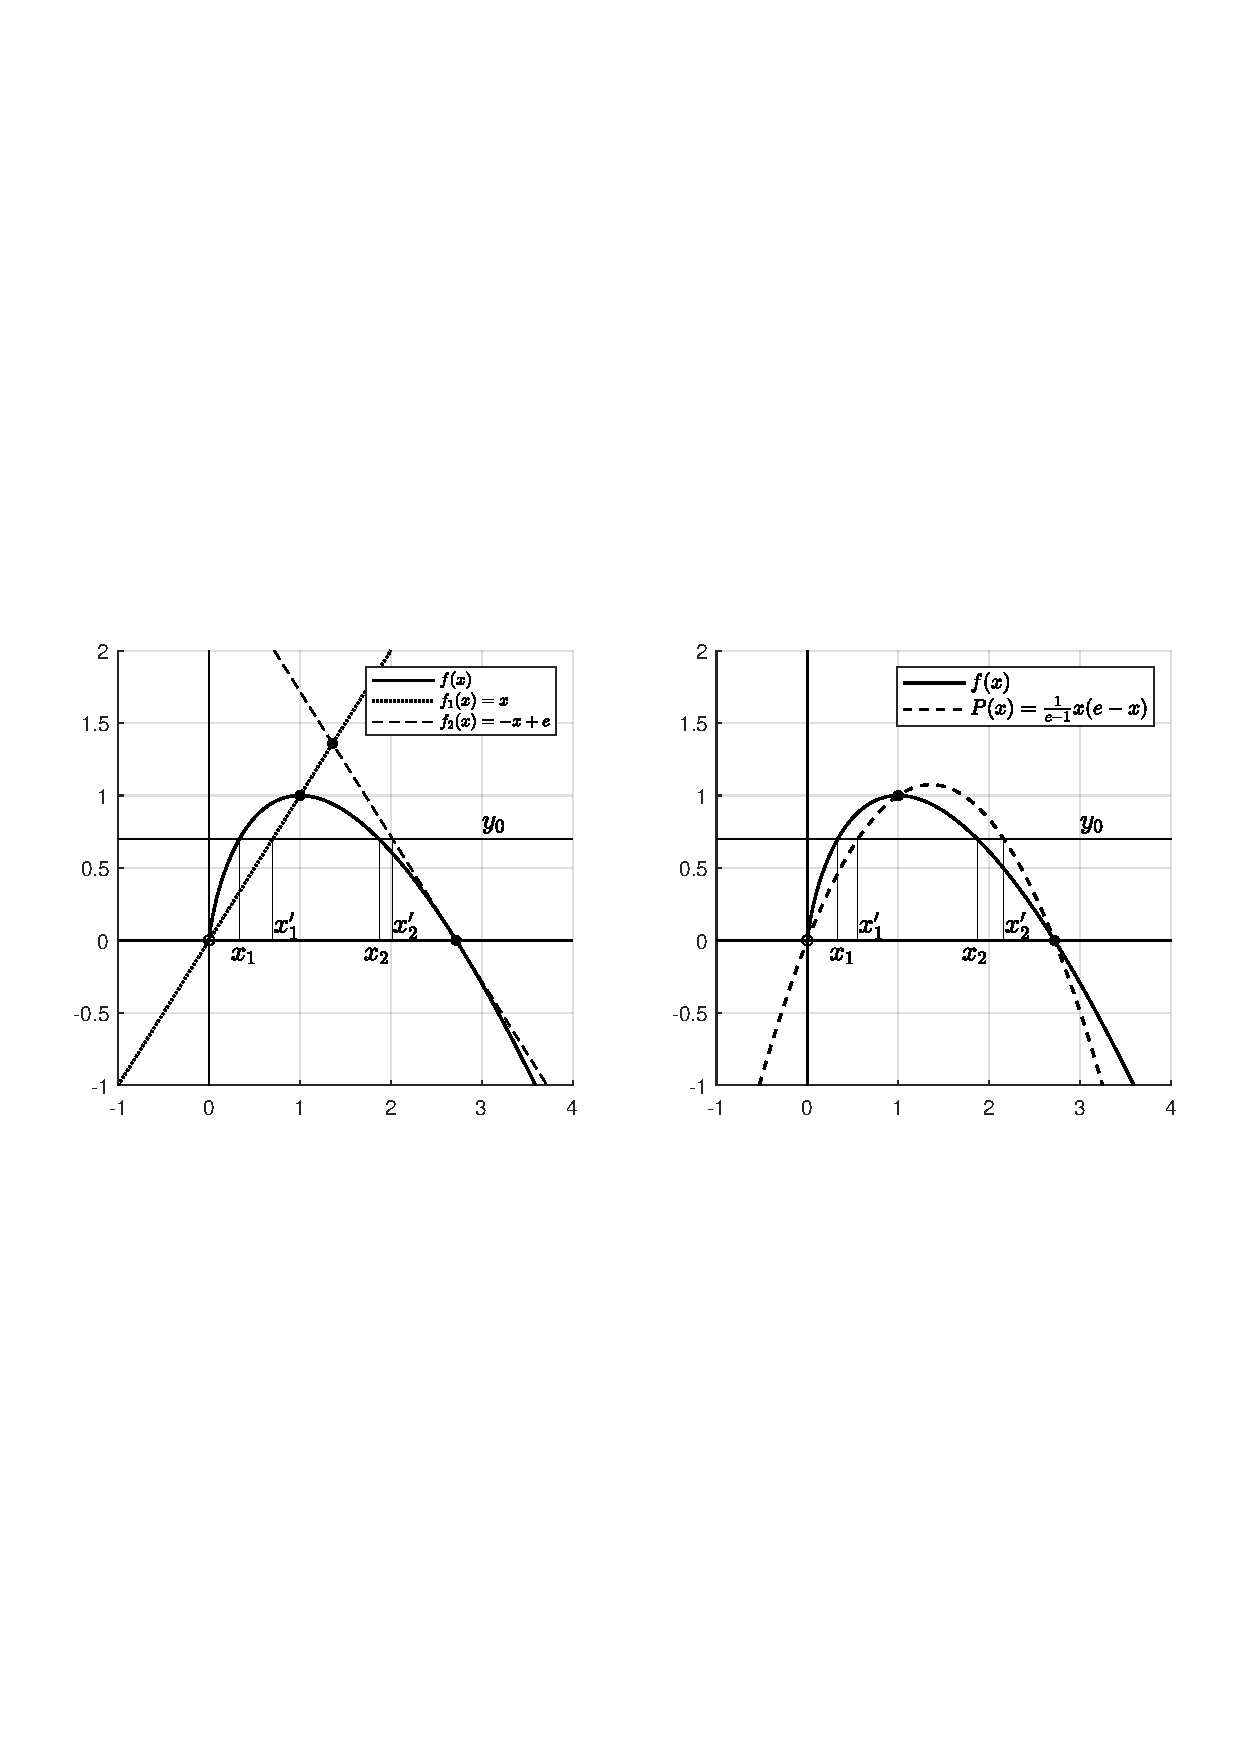
\includegraphics[width=0.9\linewidth]{2021新高考全国I卷图2}
\end{figure}

证明$ x_1+x_2<\e $的\textbf{方法二}:作一条过$ (0,0) $和$ (1,1) $的直线$ y=f_1(x)=x $,这条直线是$ y=f(x) $的割线,再作$ y=f(x) $在$ (\e,0) $处的切线,$ f'(\e)=-1 $,所以切线方程为$ y=f_2(x)=-x+\e $.容易验证,当$ x>0 $时,$ f(x)\leq f_2(x) $,等号仅在$ x=\e $处成立。割线与切线的交点坐标为$ (\dfrac{\e}{2},\dfrac{\e}{2}) $,割线和切线关于直线$ x=\dfrac{\e}{2} $对称。设$ f(x_1)=f_1(x_1')=f(x_2)=f_2(x_2')=y_0\in(0,1) $,那么$ x_1<x_1'=y_0<1<x_2<x_2'=-y_0+\e<\e $,于是$ x_1+x_2<x_1'+x_2'=y_0+(-y_0+\e)=\e $. 

证明$ x_1+x_2<\e $的\textbf{方法三}:使用过原点、零点$ (\e,0) $和极大值点$ (1,1) $
的抛物线$ P(x)=\dfrac{1}{\e-1}x(\e-x) $,容易证明,
当$ x\in(0,1) $时,$ f(x)>P(x) $,
当$ x\in(1,\e) $时,$ f(x)<P(x) $,设$ f(x_1)=P(x_1')=f(x_2)=P(x_2')=y_0\in(0,1) $,那么$ x_1<x_1'<1<x_2<x_2'<\e $,于是$ x_1+x_2<x_1'+x_2'=\e $.
(因为抛物线的对称轴是$ x=\dfrac{\e}{2} $). 

\item (2021,浙江高考) 设$ a,b $为实数,且 $ a>1 $,函数
$ f(x)=a^{x}-bx+\e^{2}\ (x\in\mathbf{R}) $.\\
(I)求函数 $ f(x) $ 的单调区间;\\
(II)若对任意 $ b>2\e^{2} $,函数
$ f(x) $ 有两个不同的零点,求 $ a $ 的取值范围;\\
(III)当 $ a=\e $时,证明:对任意
$ b>\e^{4} $,函数$ f(x) $有两个不同的零点
$ x_{1},x_{2} $,满足$ x_{2}>\dfrac{b\ln b}
{2\e^{2}}x_{1}+\dfrac{\e^{2}}{b} $ . 
(注: $ \e=2.71828\cdots $ 是自然对数的底数。) \\
\textbf{解}\ (I) $ f'(x)=a^x\ln a-b $,若$ b\leq 0 $,则
$ f(x) $在\textbf{R}上单调递增。若$ b>0 $,则$ f'(x) $零点为
$ x_0=\log_a\dfrac{b}{\ln a}=\dfrac{\ln b-\ln(\ln a)}{\ln a} $,$ f(x) $在
$ (-\infty,x_0) $上单调递减,在$ (x_0,+\infty) $上单调递增,
在$ x_0 $处取得极小值。\\
(II) $ \lim\limits_{x\to-\infty}f(x)=+\infty $,
$ \lim\limits_{x\to+\infty}f(x)=+\infty $,结合(I)中的单调性,
只需$ f(x_0)<0 $即可让$ f(x) $有两个零点,
\begin{align}
    f(x_0) & =a^{x_0}-bx_0+\e^2 \nonumber \\
    & =\dfrac{b}{\ln a}-b\cdot \dfrac{\ln b-\ln(\ln a)}{\ln a}+
    \e^2\q (\text{消去}\ x_0) \label{2021浙江(2)消去x0}\\
    & =a^{x_0}-(a^{x_0}\ln a)x_0+\e^2 \q (\text{消去}\ b) \label{2021浙江(2)消去b}
\end{align}
\textbf{方法一}\ 因为$ a>1 $,所以(\ref{2021浙江(2)消去x0})式等价于
\begin{gather}
    b -b\ln b+b\ln(\ln a)+\e^2\ln a<0 \label{2021浙江g(b)<0}
\end{gather}
对任意$ b>2\e^2 $恒成立,将上式左侧定义为$ g(b) $,
则$ g'(b)=-\ln b+\ln(\ln a) $. \\
\mycircled{1} 若$ \ln a>2\e^2 $,则$ g'(\ln a)=0 $,
$ g(b) $在$ b=\ln a $时取得极大值,但$ g(\ln a)=(1+\e^2)\ln a>0 $,
不符合(\ref{2021浙江g(b)<0})式。\\
\mycircled{2} $ \ln a\leq 2\e^2 $,则$ g'(b)<0 $,
$ g(b) $在$ (2\e^2,+\infty) $上单调递减,只需$ g(2\e^2)\leq 0 $
即可满足(\ref{2021浙江g(b)<0})式,
\begin{gather*}
    g(2\e^2)=2\e^2-2\e^2\ln(2\e^2)-2\e^2\ln(\ln a)+\e^2\ln a\leq 0 \\
    -2\ln 2-2+2\ln(\ln a)+\ln a\leq 0 \q \Rightarrow \q
    \ln\left[\dfrac{(\ln a)^2 a}{4\e^2}\right] \leq 0 
\end{gather*}
$ (\ln a)^2 a\leq 4\e^2\ \Rightarrow\ a\leq \e^2 $,
所以,$ a $的范围是$ (1,\e^2] $. \\
\textbf{方法二}\ 从(\ref{2021浙江(2)消去b})式出发,
令$ h(x)=a^{x}-(a^{x}\ln a)x+\e^2\ (x\in \textbf{R}) $,
则$ h'(x)=-xa^x(\ln a)^2 $,$ h(x) $在$ (0,+\infty) $
上单调递减,又有$ x=\log_a \e^2=\dfrac{2}{\ln a} $
作为$ h(x) $的零点,所以
\begin{gather*}
    x_0=\log_a\dfrac{b}{\ln a}> \log_a \e^2\ 
    \Rightarrow\  b>(\ln a)\e^2
\end{gather*}
于是$ (\ln a)\leq 2 $,$ 1<a\leq \e^2 $. \\
\textbf{方法三}\ $ \dfrac{a^x+\e^2}{x}=b $有两个零点,
令$ J(x)=\dfrac{a^x+\e^2}{x} $,
则$ J'(x)=\dfrac{xa^x\ln a-a^x-\e^2}{x^2}=
\dfrac{a^x\ln (a^x)-a^x-\e^2}{x^2} $,
当$ a^x=\e^2 $,即$ x=\dfrac{2}{\ln a} $时,$ J'(x)=0 $,
$ J(x) $取得极小值$ (\ln a)\e^2 $,所以$ (\ln a)\e^2\leq 2\e^2 $,
$ a\leq \e^2 $. \\
(III) $ \dfrac{e^{x_1}+\e^2}{x_1}=\dfrac{e^{x_2}+\e^2}{x_2}=b $,
$ J(x)=\dfrac{e^x+\e^2}{x} $在$ (0,2) $上单调递减,在$ (2,+\infty) $
上单调递增,$ J(2)=\e^2 $为$ J(x) $的极小值。
因为$ J(\ln 2)=\dfrac{2+\e^2}{\ln 2}<\e^4<b $\ 
(注意$ \e^4>7.29^2>7^2=49,\ \ln2\approx 0.6931 $),所以$ 0<x_1<\ln 2<2 $.
\begin{gather*}
    b=\dfrac{\e^{x_1}+\e^2}{x_1}<\dfrac{\e^2+\e^2}{x_1}
    =\dfrac{2\e^2}{x_1}\q \Rightarrow \q x_1<\dfrac{2\e^2}{b}
\end{gather*}

再尝试找出$ x_2 $所大于的最大整数。
$ \dfrac{\e^4+\e^2}{4}<\e^4 $(当然,$ x_2>\ln b>4 $);
$ \dfrac{\e^5+\e^2}{5}<\e^4\ \Leftrightarrow\ 
\e+\dfrac{1}{\e^2}<5 $;
$ \dfrac{\e^6+\e^2}{6}>\dfrac{7.29\e^4+\e^2}{6}>\e^4 $. 
所以$ x_2>5 $,
\begin{gather*}
    b=\dfrac{\e^{x_2}+\e^2}{x_2}<\dfrac{e^{x_2}+\e^2}{5} \q
    \Rightarrow\q x_2>\ln(5b-\e^2)
\end{gather*}

只需证明
\begin{gather}
    \ln(5b-\e^2)>\dfrac{b\ln b}{2\e^{2}}\dfrac{2\e^2}{b}
    +\dfrac{\e^{2}}{b}=\ln b+\dfrac{\e^{2}}{b} \nonumber \\
    \Leftrightarrow\ 
    \ln\left(5-\dfrac{\e^{2}}{b}\right)>\dfrac{\e^{2}}{b}
    \label{2021浙江ln(5-x)>x}
\end{gather}
令$ K(x)=\ln(5-x)-x\ (0<x<5) $,显然$ K(x) $单调递减,
$ K(1)=2\ln 2-1>0 $,所以,当$ x\in(0,1) $时,
$ K(x)>0 $,而$ \dfrac{\e^{2}}{b}<\dfrac{\e^{2}}{\e^4}<1 $,
所以(\ref{2021浙江ln(5-x)>x})式成立。证毕。\\
\textbf{注1}:如果想到利用不等式$ \e^x<\dfrac{2+x}{2-x}\ (0<x<2) $,那么
\begin{gather}
    b=\dfrac{\e^{x_1}+\e^2}{x_1}<\dfrac{\frac{2+x_1}{2-x_1}+\e^2}{x_1}
    \nonumber \\
    bx_1^2+(1-\e^2-2b)x_1+2+2\e^2>0 \nonumber \\
    x_1<\dfrac{(2b+\e^2-1)-\sqrt{(1-\e^2-2b)^2-4b(2+2\e^2)}}{2b} 
    \label{2021浙江x1二次不等式}
\end{gather}
将(\ref{2021浙江x1二次不等式})式右侧关于$ b $的函数记为$ \varphi(b) $,
$ \varphi(b) $表达式过于复杂,手算难以继续。借助用计算机可以验证下式成立
\begin{gather*}
    \ln(5b-\e^2)>\ln b+\dfrac{\e^{2}}{b}
    >\dfrac{b\ln b}{2\e^{2}}\varphi(b)+\dfrac{\e^{2}}{b}
\end{gather*}
三个函数图像如下:
\begin{figure}[!ht] % ZheJiang2021.m
    \centering
    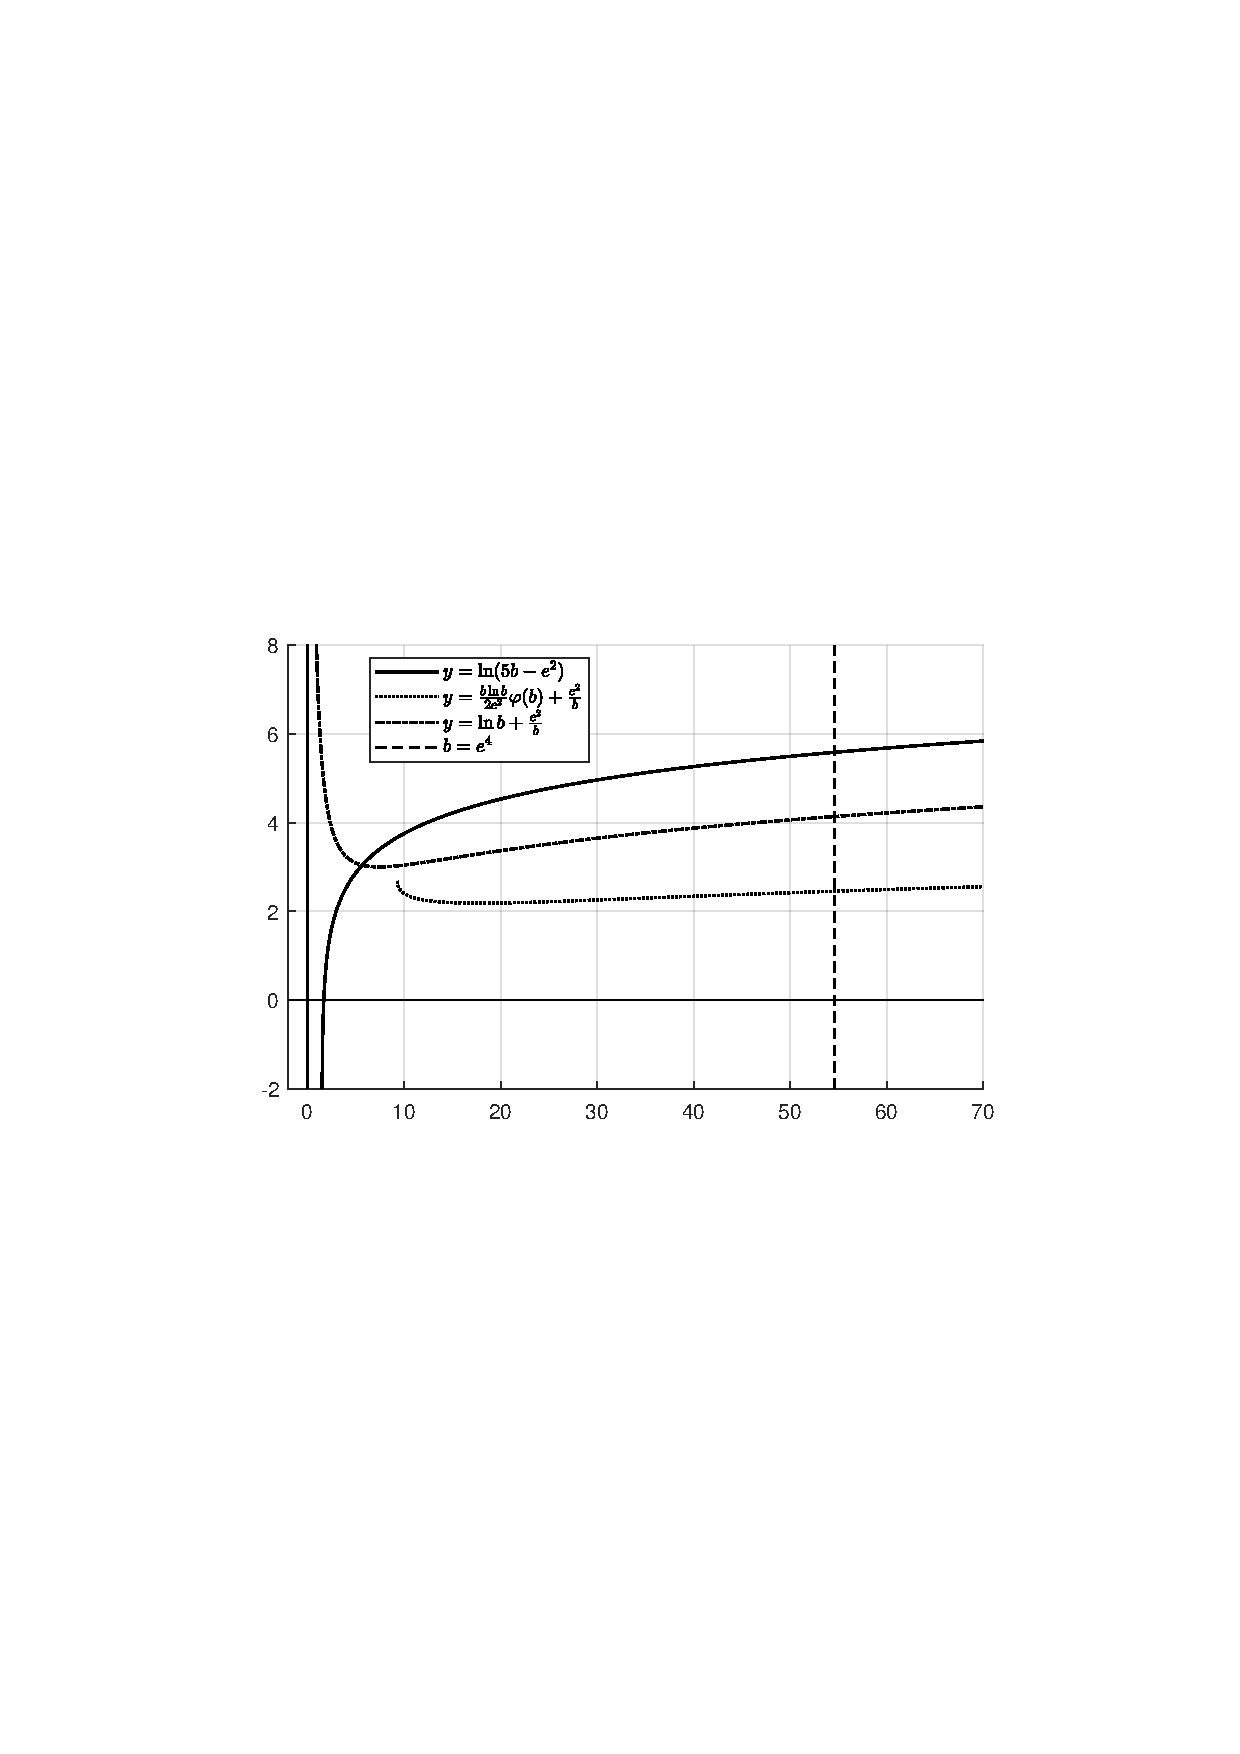
\includegraphics[width=0.7\linewidth]{2021浙江图1}
\end{figure}

可以看出三个函数差距很大,意味着原始不等式可以大大地加强,
感兴趣的读者自行研究。\\
\textbf{注2}:若对$ h(x) $稍作整理,$ h(x)=a^x-a^x\ln(a^x)+\e^2 $,
发现$ a^x $出现3次,可以做代换$ t=a^x>0 $,
令$ \varphi(t)=t-t\ln t+\e^2 $,则$ \varphi'(t)=-\ln t $,
$ \varphi(t) $在$ (1,+\infty) $上单调递减,且
$ \varphi(\e^2)=0 $,所以$ t_0=a^{x_0}=\dfrac{b}{\ln a}>\e^2 $,剩余略。
对于$ J(x) $,也可以做换元$ u=x\ln a $.

巧合的是,这一题与2021年新高考全国I卷一样,都出现了函数$ y= x-x\ln x $. 不知道命题人是有意还是无意,函数$ y= x-x\ln x $可是大有来头:与黎曼猜想有关!黎曼zeta函数的所有非平凡零点(或者说是复数零点)的实部都是$ \dfrac{1}{2} $(尚未证明),
虚部大于0而小于$ T $的复数零点的数量大约为
$ \dfrac{T}{2\pi}\ln\dfrac{T}{2\pi}-\dfrac{T}{2\pi} $(已经证明\footnote{参见Edwards H. M. Riemann's Zeta Function[M]. Academic Press, New York, (1974). 第6.7节 BACKLUND'S ESTIMATE OF $ N(T) $}).
如果设$ y=x\ln x-x $的反函数为$ y=F(x) $(写不出显式表达式),
那么将这些复数零点\footnote{复数零点数据来源 http://www.dtc.umn.edu/\~{}odlyzko/zeta\_{}tables/index.html,前10个虚部的数值为:
\begin{align*}
    & 14.134725142,\ 21.022039639,\ 25.010857580,\ 30.424876126,
    \ 32.935061588,\ 37.586178159,\ 40.918719012, \\
    & 43.327073281,\ 48.005150881,\ 49.773832478,\ 52.970321478,
    \ 56.446247697,\ 59.347044003,\ 60.831778525
\end{align*}
}按虚部从小到大排列时,
第$ N $个虚部的大小大约为$ 2\pi F(N) $. 图像如下:
% RiemannZetaZero.m
\begin{figure}[H]
    \centering
    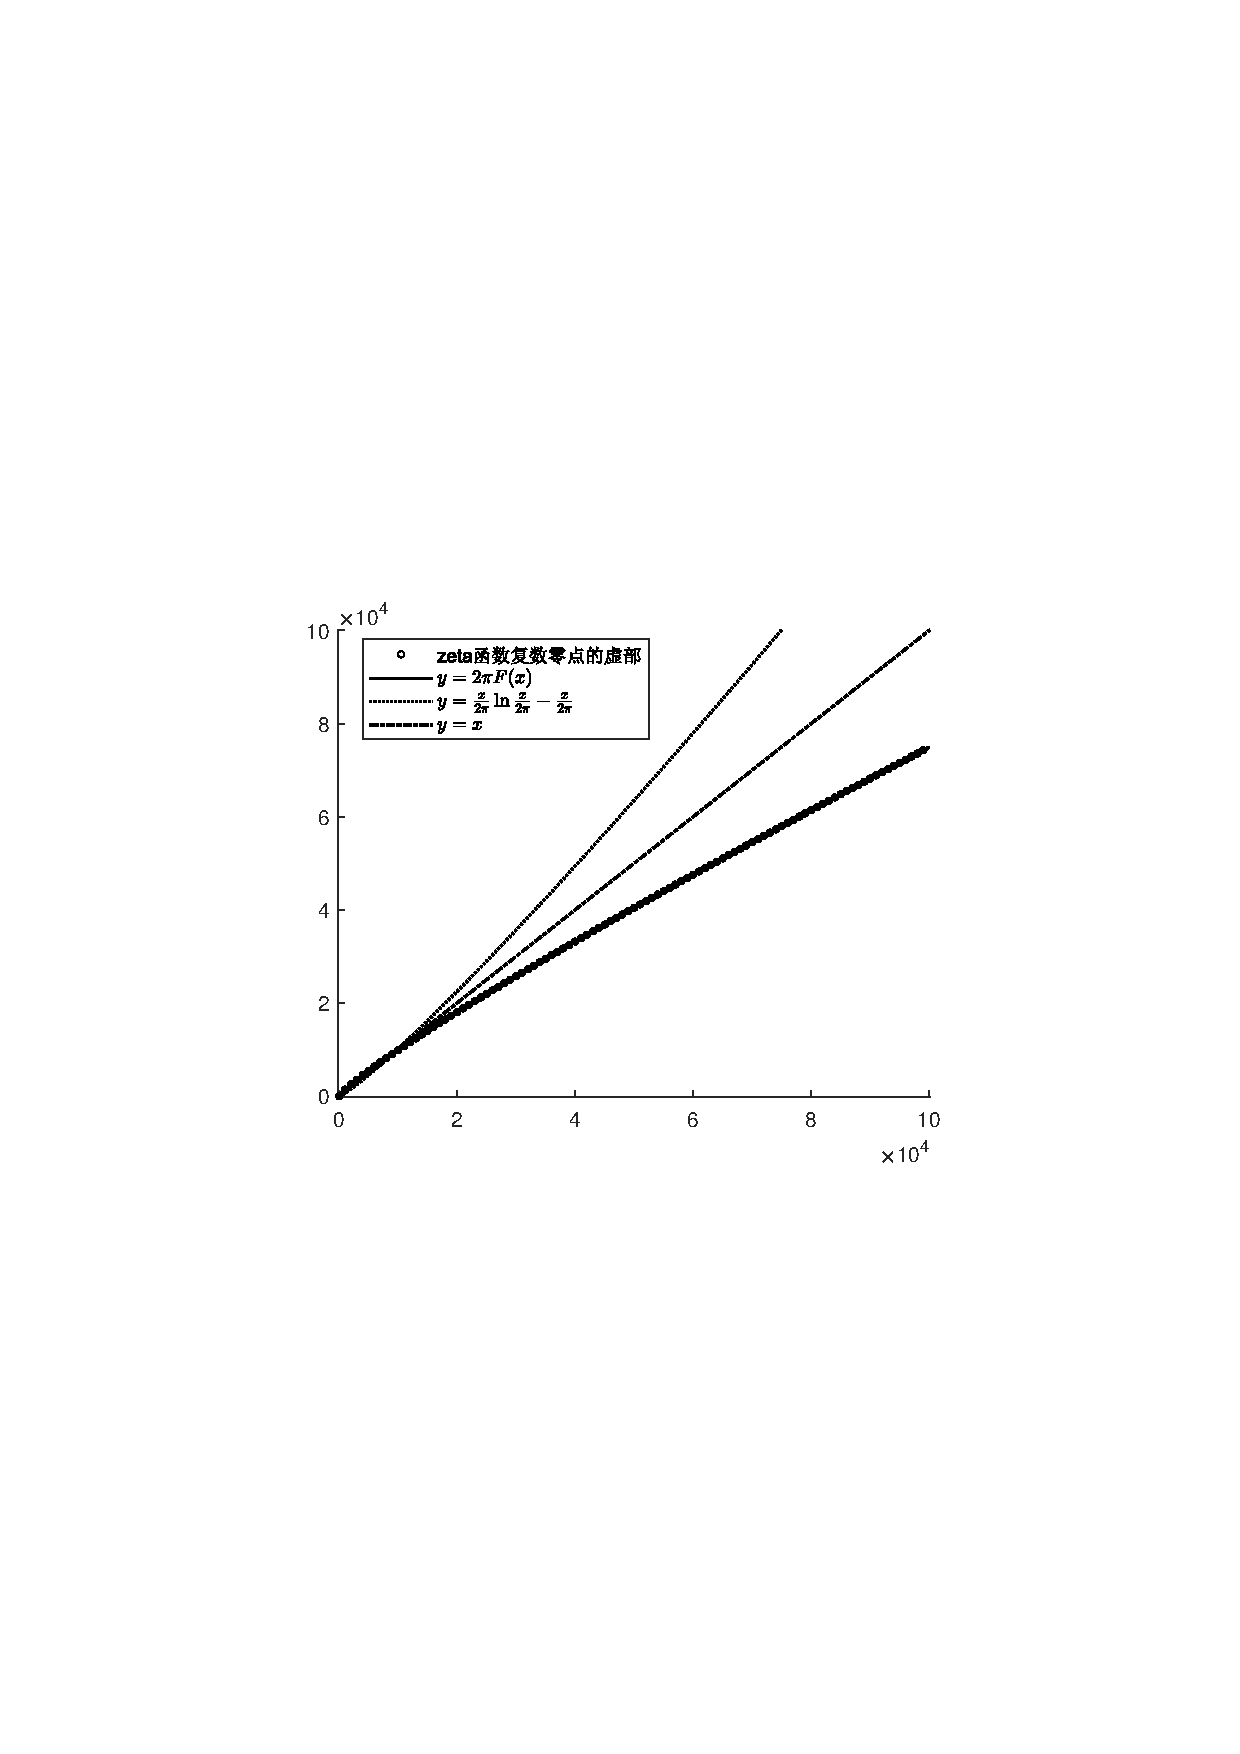
\includegraphics[width=0.6\linewidth]{zeta函数虚部拟合}
\end{figure}

从图中可以看出,用$ y=2\pi F(x) $拟合复数零点的虚部的效果是非常好的。
不过,也只是拟合,而不是精确的通项公式。

% QuanGuo_I_2016.m
\item (2016,全国I卷)已知函数$ f(x)=(x-2)\e^{x}+a(x-1)^2 $有两个零点, \\
(1) 求$ a $的取值范围;\\
(2) 设$ x_1,x_2 $为$ f(x) $的两个零点,证明:$ x_1+x_2<2 $。\\
\textbf{解}\ (1)\textbf{方法一}\ 等价于函数$ g(x)=\dfrac{(x-2)\e^x}{(x-1)^2} $与直线$ y=-a $有两个交点。$ g'(x)=\dfrac{(x-2)^2+1}{(x-1)^3} \e^x $,当$ x\in(-\infty,1) $时,$ g'(x)<0,\ g(x)<0,\ g(x) $单调递减;当$ x\in(1, +\infty) $时,$ g'(x)>0,\ g(x) $单调递增,$ g(x) $有且仅有$ x=2 $一个零点,$ g(x) $图像如下,所以当$ -a<0 $时,$ y=-a $才能与$ y=g(x) $有两个交点,$a>0 $.
\begin{figure}[h]
    \centering
    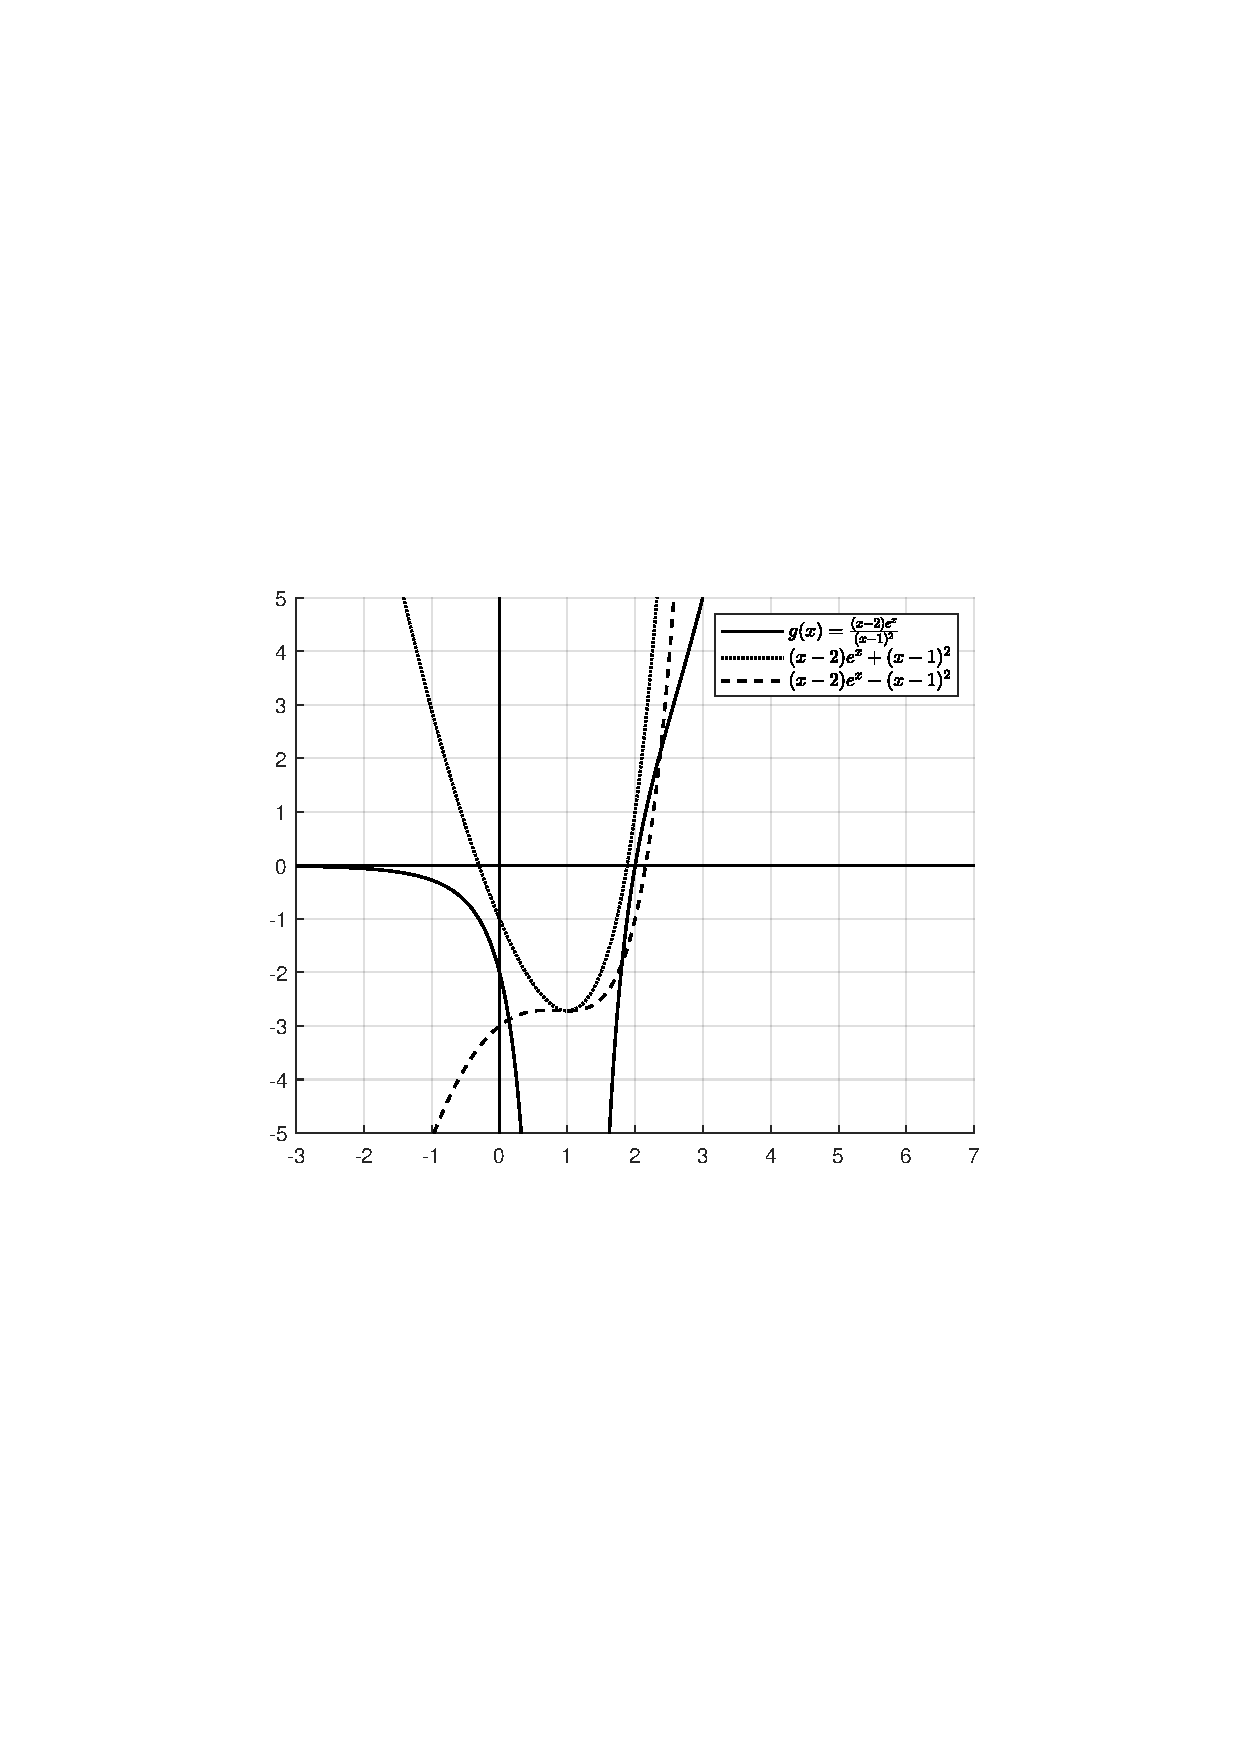
\includegraphics[width=0.5\linewidth]{2016全国I卷}
\end{figure} \\
\textbf{方法二}\ $ f'(x)=(x-1)\e^x+2a(x-1)=(x-1)(\e^x+2a) $.\\
\mycircled{1} 若$ a=0 $,则$ f(x) $有且仅有$ x=2 $一个零点,不符合题意,所以$ a\neq 0 $.\\
\mycircled{2} 若$ a>0 $,则$ f(x) $在$ (-\infty,1) $上单调递减,在$ (1,+\infty) $上单调递增,在$ x=1 $处取得极小值$ -\e<0 $,且$ f(-\infty)=+\infty,\ f(+\infty)=+\infty $,所以$ f(x) $在$ (-\infty,1) $和$ (1,+\infty) $上各有一个零点,符合题意。\\
\mycircled{3} 若$ a<0 $,按$ \e^x+2a=0 $的根与1的相对大小分成两类,\\
(i) $ \ln(-2a)\leq 1 $,那么$ f(x) $在$ (1,+\infty) $上单调递增,同时有$ f(x)<0,\ (x<1) $,所以$ f(x) $有且仅有一个零点,不符合题意。\\
(ii) $ \ln(-2a)> 1 $,$ f(x)<0,\ (x<1) $,$ f(x) $在$ (1,\ln(-2a)) $上单调递减,在$ (\ln(-2a),+\infty) $上单调递增,$ f(1)=-\e<0,\ f(\ln(-2a))=a[(x-2)^2+1]<0 $,所以$ f(x) $有且仅有一个零点(在$ (\ln(-2a),+\infty) $内),不符合题意。\\
综上所述,$ a>0 $. \\
(2) 令$ h(x)=g(x)-g(2-x)=\dfrac{(x-2)\e^x}{(x-1)^2}-\dfrac{(-x)\e^{2-x}}{(x-1)^2}=\dfrac{(x-2)\e^x+x\e^{2-x}}{(x-1)^2} $,再令$ \varphi(x)=(x-2)\e^x+x\e^{2-x} $,则$ \varphi'(x)=(x-1)\e^x+(1-x)\e^{2-x}=(x-1)\dfrac{\e^{2x}-\e^{2}}{\e^x}\geq 0 $,所以$ \varphi(x) $在\textbf{R}上单调递增,当$ x>1 $时,$ \varphi(x)>\varphi(1)=0,\ h(x)>0 $.不妨设$ x_1<1<x_2 $,则$ g(x_1)=g(x_2)=-a $,$ h(x_2)=g(x_2)-g(2-x_2)>0 $,$ g(x_1)=g(x_2)>g(2-x_2) $,$ x_1 $和$ 2-x_2 $
同属于$ g(x) $的单调递减区间$ (-\infty,1) $,所以$ x_1<2-x_2,\ x_1+x_2<2 $. 

\item (2016,天津高考)已知函数$ f(x)=x^3-ax-b,\ x\in \textbf{R},a,b\in 
\textbf{R} $.\\
(1)求$ f(x) $的单调区间;\\
(2)若$ f(x) $存在极值点$ x_0 $,且$ f(x_0)=f(x_1)\ (x_0\neq x_1) $,求证:$ 2x_0+x_1=0 $;\\
(3)设$ a>0 $,求证:$ |f(x)| $在区间$ [-1,1] $上的最大值不小于$ \dfrac{1}{4} $.\\
\textbf{解}\ (1)略。\\
(2)\ $ f'(x)=3x^2-a $,$ f'(x_0)=3x_0^2-a=0 $,由$ f(x_0)=f(x_1) $可得:
\begin{gather*}
    x_0^3-ax_0=x_1^3-ax_1 \\
    x_0^3-x_1^3=(x_0-x_1)(x_0^2+x_0x_1+x_1^2)=a(x_0-x_1)\q (x_0\neq x_1) \\
    x_0^2+x_0x_1+x_1^2=a=3x_0^2 \\
    x_1^2+x_0x_1-2x_0^2=(x_1-x_0)(x_1+2x_0)=0 \\  
    x_1+2x_0=0
\end{gather*}  
(3) 根据前面提到的定理,$ n $次首一多项式在$ [-1,1] $上的绝对值的最大值不小于
$ \dfrac{1}{2^{n-1}} $,本题是三次首一多项式,所以不小于$ \dfrac{1}{4} $. 
严格证明如下:
\begin{align*}
    M&\geq |f(-1)|=|-1+a-b| \\
    M&\geq |f(1)|=|1-a-b|=|-1+a+b| \\
    2M&\geq 2|f(-\dfrac{1}{2})|=2|-\dfrac{1}{8}+\dfrac{1}{2}a-b|=
    |\dfrac{1}{4}-a+2b| \\
    2M&\geq 2|f( \dfrac{1}{2})|=2| \dfrac{1}{8}-\dfrac{1}{2}a-b|=
    |\dfrac{1}{4}-a-2b|	  
\end{align*}
将以上4个式子相加,并利用三角不等式,有
\begin{gather*}
    6M\geq |(-1+a-b)+(-1+a+b)+(\dfrac{1}{4}-a+2b)+(\dfrac{1}{4}-a-2b)|
    =\dfrac{3}{2}
\end{gather*}
所以,$ M\geq \dfrac{1}{4} $.上面4个式子在$ M $前面配的系数,是先设为未知数,再解方程
组得出的。如果不取$ \pm 1,\pm \dfrac{1}{2} $这4个点,比如把$ \pm \dfrac{1}{2} $
换成$ \pm \dfrac{1}{3} $,那么
\begin{align*}
    3M&\geq 3|f(-\dfrac{1}{3})|=3|-\dfrac{1}{27}+\dfrac{1}{3}a-b|=
    |\dfrac{1}{9}-a+3b| \\
    3M&\geq 3|f( \dfrac{1}{3})|=3| \dfrac{1}{27}-\dfrac{1}{3}a-b|=
    |\dfrac{1}{9}-a-3b|  
\end{align*}
同样取4个式子相加,
\begin{align*}
    8M\geq |(-1+a-b)+(-1+a+b)+(\dfrac{1}{9}-a+3b)+(\dfrac{1}{9}-a-3b)|=
    \dfrac{16}{9}
\end{align*}
于是,$ M\geq \dfrac{2}{9} $,这样是无法证明$ M\geq \dfrac{1}{4} $的。
为什么$ \pm \dfrac{1}{2} $具有特殊地位呢?是因为$ \pm \dfrac{1}{2} $恰好是
$ h(x)=x^3-\dfrac{3}{4}x $的两个极值点横坐标,且$ h(\pm\dfrac{1}{2})=\mp 
\dfrac{1}{4} $. $ h(x) $是首一的三次车比雪夫多项式。

第(3)问的常规做法是按极值点横坐标$ \sqrt{\dfrac{a}{3}} $与
$ \dfrac{1}{2} $和1的相对大小分类讨论,即将$ a $分成$ (0,\dfrac{3}{4}),
[\dfrac{3}{4},3),[3,+\infty) $三个区间,过程过于繁琐,不予介绍。

\item (2017,天津高考)设$ a\in \textbf{Z} $,已知定义在\textbf{R}上的函数$ f(x)=2x^4+3x^3
-3x^2-6x+a $在区间$ (1,2) $内有一个零点$ x_0 $,$ g(x) $为$ f(x) $的导函数。\\
(I)求$ g(x) $的单调区间;\\
(II)设$ m\in [1,x_0)\cup(x_0,2] $,定义函数$ h(x)=g(x)(m-x_0)-f(m) $,求证:
$ h(m)h(x_0)<0 $;
(III)求证:存在大于0的常数$ A $,使得对于任意的正整数$ p,q $,且$ \dfrac{p}{q}\in[1,
x_0)\cup(x_0,2] $,满足$ |\dfrac{p}{q}-x_0|\geq \dfrac{1}{Aq^4} $. \\
\textbf{解}\ (1)\ 以下一律使用$ f'(x) $代替$ g(x) $,能让思路更加清晰。
$ f'(x)=8x^3+9x^2-6x-6 $,$ f''(x)=6(4x^2+3x-1)=6(4x-1)(x+1) $,
所以$ f'(x) $在$ (-\infty,-1) $和$ (\dfrac{1}{4},+\infty) $上分别单调递增,
在$ (-1,\dfrac{1}{4}) $上单调递减。\\
(2)\ 当$ x\geq 1 $时,$ f'(x)\geq f'(1)=5>0 $,所以$ f(x) $在
$ [1,+\infty) $上单调递增,
\begin{align*}
    h(m)  &=f'(m)(m-x_0)-f(m) \\
    h(x_0)&=f'(x_0)(m-x_0)-f(m) 
\end{align*}
令
\begin{align*}
    \varphi_1(t) &=f'(t)(t-x_0)-f(t) \\
    \varphi_2(t) &=f'(x_0)(t-x_0)-f(t) 
\end{align*}
则
\begin{align*}
    \varphi_1'(t) &=f''(t)(t-x_0) \\
    \varphi_2'(t) &=f'(x_0)-f'(t) 
\end{align*}
若$ t\in[1,x_0) $,则$ \varphi_1'(t)<0 $,$ \varphi_1(t)>\varphi_1(x_0)=0 $,
$ \varphi_2'(t)>0 $,$ \varphi_2(t)<\varphi_2(x_0)=0 $,于是$ h(m)h(x_0)<0 $
成立。对于$ t\in(x_0,2] $,论证过程是类似的,结论同样成立。\\
(3) $ h'(x)=f''(x)(m-x_0) $,由(2)可知,当$ m\in[1,x_0),\ x\geq 1 $时,
$ h'(x)<0 $,$ h(x) $仅在区间$ (m,x_0) $内有一个实根;
当$ m\in(x_0,2],\ x\geq 1 $时,$ h'(x)>0 $,$ h(x) $仅在区间$ (x_0,m) $
内有一个实根。将$ h(x) $在区间$ (1,2) $内的唯一零点记为$ x_1 $,则
$ h(x_1)=f'(x_1)\Big(\dfrac{p}{q}-x_0\Big)-f\Big(\dfrac{p}{q}\Big)=0 $.
易知,$ 0<f'(1)<f'(x_1)<f'(2) $,于是
\begin{gather*}
    \left|\frac{p}{q}-x_0\right|=\frac{\left|f\Big(\dfrac{p}{q}\Big)
        \right|}{f'(x_1)}>\frac{\left|f\Big(\dfrac{p}{q}\Big)\right|}{f'(2)}
    =\frac{\left|2p^4+3p^3q-3p^2q^2-6pq^3+aq^4\right|}{f'(2)q^4}
\end{gather*}
因为$ \dfrac{p}{q}-x_0\neq 0 $,所以$ |2p^4+3p^3q-3p^2q^2-
6pq^3+aq^4|>0 $,又因为$ p,q $为正整数,所以
$ |2p^4+3p^3q-3p^2q^2-6pq^3+aq^4| $也是正整数,
那么它必然大于等于1,
\begin{gather*}
    \left|\frac{p}{q}-x_0\right|>\frac{1}{f'(2)q^4}
\end{gather*}
只需令$ A=|f'(2)| $,就有$ \left|\dfrac{p}{q}-x_0\right|>\dfrac{1}{Aq^4} $.\\
\textbf{注}:第(2)问实际上是拉格朗日中值定理,设$ m\in[1,x_0) $,做逆向分析,
有$ h(m)=\varphi_1(m)>0 $,$ h(x_0)=\varphi_2(m)<0 $,$ f'(x_0)(m-x_0)<f(m)
<f'(m)(m-x_0) $,即
\begin{gather}
    f'(x_0)<\frac{f(m)-f(x_0)}{m-x_0}=f'(\xi)<f'(m)
\end{gather}
因为$ f'(x) $在$ (\dfrac{1}{4},+\infty) $上单调递增,所以上式显然成立。

第(3)问实际上是刘维尔逼近定理。

% TianJin2018.m
\item (2018,天津高考)已知函数$ f(x)=a^x,\ g(x)=\log_{a} x $,其中$ a>1 $。\\
(I)求函数$ h(x)=f(x)-x\ln a $的单调区间;\\
(II)若曲线$ y=f(x) $在点$ (x_1,f(x_1)) $处的切线与曲线$ y=g(x) $在点
$ (x_2,g(x_2)) $处的切线平行,证明:$ x_1+g(x_2)=
-\dfrac{2\ln\ln a}{\ln a} $;\\
(III)证明:当$ a\geq \e^{1/\e} $时,存在直线$ l $,使$ l $是曲线
$ y=f(x) $的切线,也是曲线$ y=g(x) $的切线。\\
\textbf{解}\ (I) $ h'(x)=(a^x-1)\ln a $,
$ h(x) $在$ (-\infty,0) $上单调递减,在$ (0,+\infty) $上单调递增。\\
(II) $ f'(x_1)=a^{x_1}\ln a=g'(x_2)=\dfrac{1}{x_2\ln a}\
\Rightarrow \  a^{x_1}x_2=(\ln a)^{-2} $,两边取自然对数
\begin{gather*}
    x_1\ln a+\ln x_2=-2\ln\ln a\q \Rightarrow \q 
    x_1+\frac{\ln x_2}{\ln a}=-\dfrac{2\ln\ln a}{\ln a}
\end{gather*}
(III) 因为$ l $是公切线,所以
\begin{align*}
    f'(x_1) &=g'(x_2)=\dfrac{g(x_2)-f(x_1)}{x_2-x_1} \\
    a^{x_1}\ln a &=\dfrac{1}{x_2\ln a}=\dfrac{\frac{\ln x_2}{\ln a}
        -a^{x_1}}{x_2-x_1}
\end{align*}
\textbf{方法一}\ 消去$ x_2 $,将$ x_2=\dfrac{1}{a^{x_1}(\ln a)^2} $
和$ \ln x_2=-2\ln\ln a-x_1\ln a $代入
\begin{gather*}
    a^{x_1}\ln a =\dfrac{\frac{\ln x_2}{\ln a}-a^{x_1}}{x_2-x_1}
\end{gather*}
可得:
\begin{gather*}
    -x_1a^{x_1}(\ln a)^2+a^{x_1}\ln a +x_1\ln a+2\ln\ln a+1=0
\end{gather*}
只需证明当$ a\geq \e^{1/\e} $时,以上方程存在实数解。

令$ F(x)=-xa^{x}(\ln a)^2+a^{x}\ln a +x\ln a+2\ln\ln a+1\ (x\in \textbf{R}) $,则
\begin{align*}
    F'(x)  &=[1-xa^x(\ln a)^2]\ln a    \\
    F''(x) &=-(1+x\ln a)a^x(\ln a)^3
\end{align*}
$ F''\left(-\dfrac{1}{\ln a}\right)=0 $,
$ F'(x) $在$ \left(-\infty,-\dfrac{1}{\ln a}\right) $上单调递增,
且在$ (-\infty,0) $上恒正,
在$ \left(-\dfrac{1}{\ln a},+\infty\right) $上单调递减。
$ F'(0)=\ln a>0 $,$ F'\left(\dfrac{1}{(\ln a)^2}\right)=
\left[1-a^{1/(\ln a)^2}\right]\ln a<0 $,所以,存在唯一的
$ x_0\in(0,+\infty) $,使得$ F'(x_0)=0 $,即
$ 1-x_0a^{x_0}(\ln a)^2=0 $. 那么$ F(x) $在$ (-\infty,x_0) $上单调递增,在$ (x_0,+\infty) $上单调递减,在$ x=x_0 $处取得极大值。

又因为$ a\geq \e^{1/\e} $,所以$ \ln\ln a\geq -1 $,
\begin{align*}
    F(x_0) &=a^{x_0}\ln a +x_0\ln a+2\ln\ln a-
    \underbrace{x_0a^{x_0}(\ln a)^2}_{=1}+1 \\
    &=a^{x_0}\ln a +x_0\ln a+2\ln\ln a \\
    &\geq 2\sqrt{a^{x_0}\ln a \cdot x_0\ln a} +2\ln\ln a
    =2+2\ln\ln a\geq 0
\end{align*}

当$ x $充分大时,$ F(x) $中的$ -xa^{x}(\ln a)^2 $的绝对值将远大于
$ F(x) $的其它项,所以必有$ F(x)<0 $. 稍微严格一些的证明如下:
由(I)知:$ a^x\geq 1+(\ln a)x $,当$ x>\dfrac{1}{\ln a} $时,
\begin{align*}
    F(x) &=a^{x}\ln a -xa^{x}(\ln a)^2+x\ln a+2\ln\ln a+1 \\
    &=a^{x}(1-x\ln a)\ln a+x\ln a+2\ln\ln a+1  \\
    &\leq(1+x\ln a)(1-x\ln a)\ln a+x\ln a+2\ln\ln a+1  \\
    &=-(\ln a)^3x^2+\ln a+x\ln a+2\ln\ln a+1
\end{align*}
最后一式为开口向下的抛物线,所以必存在实数$ t>\dfrac{1}{\ln a} $,
使得$ u(t)<0 $.

综上所述,当$ a\geq \e^{1/\e} $时,$ F(x)=0 $有实根,
$ y=f(x) $与$ y=g(x) $存在公切线。\\
\textbf{方法二}\ 消去$ x_1 $,将$ x_1=-\dfrac{2\ln\ln a}{\ln a}-
\dfrac{\ln x_2}{\ln a} $和$ a^{x_1}=\dfrac{1}{x_2(\ln a)^2} $代入
\begin{gather*}
    \frac{1}{x_2\ln a}=\dfrac{\frac{\ln x_2}{\ln a}-a^{x_1}}{x_2-x_1}
\end{gather*}
可得:
\begin{gather*}
    -x_2\ln x_2\ln a+\ln x_2 +x_2\ln a+2\ln\ln a+1=0
\end{gather*}
只需证明当$ a\geq \e^{1/\e} $时,以上方程存在实数解。

令$ G(x)=-x\ln x\ln a+\ln x +x\ln a+2\ln\ln a+1\ (x>0) $,则
\begin{align*}
    G'(x)&=\dfrac{1}{x}-\ln x\ln a \\
    G''(x)&=-\dfrac{1}{x^2}-\dfrac{\ln a}{x}=-\dfrac{1+x\ln a}{x^2}<0
\end{align*}
$ G'(x) $在$ (0,+\infty) $上单调递减,$ \lim\limits_{x\to 0}G'(x)= +\infty $,
$ \lim\limits_{x\to +\infty}G'(x)= -\infty $,所以存在唯一的正实数$ s $,使得
$ G'(s)=0 $,即$ s\ln s=\dfrac{1}{\ln a}\in(0,\e] $,且$ s\in (1,e] $,
$ G(x) $在$ x=s $处取得极大值。
\begin{align*}
    G(s)&=-s\ln s\ln a+\ln s +s\ln a+2\ln\ln a+1 \\
    &\geq -1+\sqrt{(\ln s)\cdot (s\ln a)}+2\ln\ln a+1=2+2\ln\ln a\geq 0
\end{align*}
当$ x $充分大时,$ G(x) $中的$ -x\ln x\ln a $的绝对值将远大于
$ G(x) $的其它项,所以必有$ G(x)<0 $. 严格证明如下:
\begin{align*}
    G(x) &= -x\ln x\ln a+\ln x +x\ln a+2\ln\ln a+1 \\
    &=\left(-\frac{1}{2}x\ln x\ln a+\ln x\right)+
    \left(-\frac{1}{2}x\ln x\ln a+x\ln a\right)+(2\ln\ln a+1) \\
    &=\left(1-\frac{1}{2}x\ln a\right)\ln x+
    \left(1-\frac{1}{2}\ln x\right)x\ln a+(2\ln\ln a+1) 
\end{align*}
当以下三个条件满足时,必有$ G(x)<0 $,
\begin{gather*}
    \begin{cases}
        1-\dfrac{1}{2}x\ln a < -1 \\
        1-\dfrac{1}{2}\ln x <0 \\
        \ln x>2\ln\ln a+1
    \end{cases} \Rightarrow 
    \begin{cases}
        x> \dfrac{4}{\ln a} \\
        x>\e^2 \\
        x>(\ln a)^2\e
    \end{cases}
\end{gather*}
剩余略。\\
\textbf{注}:第(III)问的背景是:当曲线$ y=a^x $与$ y=\log_a x $
(两者互为反函数)相切时,切点必在直线$ y=x $上,而且两者均以直线
$ y=x $为切线,设切点为$ (x_0,x_0) $,那么
\begin{align*}
    \begin{cases}
        a^{x_0}=\dfrac{\ln x_0}{\ln a}=x_0 \\
        a^{x_0}\ln a=\dfrac{1}{x_0\ln a}=1
    \end{cases}
\end{align*}
解得,$ x_0=\e,\ a=\e^{1/\e} $. 当$ a>\e^{1/\e} $时,
曲线$ y=a^x $与$ y=\log_a x $没有交点,必能做出两条关于直线
$ y=x $对称的公切线。图像如下:
\begin{figure}[H]
    \centering
    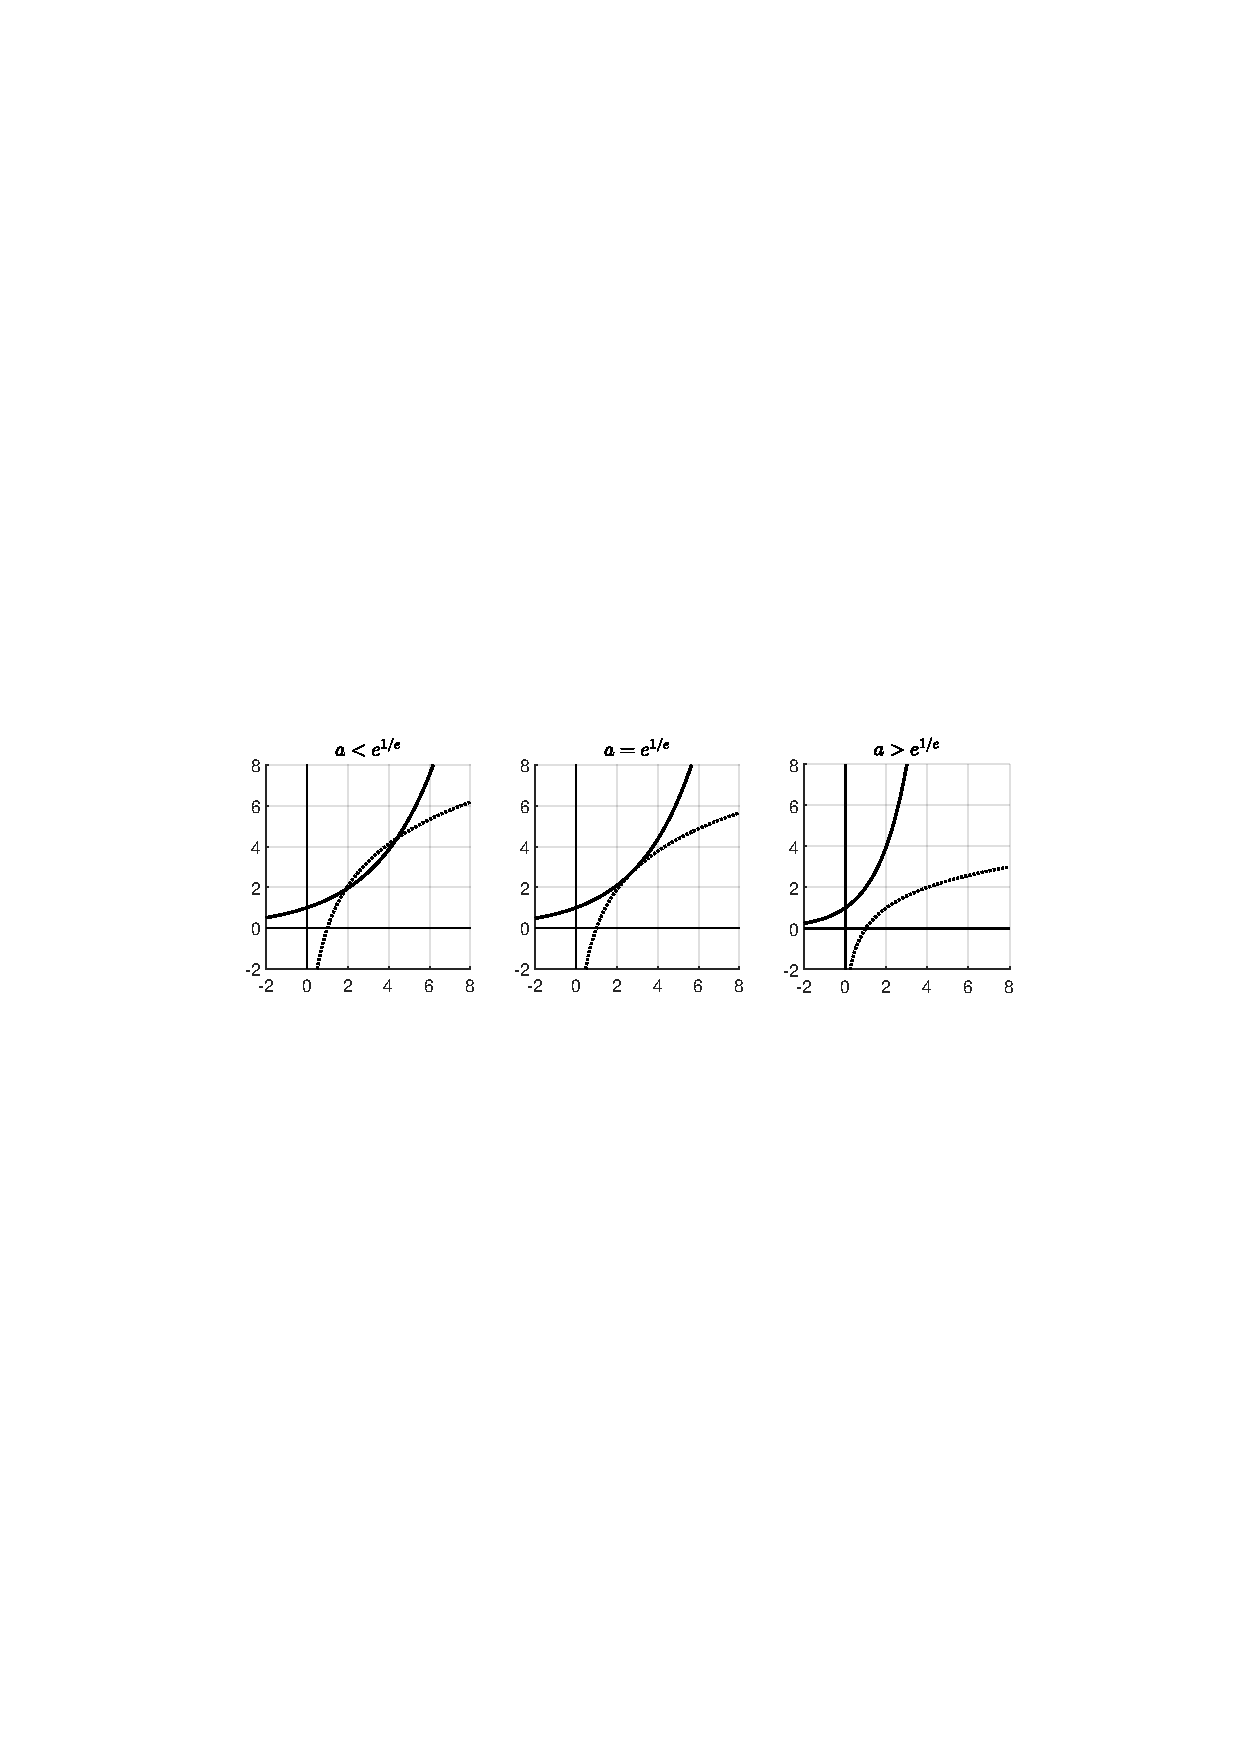
\includegraphics[width=0.9\linewidth]{2018天津高考}
\end{figure}

\item (2019,天津高考,理)设函数$ f(x)=\e^x\cos x $,$ g(x) $为$ f(x) $的导函数。\\
(I)求$ f(x) $的单调区间;\\
(II)当$ x\in \left[\dfrac{\pi}{4},\dfrac{\pi}{2}\right] $时,证明$ f(x)+g(x)\left(\dfrac{\pi}{2}-x\right)\geq 0 $;\\
(III)设$ x_n $为函数$ u(x)=f(x)-1 $在区间$ \left(2n\pi+\dfrac{\pi}{4},2n\pi+
\dfrac{\pi}{2}\right) $内的零点,其中$ n\in \textbf{N} $,证明:
$ 2n\pi+\dfrac{\pi}{2}-x_n<\dfrac{\e^{-2n\pi}}{\sin x_0-\cos x_0} $.\\
\textbf{解}\ (I) $ f'(x)=g(x)=\e^x(\cos x-\sin x)=\sqrt{2}\e^x\cos\left(
x+\dfrac{\pi}{4}\right) $,所以,单调递增区间是 \\
$ \left(2k\pi-\dfrac{3\pi}{4},2k\pi+\dfrac{\pi}{4}\right) $,
单调递减区间是
$ \left(2k\pi+\dfrac{\pi}{4},2k\pi+\dfrac{5\pi}{4}\right) $,
其中$ k\in \textbf{Z} $. \\
(II) 令$ h(x)=f(x)+f'(x)\left(\dfrac{\pi}{2}-x\right) $,则
\begin{gather*}
    h'(x)= f'(x)+f''(x)\left(\dfrac{\pi}{2}-x\right)-f'(x)=
    f''(x)\left(\dfrac{\pi}{2}-x\right)
    =-2\e^x\sin x \left(\dfrac{\pi}{2}-x\right)<0
\end{gather*}
所以,$ h(x)\geq h\left(\dfrac{\pi}{2}\right)=0 $. \\
(III)  $ u(x_{n})=f(x_{n})-1=0 $,即
$ \e^{x_{n}}\cos x_{n}=1 $. 记$ y_{n}=x_{n}-2n\pi $ ,则
$ y_{n}\in\left(\dfrac{\pi}{4},\dfrac{\pi}{2}\right) $ ,
\begin{gather*}
    f(y_{n})=\e^{y_{n}}\cos y_{n}=\e^{x_{n}-2n\pi}
    \cos\left(x_{n}-2n\pi\right)=\e^{-2n\pi},\q (n\in \textbf{N})
\end{gather*}
由$ f(y_{n})=\e^{-2n\pi}\leqslant 1=f(y_{0}) $以及(I)中的
单调递减区间可得:$ y_{n}\geqslant y_{0} $.
由(II)知,当 $ x\in\left[\dfrac{\pi}{4},\dfrac{\pi}{2}\right] $时,$ f''(x)=-2\e^x\sin x<0 $,$ f'(x) $ 在 $ \left[\dfrac{\pi}{4},\dfrac{\pi}{2}\right] $上为减函数,
因此,$ f'(y_{n})\leqslant  f'(y_{0})<f'\left(\dfrac{\pi}{4}\right)=0 $ .
又由(II)知 $ f(y_{n})+f'(y_{n})\left(\dfrac{\pi}{2}-y_{n}\right)\geqslant 0 $,故:
\begin{align*}
    \dfrac{\pi}{2}-y_{n}\leqslant-\dfrac{f\left(y_{n}\right)}{f'\left(y_{n}\right)}=-\dfrac{\e^{-2n\pi}}{f'\left(y_{n}\right)}\leqslant-\dfrac{\e^{-2n\pi}}{f'\left(y_{0}\right)}=\dfrac{\e^{-2n\pi}}{\e^{y_{0}}\left(\sin y_{0}-\cos y_{0}\right)}<\dfrac{\e^{-2n\pi}}{\sin x_{0}-\cos x_{0}}
\end{align*}
所以 $ 2n\pi+\dfrac{\pi}{2}-x_{n}<\dfrac{\e^{-2n\pi}}{\sin x_{0}-\cos x_{0}} $.证毕。 \\
\textbf{注}:如果第(II)问把$ h(x) $中的$ \e^x $约去,改为研究
$ H(x)=\cos x+(\cos x-\sin x)\left(\dfrac{\pi}{2}-x\right) $的正负与单调性,
反倒更麻烦。

因为$ f\left(\dfrac{\pi}{2}\right)=0 $,所以(II)中的不等式可以变形为
\begin{gather*}
    \dfrac{-f(x)}{\frac{\pi}{2}-x}=
    \underbrace{\dfrac{f\left(\frac{\pi}{2}\right)-f(x)}{\frac{\pi}{2}-x}}
    _{\text{割线斜率}}< \underbrace{f'(x)}_{\text{切线斜率}}
    \q \left(\frac{\pi}{4}\leq x<\frac{\pi}{2}\right)
\end{gather*}
请读者结合图形思考上式的含义。

\item $^*$ 对方程$ x=\tan x $的正根作简单介绍,设该方程在区间$ \left(n\pi,
\left(n+\dfrac{1}{2}\right)\pi\right) $上的根为$ x_n\ (n\in
\textbf{N}^+) $,那么\footnote{参见:\\
    $\diamond$ https://mathworld.wolfram.com/TancFunction.html \\
    $\diamond$ https://math.stackexchange.com/questions/110256 \\
    $\diamond$ https://math.stackexchange.com/questions/850992 }:\\
(I) $ \sum\limits_{n=1}^{\infty}\dfrac{1}{x_n^2}=
\dfrac{1}{10} $. \\
(II) 令$ q_n=\left(n+\dfrac{1}{2}\right)\pi $,则
$ x_n $具有如下渐近公式:
\begin{gather*}
    x_n=q_n-\dfrac{1}{q_n}-\dfrac{2}{3q_n^3}-\dfrac{13}{15q_n^5}
    -\dfrac{146}{105q_n^7}-\dfrac{781}{315q_n^9}
    -\dfrac{16328}{3465q_n^{11}}-\cdots
\end{gather*} 
对于(I),可作如下初步分析:
\begin{align*}
    &\sum_{n=1}^{\infty}\dfrac{1}{x_n^2}<\dfrac{1}{\pi^2}
    \sum_{n=1}^{\infty}\dfrac{1}{n^2} =\dfrac{1}{6} \\
    &\begin{aligned}
        \sum_{n=1}^{\infty}\dfrac{1}{x_n^2}> \dfrac{1}{\pi^2}
        \sum_{n=1}^{\infty}\dfrac{1}{\left(n+\frac{1}{2}\right)^2}
        &=\dfrac{4}{\pi^2}\sum_{n=1}^{\infty}\dfrac{1}{(2n+1)^2} \\
        &=\dfrac{4}{\pi^2}\left(\dfrac{\pi^2}{8}-1\right)=
        \dfrac{1}{2}-\dfrac{4}{\pi^2}=0.094715\cdots
    \end{aligned}
\end{align*}
注意:
\begin{align*}
    \sum_{n=1}^{\infty}\dfrac{1}{n^2} &=\dfrac{\pi^2}{6},\qquad 
    \sum_{n=1}^{\infty}\dfrac{1}{(2n)^2} =
    \dfrac{1}{4}\cdot\dfrac{\pi^2}{6}=\dfrac{\pi^2}{24} \\
    \sum_{n=0}^{\infty}\dfrac{1}{(2n+1)^2} &=
    \sum_{n=1}^{\infty}\dfrac{1}{n^2}-\sum_{n=1}^{\infty}\dfrac{1}{(2n)^2}=
    \dfrac{\pi^2}{6}-\dfrac{\pi^2}{24}=\dfrac{\pi^2}{8} 
\end{align*}
对于(II)中的公式,则涉及到拉格朗日反演。

\item (2019,天津高考,文)设函数$ f(x)=\ln x-a(x-1)\e^x $,其中$ a\in \textbf{R} $. \\
(I) 若$ a\leq 0 $,讨论$ f(x) $的单调性;\\
(II) 若$ 0<a<\dfrac{1}{\e} $, 

(i) 证明:$ f(x) $恰有两个零点;

(ii) 设$ x_0 $为$ f(x) $的极值点,$ x_1 $为$ f(x) $的零点,且$ x_1>x_0 $,证明:$ 3x_0-x_1>2 $. \\
\textbf{解}\ (I)$ f'(x)=\dfrac{1}{x}-ax\e^x $,余下省略。
\begin{figure}[h]
	\centering
	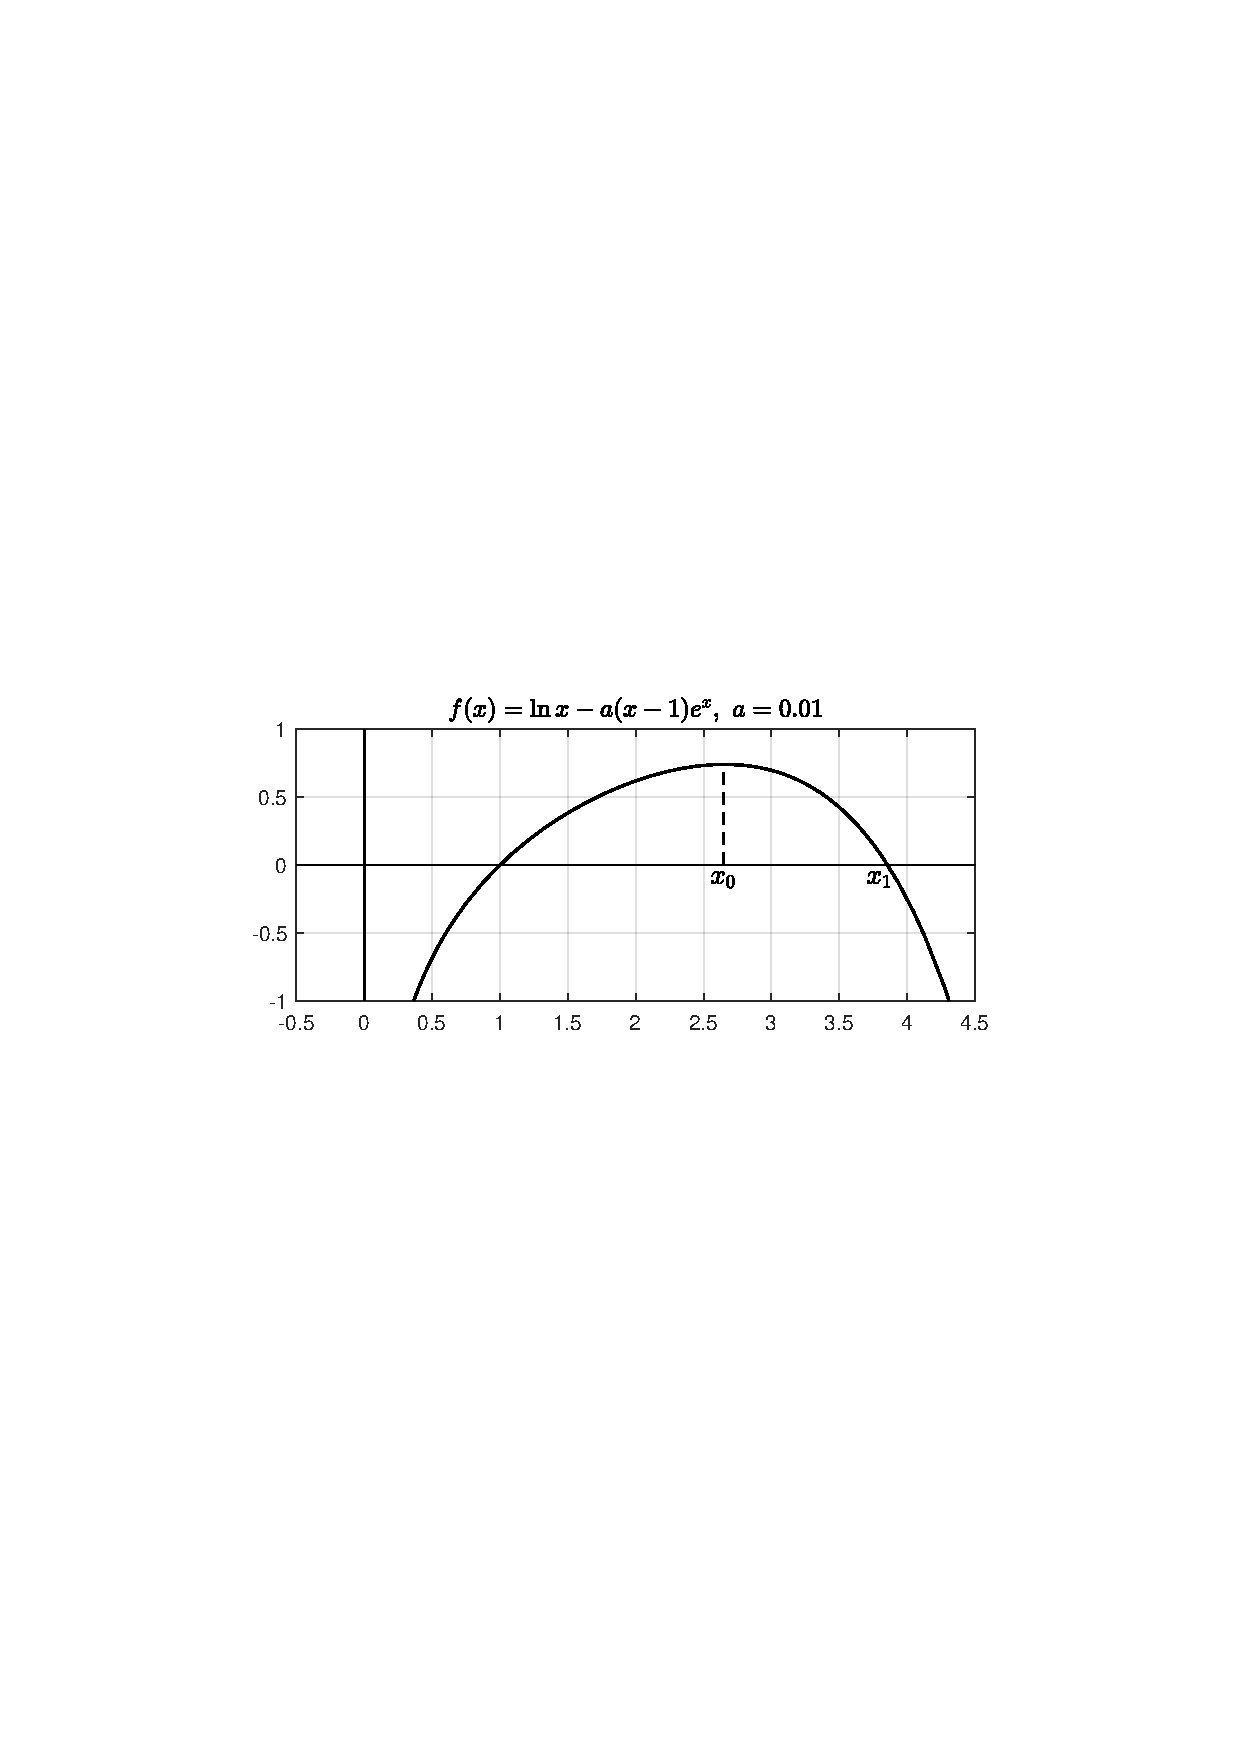
\includegraphics[width=0.5\linewidth]{2019天津高考文科}
\end{figure} \\
(II) (i) $ x=1 $是一个显然的零点,$ f'(x_0)=\dfrac{1}{x_0}-ax_0\e^{x_0}=0,\ x_0^2\e^{x_0}=\dfrac{1}{a}>\e=1^2 \e^1 $,因为函数$ x^2\e^x $在$ (0,+\infty) $上单调递增,所以$ x_0>1 $. 而$ f(x_0)=\ln x_0-a(x_0-1)\e^{x_0}=\ln x_0-a(x_0-1)\cdot \dfrac{1}{ax_0^2}=\ln x_0-\dfrac{1}{x_0}+\dfrac{1}{x_0^2} $,令$ g(x)=\ln x-\dfrac{1}{x}+\dfrac{1}{x^2}\ (x\geq 1) $,则$ g'(x)=\dfrac{(x+2)(x-1)}{x^3}\geq 0 $,所以$ g(x) $在$ (1,+\infty) $上单调递增,$ f(x_0)=g(x_0)>g(1)=0 $. 因为$ f(x) $在$ (0,x_0) $上单调递增,在$ (x_0,+\infty) $上单调递减,且$ f(x_0)>0,\ \lim\limits_{x\to 0}f(x)=-\infty,\ \lim\limits_{x\to +\infty}f(x)=-\infty $,由零点存在定理,$ (x_0,+\infty) $内必有一个零点,所以$ f(x) $恰有两个零点。

(ii)\ $ 1<x_0<x_1,\ a=\dfrac{1}{x_0^2\e^{x_0}}=
\dfrac{\ln x_1}{(x_1-1)\e^{x_1}} $.另外,$ 0<\ln x_1<x_1-1,\ 0<\dfrac{\ln x_1}{x_1-1}<1 $,所以,
\begin{gather*}
	\e^{x_1-x_0}=\dfrac{x_0^2\ln x_1}{x_1-1}<x_0^2 \\
	\ln \e^{x_1-x_0}=x_1-x_0<\ln x_0^2=2\ln x_0<2(x_0-1) \\
	2<3x_0-x_1
\end{gather*}
\\
\textbf{注}:当$ x>0 $时,$ \dfrac{\e^x}{x^2}\geq \left.\dfrac{\e^x}{x^2} \right|_{x=2} = \dfrac{\e^2}{4} $,于是$ \dfrac{1}{a}=x_0^2\e^{x_0}\leq \left(\dfrac{4}{\e^2}\e^{x_0}\right)\e^{x_0}\ \Rightarrow \ x_0\geq 1-\ln 2-\dfrac{1}{2}\ln a $.另外,$  a=\dfrac{\ln x_1}{(x_1-1)\e^{x_1}}<\dfrac{1}{\e^{x_1}}$,所以$ x_1<-\ln a,\ -x_1>\ln a $,于是
\begin{align*}
	3x_0-x_1&>3(1-\ln 2-\dfrac{1}{2}\ln a)+\ln a 
	=-\dfrac{1}{2}\ln a+3(1-\ln 2) \\ 
	&>-\dfrac{1}{2}\ln \dfrac{1}{\e}+3(1-\ln 2)
	 =3.5-3\ln2=1.420558\cdots 
\end{align*}
很可惜,没能证明$ 3x_0-x_1>2 $. 只有当$ 0<a<\dfrac{\e^2}{64}=0.115454\cdots $时,
才能让$ -\dfrac{1}{2}\ln a+3(1-\ln 2) $大于2. 虽然可
用更精确的不等式(\ref{lnt不等式链t>1})式:$ 0<\ln x_1<\dfrac{x_1-1}{\sqrt{x_1}} $,
但无法从$ a=\dfrac{\ln x_1}{(x_1-1)\e^{x_1}}<\dfrac{1}{
\sqrt{x_1}\e^{x_1}} $中反解出$ x_1 $的范围。

让我们考虑如何挽救上面的方法,使之能解决本题。当$ a\to \dfrac{1}{\e} $时,$ x_0\to 1,\ x_1\to 1 $,对$ x_1 $的范围估计所使用的不等式$ x_1<-\ln a $右侧也能给出“1”这个结果,这意味着对$ x_1 $的范围估计基本不能再改进了。而对$ x_0 $的估计$ 1-\ln 2-\dfrac{1}{2}\ln a\to 1.5-\ln 2=0.806852\cdots (a\to \dfrac{1}{\e})$,与“1”的误差较大,还有改进的余地。前面使用了不等式$ x^2\leq \dfrac{4}{\e^2}\e^x $来估计$ x_0 $(因为这个不等式在2016年新课标全国II卷中出现过,容易让人首先想到),函数$ y=x^2$和$ y=\dfrac{4}{\e^2}\e^x $在$ x=2 $处相等(同时相切),而在$ x=1 $附近差别较大,如果能找到函数$ A\e^{\alpha x} $与$ x^2 $在$ x=1 $处相等(相切),那么对$ x_0 $的估计精度就能提高。$ \begin{cases}
A\e^{\alpha x}|_{x=1}=&x^2|_{x=1}\ 
   (\text{函数值相等})	\\
A\alpha \e^{\alpha x}|_{x=1}=&2x|_{x=1}\ 
	(\text{导数值相等})
\end{cases}$,解得$ A=\e^{-2},\ \alpha=2 $,
即$ x^2\leq \e^{2x-2}\ (x>0) $,这个不等式其实可以从最常见的不等式$ \e^x\geq 1+x $衍生而来(把$ x $换成$ x-1 $,再两边平方)。于是$ \dfrac{1}{a}=\underbrace{x_0^2\e^{x_0}< (\e^{2x_0-2})\e^{x_0}}_{x_0>1,\ \text{“=”取不到}}=\e^{3x_0-2}\ \Rightarrow\ -\ln a< 3x_0-2 $,将$ \begin{cases}
	 3x_0 > 2-\ln a	\\
	 -x_1 >\ln a
\end{cases}$两式相加即得$ 3x_0-x_1>2 $.

\item (2020,天津高考)已知函数 $ f(x)=x^{3}+k\ln x\ (k\in\mathbf{R}),f'(x) $ 为 $ f(x) $ 的导函数. \\
(I)当 $ k=6 $ 时,

(i)求曲线 $ y=f(x) $ 在点 $ (1,f(1)) $ 处的切线方程;

(ii)求函数 $ g(x)=f(x)-f'(x)+\dfrac{9}{x} $ 的单调区间和极值;\\
(II)当 $ k\geq-3 $ 时,求证:对任意的 $ x_{1},x_{2}\in[1,+\infty) $,且 $ x_{1}>x_{2} $,有 $ \dfrac{f'(x_{1})+f'(x_{2})}{2}>\dfrac{f(x_{1})-f(x_{2})}{x_{1}-x_{2}} $.\\
\textbf{解}\ (I)(i)\ $ y=9x-8 $. \\
(ii) \ $ g(x)=x^3-3x^2+6\ln x+\dfrac{3}{x} $,
\begin{align*}
    g'(x)=3x^2-6x+\dfrac{6}{x}-\dfrac{3}{x^2} &=\dfrac{3(x^4-2x^3+2x-1)}{x^2} 
    = \dfrac{3[(x^4-1)-2x(x^2-1)]}{x^2} \\
    &= \dfrac{3(x^2-1)(x^2+1-2x)}{x^2} =\frac{3(x+1)(x-1)^3}{x^2}
\end{align*}
$ g(x) $在$ (0,1) $上单调递减,在$ (1,+\infty) $上单调递增,在$ x=1 $处取得极小值1. \\
(II) 等价于证明$ (x_1-x_2)[f'(x_1)+f'(x_2)]-2[f(x_1)-f(x_2)]>0 $. \\
\textbf{方法一}\ 
令$ h(x)=(x-x_2)[f'(x)+f'(x_2)]-2[f(x)-f(x_2)],\ (x>x_2\geq 1) $,则
\begin{align*}
    h'(x) & =f'(x)+(x-x_2)f''(x)+f'(x_2)-2f'(x) \\
    h''(x)& =(x-x_2)f'''(x)=(x-x_2)\frac{6x^3+2k}{x^3}
    \geq (x-x_2)\frac{6x^3-6}{x^3}>0
\end{align*}
所以,$ h'(x) $在$ (x_2,+\infty) $上单调递增,$ h'(x)>h'(x_2)=0 $,
从而,$ h(x) $在$ (x_2,+\infty) $上单调递增,$ h(x_1)>h(x_2)=0 $,证毕。\\
\textbf{方法二}\ 
\begin{align*}
    &\ (x_1-x_2)[f'(x_1)+f'(x_2)]-2[f(x_1)-f(x_2)] \\
    =&\ (x_1-x_2)\left[3x_1^2+\frac{k}{x_1}+3x_2^2+\frac{k}{x_2}
    \right]-2\left[x_1^3-x_2^3+\ln\frac{x_1}{x_2}\right] \\
    =&\ (x_1-x_2)^3+k\frac{x_1^2-x_2^2}{x_1x_2}-2k\ln\frac{x_1}{x_2} \\
    =&\ x_2^3(t-1)^3+k\left(t-\frac{1}{t}-2\ln t\right),\q 
    \left(\text{其中}\ t=\frac{x_1}{x_2}>1 \right) 
\end{align*}
根据(\ref{不等式2lnt<t-1/t})式(考试时需要证明),
$ t-\dfrac{1}{t}-2\ln t>0\ (t>1) $,而且$ x_2\geq 1,\ k\geq -3 $,
所以,
\begin{align*}
    &\ x_2^3(t-1)^3+k\left(t-\frac{1}{t}-2\ln t\right)\\
    \geq &\ (t-1)^3-3\left(t-\frac{1}{t}-2\ln t\right)\\
    =&\ t^3 -3t^2+6\ln t+\frac{3}{t}-1=g(t)-1>0,\q 
    (\text{因为}\ t>1, \text{利用(I)(ii)中的结论}) 
\end{align*}
证毕。\\
\textbf{注1}:本题实际上就是(\ref{Hermite-Hadamard不等式2})式,
即Hermite-Hadamard不等式。这里展示的两种方法也是处理此类双变量问题的主要方法。
第一是把其中一个变量看作常数,只让另外一个变量动起来。第二是做代换
$ t=\dfrac{x_1}{x_2} $或$ t=x_1-x_2 $.\\
\textbf{注2}:进一步研究$ g(x)=x^3-3x^2+6\ln x+\dfrac{3}{x} $,
\begin{align*}
    g'(x) &=\dfrac{3(x^4-2x^3+2x-1)}{x^2},\q 
    g''(x) =\frac{6(x^4-x^3-x+1)}{x^3} \\
    g'''(x) &=\frac{6(x^4+2x-3)}{x^4},\hspace{1.2cm} 
    g''''(x) =\frac{-36(x-2)}{x^5} 
\end{align*}
$ g(x) $在$ x=1 $处的1,2,3阶导数均为0,这实际上意味着$ 6\ln x+
\dfrac{3}{x} $在$ x=1 $的3次泰勒多项式就是$ 1+3x^2-x^3=3+3(x-1)
-(x-1)^3 $. 即
\begin{align*}
    6\ln x+\dfrac{3}{x} &\approx 3+3(x-1)-(x-1)^3=3x-(x-1)^3 \\
    2\ln x+\frac{1}{x} & \approx x-\frac{1}{3}(x-1)^3 \\
    2\ln x+\frac{1}{x} -x & \approx -\frac{1}{3}(x-1)^3 \\
    \lim_{x\to 1}\dfrac{(x-1)^3}{2\ln x-\left(x-\frac{1}{x}
        \right)} &=\lim_{x\to 1}\dfrac{(x-1)^3}{-\frac{1}{3}(x-1)^3}=-3
\end{align*}
另外,利用罗必塔法则,
\begin{gather*}
    \lim_{x\to 1}\dfrac{(x-1)^3}{2\ln x-\left(x-\frac{1}{x}\right)}=
    \lim_{x\to 1}\dfrac{3(x-1)^2}{\frac{2}{x}-1-\frac{1}{x^2}}=
    \lim_{x\to 1}\dfrac{3(x-1)^2}{-\frac{1}{x^2}\left(x^2-2x+1\right)}=
    \lim_{x\to 1}(-3x^2)=-3
\end{gather*}

% QuanGuoII_2014.m
\item (2014,新课标全国II卷)定义函数$ f(x)=\e^x-\e^{-x}-2x $.\\
(I) 讨论$ f(x) $的单调性;\\
(II) 设$ g(x)=f(2x)-4bf(x) $,当$ x>0 $时,$ g(x)>0 $,求$ b $的最大值;\\
(III)已知$ 1.4142<\sqrt{2}<1.4143 $,估计$ \ln 2 $的近似值(精确到0.001)。
\ifteach \\ \textbf{解}:本题的背景是双曲正弦函数$ \sinh x=\dfrac{\e^x-\e^{-x}}{2} $
和双曲余弦函数$ \cosh x=\dfrac{\e^x+\e^{-x}}{2} $,其中一个求导就得到另外一个。
$ f(x)=2(\sinh x-x) $.\\
(I)$ f'(x)=\e^x+\e^{-x}-2=(\e^{x/2}-\e^{-x/2})^2\geq 0 $,
$ f(x) $在\textbf{R}上单调递增。 \\
(II) $ g(x)=\e^{2x}-\e^{-2x}-4x-4b(\e^x-\e^{-x}-2x) $,
\begin{align*}
    g'(x)=&\ 2\left[\e^{2x}+\e^{-2x}-2-2b(\e^x+\e^{-x}-2)\right] \\
    =&\ 2\left[(\e^x-\e^{-x})^2-2b(\e^{x/2}-\e^{-x/2})^2\right] \\
    =&\ 2\left[\e^x-\e^{-x}-\sqrt{2b}(\e^{x/2}-\e^{-x/2})\right]
    \left[\e^x-\e^{-x}+\sqrt{2b}(\e^{x/2}-\e^{-x/2})\right] \\
    =&\ 2\underbrace{\left(\e^{x/2}-\e^{-x/2}\right)}_{\text{正}}
    \left[(\e^{x/2}+\e^{-x/2})-\sqrt{2b}\right]
    \underbrace{\left[\e^x-\e^{-x}+\sqrt{2b}(\e^{x/2}-
        \e^{-x/2})\right]}_{\text{正}}
\end{align*}
只有$ \left[\left(\e^{x/2}+\e^{-x/2}\right)-\sqrt{2b}\right] $的正负号不确定。
另外一种因式分解的方法如下:
\begin{align*}
    g'(x)=&\ 2\left[\e^{2x}+\e^{-2x}-2-2b(\e^x+\e^{-x}-2)\right] \\
    =&\ 2\left[(\e^x+\e^{-x})^2-2b(\e^x+\e^{-x})+4b-4\right] \\
    =&\ 2\underbrace{(\e^x+\e^{-x}-2)}_{\text{正}}
    (\e^x+\e^{-x}-2b+2)
\end{align*}
若$ \e^x+\e^{-x}-2b+2\geq 0 $恒成立,则$ g'(x)\geq 0,\ g(x)
>g(0)=0 $恒成立,
\begin{gather*}
    b\leq \left.\left(\dfrac{\e^x+\e^{-x}}{2}+1\right)
    \right|_{\min}=2
\end{gather*}
若$ b>2 $,则当$ x\in(0,\ln(b-1+\sqrt{b^2-2b})) $时,
$ g'(x)<0,\ g(x)<g(0)=0 $,不合题意。

所以,$ b $的最大值是2. \\
(III) 当$ b=2 $时,
\begin{gather*}
    g(\ln\sqrt{2})=\dfrac{3}{2}-4\sqrt{2}+ 6\ln 2>g(0)=0 \\
    \ln 2>\dfrac{2}{3}\sqrt{2}-\dfrac{1}{4}>0.6928
\end{gather*}
寻找$ \ln 2<(\ \ ) $是本题的主要难点,如果思维陷入了
“$ b $一定要取2”的死胡同,那就很难解出本题了。

令$ \ln\sqrt{2}=\ln(b-1+\sqrt{b^2-2b}) $,解得$ b=\dfrac{4+3\sqrt{2}}{4} $.那么当$ b=\dfrac{4+3\sqrt{2}}{4} $时,
$ g(x) $在$ (0,\ln\sqrt{2}) $上单调递减,
\begin{gather*}
    g(\ln\sqrt{2})=-\dfrac{3}{2}-2\sqrt{2}+(3\sqrt{2}-2)
    \ln 2<g(0)=0 \\
    \ln 2<\dfrac{18+\sqrt{2}}{18}<0.6934
\end{gather*}
所以,$ \ln 2 $的近似值为$ 0.693 $. \\
\textbf{注}:面对第(III)问,首先容易想到的是$ f(\ln\sqrt{2})=\dfrac{\sqrt{2}}{2}
-\ln 2>0 $,$ \ln 2<\dfrac{\sqrt{2}}{2}<0.70715 $,这个数字太大了,
根本达不到$ 0.001 $的精度。为何利用$ g(x) $就能提高估算精度呢?
这是因为,当$ |x| $很小时,$ g(x) $比$ f(x) $更贴近$ x $轴。
\begin{figure}[!ht]
    \centering
    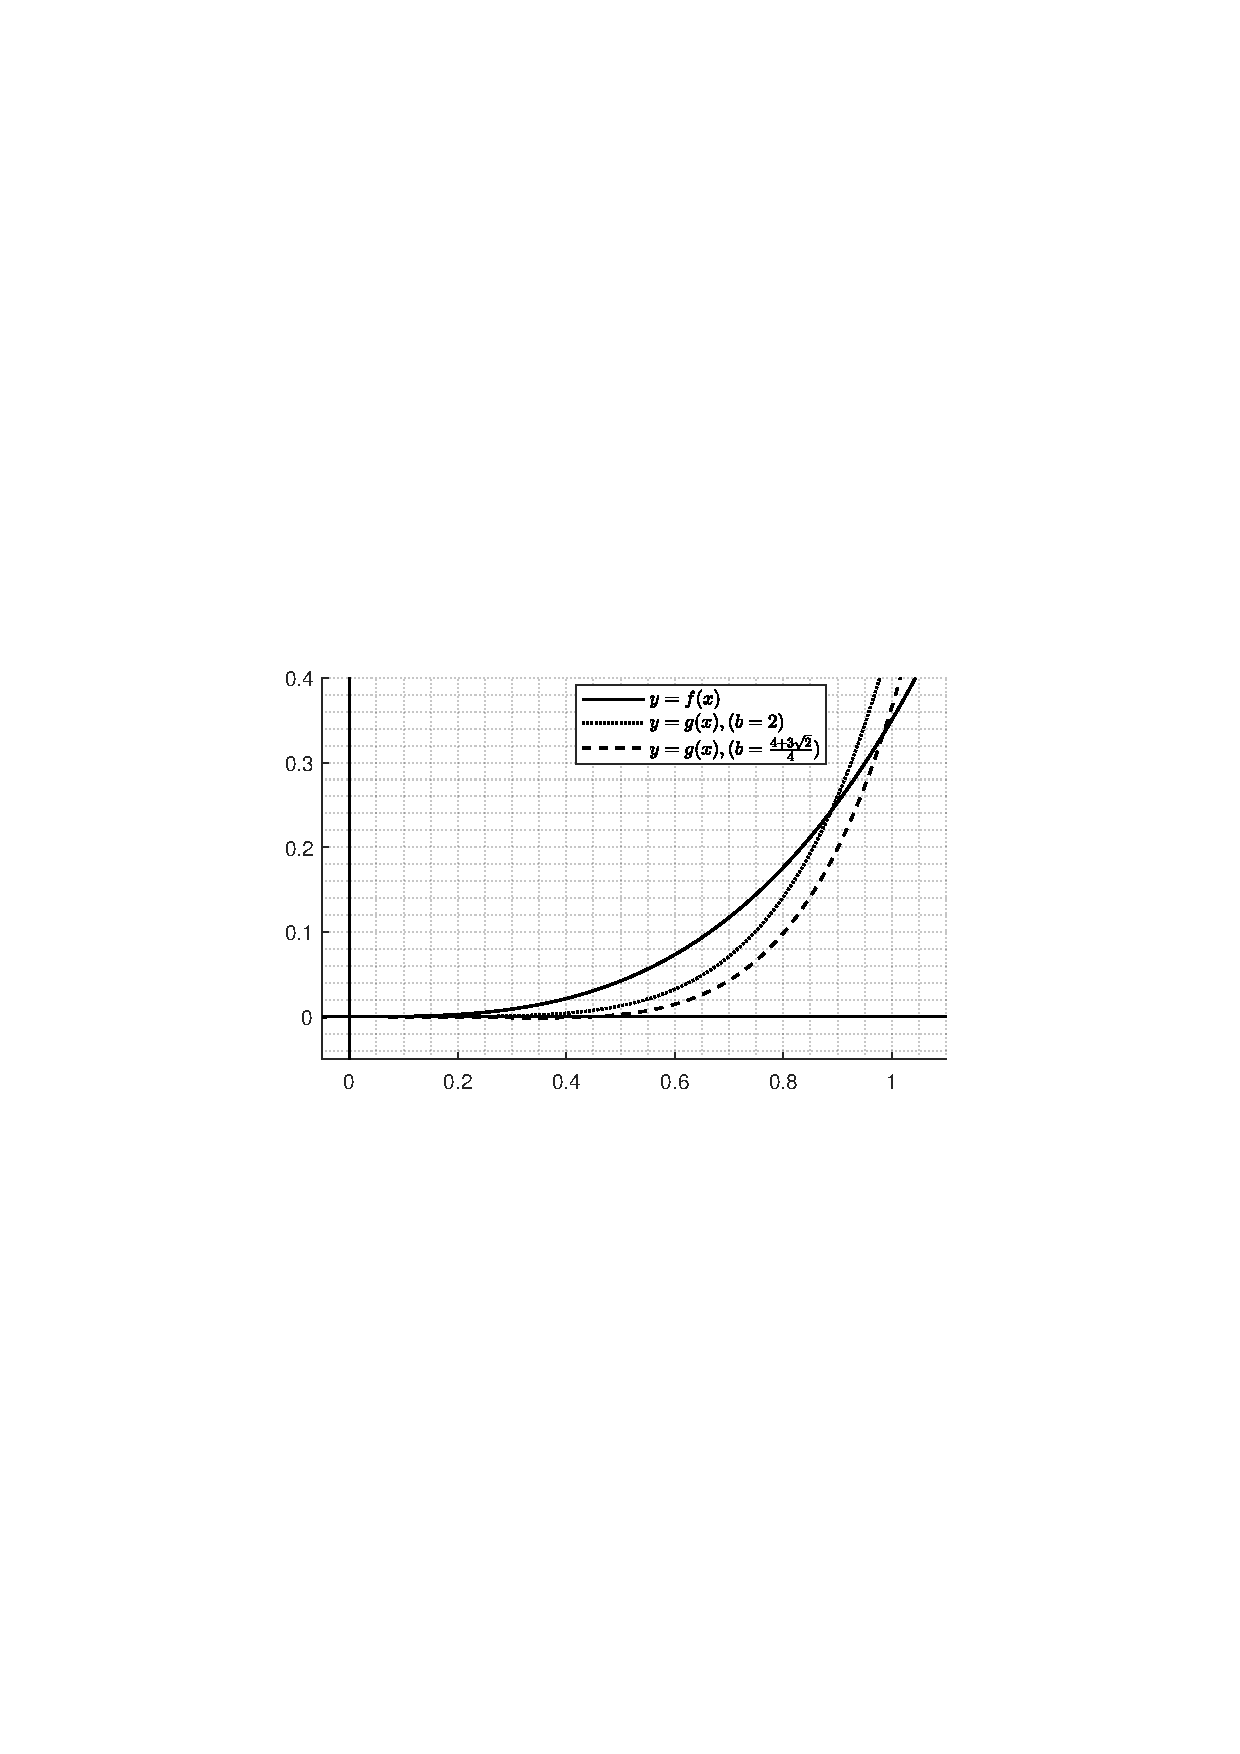
\includegraphics[width=0.6\linewidth]{2014新课标全国II卷}
\end{figure}

$ f(2x) $在原点处的5次泰勒展开为$ \dfrac{8}{3}x^3+\dfrac{8}{15}x^5 $;
当$ b=2 $时,$ 8f(x) $在原点处的5次泰勒展开为$ \dfrac{8}{3}x^3
+\dfrac{2}{15}x^5 $,所以,$ b=2 $的效果就是让$ f(2x)-4bf(x) $
在原点处的泰勒展开没有3次项。

\item (2019,浙江高考)已知实数$ a\neq 0 $,
设函数$ f(x)=a\ln x+\sqrt{x+1},\ (x>0) $.\\
(I) 当$ a=-\dfrac{3}{4} $时,求函数$ f(x) $的单调区间;\\
(II) 对任意$ x\in \Big[\dfrac{1}{\e^2},+\infty\Big) $
均有$ f(x)\leq \dfrac{\sqrt{x}}{2a} $,求$ a $的取值范围。\\
\textbf{解}\ (I) 令$ f'(x)=-\dfrac{3}{4x}+\dfrac{1}{2\sqrt{x+1}}=0 $,
有$ 4x^2-9x-9=(4x+3)(x-3)=0 $,$ f(x) $在$ (0,3) $上单调递减,
在$ (3,+\infty) $上单调递增。\\
(II) 这一小问在高考考场上属于非常困难的题目,但如果允许使用计算机,
则有通法可以解决,毫无难度,所以本题不算精彩,不值得深入研究。
通法就是分离变量,然后求函数极值。

首先,当$ x\geq 1 $时,$ \sqrt{x}<a\ln x+\sqrt{x+1}\leq 
\dfrac{\sqrt{x}}{2a} $,所以$ 1<\dfrac{1}{2a},\ 0<a<\dfrac{1}{2} $. \\
再将$ a\ln x+\sqrt{x+1}\leq \dfrac{\sqrt{x}}{2a} $变为
\begin{gather}\label{2019浙江恒成立}
    a^2\ln x+a\sqrt{x+1}-\frac{1}{2}\sqrt{x}\leq 0
\end{gather}
\textbf{方法一}\ 当$ x=1 $时,$ a\sqrt{2}-\dfrac{1}{2}\leq 0,\ a\leq 
\dfrac{\sqrt{2}}{4} $;当$ x\neq 1 $时,把(\ref{2019浙江恒成立})式
看成关于$ a $的二次不等式。\\
\mycircled{1} 若$ \Delta=x+1+2\sqrt{x}\ln x\leq 0 $,则二次项系数$ \ln x<0 $,
(\ref{2019浙江恒成立})式对任意的$ a $成立。此时$ x $的范围是$ \Big[\dfrac{1}{\e^2},
0.307655\cdots\Big] $.(若没有计算机,则难以求出$ 0.307655\cdots $这一结果,
但即使求不出来,也没有太大影响。) \\
\mycircled{2} 若$ \Delta>0 $,即$ x\in(0.307655\cdots,1)\bigcup(1,+\infty) $,
则求解不等式(\ref{2019浙江恒成立})的结果如下:
\begin{gather*}
    0<a\leq \frac{-\sqrt{x+1}+\sqrt{x+1+2\sqrt{x}\ln x}}{2\ln x}
    \q (\text{将此函数定义为}h(x) )
\end{gather*}
这样就实现了分离变量,手工对$ h(x) $求导和求极值是相当困难的,但借助电脑可轻松得到,
$ h(x) $在$ (0.307655\cdots,1) $上递减,在$ (1,+\infty) $上递增,当$ x\to 1 $
时取得最小值$ \dfrac{\sqrt{2}}{4} $(需要处理一个
$ \dfrac{0}{0} $型的极限,下面的(\ref{2019浙江根号缩放})和
(\ref{2019浙江00极限计算})式实际上就是在计算这个极限),
所以$ a $的范围是$ \Big(0,\dfrac{\sqrt{2}}{4}\Big] $. 

如果没有计算机,也有办法,利用不等式$ \sqrt{1+x}< 
1+\dfrac{1}{2}x\ (x\geq -1,x\neq 0) $,
\begin{align}
    \sqrt{x+1+2\sqrt{x}\ln x} 
    &=\sqrt{x+1}\sqrt{1+\frac{2\sqrt{x}\ln x}{x+1}} \nonumber \\
    & <\sqrt{x+1}\left(1+\frac{\sqrt{x}\ln x}{x+1}\right)=
    \sqrt{x+1}+\frac{\sqrt{x}\ln x}{\sqrt{x+1}} \label{2019浙江根号缩放}
\end{align}
所以,当$ \ln x>0,\ x>1 $时,有
\begin{align}\label{2019浙江00极限计算}
    0<a\leq \frac{-\sqrt{x+1}+\sqrt{x+1+2\sqrt{x}\ln x}}{2\ln x}
    <\dfrac{\dfrac{\sqrt{x}\ln x}{\sqrt{x+1}}}{2\ln x}=
    \frac{\sqrt{x}}{2\sqrt{x+1}}
\end{align}
$ \dfrac{\sqrt{x}}{2\sqrt{x+1}} $在$ (1,+\infty) $上单调递增,
同时,$ \lim\limits_{x\to 1}h(x)=
\lim\limits_{x\to 1}\dfrac{\sqrt{x}}{2\sqrt{x+1}}=
\dfrac{\sqrt{2}}{4} $.所以,当$ x>1 $时,$ a\leq \dfrac{\sqrt{2}}{4} $.
但对于$ x\in(0.307655,1) $,如果不知道单调性,则没有特别简单的方法求$ h(x) $的最小值。
\\
\textbf{方法二}\ 当$ x=1 $时,$ a\leq \dfrac{\sqrt{2}}{4} $;
当$ x\neq 1 $时,如果把(\ref{2019浙江恒成立})式看成关于$ a $的二次函数,
那么对称轴是$ -\dfrac{\sqrt{x+1}}{2\ln x} $,然而,难以判断对称轴与
$ \dfrac{\sqrt{2}}{4} $的相对大小(手工无法求解方程$ -\dfrac{
    \sqrt{x+1}}{2\ln x}=\dfrac{\sqrt{2}}{4} $,借助计算机可解得
$ x=0.210929\cdots $),所以,高考标准答案采用的方法是,
把(\ref{2019浙江恒成立})式除以$ -\dfrac{1}{2}a^2 $,再作代换
$ t=\dfrac{1}{a}\geq 2\sqrt{2} $,然后考虑关于$ t $的二次函数,
令
\begin{gather*}
    g(t)=t^2\sqrt{x}-2t\sqrt{x+1}-2\ln x=\sqrt{x}\left(t-
    \sqrt{1+\frac{1}{x}}\right)^2-\frac{1+x}{\sqrt{x}}-2\ln x
\end{gather*}
此时,就很容易判断$ g(t) $的对称轴与$ 2\sqrt{2} $的相对大小。\\
\mycircled{1} 当$ x\in \Big[\dfrac{1}{7},+\infty\Big) $时,
$ \sqrt{1+\dfrac{1}{x}}\leq 2\sqrt{2} $,则
\begin{gather*}
    g(t)\geq g(2\sqrt{2})=8\sqrt{x}-4\sqrt{2}\sqrt{x+1}-2\ln x
\end{gather*}
令$ p(x)=4\sqrt{x}-2\sqrt{2}\sqrt{x+1}-\ln x $,则
\begin{align}
    p'(x)=\frac{2}{\sqrt{x}}-\frac{\sqrt{2}}{\sqrt{x+1}}-
    \frac{1}{x} &=\frac{2\sqrt{x}\sqrt{x+1}-\sqrt{2}x-
        \sqrt{x+1}}{x\sqrt{x+1}}\label{2019浙江根式方程}\\ 
    &=\frac{(x-1)[1+\sqrt{x}(\sqrt{2 x+2}-1)]}{x 
        \sqrt{x+1}(\sqrt{x}+1)(\sqrt{x+1}+\sqrt{2 x})}
    \label{2019浙江复杂因式分解}
\end{align}
显然,$ p(x) $在$ \Big[\dfrac{1}{7},1\Big] $上单调递减,在
$ (1,+\infty) $上单调递增,在$ x=1 $处取得极小值。所以
$ p(x)\geq p(1)=0 $,进而$ g(t)\geq g(2\sqrt{2})=2p(x)\geq 0 $.\\
\mycircled{2} 当$x\in\Big[\dfrac{1}{\e^{2}},\dfrac{1}{7}\Big)$时,
$ g(t)\geqslant g\Big(\sqrt{1+\dfrac{1}{x}}\Big)=\dfrac{-2\sqrt{x}
    \ln x-(x+1)}{\sqrt{x}}$,\\
令$ q(x)=2\sqrt{x}\ln x+(x+1),\ x\in\Big[\dfrac{1}{\e^{2}},
\dfrac{1}{7}\Big] $,则$ q'(x)=\dfrac{\ln x+2}{\sqrt{x}}+1>0 $,
故$q(x)$在$\Big[\dfrac{1}{\e^{2}},\dfrac{1}{7}\Big]$上单调递增,
所以,
\begin{gather}
    q(x)\leqslant q\Big(\dfrac{1}{7}\Big)=-\frac{2}{\sqrt{7}}
    \ln 7+\frac{8}{7}=-\dfrac{2\sqrt{7}}{7} p\Big(\dfrac{1}{7}\Big)<-\dfrac{2\sqrt{7}}{7} p(1)=0 
    \label{2019浙江估计q(1_7)}\\
    g(t)\geqslant g\Big(\sqrt{1+\dfrac{1}{x}}\Big)=
    -\dfrac{q(x)}{\sqrt{x}}>0 \nonumber
\end{gather}
由\mycircled{1},\mycircled{2}知,对任意$ x\in\Big[\dfrac{1}{\e^{2}},
+\infty\Big),\ t\in[2\sqrt{2}, +\infty)$,$ g(t)\geqslant 0 $,
即对任意$ x\in\Big[\dfrac{1}{\e^{2}},+\infty\Big)$,均有
$ f(x)\leqslant\dfrac{\sqrt{x}}{2a} $.

综上所述,$ a $的取值范围是$ \Big(0,\dfrac{\sqrt{2}}{4}\Big] $. \\
\textbf{注1}:(\ref{2019浙江复杂因式分解})式分子中的因式分解很难想出来,
是本题的难点之一。虽然可以尝试直接解方程$ 2\sqrt{x}\sqrt{x+1}-
\sqrt{2}x-\sqrt{x+1}=0 $,但还是会遇到困难。
\begin{gather*}
    2\sqrt{x}\sqrt{x+1}=\sqrt{2}x+\sqrt{x+1}\q (\text{两边平方}) \\
    4x(x+1)=2x^2+2\sqrt{2}x\sqrt{x+1}+x+1 \\
    2x^2+3x-1=2\sqrt{2}x\sqrt{x+1} \q (\text{两边平方}) \\
    4x^4+4x^3-3x^2-6x+1=0 \q (\text{测试比较小的整数是否为根})\\
    (x-1)(4x^3+8x^2+5x-1)=0
\end{gather*}
其中,$ 4x^3+8x^2+5x-1 $在$ (0,+\infty) $上单调递增,
但在$ \Big[\dfrac{1}{7},1\Big] $上有一个零点$ 0.157298\cdots $\\ (手算比较困难),
更麻烦的是,这个零点不是$ 2\sqrt{x}\sqrt{x+1}-
\sqrt{2}x-\sqrt{x+1} $的零点,所以也不是$ p'(x) $
的零点。那它是什么函数的零点呢?其实是$ 2\sqrt{x}\sqrt{x+1}+
\sqrt{2}x-\sqrt{x+1} $的零点。$ \pm 2\sqrt{x}\sqrt{x+1}\pm 
\sqrt{2}x\pm \sqrt{x+1}=0 $似乎共有8个方程,但只有4个不同的方程
(比如三处$ \pm $全部取$ + $与全部取$ - $得到的两个方程实际上是同一个),
这4个不同的方程经过上面的平方、移项步骤后都会得到$ 4x^4+4x^3-3x^2-6x+1=0 $.
这些步骤与第\pageref{x4-10x2+1}页展示的求$ x=\sqrt{2}+\sqrt{3} $
所满足的整系数方程的步骤基本是一样的。\\
\textbf{注2}:(\ref{2019浙江估计q(1_7)})式中判断$ q\Big(\dfrac{1}{7}\Big) $
的正负的方法也不容易想到,更容易的想法是直接算出数值。
$ \ln 7 $可以按(\ref{ln7估算方法})式的方法估算,约为$ 1.960 $.
如果记得住$ \ln 7 $,那么直接使用$ \ln 7\approx 1.946 $.
另外,$ \sqrt{7}\approx 2.646 $是需要记住的数字,然后
\begin{gather*}
    q\Big(\dfrac{1}{7}\Big)=-\frac{2}{\sqrt{7}}\ln 7+\frac{8}{7}
    \approx -\frac{2}{2.646}\times 1.960+1.143\approx -0.338<0
\end{gather*}
$ q\Big(\dfrac{1}{7}\Big) $的精确值是$ -0.328\cdots $,以上估算方法精度足够。
希望读者能记住$ \ln2,\ln3,\ln5,\ln7 $和$ \sqrt{2}\sim \sqrt{10} $. \\
\textbf{注3}:$ q(x) $中出现了$ \sqrt{x}\ln x $,这个函数在黎曼猜想的
一种等价形式中也出现了。
设$ \pi(x) $表示小于等于$ x $的质数的个数(这个函数是不光滑的,
存在很多“台阶”,每经过一个质数,函数值才会加1,写不出精确的表达式)。
$ \disp \mathrm{Li}(x)=\int_2^{x}\dfrac{\d t}{\ln t} $为对数积分函数
(无法写成基本初等函数,或者说写不出显式表达式),那么黎曼猜想成立等价于
\begin{gather*}
    \pi(x)=\mathrm{Li}(x)+O(\sqrt{x}\ln x)
\end{gather*}
其中$ O(\sqrt{x}\ln x) $的含义是:若$ \lim\limits_{x\to+\infty}\left|
\dfrac{F(x)}{\sqrt{x}\ln x}\right|\leq A\ (A>0) $,
则$ F(x)=O(\sqrt{x}\ln x) $. 

\item $ ^* $(2008,江西高考)定义函数$ f(x)=\dfrac{1}{\sqrt{1+x}}+
\dfrac{1}{\sqrt{1+a}}+\sqrt{\dfrac{ax}{ax+8}} $,$ x>0 $. \\
(1)当$ a=8 $时,求$ f(x) $的单调区间;\\
(2)对任意$ a>0 $,求证:$ 1<f(x)<2 $. \\
\textbf{说明}\ 此题第(2)问的难度在中国历年高考数学题中可以排进前三,
当年的江西考生无人拿满分,它起源于2004年中国西部数学竞赛(王建伟供题),
对任意正实数$ a,b,c $,求证:
\begin{gather*}
    1<\dfrac{a}{\sqrt{a^2+b^2}}+\dfrac{b}{\sqrt{b^2+c^2}}+
    \dfrac{c}{\sqrt{c^2+a^2}}\leq \dfrac{3\sqrt{2}}{2} 
\end{gather*}
上式等价于
\begin{gather*}
    1<\dfrac{1}{\sqrt{1+\dfrac{b^2}{a^2}}}+\dfrac{1}{\sqrt{1+\dfrac{c^2}{b^2}}}+
    \dfrac{1}{\sqrt{1+\dfrac{a^2}{c^2}}}\leq \dfrac{3\sqrt{2}}{2} 
\end{gather*}
若引入变量$ u=\dfrac{b^2}{a^2},v=\dfrac{c^2}{b^2},w=\dfrac{a^2}{c^2} $,则$ uvw=1 $.\\
对于这道高考题的第(2)问,受第(1)问的引导(或误导),最直接的想法仍然是求导后找零点,
\begin{gather*}
    f'(x)=-\dfrac{1}{2(1+x)^{3/2}}+\dfrac{4\sqrt{a}}{\sqrt{x}(ax+8)^{3/2}}=0 \\
    x(ax+8)^3=64a(1+x)^3 \\
    a^3x^4+24a^2x^3-64ax^3-192ax-64a+512x=0\\
    (ax^2-8)(a^2x^2+24ax-64x+8a)=0
\end{gather*}
最后这个因式分解并不容易看出来,即使能看出来,也只有$ x=\sqrt{\dfrac{8}{a}} $(舍弃负值)
这个解的表达式比较简单。对于$ a^2x^2+24ax-64x+8a=0 $,判别式
\begin{align}\label{判别式(a-2)(a-8)2}
    \Delta=(24a-64)^2-32a^3=-32(a-2)(a-8)^2
\end{align}
第(1)问中取$ a=8 $,比较简单。
但对于第(2)问,并不能确定判别式(\ref{判别式(a-2)(a-8)2})的正负号,二次方程未必有实根。
即使有实根,表达式也过于复杂,无法继续计算。所以,必须转变思路,另辟蹊径。\\
\\
先证$ f(x)>1 $. \\
\textbf{方法一}\ 判别式(\ref{判别式(a-2)(a-8)2})已经提示我们,$ a=2 $是一个关键的分界点,
所以可设法比较$ f(x) $与$ \dfrac{1}{\sqrt{1+x}}+\sqrt{\dfrac{x}{4+x}} $的大小。
不妨设$ x\leq a\leq \dfrac{8}{ax} $,因为$ x\cdot a\cdot\dfrac{8}{ax}
=8 $,所以,$ x,a,\dfrac{8}{ax} $三者不可能同时大于2或同时小于2,于是,$ x\leq 2\leq \dfrac{8}{ax} $.若$ a\geq 2 $,那么$ \dfrac{4}{x}\geq \dfrac{8}{ax}\geq 2 $;
若$ a<2 $,那么$ \dfrac{4}{x}\geq 2>a $.
于是
\begin{align*}
    f(x)=\dfrac{1}{\sqrt{1+x}}+\dfrac{1}{\sqrt{1+a}}+\dfrac{1}{\sqrt{1
            +\dfrac{8}{ax}}} >\dfrac{1}{\sqrt{1+x}}+\dfrac{1}{\sqrt{1+\dfrac{4}{x}}} 
    =\dfrac{\sqrt{4+x}+\sqrt{x^2+x}}{\sqrt{(1+x)(4+x)}} 
\end{align*}
通过平方容易验证$ \sqrt{4+x}+\sqrt{x^2+x}>\sqrt{(1+x)(4+x)} $,所以$ f(x)>1 $.\\
\textbf{方法二}\ 设$ b=\dfrac{8}{ax} $,则
\begin{align*}
    f(x)>&\dfrac{1}{1+x}+\dfrac{1}{1+a}+\dfrac{1}{1+b} \\
    =&\dfrac{2a+2b+2x+ab+ax+bx+3}{a+b+x+ab+ax+bx+abx+1} \\
    =&\ 1+\dfrac{a+b+x-6}{a+b+x+ab+ax+bx+9}
\end{align*}
因为$ a+b+x\geq 3\sqrt[3]{abx}=6 $,所以$ f(x)>1 $. \\
\textbf{方法三}\ 设$ X=\dfrac{1}{\sqrt{1+x}}<1,\ A=\dfrac{1}{\sqrt{1+a}}<1,
\ B=\dfrac{1}{\sqrt{1+b}}<1 $,那么
\begin{align*}
    8X^2A^2B^2=&\dfrac{8}{(1+x)(1+a)(1+b)}\\
    =&\dfrac{xab}{(1+x)(1+a)(1+b)}=(1-X^2)(1-A^2)(1-B^2)
\end{align*}
用反证法,假设$ f(x)=X+A+B\leq 1 $,那么$ A+B\leq 1-X $,
\begin{align*}
    2X(A+B)\leq 2X(1-X)<(1+X)(1-X)=1-X^2
\end{align*}
同理可得,$ 2A(X+B)<1-A^2,\ 2B(X+A)<1-B^2 $,三式相乘可得
\begin{gather*}
    8XAB(A+B)(X+B)(X+A)<(1-X^2)(1-A^2)(1-B^2)=8X^2A^2B^2 \\
    (A+B)(X+B)(X+A)<XAB
\end{gather*}
但$ (A+B)(X+B)(X+A)\geq 2\sqrt{AB}\cdot 2\sqrt{XB}\cdot 2\sqrt{XA}=8XAB $,
产生了矛盾,所以$ f(x)=X+A+B>1 $.\\
\\
再证$ f(x)<2 $. \\
\textbf{方法一}\ 用反证法,假设$ f(x)=X+A+B\geq 2 $,那么$ A+B-1\geq 1-X $,
另外,$ (1-A)(1-B)>0 $,所以$ AB>A+B-1\geq 1-X $,
\begin{align*}
    (1-X^2)=(1+X)(1-X)<2(1-X)<2AB
\end{align*}
同理可得,$ 1-A^2<2XB,\ 1-B^2<2XA $,三式相乘可得
\begin{align*}
    (1-X^2)(1-A^2)(1-B^2)<8X^2A^2B^2
\end{align*}
产生了矛盾,所以$ f(x)=X+A+B<2 $. \\
\textbf{方法二}\ 不妨设$ x\leq a\leq b $,那么$ 0<x\leq 2 $. \\
I.当$ x+a\geq 7 $时,$ b\geq a\geq 5 $,那么
\begin{gather*}
    \dfrac{1}{\sqrt{1+x}}<1,\ \dfrac{1}{\sqrt{1+a}}+\dfrac{1}{\sqrt{1+b}}\leq
    \dfrac{2}{\sqrt{1+5}}<1
\end{gather*}
所以,$ f(x)=\dfrac{1}{\sqrt{1+x}}+\dfrac{1}{\sqrt{1+a}}+\dfrac{1}{\sqrt{1+b}}<2 $. \\
II.当$ x+a<7 $时,
\begin{gather*}
    \dfrac{1}{1+x}=1-\dfrac{x}{1+x}<1-\dfrac{x}{1+x}+\dfrac{x^2}{4(1+x)^2}=\left[
    1-\dfrac{x}{2(1+x)}\right]^2 \\
    \dfrac{1}{\sqrt{1+x}}<1-\dfrac{x}{2(1+x)}
\end{gather*}
同理可得:$ \dfrac{1}{\sqrt{1+a}}<1-\dfrac{a}{2(1+a)} $.于是,
\begin{align*}
    f(x)<2-\dfrac{1}{2}\left(\dfrac{x}{1+x}+\dfrac{a}{1+a}-
    2\sqrt{\dfrac{ax}{ax+8}}\right)
\end{align*}
又因为
\begin{align*}
    \dfrac{x}{1+x}+\dfrac{a}{1+a}\geq 2\sqrt{\dfrac{ax}{(1+x)(1+a)}}
    =2\sqrt{\dfrac{ax}{1+a+x+ax}}>2\sqrt{\dfrac{ax}{ax+8}}
\end{align*}
所以,$ f(x)<2 $成立。

事实上,结论可加强为$ 1<f(x)\leq \sqrt{3} $.当$ x=a=\dfrac{8}{ax}=2 $时,
$ f(x)=\sqrt{3} $. 证明过程参见脚注中的文献\footnote{王品行.2008年高考数学江西理科卷压轴题之别解[J].中学数学研究,2008:24-25.\\ 蒋明斌.一道西部数学奥林匹克赛题的溯源与推广[J].中学数学研究,2006:50-52.\\
    吴善和.关于IMO42一个不等式的逆向[J].中学数学研究,2004:50-50}。
从高等数学角度来讲,实际上是研究二元函数$ F(x,a)=\dfrac{1}{\sqrt{1+x}}+
\dfrac{1}{\sqrt{1+a}}+\sqrt{\dfrac{ax}{ax+8}} $在$ x>0,a>0 $时的极值,
或者是三元函数$ G(x,a,b)=\dfrac{1}{\sqrt{1+x}}+\dfrac{1}{\sqrt{1+a}}+
\dfrac{1}{\sqrt{1+b}} $在约束条件$ xab=8 $下的极值,
可采用拉格朗日未定乘数法,然后求二重极限。

% exp_taylor.m
\item $ ^* $(2012,华约自主招生;2022,中科大少年班招生) 记$ S_n(x)=\sum\limits_{l=0}^{n}
\dfrac{x^l}{l!}=1+x+\dfrac{x^2}{2!}+\cdots+\dfrac{x^n}{n!} $,
求证:当$ n $为奇数时,$ S_n(x)=0 $有且仅有一个实根,
当$ n $为奇数时,$ S_n(x)=0 $没有实根。\\
\textbf{解}\ 显然,$ S_n(x) $就是$ \e^x $在$ x=0 $处的泰勒展开的截断多项式。
下面将证明:当$ k\geq 1 $时,$ S_{2k-1}(x) $在$ \textbf{R} $上单调递增,
将$S_{2k-1}(x)$唯一的实根记为$ r_{2k-1}$,则数列$ \{r_{2k-1}\} $严格递减且满足
$ -(2k-1)\leq r_{2k-1} <0 $,等号仅在$ k=1 $时取得. $ S_{2k}(x) $在
$ \textbf{R} $上有且仅有一个正的极小值。

将$S_{2k}(x)$的极小值记为$ m_{2k} $,用数学归纳法证明,
当$ k=1 $时,$ S_1(x)=1+x $在$ \textbf{R} $上单调递增,$ r_1=-1 $, $ S_2(x)=1+x+\dfrac{x^2}{2} $有一个极小值,$ m_2=S_2(-1)=\dfrac{1}{2}>0 $. 假设$ k=t $时结论成立,则当$ k=t+1 $时,$ S'_{2t+1}(x)=S_{2t}(x)\geq m_{2t}>0 $在$ \textbf{R} $恒成立,故$ S_{2t+1}(x) $在$ \textbf{R} $上单调递增,它存在唯一实零点$ r_{2t+1}$. $ S'_{2t+2}(x)=S_{2t+1}(x) $在$(-\infty,r_{2t+1}) $上为负,在$(r_{2t+1},+\infty) $上为正。因此
\begin{align*}
    m_{2t+2}=S_{2t+2}(r_{2t+1})=S_{2t+1}(r_{2t+1})+\dfrac{r_{2t+1}^{2t+2}}{(2t+2)!}=0+\dfrac{r_{2t+1}^{2t+2}}{(2t+2)!}>0
\end{align*}
$ m_{2t+2} $是$ S_{2t+2}(x) $唯一的、正的极小值。
\begin{gather}
    S_{2t-1}(-(2t+1))=S_{2t+1}(-(2t+1))=\sum_{l=0}^{t}\dfrac{{(2t+1)}^{2l}}{(2l)!}\left( 1-\dfrac{2t+1}{2l+1} \right) <0  \label{两条曲线交点} \\
    S_{2t+1}(r_{2t-1})=S_{2t-1}(r_{2t-1})+\dfrac{r_{2t-1}^{2t}}{(2t)!} \left( 1+\dfrac{r_{2t-1}}{2t+1}\right)>0
\end{gather}
又因为$ S_{2t+1}(r_{2t+1})=0 $,所以$ -(2t+1)<r_{2t+1}<r_{2t-1} $.
(\ref{两条曲线交点})式还说明$ (-(2t+1),S_{2t\pm 1}(-(2t+1))) $恰好是$ y=S_{2t+1}(x) $与$ y=S_{2t-1}(x) $两条曲线的交点。同理,$ (-2t,S_{2t}(-2t)) $恰好是$ y=S_{2t}(x) $与$ y=S_{2t-2}(x) $两条曲线的交点。 

$ S_n(x),\ n=2,3,\cdots, 12 $的图像如下:
\begin{figure}[h]
    \centering
    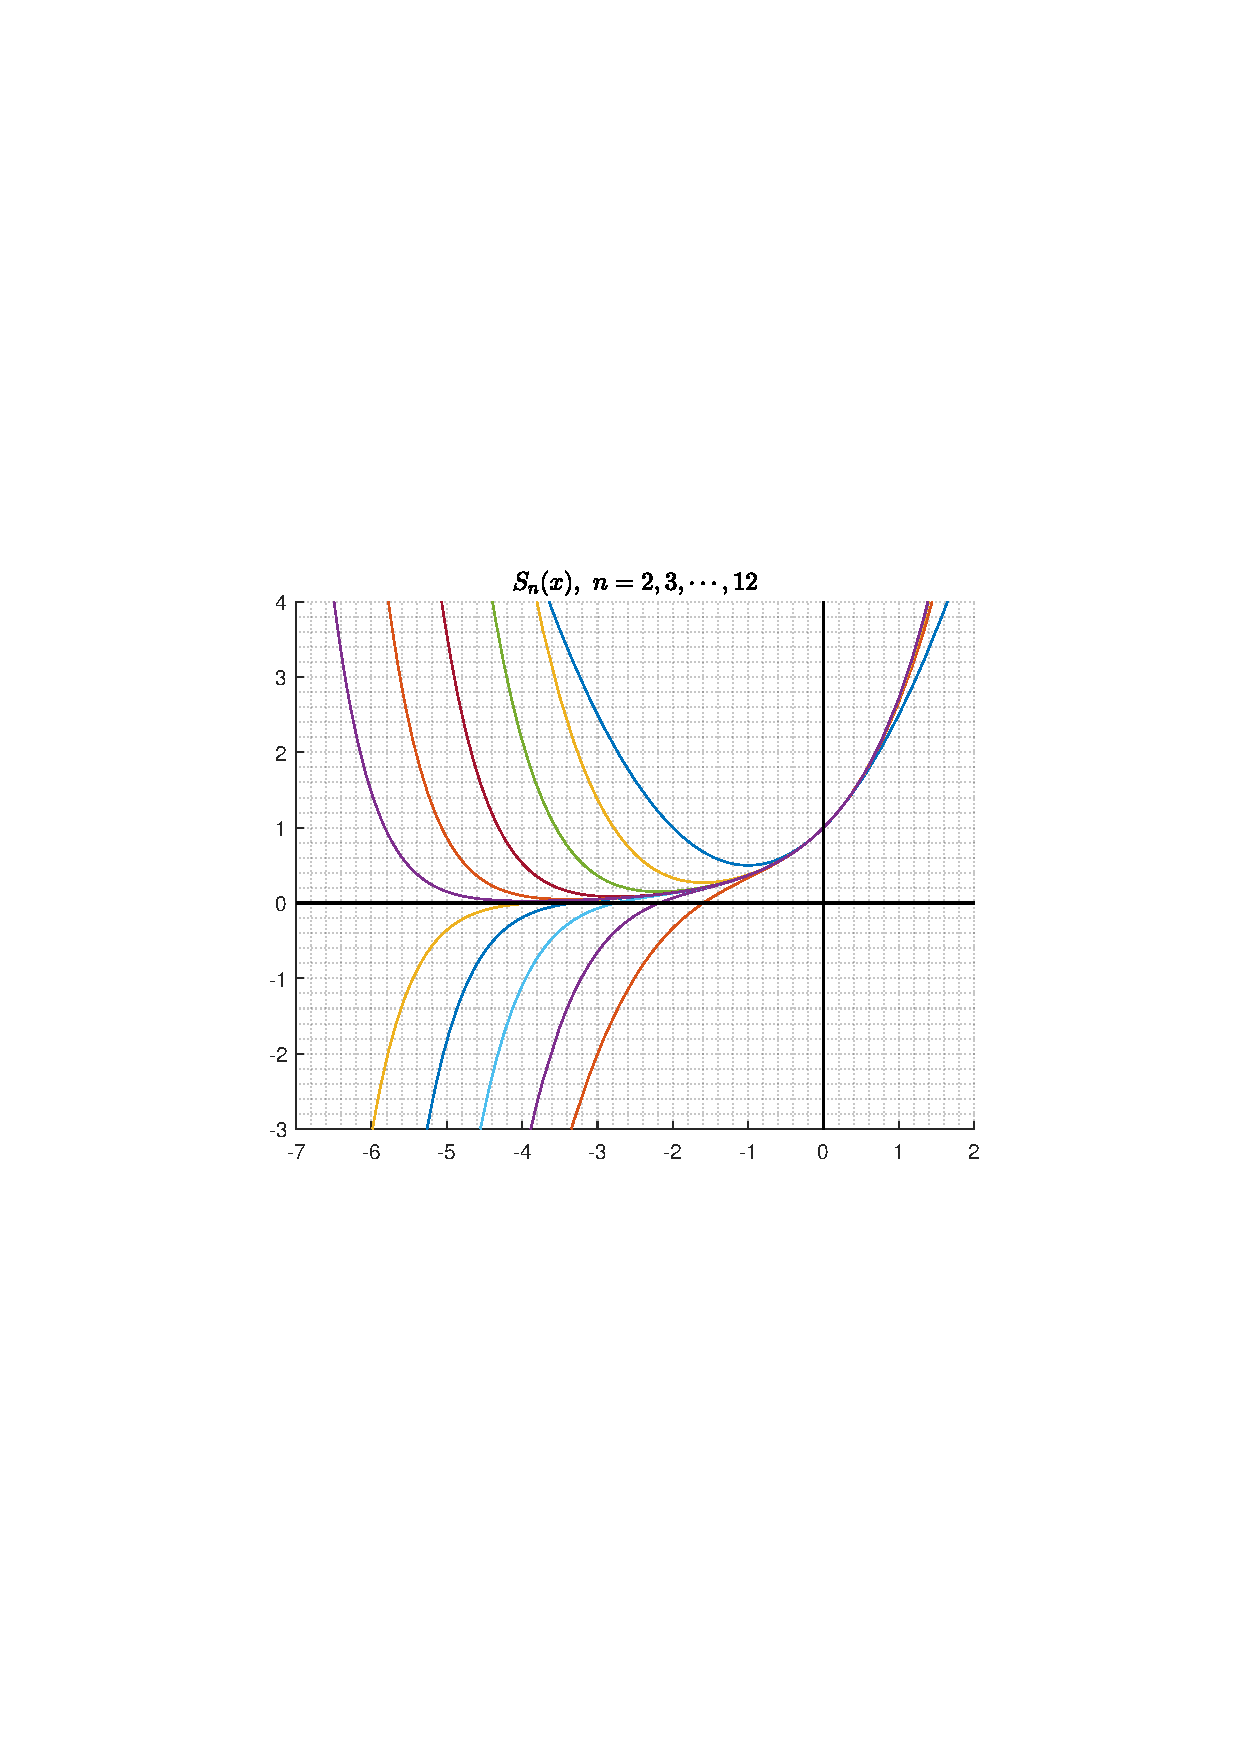
\includegraphics[width=0.6\linewidth]{ex截断多项式图像12}
\end{figure} 

下面来粗略分析$ S_n(x)=0 $的全部根$ Z_{n,j},\ j=1,2 \cdots n $在复平面上的分布情况。
$ n=15,24,33,42,51,60 $时,根的分布情况如下图:
\begin{figure}[h]
    \centering
    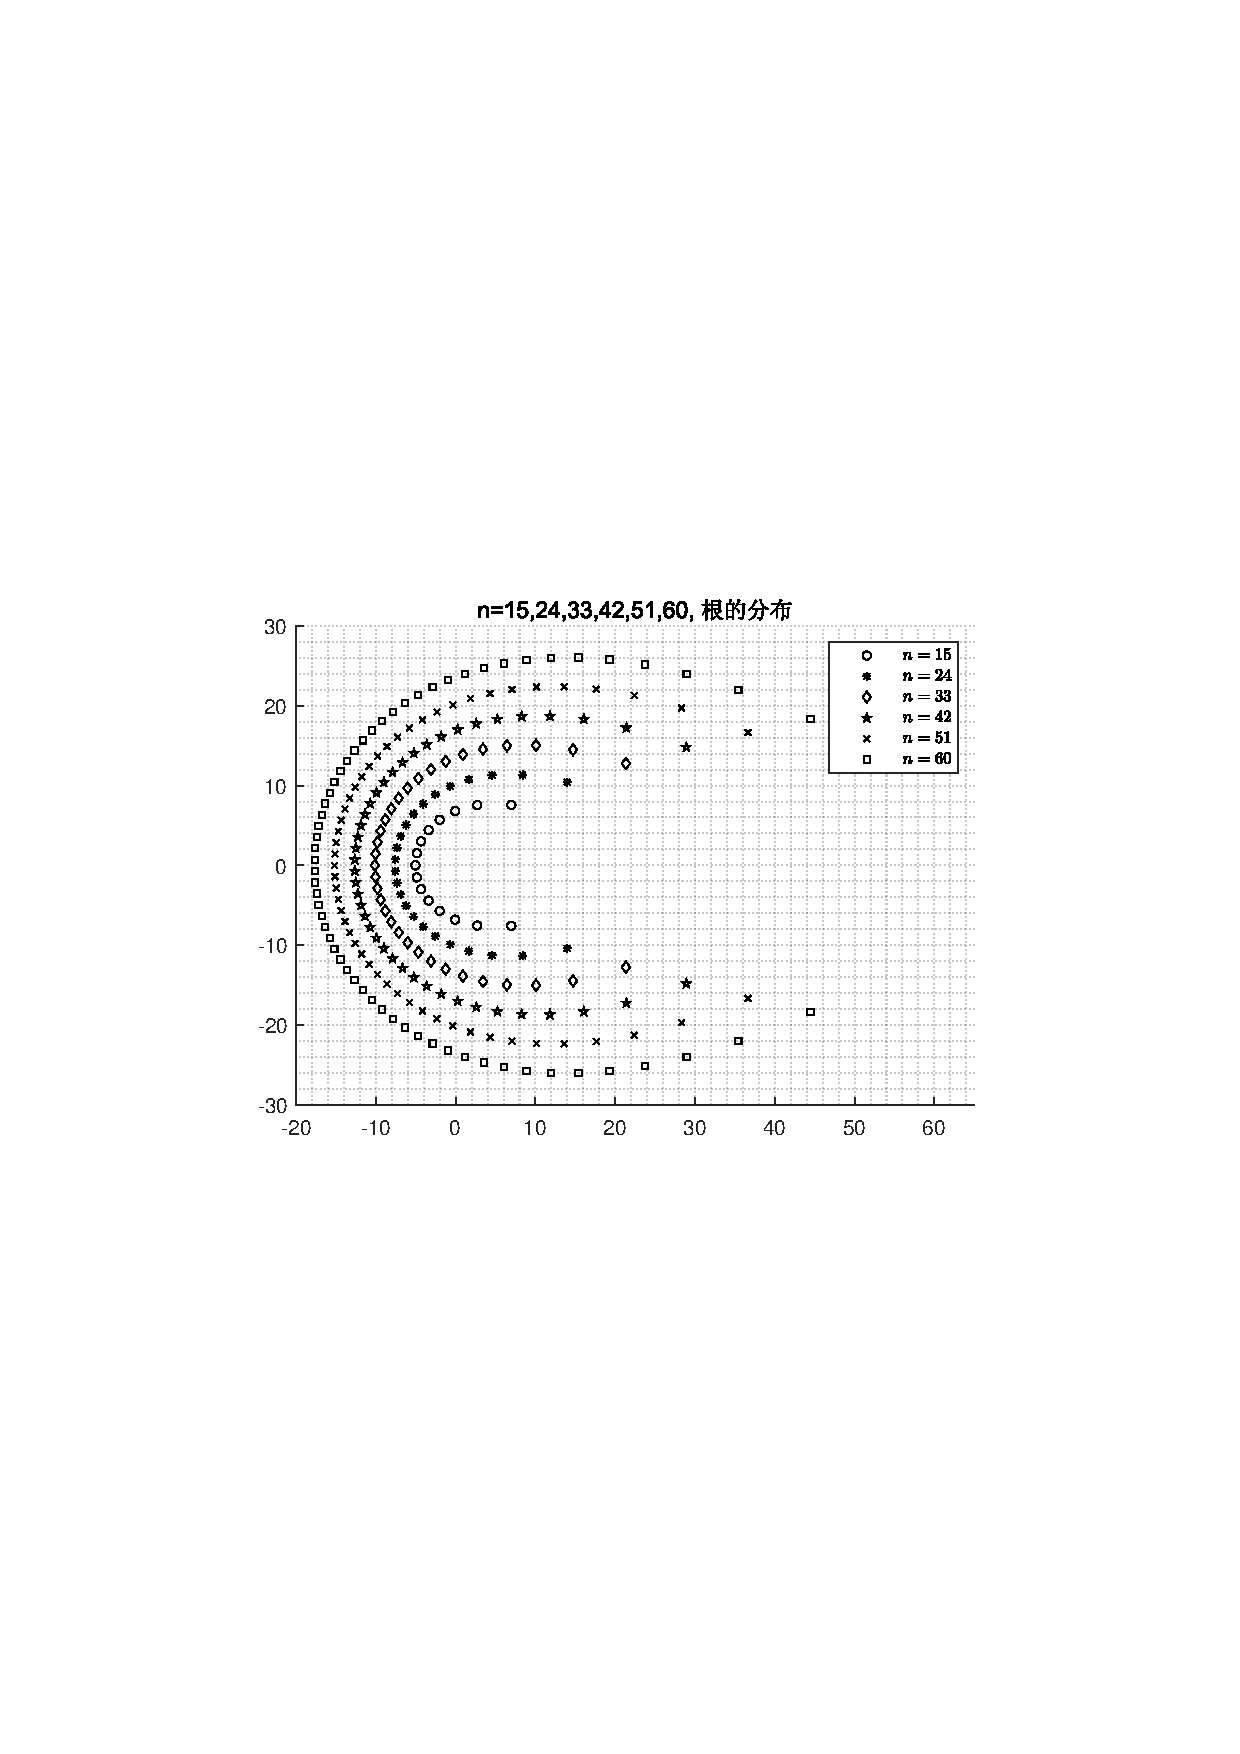
\includegraphics[width=0.6\linewidth]{ex未归一化的根的分布}
\end{figure} 

可以看出这些复数根的模几乎是随$ n $线性增加的。上图也完美地体现了卢卡斯定理
(参看本书第\pageref{Lucas定理-凸包}页):多项式的导数的零点全都落在多项式
本身的零点所形成的凸包之内。

而$ n=2,3,4,\cdots,60 $时,
全部根的分布情况如下图,似乎是落在某些规则的曲线上,相当有趣。
\begin{figure}[h]
    \centering
    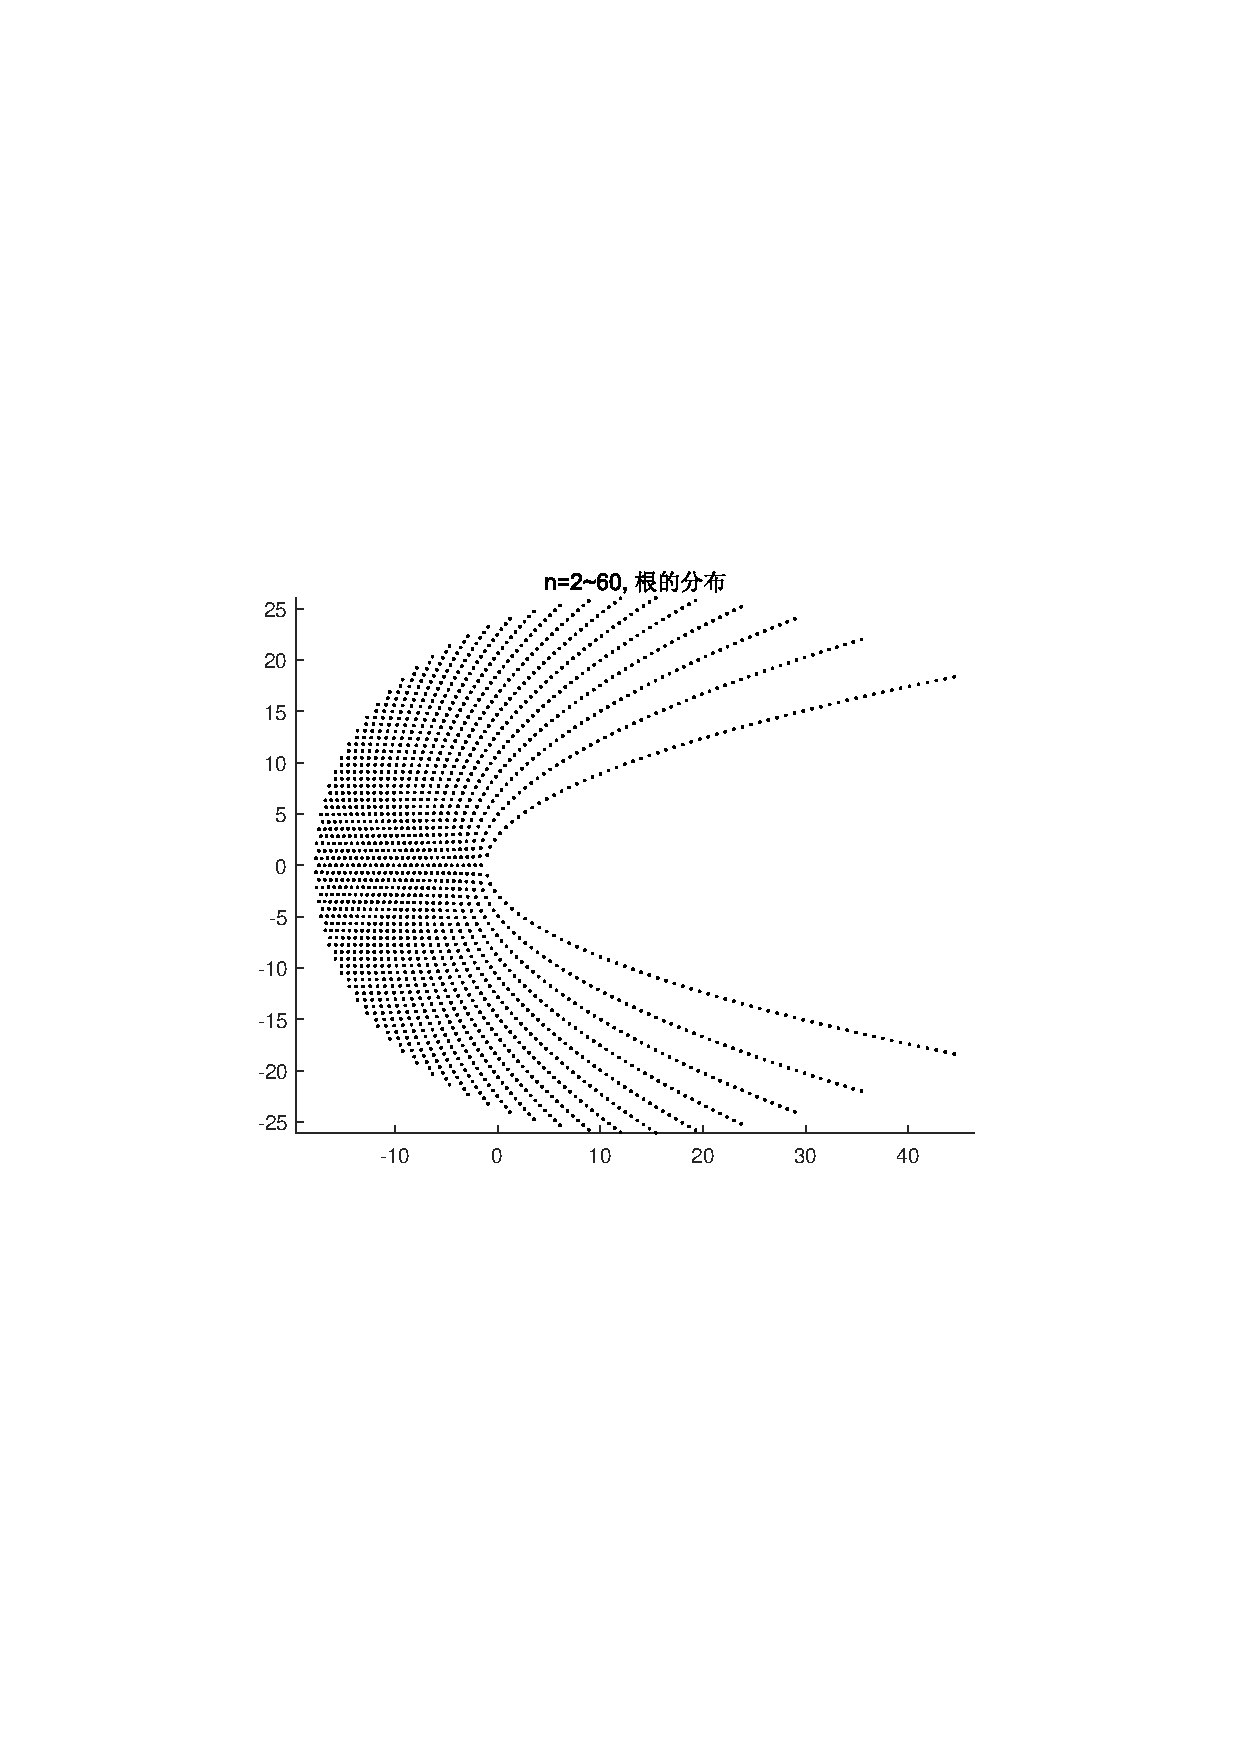
\includegraphics[width=0.6\linewidth]{ex未归一化的根的分布2_60}
\end{figure} 

把$ S_n(x)=0 $的全部根除以$ n $后,再次绘制$ n=24,42,60 $时的分布情况如下图:
\begin{figure}[h]
    \centering
    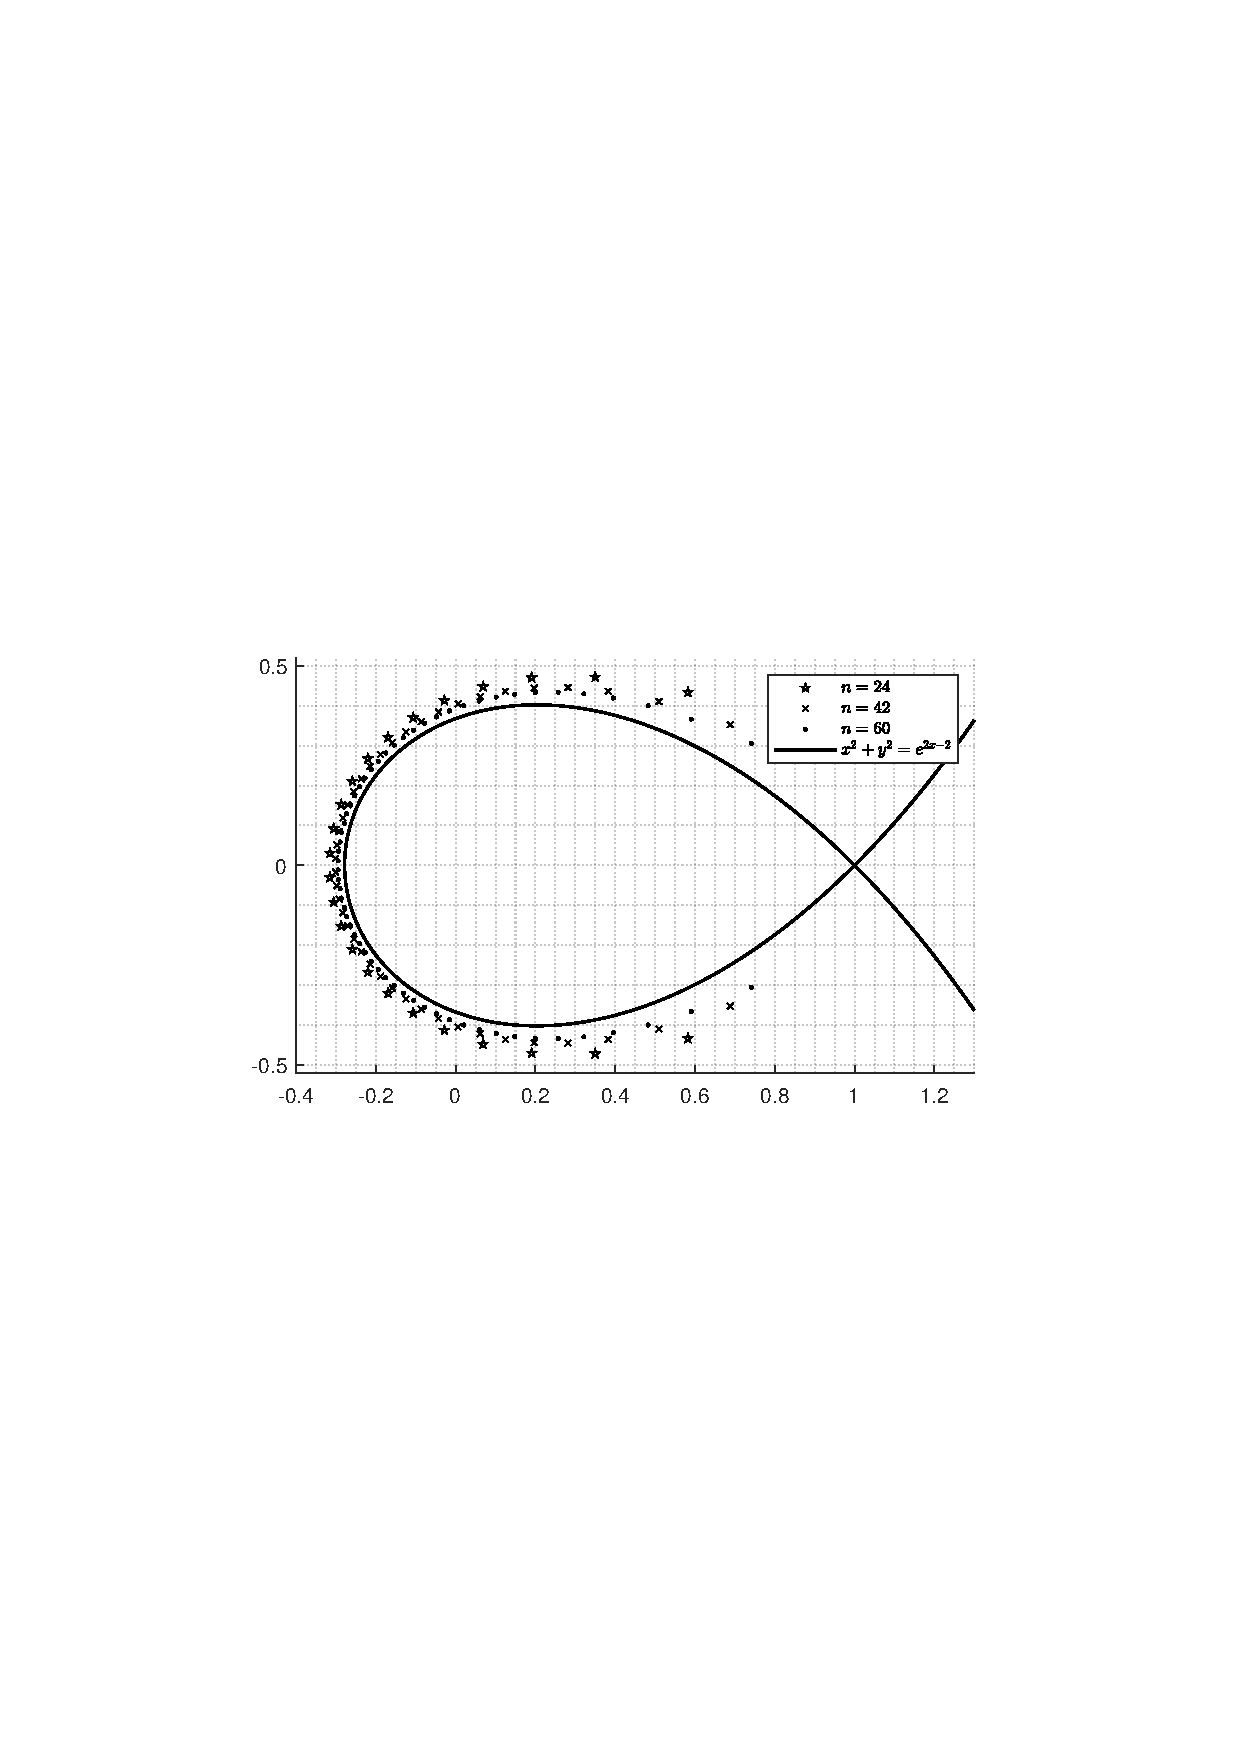
\includegraphics[width=0.6\linewidth]{ex归一化的根的分布}
\end{figure} 

曲线$ x^2+y^2=\e^{2x-2} $被称为Szego曲线\footnote{
    $ \diamond $  G. Szego, Uber eine Eigenschaft der exponentialreihe, Sitzungsberichte der Berliner Math. Gesellschaft 21 (1922) 50–64. \\
    $ \diamond $ R.S. Varga, A.J. Carpenter. Asymptotics for the zeros of the partial sums of $ \e^z $.II. Computational Methods and Function Theory, 1990. \\
    $ \diamond $ Kriecherbauer T,  Kuijlaars A,  Mclaughlin K, et al. Locating the zeros of partial sums of exp(z) with Riemann-Hilbert methods[J]. Mathematics, 2008, 458. \\
    $ \diamond $ Dupuy T,  Mclaughlin D T, SZEGO CURVES, STEEPEST DESCENT ANALYSIS AND THE ZERO BEHAVIOR OF PARTIAL SUMS OF THE EXPONENTIAL FUNCTION, 2005.  \\
    $ \diamond $ Peter Walker. The Zeros of the Partial Sums of the exponential Series.[J]. American Mathematical Monthly, 2003.  \\
    $ \diamond $ Peter Walker, 陆柱家(译), 姚景齐(校). 指数级数部分和的零点[J]. 数学译林, 2008, 27(4):380-381.},
该曲线写成复数形式为$ |z|=|\e^{z-1}| $,或者$ |z\e^{1-z}|=1 $. 可以看出,
复数根除以$ n $之后,全部落在Szego曲线的外部,随着$ n $的增加,
逐渐靠近Szego曲线。得到Szego曲线的关键是利用斯特林(Stirling)公式
\footnote{参见《特殊函数概论》 第108页,($ \Gamma $函数)渐近展开式。},
当$ n $很大时,$ n!\approx \sqrt{2\pi n}\left(\dfrac{n}{\e}\right)^n $. 
在$ x^2+y^2=\e^{2x-2}$中令$ y=0 $,可得到两个解:$ x=1 $或
$ x_0=-W\left(\dfrac{1}{\e}\right)=-0.278464\cdots $,其中的
$ W(x) $代表Lambert W函数。所以:
\begin{align*}
    \lim_{k\to \infty}\dfrac{r_{2k-1}}{2k-1}=-W\left(\dfrac{1}{\e}\right)
    \hspace{2cm}  \lim_{k\to \infty}(r_{2k+1}-r_{2k-1})
    =-2W\left(\dfrac{1}{\e}\right)
\end{align*}
Szego曲线在$ x<1 $时的极值点的横坐标$ x_m $满足方程$ \e^{2x_m-2}=x_m $,于是
$ x_m=-\dfrac{1}{2}W(-\dfrac{2}{\e^2})=0.203187\cdots $,极大值点纵坐标
$ y_m=\sqrt{x_m-x_m^2}=0.402371\cdots $. Szego曲线在$ x\leq x_m $时,
形状接近椭圆,若把$ (x_0,0) $作为椭圆长轴端点,两个极值点作为短轴端点,
此椭圆的方程近似为
\begin{align*}
    \dfrac{(x-0.203187)^2}{0.481651^2}+\dfrac{y^2}{0.402371^2}=1
\end{align*}
还有另一种方法得出近似椭圆方程,当$ |x| $较小时,$ \e^x\approx 1+x+
\dfrac{x^2}{2} $,
$ x^2+y^2=\dfrac{\e^{2x}}{\e^2}\approx\dfrac{1}{\e^2}(1+2x+2x^2) $,整理后有:
\begin{gather*}
    (\e^2-2)x^2-2x+\e^2y^2=1 \\
    \dfrac{\left(x-\dfrac{1}{\e^2-2}\right)^2}{\dfrac{\e^2-1}{(\e^2-2)^2}}+
    \dfrac{y^2}{\dfrac{\e^2-1}{\e^2(\e^2-2)}}=1 \\
    \dfrac{(x-0.185561)^2}{0.469035^2}+\dfrac{y^2}{0.400559^2}=1
\end{gather*}
感兴趣的还可以研究$ \sin x,\cos x,\sinh x,\cosh x $等的泰勒展开截断多项式的根。\\
\textbf{注1}:还可以证明:$ S_n(x)=0 $没有重根;$ S_{2n+1}(x)=0\ (n\geq 1) $
的实根不是有理数。\\
\textbf{注2}:关于$ S_n(x) $,还有如下不等式\footnote{匡继昌. 
    常用不等式(第3版)[M]. 山东科学技术出版社, 2004.第290页。}:
\begin{itemize}
\item $ 0<\e^x-S_n(x)<\dfrac{x}{n}\e^x,\ (0<x) $,Swell不等式。
\item $ 0<\e^x-\left(1+\dfrac{x}{n}\right)^n<\dfrac{x^2}{n}\e^x,
\ 0<x<n $.
\item $ \left|\left(1+\dfrac{x}{n}\right)^n-S_n(x)\right|
\leq \dfrac{x(1+x)}{n}\e^x,\ (0<x<n) $. 利用(I),(II)以及三角不等式可得。
\item $ \dfrac{x^{n+1}}{(n+1)!}<\e^x-S_n(x)<\e^c \cdot \dfrac{x^{n+1}}
{(n+1)!},\ (0<x<c) $.
\item $ S_n(n)>\dfrac{1}{2}\e^n,\ S_{n-1}(n)<\dfrac{1}{2}\e^n $.
\end{itemize}
\textbf{注3}:$ S_3(x)=1+x+\dfrac{x^2}{2}+\dfrac{x^3}{6}=0 $
可变形成$ x=-\left(1+\dfrac{x^2}{2}+\dfrac{x^3}{6}\right)=
\varphi_3(x) $,构造递推数列$ \{z_m\} $,令$ z_{m+1}=
\varphi_3(z_m) $,感兴趣的读者可以考虑:如何选取初始条件$ z_1 $,
才能让这个数列收敛到$ S_3(x)=0 $的实根(这个递推数列其实就是
用迭代法解方程)。

% AnHui2013_dilog.m
\item (2013,安徽高考,理) 定义函数$ f_n(x)=-1+x+\dfrac{x^2}{2^2}+\dfrac{x^3}{3^2}+\cdots+
\dfrac{x^n}{n^2}\ (x\in \textbf{R},n\in \textbf{N}^+) $,求证:\\
(I) 任意$ n \in \textbf{N}^+ $,存在唯一的$ x_n\in \left[\dfrac{2}{3},1\right] $,
满足$ f_n(x_n)=0 $;\\
(II)任意$ p \in \textbf{N}^+ $,由(I)中的$ x_n $构成数列$ \{x_n\} $满足
$ 0<x_n-x_{n+p}<\dfrac{1}{n} $. \\
\textbf{分析}\ 与上一题如出一辙,让我们来找一找,这是哪个函数的泰勒展开的截断多项式。
定义Polylogarithm(在MATLAB中为polylog)函数为$ \mathrm{Li}_s(x)=\sum\limits_{n=1}^{\infty}\dfrac{x^n}{n^s} $,那么
\begin{align*}
    \mathrm{Li}_2(x)=&\ x+\dfrac{x^2}{2^2}+\dfrac{x^3}{3^2}+\cdots
    +\dfrac{x^n}{n^2}+\cdots  \\
    \mathrm{Li}'_2(x)=&\ 1+\dfrac{x}{2}+\dfrac{x^2}{3}+\cdots
    +\dfrac{x^{n-1}}{n}+\cdots \\ 
    x\mathrm{Li}'_2(x)=&\ x+\dfrac{x^2}{2}+\dfrac{x^3}{3}+\cdots
    +\dfrac{x^{n}}{n}+\cdots \\    
    [x \mathrm{Li}'_2(x)]'=&\ 1+x+x^2+x^3+\cdots=\dfrac{1}{1-x} \\
    x \mathrm{Li}'_2(x)=&\ \int_0^x \dfrac{\d u}{1-u}=-\ln(1-x) 
\end{align*}
\begin{align}
     \mathrm{Li}_2(x)=&\ -\int_0^x \dfrac{\ln(1-u)}{u} \d u \quad 
    (\text{作代换}\ t=1-u) \nonumber \\
    =&\ -\int_1^{1-x} \dfrac{\ln t}{1-t} (-\d t)=\int_1^{1-x}\dfrac{\ln t}{1-t} \d t \label{Li(1)=zeta(2)积分表示}
\end{align}
虽然$ \displaystyle{\int \dfrac{\ln t}{t} \d t=\dfrac{1}{2}\left(\ln t\right)^2} +C $,但很遗憾,$ \displaystyle{\int \dfrac{\ln t}{1-t} \d t} $是一个积不出来的积分。
MATLAB中定义的dilog函数为$ \mathrm{dilog}(x)=\displaystyle{\int_1^x \dfrac{\ln t}{1-t} \d t} $,那么$ \mathrm{Li}_2(x)=\mathrm{dilog}(1-x) $,且
$ \mathrm{dilog}(1-x)-1=0 $的根\footnote{在MATLAB中,
    $ \mathrm{Li}_2(x)=\mathrm{polylog}(2,x)=\mathrm{dilog}(1-x) $.
    对$ \mathrm{dilog}(1-x)-1 $在$ x=0 $处进行泰勒展开的语法是
    syms x; taylor(dilog(1 - x) - 1,'order',10),
    求解方程$ \mathrm{dilog}(1-x)-1=0 $ 的语法为
    syms x; vpasolve(dilog(1 - x) - 1, x) }为$ \overline{x}=0.7615429445\cdots $.
所以,本题中的函数就是$ \mathrm{Li}_2(x)-1=
\mathrm{dilog}(1-x)-1 $的泰勒展开的截断多项式,
这不是基本初等函数。编制这道题目的人大概率是大学教师,而且是一个很有品味的教师。\\
\textbf{证}\ (I) $ f_n'(x)=1+\dfrac{x}{2}+\dfrac{x^2}{3}+\cdots
+\dfrac{x^{n-1}}{n}>0\ (x>0) $,所以$ f_n(x) $在$ (0,+\infty) $上单调递增
(当然,即使不求导,这个结论也是显而易见的)。存在$ x_1=1,\ 
x_2=2\sqrt{2}-2=0.828427\cdots $满足题意,考虑$ n\geq 3 $的情况,\\
\textbf{方法一}
\begin{align*}
    f_n\left(\dfrac{2}{3}\right)=&\ -1+\dfrac{2}{3}+\dfrac{(\frac{2}{3})^2}{2^2}
    +\dfrac{(\frac{2}{3})^3}{3^2}+\cdots+\dfrac{(\frac{2}{3})^n}{n^2} \\
    <&\ -\dfrac{1}{3}+\left(\dfrac{2}{3}\right)^2\left(\dfrac{1}{2^2}+
    \dfrac{1}{3^2}+\cdots+\dfrac{1}{n^2}\right) \\
    <&\ -\dfrac{1}{3}+\left(\dfrac{2}{3}\right)^2\left[\dfrac{1}{2^2-
        (\frac{1}{2})^2}+\dfrac{1}{3^2-(\frac{1}{2})^2}+\cdots+
    \dfrac{1}{n^2-(\frac{1}{2})^2}\right] \\
    =&\ -\dfrac{1}{3}+\left(\dfrac{2}{3}\right)^2\left[\dfrac{1}{2-
        \frac{1}{2}}-\dfrac{1}{2+\frac{1}{2}}+\dfrac{1}{3-\frac{1}{2}}-
    \dfrac{1}{3+\frac{1}{2}}+\cdots+\dfrac{1}{n-\frac{1}{2}}-
    \dfrac{1}{n+\frac{1}{2}} \right] \\  
    <&\ -\dfrac{1}{3}+\left(\dfrac{2}{3}\right)^2\cdot \left(\dfrac{2}{3}\right)
    =-\dfrac{1}{27}<0 \\
    f_n(1)\geq &\ 0
\end{align*}
根据零点存在定理,$ f_n(x) $在$ \left(\dfrac{2}{3},1\right] $有且仅有一个根。
当然,也可以利用$ \mathrm{Li}_2(1)=\zeta(2)=\sum\limits_{n=1}^{\infty}\dfrac{1}{n^2}=
\dfrac{\pi^2}{6}<\dfrac{10}{6}=\dfrac{5}{3} $来证明
$ f_n\left(\dfrac{2}{3}\right)<0 $. \\
\textbf{方法二} 
\begin{align*}
    f_n\left(\dfrac{2}{3}\right)=&\ -1+\dfrac{2}{3}+\dfrac{(\dfrac{2}{3})^2}{2^2}
    +\dfrac{(\dfrac{2}{3})^3}{3^2}+\cdots+\dfrac{(\dfrac{2}{3})^n}{n^2} \\
    <&\ -\dfrac{1}{3}+\dfrac{1}{2^2}\left[\left(\dfrac{2}{3}\right)^2+
    \left(\dfrac{2}{3}\right)^3+\cdots+\left(\dfrac{2}{3}\right)^n\right] \\
    =&\ -\dfrac{1}{3}+\dfrac{1}{2^2}\cdot \dfrac{\left(\frac{2}{3}\right)^2-
        \left(\frac{2}{3}\right)^{n+1}}{1-\frac{2}{3}} 
    < -\dfrac{1}{3}+\dfrac{1}{2^2}\cdot\dfrac{\frac{4}{9}}{\frac{1}{3}}
    =0 
\end{align*}
\\
(II) 容易证明数列$ \{x_n\} $是单调递减的,因为
\begin{align*}
    f_n(x_{n-1})=&\ \left[-1+x_{n-1}+\dfrac{x_{n-1}^2}{2^2}+
    \dfrac{x_{n-1}^3}{3^2}+\cdots+\dfrac{x_{n-1}^{n-1}}{(n-1)^2}\right]
    +\dfrac{x_{n-1}^n}{n^2}\\=&\ f_{n-1}(x_{n-1})+\dfrac{x_{n-1}^n}{n^2}>0
\end{align*}
又因为$ f_n(x) $在$ (0,+\infty) $上单调递增,所以$ x_n\in\left[\dfrac{2}{3},\ x_{n-1}\right),\ 0<x_n-x_{n+p} $. 

当$ n=1 $时,$ x_1-x_{1+p}<1 $显然成立,考虑$ n\geq 2 $时,
\begin{align*}  %\label{2013安徽数列收敛1}
    f_n(x_n)=&\ -1+x_n+\dfrac{x_n^2}{2^2}+\cdots+
    \dfrac{x_n^n}{n^2}=0  \\
    f_{n+p}(x_{n+p})=&\ -1+x_{n+p}+\dfrac{x_{n+p}^2}{2^2}+\cdots+
    \dfrac{x_{n+p}^n}{n^2}+\cdots+\dfrac{x_{n+p}^{n+p}}{(n+p)^2}
    =0 
\end{align*}
用以上两式相减:
\begin{gather}
    x_{n}-x_{n+p}=\sum_{k=2}^{n}\dfrac{x_{n+p}^k-x_{n}^k}{k^2}
    +\sum_{k=n+1}^{n+p}\dfrac{x_{n+p}^k}{k^2}< 
    \sum_{k=n+1}^{n+p}\dfrac{x_{n+p}^k}{k^2} \nonumber \\
    < \sum_{k=n+1}^{n+p}\dfrac{1}{k^2}<
    \sum_{k=n+1}^{n+p}\dfrac{1}{k(k-1)}=
    \dfrac{1}{n}-\dfrac{1}{n+p}<\dfrac{1}{n} \label{2013安徽数列收敛1}
\end{gather} 
证毕。\\
\textbf{注1}:$ x_n $存在的区间可以由$ \left(\dfrac{2}{3},1\right] $缩小到
$ \left(\dfrac{5}{7},1\right] $,证明方法与上面一样,只是缩放起点需要后移,
(当然还可以缩小到$ \left(\dfrac{3}{4},1\right] $,缩放起点后移更多)
\begin{align*}
    f_n\left(\dfrac{5}{7}\right)< &\ -1+\dfrac{5}{7}+\dfrac{(\dfrac{5}{7})^2}{2^2}
    +\left(\dfrac{5}{7}\right)^3\left(\dfrac{1}{3^2}+
    \dfrac{1}{4^2}+\cdots+\dfrac{1}{n^2}\right) \\
    <&\ -\dfrac{31}{196}+\left(\dfrac{5}{7}\right)^3
    \cdot \dfrac{1}{3-\dfrac{1}{2}}  =-\dfrac{17}{1372}<0
\end{align*}
或者
\begin{align*}
    f_n\left(\dfrac{5}{7}\right)< &\ -1+\dfrac{5}{7}+\dfrac{
        (\dfrac{5}{7})^2}{2^2}+\dfrac{1}{3^2}\left[\left(\dfrac{5}{7}\right)^3+
    \left(\dfrac{5}{7}\right)^4+\cdots+\left(\dfrac{5}{7}\right)^n\right]\\
    =&\ -\dfrac{31}{196}+\dfrac{1}{3^2}\cdot
    \dfrac{\left(\dfrac{5}{7}\right)^3-
        \left(\dfrac{5}{7}\right)^{n+1}}{1-\dfrac{5}{7}} 
    < -\dfrac{31}{196}+\dfrac{1}{3^2}\cdot\dfrac{\left(\dfrac{5}{7}\right)^3}
    {\dfrac{2}{7}}=-\dfrac{29}{1764}<0
\end{align*} \\
\textbf{注2}:记$ \overline{x}=\lim\limits_{n\to\infty}x_n $
(因为$ x_n $单调递减且有下界,极限必定存在),$ \overline{x} $
同时也是方程$ \mathrm{dilog}(1-x)-1=0 $的根。
如果在$ x_n-x_{n+p}<\dfrac{1}{n} $中令$ p\to \infty $,那么
$ x_n-\overline{x}<\dfrac{1}{n},\ x_n<\dfrac{1}{n}+\overline{x} $,
而(\ref{2013安徽数列收敛1})式可以进一步加强,因为$ x_{n+p}\leq x_2=2\sqrt{2}-2 $,所以
\begin{gather*}
    x_{n}-x_{n+p}<\sum_{k=n+1}^{n+p}\dfrac{x_{n+p}^k}{k^2}\leq 
    x_{n+p}^{n+1}\sum_{k=n+1}^{n+p}\dfrac{1}{k^2}  \\ <
    x_{n+p}^{n+1}\left(\dfrac{1}{n}-\dfrac{1}{n+p}\right)
    <\left(2\sqrt{2}-2\right)^{n+1}\cdot \dfrac{1}{n}
\end{gather*}
或者
\begin{gather*}
    x_{n}-x_{n+p}<\sum_{k=n+1}^{n+p}\dfrac{x_{n+p}^k}{k^2}\leq 
    \dfrac{1}{(n+1)^2}\sum_{k=n+1}^{n+p} x_{n+p}^k \\
    <\dfrac{1}{(n+1)^2}\cdot \dfrac{x_{n+p}^{n+1}}{1-x_{n+p}}       
    \leq \left(2\sqrt{2}-2\right)^{n+1}\cdot \dfrac{3+2\sqrt{2}}{(n+1)^2}
\end{gather*}
上面应用了$ 1-x_{n+p}\geq 1-(2\sqrt{2}-2)=3-2\sqrt{2} $. 如果嫌$ 2\sqrt{2}-2 $
这个数字比较难看,可以换成$ \dfrac{5}{6} $(因为$ 2\sqrt{2}-2=0.8284\cdots <
\dfrac{5}{6}=0.8333\cdots $).

数列$ \{x_n\} $的递减速度如下图,经过一些尝试,还可以找到如下不等式$ x_n<\dfrac{1}{n^3}+\overline{x} $,但不能进一步加强为$ x_n<\dfrac{1}{n^4}+\overline{x} $.
\begin{figure}[h]
    \centering
    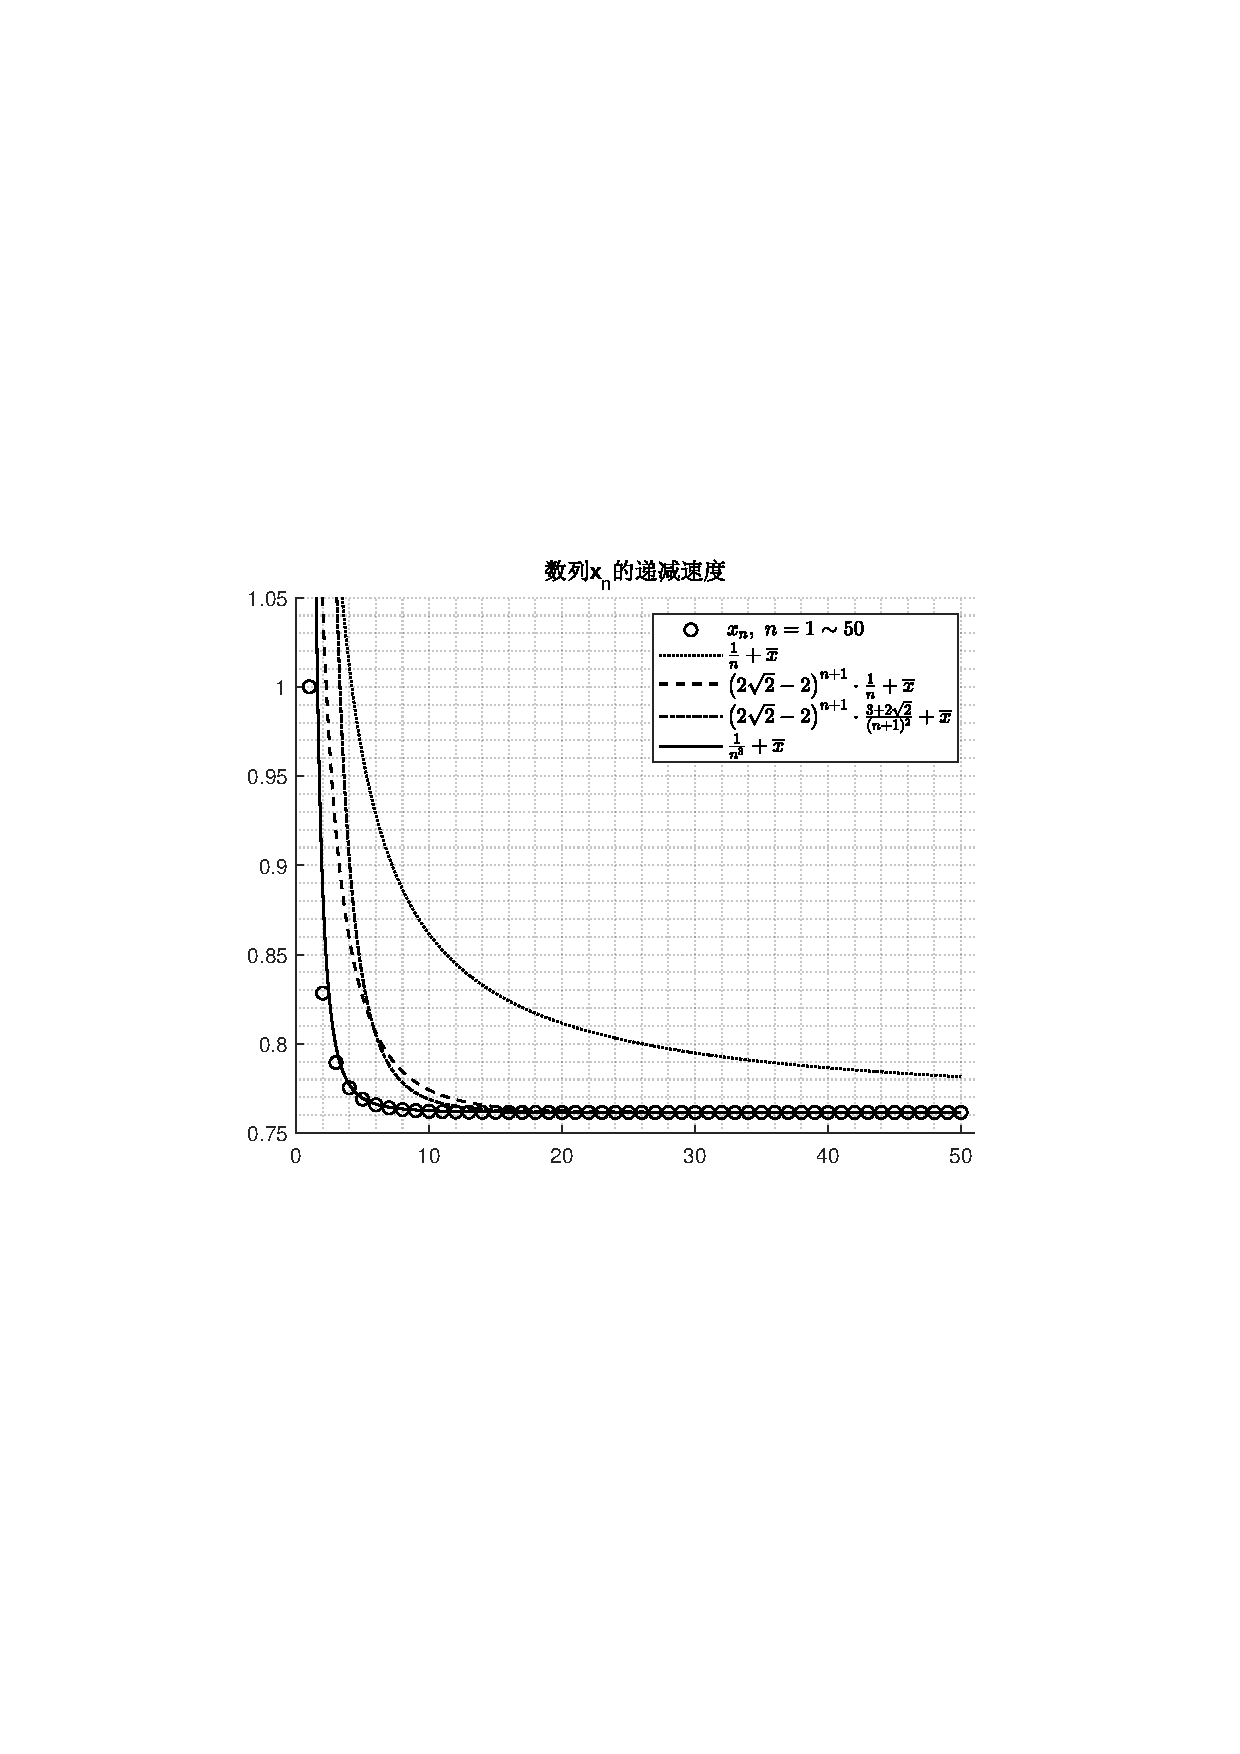
\includegraphics[width=0.6\linewidth]{2013安徽高考dilog实根递减速度}
\end{figure} \\
\textbf{注3}:当$ n $是偶数时,$ f_n(x)=0 $有两个实根,一个实根位于区间$ \left(\dfrac{3}{4},1\right) $内,这个实根随着$ n $的增加而单调递减,极限是
$ \overline{x}=0.761542\cdots $;
另一个实根位于区间$ (-5,-1) $内,这个实根随着$ n $的增加而单调递增,
极限是$ -1.027\cdots $. 极小值点是唯一的,且横坐标一定位于区间$ [-2,0) $内,
随$ n $的增加而递增,极小值始终大于等于$ f_4(x) $的极小值$ -2.005826\cdots $. 
当$ n $是奇数时,$ f_n(x) $在\textbf{R}上单调递增,$ f_n(x)=0 $有且仅有一个实根。

先证明$ f_n(-1)<0 $,(\ref{安徽f2k_1<0})、(\ref{安徽f2k+1_1<0})
式每个中括号内都是负数,
\begin{align}
  f_{2k}(-1) =-1+\left[-1+\dfrac{1}{2^2}\right]+\left[-\dfrac{1}{3^2}
    +\dfrac{1}{4^2}\right] +\cdots+\left[-\dfrac{1}{(2k-1)^2}
    +\dfrac{1}{(2k)^2}\right]<0 \label{安徽f2k_1<0}  
\end{align}
\begin{align}
    &\ f_{2k+1}(-1) \nonumber \\
   =&\ -1+\left[-1+\dfrac{1}{2^2}\right]+\left[-\dfrac{1}{3^2}
    +\dfrac{1}{4^2}\right]+\cdots+\left[-\dfrac{1}{(2k-1)^2}
    +\dfrac{1}{(2k)^2}\right]-\dfrac{1}{(2k+1)^2}<0 
    \label{安徽f2k+1_1<0} 
\end{align}

再证明$ f_{2k}(-5)>0 $,
\begin{align}
     &\ f_{2k}(-5) \nonumber \\
    =&\ -1+\left[-5+\dfrac{5^2}{2^2}\right]+\left[-\dfrac{5^3}{3^2}
    +\dfrac{5^4}{4^2}\right] +\cdots+\left[-\dfrac{5^{2k-1}}{(2k-1)^2}
    +\dfrac{5^{2k}}{(2k)^2}\right] \nonumber \\
    =&\ \underbrace{-1+5\left[-1+\dfrac{5}{2^2}\right]}_{>0}
    +\dfrac{5^3}{3^2}\left[
    -1+\dfrac{5\cdot 3^2}{4^2}\right]+\cdots+\dfrac{5^{2k-1}}
    {(2k-1)^2}\left[-1+\dfrac{5\cdot (2k-1)^2}{(2k)^2}\right]>0
    \label{安徽f2k_5>0}
\end{align}
因为$ \dfrac{5\cdot (2k-1)^2}{(2k)^2}=5\left(1-\dfrac{1}{2k}\right)^2 $
在$ k\in[1,+\infty) $时单调递增,所以$ -1+\dfrac{5\cdot (2k-1)^2}
{(2k)^2}>0 $在$ k\in[1,+\infty) $时恒成立,(\ref{安徽f2k_5>0})式的每个
中括号内都为正数,$ f_{2k}(-5)>0 $成立。

还可以研究如何使用迭代法解方程。

$f_n(x),\ n=2,3,\cdots, 12 $的图像如下:
\begin{figure}[h]
    \centering
    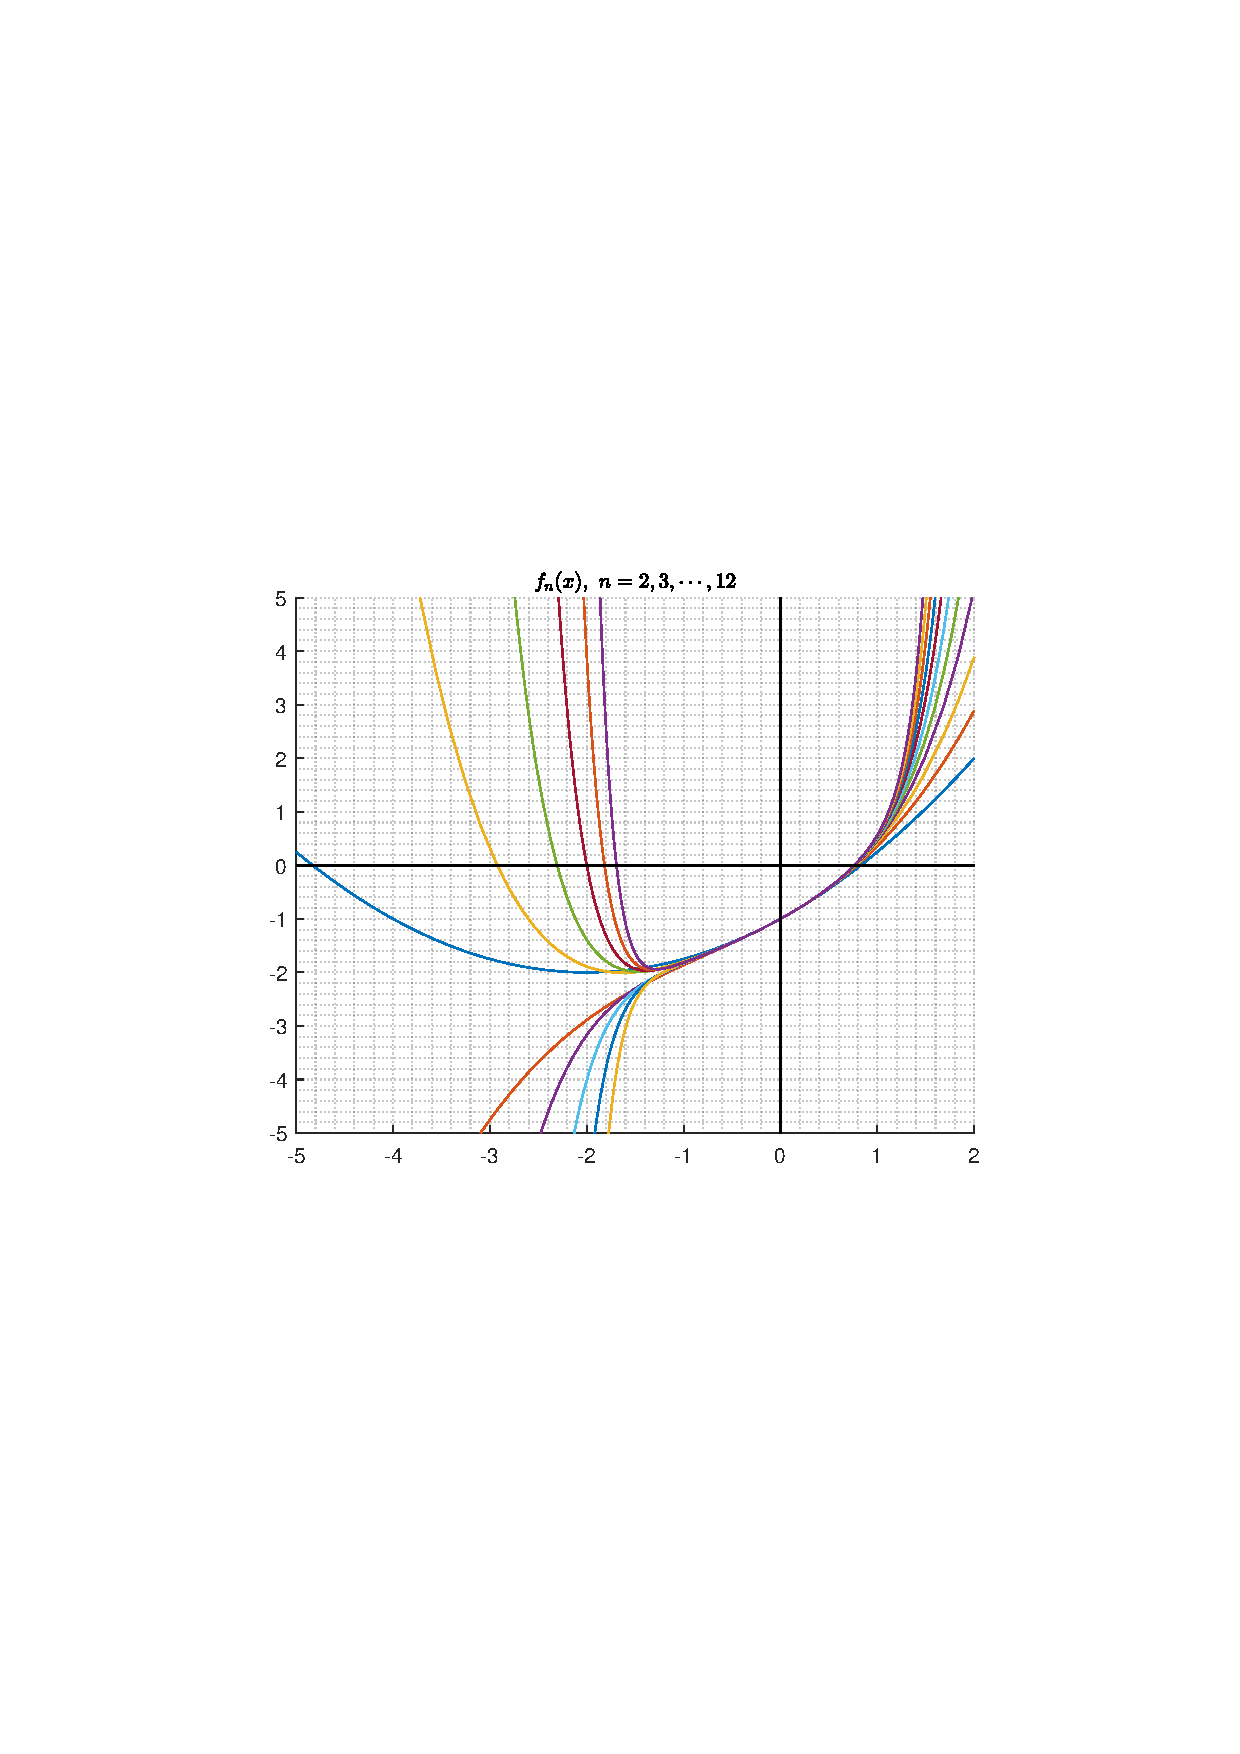
\includegraphics[width=0.6\linewidth]{2013安徽高考dilog截断多项式图像}
\end{figure}

$ f_n(x),\ n=10,30,,50,70,90 $的全部复数根的分布如下图:
\begin{figure}[h]
    \centering
    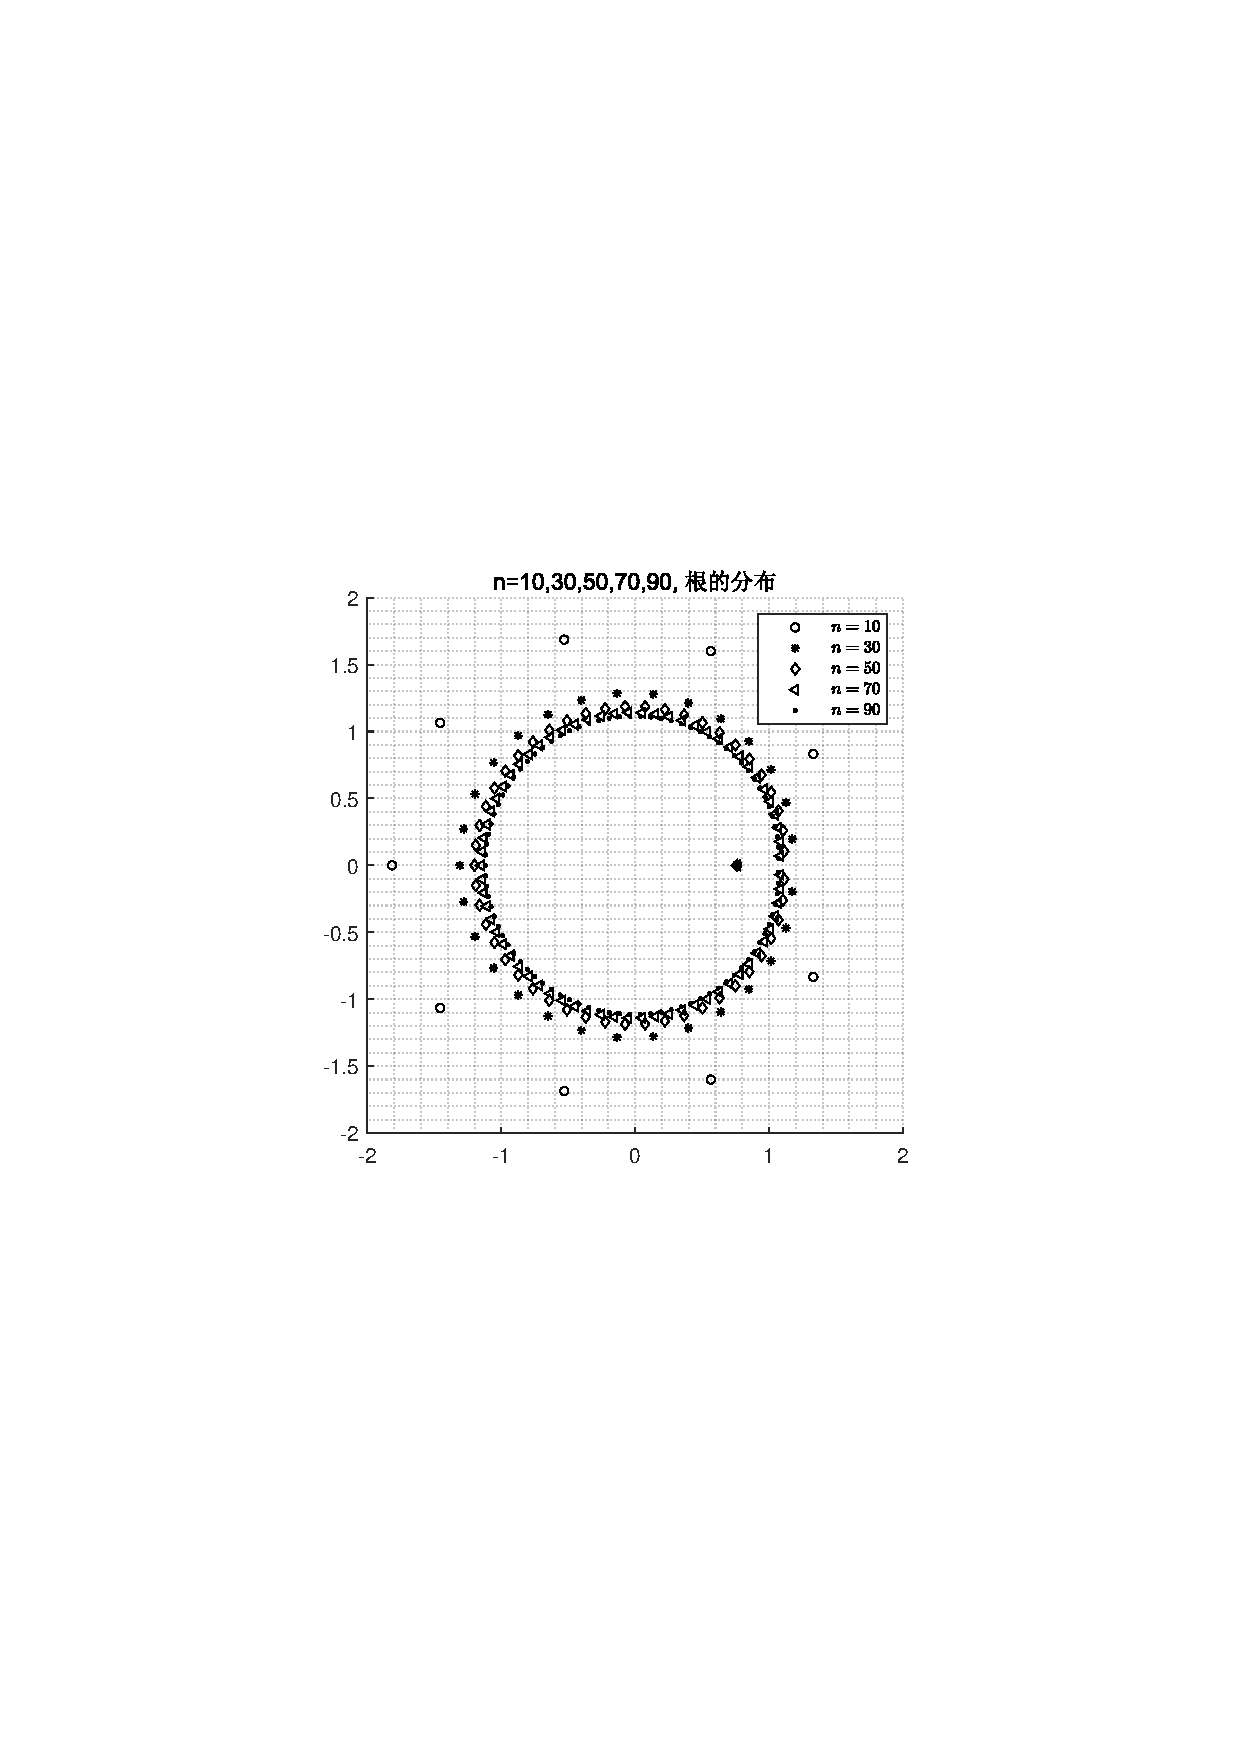
\includegraphics[width=0.6\linewidth]{2013安徽高考dilog截断根的分布10-30-50}
\end{figure} \\
可以看出,对于某个$ n $,全部复数根近似分布在一个椭圆上,随着$ n $增加,椭圆在缩小,但不会变成无限小,而是存在一个极限椭圆。绘制上图的MATLAB代码如下:
\lstset{
    backgroundcolor = \color{gray!5},    % 背景色:灰色
    basicstyle = \small\ttfamily,           % 基本样式 + 小号字体
    rulesepcolor= \color{black},             % 代码块边框颜色
    breaklines = true,                  % 代码过长则换行
    %	numbers = left,                     % 行号在左侧显示
    numberstyle = \small,               % 行号字体
    keywordstyle = \color{blue},            % 关键字颜色
    commentstyle =\color{black!100},        % 注释颜色
    stringstyle = \color{red!100},          % 字符串颜色
    frame = single,                  % 用方框框住代码块
    showspaces = false,                 % 不显示空格
    columns = fixed,                    % 字间距固定
    language=matlab
}
\begin{lstlisting}
    clc;  close all;
    syms x; 
    N=200;
    an=(1:N).^(-2);  % an代表fn(x)的系数,但不包含常数项-1
    z=zeros(N,N);
    for k=1:N
    z(k,1:k)=roots([fliplr(an(1:k)),-1]);  % 求多项式的全部根
    end
    figure 
    hold on
    axis equal
    plot(z(10,1:10),'ko','markersize',4)
    plot(z(30,1:30),'k*','markersize',4)
    plot(z(50,1:50),'kd','markersize',4)
    plot(z(70,1:70),'k<','markersize',4)
    plot(z(90,1:90),'k.')
    axis([-2 2 -2 2])
    grid minor
    legend('$n=10$','$n=30$','$n=50$','$n=70$','$n=90$', ...
    'interpreter','latex','fontsize',8)
\end{lstlisting} 
而$ n=2,3,4,\cdots,100 $时,
全部根的分布情况如下图,似乎是落在某些规则的曲线上,相当有趣。
\begin{figure}[H]
    \centering
    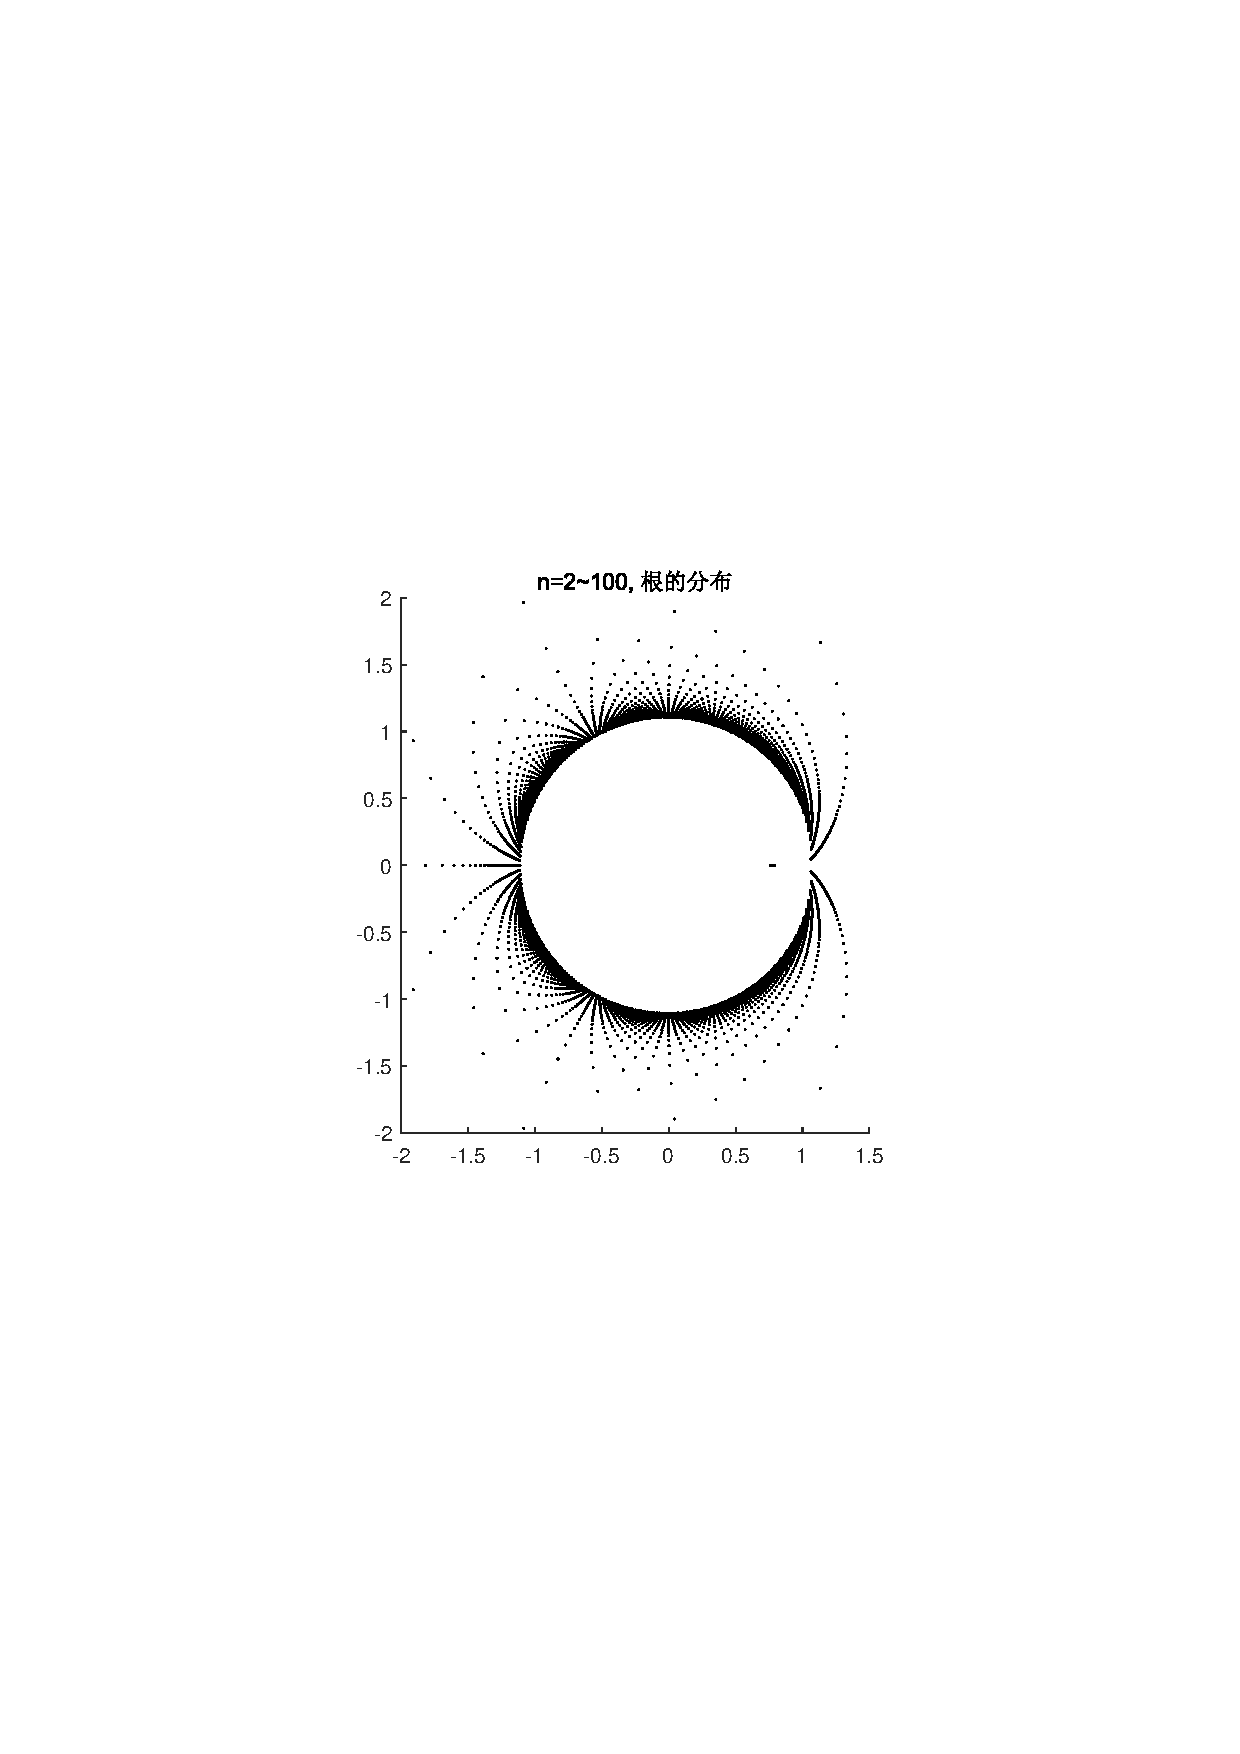
\includegraphics[width=0.6\linewidth]{2013安徽高考dilog截断根的分布2_100}
\end{figure} 

\noindent \textbf{注4}$ ^* $:对于$ \mathrm{Li}_2(x) $,还有如下性质\footnote{
$ \diamond $ https://www.maths.lancs.ac.uk/$ \sim $jameson/dilog.pdf \\
$ \diamond $ https://people.mpim-bonn.mpg.de/zagier/files/doi/10.1007/
978-3-540-30308-4\_1/fulltext.pdf },
\begin{gather*}
\mathrm{Li}_2(x)+\mathrm{Li}_2(-x)=\dfrac{1}{2}\mathrm{Li}_2(x^2) \\
\mathrm{Li}_2(-1)=-\dfrac{1}{2}\mathrm{Li}_2(1)=-\dfrac{1}{2}\zeta(2)=
-\dfrac{\pi^2}{12} \quad (\text{上式中令}\ x=1) \\
\int_0^1 \mathrm{Li}_2(x) \d x=\zeta(2)-1=\dfrac{\pi^2}{6}-1 \\
\mathrm{Li}_2(x)+\mathrm{Li}_2(1-x)=\zeta(2)-\ln x\ln(1-x) 
\quad (\text{欧拉反射公式}) \\
\mathrm{Li}_2\left(\dfrac{1}{2}\right)=\dfrac{1}{2}\left[\zeta(2)-
(\ln 2)^2\right]=\dfrac{\pi^2}{12}-\dfrac{1}{2}(\ln 2)^2 \quad 
(\text{上式中令}\ x=\dfrac{1}{2})  \\
\mathrm{Li}_2(-x)+\mathrm{Li}_2\left(-\dfrac{1}{x}\right)=-\zeta(2)-
\dfrac{1}{2}(\ln x)^2 \\
\mathrm{Li}_2(1-x)+\mathrm{Li}_2\left(1-\dfrac{1}{x}\right)=
-\dfrac{1}{2}(\ln x)^2   
\end{gather*}
下面给出欧拉反射公式的证明,
\begin{align*}
    \mathrm{Li}_2(x)=-\int_0^x \dfrac{\ln(1-u)}{u} \d u=&\ \underbrace{
        -\left.\left[\ln u\ln(1-u) \right]\right |_0^x-\int_0^x 
        \dfrac{\ln u}{1-u} \d u}_{\text{分部积分}} \\
    =&\ -\ln x\ln(1-x) -\int_0^1 \dfrac{\ln u}{1-u} \d u+\int_x^1 
    \dfrac{\ln u}{1-u} \d u \\
    =&\ -\ln x\ln(1-x)+\zeta(2)-\mathrm{Li}_2(1-x)
\end{align*}
上面还利用了$ \displaystyle{\lim_{u\to 0}[\ln u\ln(1-u)]}=0 $. 

% ResearchOnTheLawOfHigherOrderDerivatives.m
\item $ ^* $\ $ n \in\textbf{N}^+ $,计算$ \e^{-x^2}, \dfrac{\e^x}{x},
x^ne^x,(x^2-1)^n $的高阶导数,观察规律,尝试用数学归纳法证明。\\
\textbf{解}\ 
$ \e^{-x^2} $的$ n $阶导数乘上$ \dfrac{(-1)^n\e^{x^2}}{2^n} $后得到的多项式如下:
\begin{align*}
    & x \\
    & x^2 -\dfrac{1}{2} \\
    & x^3 -\dfrac{3}{2}x \\
    & x^4 - 3x^2 + \dfrac{3}{4} \\
    & x^5 - 5x^3 + \dfrac{15}{4}x \\
    & x^6 -\dfrac{15}{2}x^4 + \dfrac{45}{4}x^2 - \dfrac{15}{8} \\
    & \cdots \\
    & x^n-\dfrac{n(n-1)}{4}x^{n-2}+\dfrac{n(n-1)(n-2)(n-3)}{32}x^{n-4}-\cdots 
\end{align*}
$ \dfrac{\e^x}{x} $的$ n $阶导数设为$ f_n(x) $,
则$ x^{n+1}\e^{-x}f_n(x) $为$ n $次多项式,如下:
\begin{align}
    & x-1    \label{ex_x导数多项式1}         \\
    & x^2-2x+2                              \\
    & x^3-3x^2+6x-6                         \\
    & x^4-4x^3+12x^2-24x+24                 \\
    & x^5-5x^4+20x^3-60x^2+120x-120         \\
    & x^6-6x^5+30x^4-120x^3+360x^2-720x+720  \\
    & \cdots  \nonumber \\
    & x^n-nx^{n-1}+n(n-1)x^{n-2}-n(n-1)(n-2)x^{n-3}+\cdots
    \label{ex_x导数多项式7}
\end{align}
用数学归纳法容易证明以下结果:
\begin{gather}
    nf_{n-1}(x)+xf_n(x)=\e^x \\
    n[x^{n}\e^{-x}f_{n-1}(x)]+[x^{n+1}\e^{-x}f_n(x)]=x^n 
    \label{ex_x导数多项式递推关系} 
\end{gather}
(\ref{ex_x导数多项式递推关系})式就是多项式(\ref{ex_x导数多项式1})
$ \sim $(\ref{ex_x导数多项式7})的递推关系。\\
$ x^5\e^x $的$ 1\sim 5 $阶导数乘上$ \e^{-x} $后得到的多项式如下:
\begin{align*}
    & x^4+4x^3                  \\
    & x^4+8x^3+12x^2            \\
    & x^4+12x^3+36x^2+24x       \\
    & x^4+16x^3+72x^2+96x+24    \\
    & x^4+20x^3+120x^2+240x+120 
\end{align*}
$ \dfrac{1}{2^n n!}\left[(x^2-1)^n\right]^{(n)} $结果如下\footnote{
    这些多项式被称为勒让德(Legendre)多项式,参见《 特殊函数概论》 第210页,
    $ P_n(x) $的生成函数.微商表示——罗巨格(Rodrigues)公式。} :
\begin{align*}
    & x                                    \\
    & \dfrac{1}{2}(3x^2-1)                  \\
    & \dfrac{1}{2}(5x^3-3x)                 \\
    & \dfrac{1}{8}(35x^4-30x^2+3)           \\
    & \dfrac{1}{8}(63x^5-70x^3+15x)         \\
    & \dfrac{1}{16}(231x^6-315x^4+105x^2-5) 
\end{align*} 

\item (2014,江苏高考)已知函数$f_{0}(x)=\dfrac{\sin x}{x}\ (x\neq 0)$,
设$f_{n}(x)$为$f_{n-1}(x)$的导数,$n\in \textbf{N}^{+}$. \\
(1)求$ \left|2f_{1}\Big(\dfrac{\pi}{2}\Big)+
\dfrac{\pi}{2}f_{2}\Big(\dfrac{\pi}{2}\Big)\right| $的值;\\
(2)证明:对任意的$n\in \textbf{N}^{+}$,等式$\left|nf_{n-1}
\Big(\dfrac{\pi}{4}\Big)+\dfrac{\pi}{4}f_{n}
\Big(\dfrac{\pi}{4}\Big)\right|=\dfrac{\sqrt{2}}{2}$成立。\\
\textbf{解}\ (1) $ -1 $. \\
(2) $ xf_0(x)=\sin x $,两边对$ x $求导:$ f_0(x)+xf_1(x)=\cos x=
\sin\Big(x+\dfrac{\pi}{2}\Big) $,
两边再对$ x $求导:$ f_1(x)+f_1(x)+xf_2(x)=-\sin x=
\sin\Big(x+\dfrac{2\pi}{2}\Big) $,大胆猜测
\begin{gather}\label{sinx_x高阶导数递推关系}
    nf_{n-1}(x)+xf_{n}(x)=\sin\Big(x+\dfrac{n\pi}{2}\Big)
\end{gather}
用数学归纳法证明,当$ n=1 $时显然成立,
假设(\ref{sinx_x高阶导数递推关系})式对$ n $成立,(\ref{sinx_x高阶导数递推关系})
式两边对$ x $求导,有
\begin{gather*}
    nf_{n}(x)+f_n(x)+xf_{n+1}(x)=\cos\Big(x+\dfrac{n\pi}{2}\Big) \\
    (n+1)f_n(x)+xf_{n+1}(x)=\sin\Big(x+\dfrac{(n+1)\pi}{2}\Big)
\end{gather*}
即$ n $换成$ n+1 $也成立,(\ref{sinx_x高阶导数递推关系})式得证。
所以,
\begin{gather*}
    \left|nf_{n-1}\Big(\dfrac{\pi}{4}\Big)+\dfrac{\pi}{4}f_{n}
    \Big(\dfrac{\pi}{4}\Big)\right|=\left|\sin\Big(\dfrac{\pi}{4}
    +\dfrac{n\pi}{2}\Big)\right|=\dfrac{\sqrt{2}}{2}
\end{gather*}
\textbf{注}:
\begin{align*}
    f_1(x) &=\dfrac{x\cos x-\sin x}{x^2}  \\
    f_2(x) &=\dfrac{-x^{2}\sin x-2x\cos x+2\sin x}{x^3}  \\
    f_3(x) &=\dfrac{-x^{3}\cos x+3x^{2}\sin x+6x\cos x-6\sin x}{x^4}  \\
    f_4(x) &=\dfrac{x^{4}\sin x+4x^{3}\cos x-12x^{2}\sin x-24x\cos x+
        24\sin x}{x^5}
\end{align*}
可猜测,
\begin{align*}
    f_n(x) &=\dfrac{1}{x^{n+1}}\Bigg[x^{n}\sin \Big(x+\dfrac{n\pi}{2}\Big)+
    nx^{n-1}\sin \Big(x+\dfrac{(n+1)\pi}{2}\Big)  \\
    & + n(n-1)x^{n-2}\sin \Big(x+\dfrac{(n+2)\pi}{2}\Big)
    +n(n-1)(n-2)x^{n-3}\sin \Big(x+\dfrac{(n+3)\pi}{2}\Big)  \\
    & +\cdots +n!\,\sin\Big(x+\dfrac{(2n-1)\pi}{2}\Big)+
    n!\,\sin(x+n\pi)\Bigg]
\end{align*}
利用数学归纳法可证明上式(略)。$ \dfrac{\sin x}{x} $与$ \dfrac{\e^x}{x} $
的高阶导数的系数的规律是一致的,请读者利用欧拉公式$ \e^{\i x}=\cos x+\i\sin x $
进行思考。

\item$^*$ 设$ \zeta(s) $代表黎曼zeta函数,已知如下4个等式:\\
$(1) \q \zeta(s)=2^s\pi^{s-1}\sin\left(\dfrac{\pi s}{2}\right)\Gamma(1-s)
\zeta(1-s) $, \\
$(2)\q \Gamma(s+1)=s\Gamma(s) $, \\
$(3) \q \Gamma\left(\dfrac{s}{2}\right)
\Gamma\left(1-\dfrac{s}{2}\right)=
\dfrac{\pi}{\sin\left(\frac{\pi s}{2}\right)} $, \\
$(4) \q \Gamma(s)=\dfrac{2^{s-1}}{\sqrt{\pi}}
\Gamma\left(\dfrac{s+1}{2}\right) \Gamma\left(\dfrac{s}{2}\right) $, \\
记$\xi(s)=\Gamma\left(\dfrac{s}{2}+1\right)(s-1)\pi^{-s/2}\zeta(s) $,求证:
$ \xi(s)=\xi(1-s) $. \\
\textbf{证}\ 利用(1)和(2)式,
\begin{align*}
    \xi(s) &=\dotuline{\Gamma\left(\dfrac{s}{2}+1\right)}(s-1)\pi^{-s/2}
    \underline{\zeta(s)} \\
    & = \dotuline{\dfrac{s}{2}\Gamma\left(\dfrac{s}{2}\right)}(s-1)\pi^{-s/2}
    \underline{2^s\pi^{s-1}\sin\left(\dfrac{\pi s}{2}\right)\Gamma(1-s)
        \zeta(1-s)}  \\
    & = 2^{s-1}s(s-1)\pi^{s/2-1}\sin\left(\dfrac{\pi s}{2}\right)
    \Gamma\left(\dfrac{s}{2}\right)\Gamma(1-s)\zeta(1-s)\q\q\q (5)
\end{align*}
把(4)式中的$ s $换成$ 1-s $,有$ \Gamma(1-s)=\dfrac{2^{-s}}{\sqrt{\pi}}
\Gamma\left(1-\dfrac{s}{2}\right)\Gamma\left(\dfrac{1-s}{2}\right) $,
代入(5)式:
\begin{align*}
    \xi(s) &=  2^{s-1}s(s-1)\pi^{s/2-1}\sin\left(\dfrac{\pi s}{2}\right)
    \Gamma\left(\dfrac{s}{2}\right)\dashuline{
        \dfrac{2^{-s}}{\sqrt{\pi}}\Gamma\left(1-\dfrac{s}{2}\right)
        \Gamma\left(\dfrac{1-s}{2}\right) }\zeta(1-s) \\
    & =2^{-1}s(s-1) \pi^{s/2-3/2} \uwave{\sin\left(\dfrac{\pi s}{2}\right)
        \Gamma\left(\dfrac{s}{2}\right)\Gamma\left(1-\dfrac{s}{2}\right)}
    \Gamma\left(\dfrac{1-s}{2}\right)\zeta(1-s)\q (\text{利用(3)式}) \\
    & =2^{-1}s(s-1) \pi^{s/2-3/2} \uwave{\pi} 
    \Gamma\left(\dfrac{1-s}{2}\right)\zeta(1-s) \\
    &= (-s)\dotuline{\left(\dfrac{1-s}{2}\right) \Gamma\left(\dfrac{1-s}{2}\right)}
    \pi^{-(1-s)/2}\zeta(1-s)\q (\text{利用(2)式})\\
    &= \dotuline{\Gamma\left(\dfrac{1-s}{2}+1\right)}
    [(1-s)-1]\pi^{-(1-s)/2}\zeta(1-s)=\xi(1-s)
\end{align*}
\\
有能力的读者还可以自学微分方程方面的内容,对理解高中物理的某些运动学问题有帮助,
比如两个质量块之间用一根弹簧连接,它们一起在一个光滑表面上运动,这两者的速度-时间函数分别是怎样的。
匀强磁场中有两根导轨,一根光滑的导体棒沿着导轨滚动切割磁感线,另外一端串联一个电阻消耗电能,
滚动棒的速度-时间函数是怎样的。雨滴从高空落下,空气阻力与速度成正比,雨滴的运动规律又是怎样的。

\end{enumerate}
%~\newpage

\section{习题} 
\begin{enumerate}[label={\textbf{\arabic*.}},leftmargin=
    \inteval{\myenumleftmargin}pt]
\item 对以下函数,分别计算$ (fg)' $和$ f'g' $,判断两者是否相等。\\
(1)$ f(x)=\e^{x^2},\ g(x)=\sqrt{2x-1}\e^x $.\\
(2)$ f(x)=\e^{x+x^2/2},\ g(x)=x\e^x $. \\
(3)$ f(x)=x^n,\ g(x)=\dfrac{1}{(n-x)^n} $,其中,$ n\in \textbf{N}^+ $.

\item 手工分别绘制$ y=(x-2)^k(x-4),\ k=2,3,4 $的函数图像,然后用GeoGebra验证。

\item 证明,对任意实数$ x $,都有$ 3x^4+6x^3-3x+1\geq \dfrac{1}{4} $.
(这个4次多项式来源于$ \sum\limits_{l=1}^{n} l^6=
\dfrac{1}{42}n(n+1)(2n+1)(3n^4+6n^3-3n+1) $\ ). 
请分别使用求导法和配方法。

\item 求$ f(x)=\sqrt{x^2+9}+\sqrt{x^2-4x+20} $的最小值。

\item 
(1) 设$ 0<x_1<1<x_2 $,且$ (\ln x_1)^2=(\ln x_2)^2 $,
求证:$ x_1+x_2>2 $. \\
(2) 求证:当$x>0$时,$ x+\dfrac{1}{x}-2\geq (\ln x)^2 $. 

\item 求证:当$ x<\dfrac{1}{2} $时,$ \e^x\leq \dfrac{1}{(1-\dfrac{x}{2})^2}
\leq \dfrac{1}{1-x}\leq \sqrt{\dfrac{1}{1-2x}} $.(均为$ \e^x\geq 1+x $的衍生不等式。)

\item $ f(x)=\e^x-\dfrac{1}{2}x^2 $,求证:$ f(x)+f(-x)\geq 2 $. 

\item (2021,高考全国乙卷)设$a=2\ln1.01,\ b=\ln1.02,\ c=\sqrt{1.04}-1 $,则(\ \ ) \\
A.\ $a<b<c$\q\q B.\ $b<c<a$ \q\q C.\ $b<a<c$ \q\q D.\ $c<a<b$ 

\item 求$ y=f(x)=\dfrac{x+1}{x^2+1} $的切线在$ y $轴上的截距的范围。

\item 已知$ p>0,q>0,\ p+q=1$. \\
(1) $f(x)=\sqrt{x} $,求证:$ pf(x_1)+qf(x_2)\leq f(px_1+qx_2) $. \\
(2) $f(x)=x^2 $,求证:$ pf(x_1)+qf(x_2)\geq f(px_1+qx_2) $. \\
(3) $f(x)=x^3 $,$ x_1>0,\ x_2>0 $,
求证:$ pf(x_1)+qf(x_2)\geq f(px_1+qx_2) $. \\
(4) $f(x)=\ln x $,求证:$ pf(x_1)+qf(x_2)\leq f(px_1+qx_2) $. \\
(5) $f(x)=\e^x $,求证:$ pf(x_1)+qf(x_2)\geq f(px_1+qx_2) $. \\
(6) $f(x)=\sqrt{x^2+2} $,求证:$ \dfrac{1}{2}[f(x_1)+f(x_2)]\geq 
f\Big(\dfrac{x_1+x_2}{2}\Big) $. \\
(7) $f(x)=x\ln x $,求证:$ \dfrac{1}{2}[f(x_1)+f(x_2)]\geq 
f\Big(\dfrac{x_1+x_2}{2}\Big) $. \\
(8) $f(x)=x\e^x $,求证:$ \dfrac{1}{2}[f(x_1)+f(x_2)]\geq 
f\Big(\dfrac{x_1+x_2}{2}\Big) $. 

\item 设$ r>1 $,求证:$ \sum\limits_{l=1}^n l^r>\dfrac{n^{r+1}}{r+1}+\dfrac{1}{2}n^r $.
(提示:令$ f(x)=x^r $,利用(\ref{Hermite-Hadamard不等式1})式) 

\item (I)求证:任意$ x\geq 1 $,有$ 2x-\dfrac{1}{x}-1\geq 3\ln x $.\\
(II) 当$ x\geq 1 $时,$ 5x-\dfrac{3}{x}-2\geq K\ln x $恒成立,求$ K $的最大值。

\item (2015,北京高考,理)已知函数$ f(x)=\ln\dfrac{1+x}{1-x} $.\\
(1)求曲线$ y=f(x) $在点$ (0,f(0)) $处的切线方程;\\
(2)求证:当$ x\in(0,1) $时,$ f(x)>2\left(x+\dfrac{x^{3}}{3}\right) $;\\
(3)设实数$ k $使得 $ f(x)>k\left(x+\dfrac{x^{3}}{3}\right) $
对$ x\in(0,1) $恒成立,求$ k $的最大值。

\item 
(2019,全国II卷)已知函数$ f(x)=\ln x-\dfrac{x+1}{x-1} $,\\
(1)讨论$ f(x) $的单调性,并证明$ f(x) $有且仅有两个零点;\\
(2)设$ x_0 $是$ f(x) $的一个零点,证明:曲线$ y=\ln x $在点$ A(x_0,\ln x_0) $
处的切线也是曲线$ y=\e^x $的切线。

\item 已知函数$f(x)=\dfrac{\e^x-\e^{-x}}{4}-x\ (x>0) $和
$ g(x)=x-\ln(2x+\sqrt{4x^2+1})\ (x>0) $. \\
(1) 讨论$ f(x) $和$ g(x) $的单调性;\\
(2) 证明:存在直线$y=\pm b$,其与两条曲线$y=f(x)$和$y=g(x)$共有三个不同的交点,
并且从左到右的三个交点的横坐标成等差数列。

\item 求$ 17^{3/2}+18^{3/2}+19^{3/2}+\cdots + 49^{3/2} $的整数部分。

\item 求$ \sum\limits_{k=1}^n k(k+1)(k+2) $.

\item $ ^* $ 求$ \e^{1/x} $的$ n $阶导数乘上
$ \dfrac{(-1)^nx^{2n}\e^{-1/x}}{n!} $的结果。

\item 求证:$ \forall n\in \textbf{N}^+ $,$ \sum\limits_{k=1}^{n} 
\e^{\frac{1}{k}}\leq n+\ln n+\e -1 $. 

\item 定义函数$ f(x)=a\ln x+x+\e^{-x} \ (a<0) $. \\
(I)当$ a=-1 $时,判断$ f(x) $有无极值,并说明理由;\\
(II)若$ f(x)\geq x^a $对任意$ x>1 $恒成立,求$ a $的最小值。

\item (2015,湖北高考) 数列$ \{a_n\} $的各项均为正数,$ b_n=n\left(1+\dfrac{1}{n}\right)^na_n $,$ \e $为自然对数的底数。\\
(1)求函数$ f(x)=1+x-\e^{-x} $的单调区间,并比较$ \left(1+\dfrac{1}{n}\right)^n $与
$ \e $的大小;\\
(2)求$ \dfrac{b_1b_2\cdots b_n}{a_1a_2\cdots a_n} $的表达式;\\
(3)令$ c_n=(a_1a_2\cdots a_n)^{1/n} $,数列$ \{a_n\},\{c_n\} $的前$ n $项和分别是
$ S_n,T_n $,证明:$ T_n<eS_n $.

\item (2013,湖南高考,文科)已知函数$ f(x)=\dfrac{1-x}{1+x^2}\e^x $.\\
(I)求$ f(x) $的单调区间;\\
(II)证明:若$ f(x_1)=f(x_2)\ (x_1\neq x_2) $,则$ x_1+x_2<0 $. 

\item (2011,辽宁高考)已知函数$ f(x)=\ln x-ax^2+(2-a)x $.\\
(I)讨论$ f(x) $的单调性;\\
(II)设$ a>0 $,证明:若$ 0<x<\dfrac{1}{a} $,则
$ f\left(\dfrac{1}{a}+x\right)>f\left(\dfrac{1}{a}-x\right) $;\\
(III)若函数$ y=f(x) $的图象与$ x $轴交于$ A,B $两点,线段$ AB $中点的横坐标为$ x_0 $,证明:$ f'(x_0)<0 $. 

% LiaoNing2013_Ode45.m
\item (2013,辽宁高考,理)已知函数$ f(x) $满足$ x^2f'(x)+2xf(x)=\dfrac{\e^x}{x},\ f(2)=\dfrac{\e^2}{8} $,则$ x>0 $时,$ f(x) $ \underline{\hspace{2cm}}. \\
A.有极大值,无极小值 \hspace{2cm}     B.有极小值,无极大值\\
C.既有极大值,又有极小值\hspace{1.4cm}  D.既无极大值,又无极小值

\item (2021,天津高考)已知$ a>0 $,函数$ f(x)=ax-x\e^x $.\\
(1)求曲线$ f(x) $在点$ (0,f(0)) $处的切线方程;\\
(2)证明函数$ f(x) $存在唯一的极值点;\\
(3)若$ \exists a $,使得$ f(x)\leq a+b $对任意的
$ x\in \textbf{R} $恒成立,求实数$ b $的取值范围。

\item (2022,南京大学强基计划)设$n>1$为正整数,证明:
\begin{align*}
    \Big(\dfrac{n+1}{3}\Big)^{n}<n!<\Big(\dfrac{n+1}{2}\Big)^{n}
\end{align*}

\item $ ^* $(微信公众号:数海漫游)已知函数$ f(x)=\ln x+a\left(\dfrac{5}{4x}+\dfrac{1}{4}\right),\ x>0 $.\\
(I)若$ a>0 $,当$ f(x) $的最小值为$ \dfrac{6}{5} $时,求$ a $的值。\\
(II)当$ 0<a<2-\sqrt{3} $时,$ f(x) $的两个零点记为$ x_1,x_2\ (x_1<x_2) $,求证:$ \sqrt{x_1^2+x_2^2+3}+a>2 $.

\item 设$ a>\e $,方程$ x\ln x=a $的根为$ x_0 $,求证:
$ \dfrac{a}{\ln a}<x_0\leq \dfrac{\e+1}{\e}\cdot \dfrac{a}{\ln a} $. \\
(提示:当$ r>1,\ x>1 $时,$ x^{1/r}\geq \dfrac{\e}{r}\ln x $.)

\item 求证:当 $ x\in \left(0,\dfrac{\pi}{2}\right) $时,
$ \cos x<1-\dfrac{4x^2}{\pi^2} $.

\item 求下列二元函数对$ x,y $的偏导数。\\
(1) $ z=\ln(x^2+y^2) $ \quad (2) $ z=\sqrt{x^2+y^2} $ \\
(3) $ z=x^4+6xy^3-y^5 $ \quad (4) $ z=\e^x\sin(x+y^2)  $ 

\item 设$ \i $是虚数单位,$ z=x+ y\i $,对于下面定义的$ u(x,y),\ v(x,y) $,
证明:$ \begin{cases}
    \dfrac{\partial u}{\partial x} =\dfrac{\partial v}{\partial y} \\
    \dfrac{\partial v}{\partial x} =-\dfrac{\partial u}{\partial y} 
\end{cases} $. \\
(1)\ $ \dfrac{1}{z}=\dfrac{1}{x+y\i}=\dfrac{x}{x^2+y^2}-\dfrac{y}{x^2+y^2}\i,
\ u(x,y)=\dfrac{x}{x^2+y^2},\ v(x,y)=-\dfrac{y}{x^2+y^2} $; \\
(2)\ $ \e^{z}=\e^{x+y\i}=\e^x(\cos y+\i\sin y),\ u(x,y)=\e^x \cos y,
\ v(x,y)=\e^x\sin y $; \\
(3)\ $ \sin z=\sin(x+y\i)=\sin x\cos(y\i)+\cos x\sin(y\i)=\sin x\cosh y+
\cos x\sinh y $, \\ $\ u(x,y)=\sin x\cosh y,\ v(x,y)=\cos x\sinh y $; \\
(注:$ (\sinh x)'=\cosh x,\ (\cosh x)'=\sinh x $). 

\item $ ^* $ 以下题目难度很大,高考不可能考,感兴趣的读者可借助软件研究。
\begin{enumerate}[label={(\arabic*)},itemsep=-1pt]
\item 已知$ a^a=b^b,\ 0<a<b<1 $,求证:$ a^{\ln 2}+b^{\ln2}>1 $. \\
\textbf{注}:函数$ y=x^x $的图像如下:
\begin{figure}[!htbp]
    \centering
    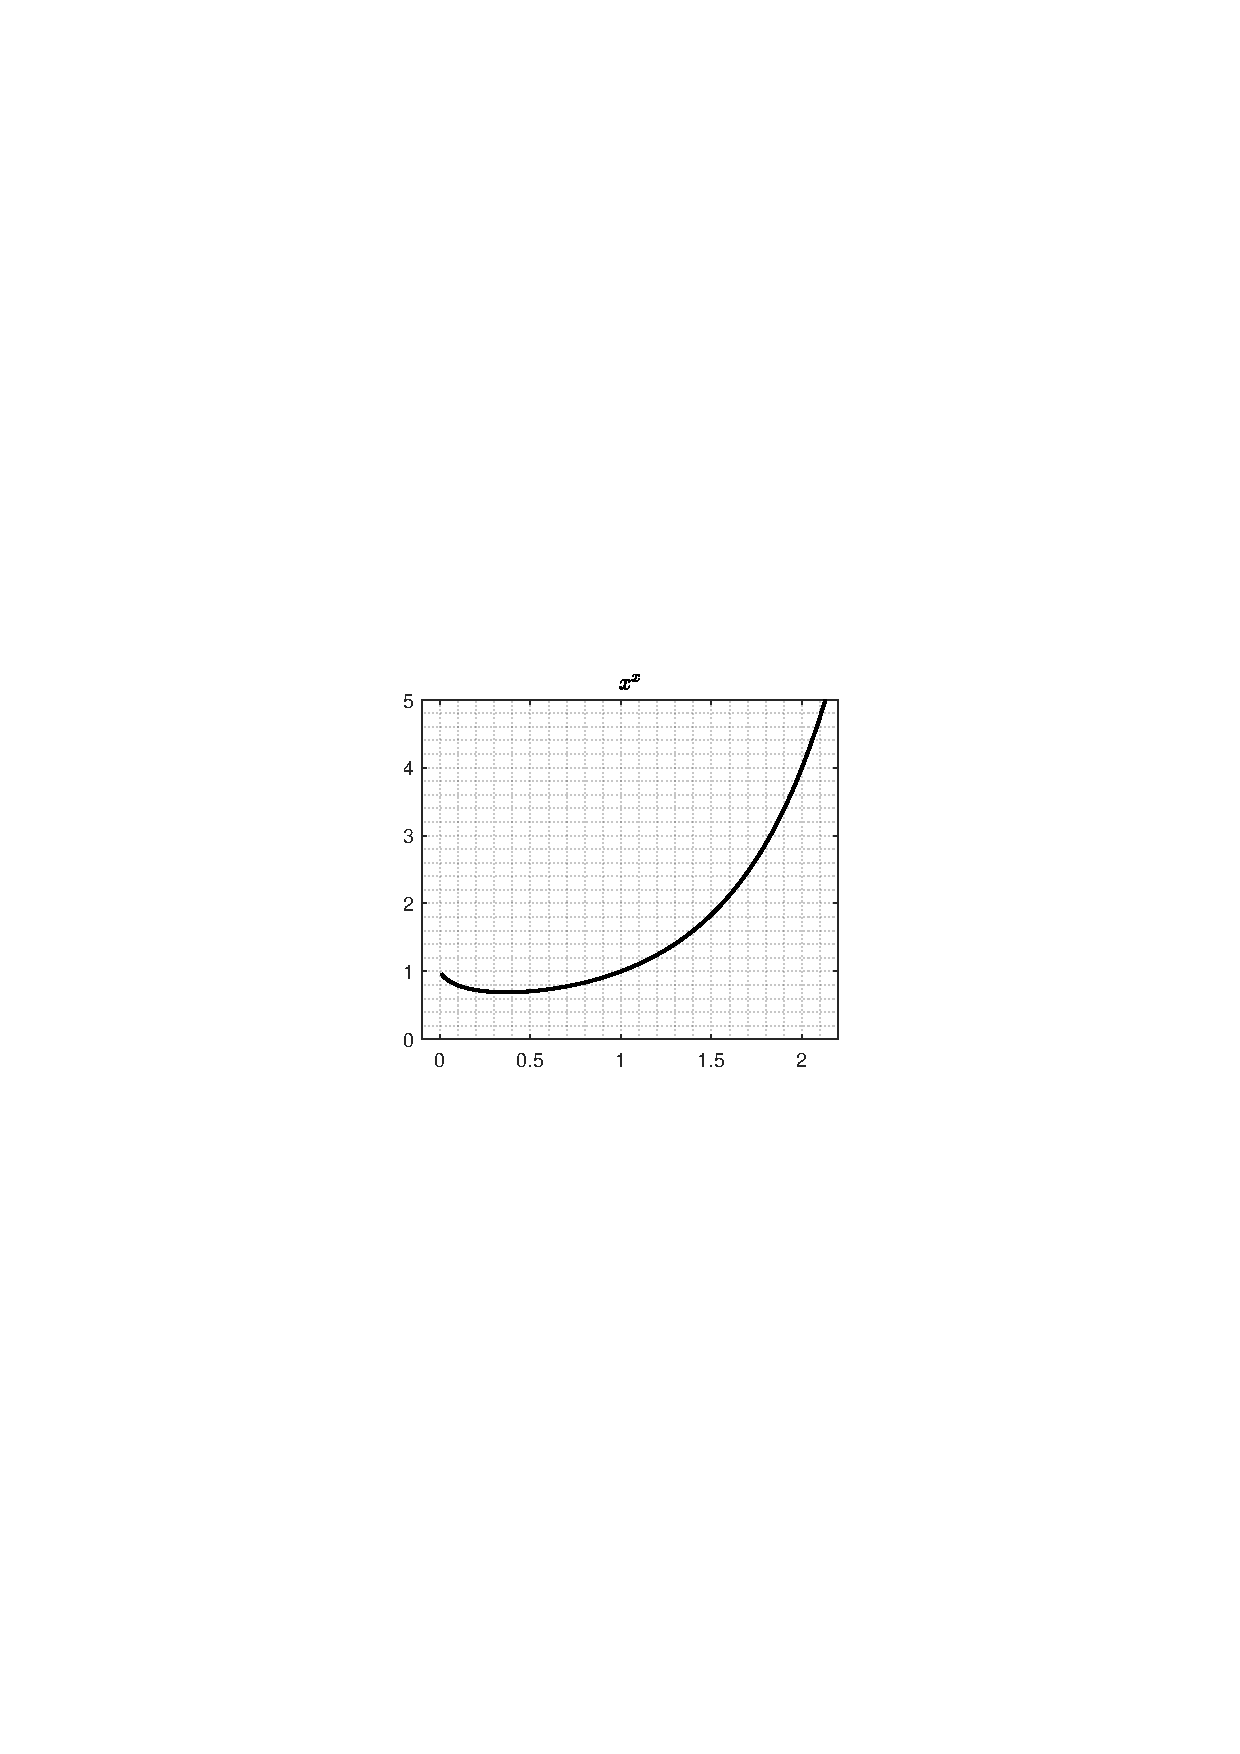
\includegraphics[width=0.4\linewidth]{幂指函数图像}
\end{figure} 
\item $ \dfrac{\ln x}{\ln(1-x)}>\left(\dfrac{1-x}{x}\right)^{
    \dfrac{1}{\ln 2}},\ x\in\left(\dfrac{1}{2},1\right) $. 
\item $ x^{\frac{1}{x}}\ln x<\sqrt{x},\ (x>0) $. (\textbf{注}:
$ x^{\frac{1}{x}}\ln x-\sqrt{x} $的极大值为$ -0.015439\cdots $) 
\item $ x^{\frac{1}{x}}\ln x >-\dfrac{2}{9},\ (x>0) $.(\textbf{注}:
$ x^{\frac{1}{x}}\ln x $的极小值为$ -0.222218\cdots $,与
$ -\dfrac{2}{9}=-0.222222\cdots $十分接近。) 
\item $ \left(\dfrac{\sin x}{x}\right)^3>\cos x,\ (0<|x|<4.7) $.
\item $ \sin\sqrt{\dfrac{2}{x}}>\sqrt{\dfrac{2}{x+1}},\ x>1.2 $.
\end{enumerate}


\end{enumerate}
\section{习题答案}
\begin{enumerate}[label={\textbf{\arabic*.}},leftmargin=
    \inteval{\myenumleftmargin}pt]
\item (1)$\ (fg)'=f'g'=\dfrac{4x^2\e^{x+x^2}}{\sqrt{2x-1}} $. \quad
(2)$\ (fg)'=f'g'=(1+x)^2\e^{2x+x^2/2} $. \\
(3)$\ (fg)'=f'g'=\dfrac{n^2x^{n-1}}{(n-x)^{n+1}} $. \\
\textbf{注}:$ (fg)'=f'g' $当然不可能对任意两个函数都成立,而是需要特意构造,此题的函数是通过求解微分方程找到的。

\item 略

\item $ f(x)=3x^4+6x^3-3x+1 $,$ f'(x)=12x^3+18x^2-3 $,
$ f''(x)=36x^2+36x=36x(x+1) $,
$ f''(x) $的对称轴是$ x=-\dfrac{1}{2} $,
$ f'(x) $的对称中心是$ \left(-\dfrac{1}{2},0\right) $,
恰好落在$ x $轴上,
那么$ f'(x) $必定可以写成$ 3\left(x+
\dfrac{1}{2}\right)(4x^2+ax-2) $,容易算出$ a=4 $,
所以,$ f'(x)=3\left(x+\dfrac{1}{2}\right)(4x^2+4x-2) $,
除了$ -\dfrac{1}{2} $,$ f'(x) $的另外两个零点是
$ -\dfrac{1\pm \sqrt{3}}{2} $. 
根据\ref{四次函数的轴对称性}的推广2,$ f(x) $的对称轴也是
$ x=-\dfrac{1}{2} $,$ f(x) $的形状像w,在
$ x=-\dfrac{1}{2} $处取得极大值$ \dfrac{31}{16} $;
在$ x=-\dfrac{1\pm \sqrt{3}}{2} $处取得极小值$ \dfrac{1}{4} $,
这说明$ f(x) $是没有实根的。配方法:设$ f(x)=3(x^2+bx+c)^2+d $,
展开后比较系数可得:$ f(x)=3\left(x^2+x-
\dfrac{1}{2}\right)^2+\dfrac{1}{4}\geq \dfrac{1}{4} $,
这里的等号显然可以成立(因为$ x^2+x-\dfrac{1}{2}=0 $显然有实根)。

\item $ f(x)=\sqrt{(x-0)^2+3^2}+\sqrt{(x-2)^2+4^2}\geq 
\sqrt{(2-0)^2+(4+3)^2} =\sqrt{53} $.

\item (1) 显然有 $ \ln x_1<0<\ln x_2 $,那么$ -\ln x_1=\ln x_2 $,
$ \ln x_1+\ln x_2=\ln(x_1x_2)=0 $,$ x_1x_2=1 $,即$ x_2=\dfrac{1}{x_1} $,
$ x_1+x_2=x_1+\dfrac{1}{x_1}>2 $. \\

(2) 令$f(x)=x+\dfrac{1}{x}-2-(\ln x)^2$,则$ f'(x)=
\dfrac{x^2-2x\ln x-1}{x^2} $,令$g(x)=x^2-2x\ln x-1$,
则$g(1)=0$,$g'(x)=2(x-1-\ln x)\geq 0$.
当$x\in(0,1)$时,$f'(x)=\dfrac{g(x)}{x^2}<0$,$f(x)$单调递减;
当$x\in(1,=\infty)$时,$f'(x)=\dfrac{g(x)}{x^2}>0$,$f(x)$单调递增;
所以,当$x>0$时,$f(x)\geq f(1)=0$.

\item 
略

\item 令$ g(x)=f(x)+f(-x)=\e^x+\e^{-x}-x^2 $,则
\begin{align*}
    g'(x) &=\e^x-\e^{-x}-2x \\
    g''(x) &=\e^x+\e^{-x}-2\geq 0 
\end{align*}
所以,$ g'(x) $在\textbf{R}上递增,$ g'(0)=0 $,
$ g(x) $在$ x=0 $处取得极小值,$ g(x)\geq g(0)=2 $. \\
\textbf{注}:泰勒展开:$ f(x)+f(-x)=2+\dfrac{1}{12}x^4+\dfrac{1}{360}x^6+
\dfrac{1}{20160}x^8\cdots $,是一个偶函数。\\
原不等式可变形为$ \dfrac{f(x)+f(-x)}{2}\geq f(0) $,
而$ x=0 $正好是$ f(x) $的拐点(二阶导数为0且左右异号),
所以此类题目有时也被称为“拐点偏移”。另一种出题方法是:
若$ x_0 $为$ f(x) $的拐点,且$ f(x_1)+f(x_2)=2f(x_0) $,
求证$ x_1+x_2>2x_0 $(或$ x_1+x_2< 2x_0 $).

\item $1.01^{2}>1.02$,故$b<a$,只需比较$ a,c $大小。\\
\textbf{方法一}\ $ F(x)=2\ln(1+x)-\sqrt{1+4x}+1 $,则
\begin{gather*}
    F'(x)=\dfrac{2}{1+x}-\dfrac{2}{\sqrt{1+4x}}=
    \dfrac{2(\sqrt{1+4x}-x-1)}{(1+x)\sqrt{1+4x}}>0 \q (0<x<2)
\end{gather*}
所以$ F(0.01)>F(0)=0 $,$ a>c $. 选B. \\
\textbf{方法二}\ 泰勒级数,
\begin{align*}
    f(x) &=2\ln(1+x)=2\left[x-\dfrac{x^{2}}{2}+\dfrac{x^3}{3}+
    o\left(x^{3}\right) \right]=2x-x^2+\dfrac{2}{3}x^3+o(x^3) \\
    g(x) &=\sqrt{1+4x}-1=2x-2x^2+4x^3+o(x^3)
\end{align*}
$ a=f(0.01)>c=g(0.01) $. 选B.

\item 
令$ F(x)=f(x)-xf'(x)=\dfrac{2x^3+3x^2+1}{(x^2+1)^2} $,则
$ F'(x)=-\dfrac{2x(x-1)(x^2+4x+1)}{(x^2+1)^3} $,分子零点为$ 0, 1,
-2\pm \sqrt{3} $,$ [F(x)]_{\max}=F(1)=\dfrac{3}{2},\ 
[F(x)]_{\min}=F(-2-\sqrt{3})=\dfrac{3-3\sqrt{3}}{8} $.
截距范围是$ \left[\dfrac{3}{2},\dfrac{3-3\sqrt{3}}{8}\right] $.

\item  (1)
\begin{gather*}
    p\sqrt{x_1}+q\sqrt{x_2}\leq \sqrt{px_1+qx_2}\q \Leftrightarrow \\
    p^2x_1+2pq\sqrt{x_1x_2}+q^2x_2\leq px_1+qx_2\q \Leftrightarrow \\
    2pq\sqrt{x_1x_2}\leq p(1-p)x_1+q(1-q)x_2=pq(x_1+x_2)\q \Leftrightarrow \\
    2\sqrt{x_1x_2}\leq x_1+x_2    
\end{gather*}
(2) 与(1)类似,略。\\
(3) 
\begin{gather}
    px_1^3+qx_2^3\geq (px_1+qx_2)^3=p^3x_1^3+q^3x_2^3+3pqx_1x_2(px_1+qx_2)
    \q \Leftrightarrow \nonumber\\ 
    p(1-p^2)x_1^3+q(1-q^2)x_2^3-3pqx_1x_2(px_1+qx_2)\geq 0
    \q \Leftrightarrow \nonumber \\
    (1+p)x_1^3+(1+q)x_2^3-3x_1x_2(px_1+qx_2)\geq 0
    \q \Leftrightarrow \nonumber \\
    (1+p)\Big(\dfrac{x_1}{x_2}\Big)^3+(1+1-p)-3\dfrac{x_1}{x_2}
    \Big(p\dfrac{x_1}{x_2}+1-p\Big)\geq 0 \label{三次函数凹凸性-求导证明}
\end{gather}
因为$ x_1,x_2 $地位平等,不妨设$ x_1\geq x_2>0 $,令$ t=\dfrac{x_1}{x_2}\geq 1 $,\\
$ g(t)=(1+p)t^3-3pt^2-3(1-p)t+2-p\ (t\geq 1) $,\\ 则$ g'(t)=3(1+p)t^2-6pt-3(1-p)=
3(t^2-1)+3p(t-1)^2\geq 0 $,所以,$ g(t)\geq g(1)=0 $,
(\ref{三次函数凹凸性-求导证明})式成立。\\
(4) 
\begin{align}
    p\ln x_1+q\ln x_2 &\leq \ln(px_1+qx_2) \q \Leftrightarrow \nonumber\\
    x_1^{p}x_2^q=\Big(\dfrac{x_1}{x_2}\Big)^p x_2 &\leq px_1+(1-p)x_2
    \q \Leftrightarrow \nonumber\\
    \Big(\dfrac{x_1}{x_2}\Big)^p &\leq p\Big(\dfrac{x_1}{x_2}\Big)+1-p
    \q \Leftrightarrow \nonumber\\
    \left[1+\Big(\dfrac{x_1}{x_2}-1\Big)\right]^p &\leq 
    1+p\Big(\dfrac{x_1}{x_2}-1\Big) \label{凹凸性习题-伯努利不等式}
\end{align}
由伯努利不等式,(\ref{凹凸性习题-伯努利不等式})式显然成立。
或者求导证明,不妨设$ x_1\geq x_2>0 $,\\
记$ g(x)=(1+x)^p-1-px\ (x\geq 0,\ 0<p<1) $,
则$ g'(x)=p(1+x)^{p-1}-p\leq 0 $,\\ 
$ g(x)\leq g(0)=0 $,$ (1+x)^p\leq 1+px $,
令$ x=\dfrac{x_1}{x_2}-1\geq 0 $,
即可得(\ref{凹凸性习题-伯努利不等式})式成立。\\
(5) $ p\e^{x_1}+q\e^{x_2}\geq \e^{px_1+qx_2} $,令$ \e^{x_1}=u_1>0 $,
$ \e^{x_2}=u_2>0 $,则只需证$ pu_1+qu_2\geq u_1^pu_2^q $,这就是(4)的结果。\\
(6) 
\begin{gather*}
    \dfrac{1}{4}(x_1^2+2+2\sqrt{x_1^2+2}\sqrt{x_2^2+2}+x_2^2+2)\geq 
    \dfrac{1}{4}(x_1^2+2x_1x_2+x_2^2)+2 \q \Leftrightarrow \\
    \sqrt{x_1^2+2}\sqrt{x_2^2+2}\geq x_1x_2+2 \q \text{(两边平方即可证明)}
\end{gather*}
(7) 要证$ \dfrac{1}{2}(x_1\ln x_1+x_2\ln x_2)\geq \dfrac{x_1+x_2}{2}
\ln \dfrac{x_1+x_2}{2} $,可以固定$ x_1 $,以$ x_2 $为变量,
然后对$ x_2 $求导,过程略。\\
(8)把(7)中的$ x_i $换成$ \e^{x_i} $即得。\\
请读者分别计算以上各个函数的二阶导数,并判断其正负号,再结合函数图像
体会二阶导数的正负与凹凸性的关系。

\item 
令$ f(x)=x^r $,当$ x>0 $时,$ f''(x)=r(r-1)x^{r-2}>0 $,
根据(\ref{Hermite-Hadamard不等式1})式,取$ x_1=n-1,\ x_2=n $,则
\begin{gather*}
    \dfrac{f(x_1)+f(x_2)}{2}=\dfrac{(n-1)^r+n^r}{2}>
    \dfrac{1}{x_2-x_1}\int_{x_1}^{x_2}f(x)\d x=\dfrac{n^{r+1}-(n-1)^{r+1}}{r+1}
\end{gather*}
移项后有:
\begin{gather*}
    n^r > \dfrac{n^{r+1}-(n-1)^{r+1}}{r+1}+\dfrac{n^{r}-(n-1)^{r}}{2} \\
    \sum\limits_{l=1}^n l^r>\sum_{l=1}^n
    \left[\dfrac{l^{r+1}-(l-1)^{r+1}}{r+1}+\dfrac{l^{r}-(l-1)^{r}}{2}\right]=
    \dfrac{n^{r+1}}{r+1}+\dfrac{1}{2}n^r
\end{gather*}

\item (I)
$ f(x)=2x-\dfrac{1}{x}-1-3\ln x,\ f'(x)=2+\dfrac{1}{x^2}-\dfrac{3}{x}=\dfrac{1}{x^2}
(2x-1)(x-1)\geq 0 $,于是$ f(x)\geq f(1)=0 $,原不等式成立。实际上,可以由$ \begin{cases}
    x-\dfrac{1}{x} & \geq 2\ln x\\
    x-1 & \geq \ln x
\end{cases}$两式相加得到。更一般地,
\begin{gather*}
    k_1\left(x-\dfrac{1}{x}\right)+k_2(x-1)=(k_1+k_2)x-\dfrac{k_1}{x}-k_2
    \geq (2k_1+k_2)\ln x 
\end{gather*}
将$k_1,k_2 $随意取两个正整数,比如取$ k_1=3,k_2=2 $,就得到了第(II)问,
\begin{gather*}
    5x-\dfrac{3}{x}-2\geq 8\ln x
\end{gather*}
(II) 令$ g(x)=5x-\dfrac{3}{x}-2-K\ln x$ ,则$ g'(x)=5+\dfrac{3}{x^2}-\dfrac{K}{x}=\dfrac{5x^2-Kx+3}{x^2} $,令$ h(x)=5x^2-Kx+3 $.只需考虑$ K>0 $的情况。 

必须有$ h(1)=8-K\geq 0,\ K\leq 8 $,否则,若$ K>8 $,则$ \Delta=K^2-60>0 $,
$ g(x) $在$ \left[1,\dfrac{K+\sqrt{K^2-60}}{10}\right] $上单调递减,
$ g(x)<g(1)=0 $,不合题意。当$ K=8 $时,$ h(x) $在区间
$ \left(\dfrac{4}{5},+\infty\right) $上单调递增,$ h(x)\geq h(1)=0 $,
$ g'(x)=\dfrac{h(x)}{x^2}\geq 0 $,$ g(x)\geq g(1)=0 $.

所以,$ K $的最大值是8.

\item (1) $ y=2x $ .\\
(2) 令$ g(x)=f(x)-2\left(x+\dfrac{x^{3}}{3}\right) $,则$ g'(x)=
\dfrac{2x^4}{1-x^2}>0\ (x\in(0,1)) $,$ g(x)>g(0)=0 $. \\
(3)  由(2)可知,当$ k\leq 2 $时, $ f(x)>k\left(x+
\dfrac{x^{3}}{3}\right) $在区间$ (0,1) $上恒成立。
当$ k>2 $时, 令$ h(x)=f(x)-k\left(x+\dfrac{x^{3}}{3}\right) $,
则$ h'(x)=\dfrac{k x^{4}+2-k}{1-x^{2}} $,
$ h(x) $在$ \left(0,\sqrt[4]{\dfrac{k-2}{k}}
\right) $上单调递减,在$ \left(\sqrt[4]{\dfrac{k-2}{k}},
1\right) $上单调递增,所以当 $ x\in\left(0,\sqrt[4]{\dfrac{k-2}{k}}
\right) $时,$ h(x)<h(0)=0 $,不合题意。

综上,实数$ k $的最大值是2. \\
\textbf{注}:此题的背景显然是(\ref{ln(1+x)_(1-x)幂级数})式:
\begin{align*}
    \ln\dfrac{1+x}{1-x}=2\left(x+\dfrac{x^3}{3}+\dfrac{x^5}{5}+\cdots +\dfrac{x^{2k-1}}{2k-1} +\cdots \right)
\end{align*}

\item (1)\ $ f(x)=\ln x-1-\dfrac{2}{x-1} $,
$ f'(x)=\dfrac{x^2+1}{x(x-1)^2}>0 $,$ f(x) $
在$ (0,1) $和$ (1,+\infty) $上分别单调递增。
$ f\left(\dfrac{1}{8}\right)=-3\ln 2+\dfrac{9}{7}<0 $,
$ f\left(\dfrac{1}{2}\right)=-\ln2+3>0 $,
所以$ f(x) $在$ (0,1) $上有且仅有一个零点。
$ f(2)=\ln 2-3<0 $,$ f(8)=3\ln 2-\dfrac{9}{7}>0 $,
所以$ f(x) $在$ (1,+\infty) $上有且仅有一个零点。
于是,$ f(x) $总共有且仅有两个零点。

读者是否注意到,$ f(x) $满足函数方程:
$ f\left(\dfrac{1}{x}\right)=-f(x) $ \\
(2)\ $ \ln x_0=\dfrac{x_0+1}{x_0-1}\q \mycircled{1} $,
第(2)问与2018年的天津高考题是类似的,让我们进行逆向分析,
设与$ y=\e^x $相切的切点坐标是$ (x_1,\e^{x_1}) $,
那么
\begin{gather*}
    \dfrac{1}{x_0}=\e^{x_1}=\dfrac{\ln x_0-\e^{x_1}}{x_0-x_1}
\end{gather*}
设法消去$ x_1 $,将$ \e^{x_1}=\dfrac{1}{x_0},\ x_1=-\ln x_0 $代入
\begin{gather*}
    \dfrac{1}{x_0}=\dfrac{\ln x_0-\e^{x_1}}{x_0-x_1}
\end{gather*}
可得
\begin{gather*}
    \dfrac{1}{x_0}=\dfrac{\ln x_0-\frac{1}{x_0}}{x_0+\ln x_0}
\end{gather*}
整理后即得\mycircled{1}式。

\item (1) $ f'(x)=\dfrac{\e^x+\e^{-x}}{4}-1 $,
$ f(x) $在$ (0,\ln(2+\sqrt{3})) $上单调递减,
在$ (\ln(2+\sqrt{3}),+\infty) $上单调递增。\\
$ g'(x)=1-\dfrac{2}{\sqrt{4x^2+1}} $,
$ g(x) $在$ \Big(0,\dfrac{\sqrt{3}}{2}\Big) $上单调递减,
在$ \Big(\dfrac{\sqrt{3}}{2},+\infty\Big) $上单调递增。\\
(2) 参见\pageref{2022新高考I卷导数x1x2x3}页\ref{2022新高考I卷导数x1x2x3},
$ x_1=\dfrac{\e^{x_2}-\e^{-x_2}}{4}=0.661637\cdots $,\\
$ x_2=1.092563\cdots $,
$ x_3=\ln(2x_2+\sqrt{4x_2^2+1})=1.523488\cdots $,
$ x_1+x_3=2x_2 $.

\item 
\textbf{方法一}\ 
$ \dfrac{2}{5}\cdot 49^{5/2}+\dfrac{1}{2}\cdot 49^{3/2}+\dfrac{1}{8}
\cdot 49^{1/2}-\left(
\dfrac{2}{5}\cdot 16^{5/2}+\dfrac{1}{2}\cdot 16^{3/2}+\dfrac{1}{8}\cdot 16^{1/2}\right)=6453.075 $  \\
\textbf{方法二}\ 
\begin{align*}
    \dfrac{1}{2}\left(\int_{16}^{49}x^{3/2}\d x+\int_{17}^{50}x^{3/2}
    \d x \right) &= \dfrac{1}{5}\left( 49^{5/2} -16^{5/2}+50^{5/2}-17^{5/2} 
    \right)\\ &= 6453.818400 \cdots
\end{align*}
\textbf{方法三}\ $ \disp \int_{16.5}^{49.5}x^{3/2}\d x=
\dfrac{2}{5}(49.5^{5/2}-16.5^{5/2})=6453.260838 \cdots $ \\
该求和的精确值为$ 6453.0749933832212036\cdots $,整数部分为6453. \\
\begin{align*}
    &\ \lim\limits_{n\to \infty} \left[ \sum\limits_{l=1}^{n} l^{3/2}-
    \left(\dfrac{2}{5}n^{5/2}+\dfrac{1}{2}n^{1/2}+\dfrac{1}{8}n^{1/2}
    \right)\right]\\ 
    =&\ \zeta\Big(-\dfrac{3}{2}\Big)=\dfrac{\zeta\Big(\dfrac{5}{2}\Big)}
    {2(2\pi)^{3/2}\sin\dfrac{5\pi}{4}\Gamma\Big(-\dfrac{3}{2}\Big)}
    =-\dfrac{3\zeta\Big(\dfrac{5}{2}\Big)}{16\pi^2} \approx -0.025485201889833\cdots
\end{align*}
与$ -\dfrac{1}{40} $十分接近。

\item 
$ \dfrac{1}{4}n^4+\dfrac{3}{2}n^3+\dfrac{11}{4}n^2+\dfrac{3}{2}n $.

\item 
\begin{align*}
    & 1                                             \\
    & x+\dfrac{1}{2}                                \\
    & x^2+x+\dfrac{1}{6}                            \\
    & x^3+\dfrac{3x^2}{2}+\dfrac{x}{2}+\dfrac{1}{24}\\
    & x^4+2x^3+x^2+\dfrac{x}{6}+\dfrac{1}{120}		\\	
    & x^5+\dfrac{5x^4}{2}+\dfrac{5x^3}{3}+\dfrac{5x^2}{12}+
    \dfrac{x}{24}+\dfrac{1}{720}
\end{align*} 

\item  当$ n=1 $时,左边=\ $ \e $\ =右边。当$ n\geq 2 $时,
只需要证明$ \e^{\frac{1}{n}}<1+\ln \dfrac{n}{n-1} $. 利用
(\ref{e^x<(2+x)/(2-x)})式,$ \e^{\frac{1}{n}}<\dfrac{2+
    \frac{1}{2}}{2-\frac{1}{n}}=\dfrac{2n+1}{2n-1} $.
只需证明$ \dfrac{2n+1}{2n-1}<1+\ln \dfrac{n}{n-1} $. \\
令$ f(x)=1+\ln \dfrac{x}{x-1}-\dfrac{2x+1}{2x-1}=
\ln x-\ln(x-1)-\dfrac{1}{x-\frac{1}{2}}\ (x>1) $,则
\begin{align*}
    f'(x)=\frac{1}{x}-\frac{1}{x-1}+\frac{1}{(x-\frac{1}{2})^2}
    =\dfrac{-\frac{1}{4}}{x(x-1)(x-\frac{1}{2})^2}<0
\end{align*}
于是,$ f(x) $在$ (1,+\infty) $上单调递减,且$ f(+\infty)=0 $,
所以,$ f(x)>0 $在$ (1,+\infty) $上恒成立。

\item (I)当$ a=-1 $时,$ f'(x)=-\dfrac{1}{x}+1-\e^{-x},\ f'(1)=-\dfrac{1}{\e}<0,\ f'(2)=\dfrac{1}{2}-\dfrac{1}{\e^2}>0 $,所以$ f'(x) $在$ (1,2) $之间存在零点,$ f(x) $存在极小值。\\
(II) $ f(x)\geq x^a $可转换为
\begin{gather*}
    x+\e^{-x} \geq x^a -\ln (x^a) 	
\end{gather*}
令$ x^a=\e^{-t}\in (0,1) $,则$ \ln (x^a) =-t,\ t\in(0,+\infty) $,上式变为
\begin{gather*}
    x+\e^{-x} \geq \e^{-t}-(-t)=t+\e^{-t} 
\end{gather*}
令$ g(x)=x+\e^{-x} $,则$ g'(x)=1-\e^{-x} $,所以$ g(x) $在$ (-\infty,0) $上单调递减,在$ (0,+\infty) $上单调递增。所以,$ x\geq t =-a\ln x $在$ x\in(1,+\infty) $时恒成立,即$ -a\leq \left(\dfrac{x}{\ln x}\right)_{\min}=\e,\ a\geq -\e $. 

\item 
(1)见(\ref{e的两边夹不等式})式。 \quad (2)$ \dfrac{b_1b_2\cdots b_n}{a_1a_2\cdots a_n}=(n+1)^n $  \\
(3)利用(2)中的结果,$ (b_1b_2\cdots b_n)^{1/n}=(n+1)(a_1a_2\cdots a_n)^{1/n} $,
结合均值不等式(\ref{完整的均值不等式}),有
\begin{align*}
    T_n=&c_1+c_2+\cdots +c_n \\
    =&a_1+(a_1a_2)^{1/2}+(a_1a_2a_3)^{1/3}+\cdots + (a_1a_2\cdots a_n)^{1/n}\\
    =&\dfrac{1}{2}b_1+\dfrac{1}{3}(b_1b_2)^{1/2}+\dfrac{1}{4}(b_1b_2b_3)^{1/3}+
    \cdots+\dfrac{1}{n+1}(b_1b_2\cdots b_n)^{1/n} \\
    \leq &\ \dfrac{1}{2}b_1+\dfrac{1}{2\times 3}(b_1+b_2)+\dfrac{1}{3\times 4}(b_1+
    b_2+b_3)+\cdots +\dfrac{1}{n(n+1)}(b_1+b_2+\cdots +b_n) \\
    =&\left[\dfrac{1}{2}+\dfrac{1}{2\times 3}+\cdots+\dfrac{1}{n(n+1)}\right]b_1+
    \left[\dfrac{1}{2\times 3}+\dfrac{1}{3\times 4}+\cdots+\dfrac{1}{n(n+1)}\right]b_2+
    \cdots\\
    +&\dfrac{1}{n(n+1)}b_n \\
    =&\dfrac{1}{n+1}\left(\dfrac{b_1}{1}+\dfrac{b_2}{2}+\cdots+\dfrac{b_n}{n}\right) \\
    =&\dfrac{1}{n+1}\left[\Big(1+\dfrac{1}{1}\Big)^1 a_1+\Big(1+\dfrac{1}{2}\Big)^2 a_2+\cdots+\Big(1+\dfrac{1}{n}\Big)^n a_n \right] \\
    <& \e S_n
\end{align*}

\item (1) $ f'(x)=-\dfrac{x(x^2-2x+3)}{(1+x)^2}\e^x $,
$ f(x) $在$ (-\infty,0) $上单调递增,在$ (0,+\infty) $上单调递减。\\
(2) 
\begin{align*}
    f(x)-f(-x)=\dfrac{1-x}{1+x^2}\e^x-\dfrac{1+x}{1+x^2}\e^{-x}=
    \dfrac{1-x}{1+x^2}\e^{-x}\left(\e^{2x}-\dfrac{1+x}{1-x}\right)
\end{align*}
第\pageref{证明e^2x<(1+x)/(1-x)}页的\ref{证明e^2x<(1+x)/(1-x)}
已经证明过(考试时需证明),$ \e^{2x}-\dfrac{1+x}{1-x}
\begin{cases}
    \geq 0\ (x\leq 0) \\
    < 0\ (0<x<1) \\
    > 0\ (x>1)
\end{cases}$,所以
\begin{gather*}
    f(x)-f(-x) \begin{cases}
        \geq 0\ (x\leq 0) \\
        <0 \ (x>0) 
    \end{cases}
\end{gather*}
依题意$ f(x_1)=f(x_2)\in (0,1) $,不妨设$ x_1<0<x_2<1 $,那么
$ f(x_1)=f(x_2)<f(-x_2) $,因为$ x_1 $和$ -x_2 $同属于
$ f(x) $的单调递增区间$ (-\infty,0) $,所以$ x_1<-x_2,\ x_1+x_2<0 $.

\item (I)$ f'(x)=\dfrac{1}{x}-2ax+(2-a)=-\dfrac{(2x+1)(ax-1)}{x} $. 

(i)若$a\leqslant 0$,则$f'(x)>0$,所以$f(x)$在$(0,+\infty)$单调递增。

(ii)若$a>0$,则$ f(x) $在$ \left(0,\dfrac{1}{a}\right) $上单调递增;
在$\left(\dfrac{1}{a},+\infty\right)$单调递减。\\
(II)记$g(x)=f\left(\dfrac{1}{a}+x\right)-f\left(\dfrac{1}{a}-x\right)
=\ln(1+ax)-\ln(1-ax)-2ax $,则
\begin{gather*}
    g'(x)=\dfrac{a}{1+ax}+\dfrac{a}{1-ax}-2a=\dfrac{2a^{3}x^{2}}{1-a^{2}x^{2}}
\end{gather*}
当$0<x<\dfrac{1}{a}$时,$g'(x)>0$,$ g(x)>g(0)=0 $,
$f\left(\dfrac{1}{a}+x\right)>f\left(\dfrac{1}{a}-x\right)$.\\
(III)由(I)可得,当$a\leqslant0$时,函数$y=f(x)$的图象与$x$轴至多有一个交点,
故$a>0$,从而$f(x)$的最大值为$f\left(\dfrac{1}{a}\right)$,且$f\left(\dfrac{1}{a}\right)>0$.
不妨设$A\left(x_{1},0\right),B\left(x_{2},0\right)$,则$0<x_{1}<\dfrac{1}{a}<x_{2}$.
由(II)得:
\begin{gather*}
    f\left(\dfrac{2}{a}-x_{1}\right)=f\left(\dfrac{1}{a}+\dfrac{1}{a}-x_{1}\right)
    >f\left(\frac{1}{a}-\left(\frac{1}{a}-x_{1}\right)\right)=
    f\left(x_{1}\right)=f\left(x_{2}\right)=0
\end{gather*}
又因为$f(x)$在$\left(\dfrac{1}{a},+\infty\right)$单调递减,
从而$x_{2}>\dfrac{2}{a}-x_{1}>\dfrac{1}{a} $,于是$x_{0}=\dfrac{x_{1}+x_{2}}{2}>\dfrac{1}{a}$.
由(I)知,$f'\left(x_{0}\right)<f\left(\dfrac{1}{a}\right)=0 $.

\item  
答案是D. 本题也有微分方程的背景,$ x^2f'(x)+2xf(x)=[x^2f(x)]'=\dfrac{\e^x}{x} $,但对$ \dfrac{\e^x}{x} $积分是积不出来的。既然题目给了$ f(2)=\dfrac{\e^2}{8} $,那就要立刻想到在微分方程中令$ x=2 $,即$ 2^2f'(2)+2\cdot 2\cdot \dfrac{\e^2}{8}=\dfrac{\e^2}{2} $,可得到$ f'(2)=0 $,但此时还不能肯定$ x=2 $是一个极值点。在微分方程两侧同时求导,求两次,
\begin{gather}
    x^2f''(x)+4xf'(x)+2f(x)=\dfrac{x-1}{x^2}\e^x \label{2013辽宁微分方程1} \\
    x^2f'''(x)+6xf''(x)+6f'(x)=\dfrac{x^2-2x+2}{x^3}\e^x  \label{2013辽宁微分方程2}
\end{gather}
在(\ref{2013辽宁微分方程1})式中令$ x=2 $,可得$ f''(2)=0 $. 
在(\ref{2013辽宁微分方程2})式中令$ x=2 $,可得$ f'''(2)=\dfrac{\e^2}{16} $,
所以$ f(x) $在$ x=2 $处的行为与$ x^3 $在$ x=0 $处的行为十分相似,一阶、二阶导数为0,
三阶导数不为0,所以$ x=2 $不是$ f(x) $的极值点。类比$ x^3 $,应该大胆猜测答案是D.
严格证明如下:$ f'(x)=\dfrac{\e^x-2x^2f(x)}{x^3} $,令$ g(x)=\e^x-2x^2f(x) $,
则$ g'(x)=\e^x-2[x^2f'(x)+2xf(x)]=\e^x-\dfrac{2e^x}{x}=\dfrac{x-2}{x}\e^x $,
说明$ g(x) $在$ x=2 $处取得极小值,$ g(x)\geq g(2)=\e^2-8\cdot \dfrac{\e^2}{8}=0 $,
所以,$ f'(x)=\dfrac{g(x)}{x^3}\geq 0,\ f(x) $在$ (0,+\infty) $上单调递增。

用MATLAB提供的ode45(四阶五步龙格-库塔(Runge-Kutta)方法)数值求解本题微分方程的代码如下:
\lstset{
    backgroundcolor = \color{gray!5},    % 背景色:灰色
    basicstyle = \small\ttfamily,           % 基本样式 + 小号字体
    rulesepcolor= \color{black},             % 代码块边框颜色
    breaklines = true,                  % 代码过长则换行
    %	numbers = left,                     % 行号在左侧显示
    numberstyle = \small,               % 行号字体
    keywordstyle = \color{blue},            % 关键字颜色
    commentstyle =\color{green!100},        % 注释颜色
    stringstyle = \color{red!100},          % 字符串颜色
    frame = single,                  % 用方框框住代码块
    showspaces = false,                 % 不显示空格
    columns = fixed,                    % 字间距固定
    language=matlab
}
\begin{lstlisting}
    [x1,y1]=ode45(@(x,y) exp(x)./x.^3-2*y./x, [2,0.3], exp(2)/8);
    [x2,y2]=ode45(@(x,y) exp(x)./x.^3-2*y./x, [2,10],  exp(2)/8);
    plot([flipud(x1);x2],[flipud(y1);y2],'k','Linewidth',1.2)
    grid minor
\end{lstlisting} 
绘制的图像如下:
\begin{figure}[!htbp]
    \centering
    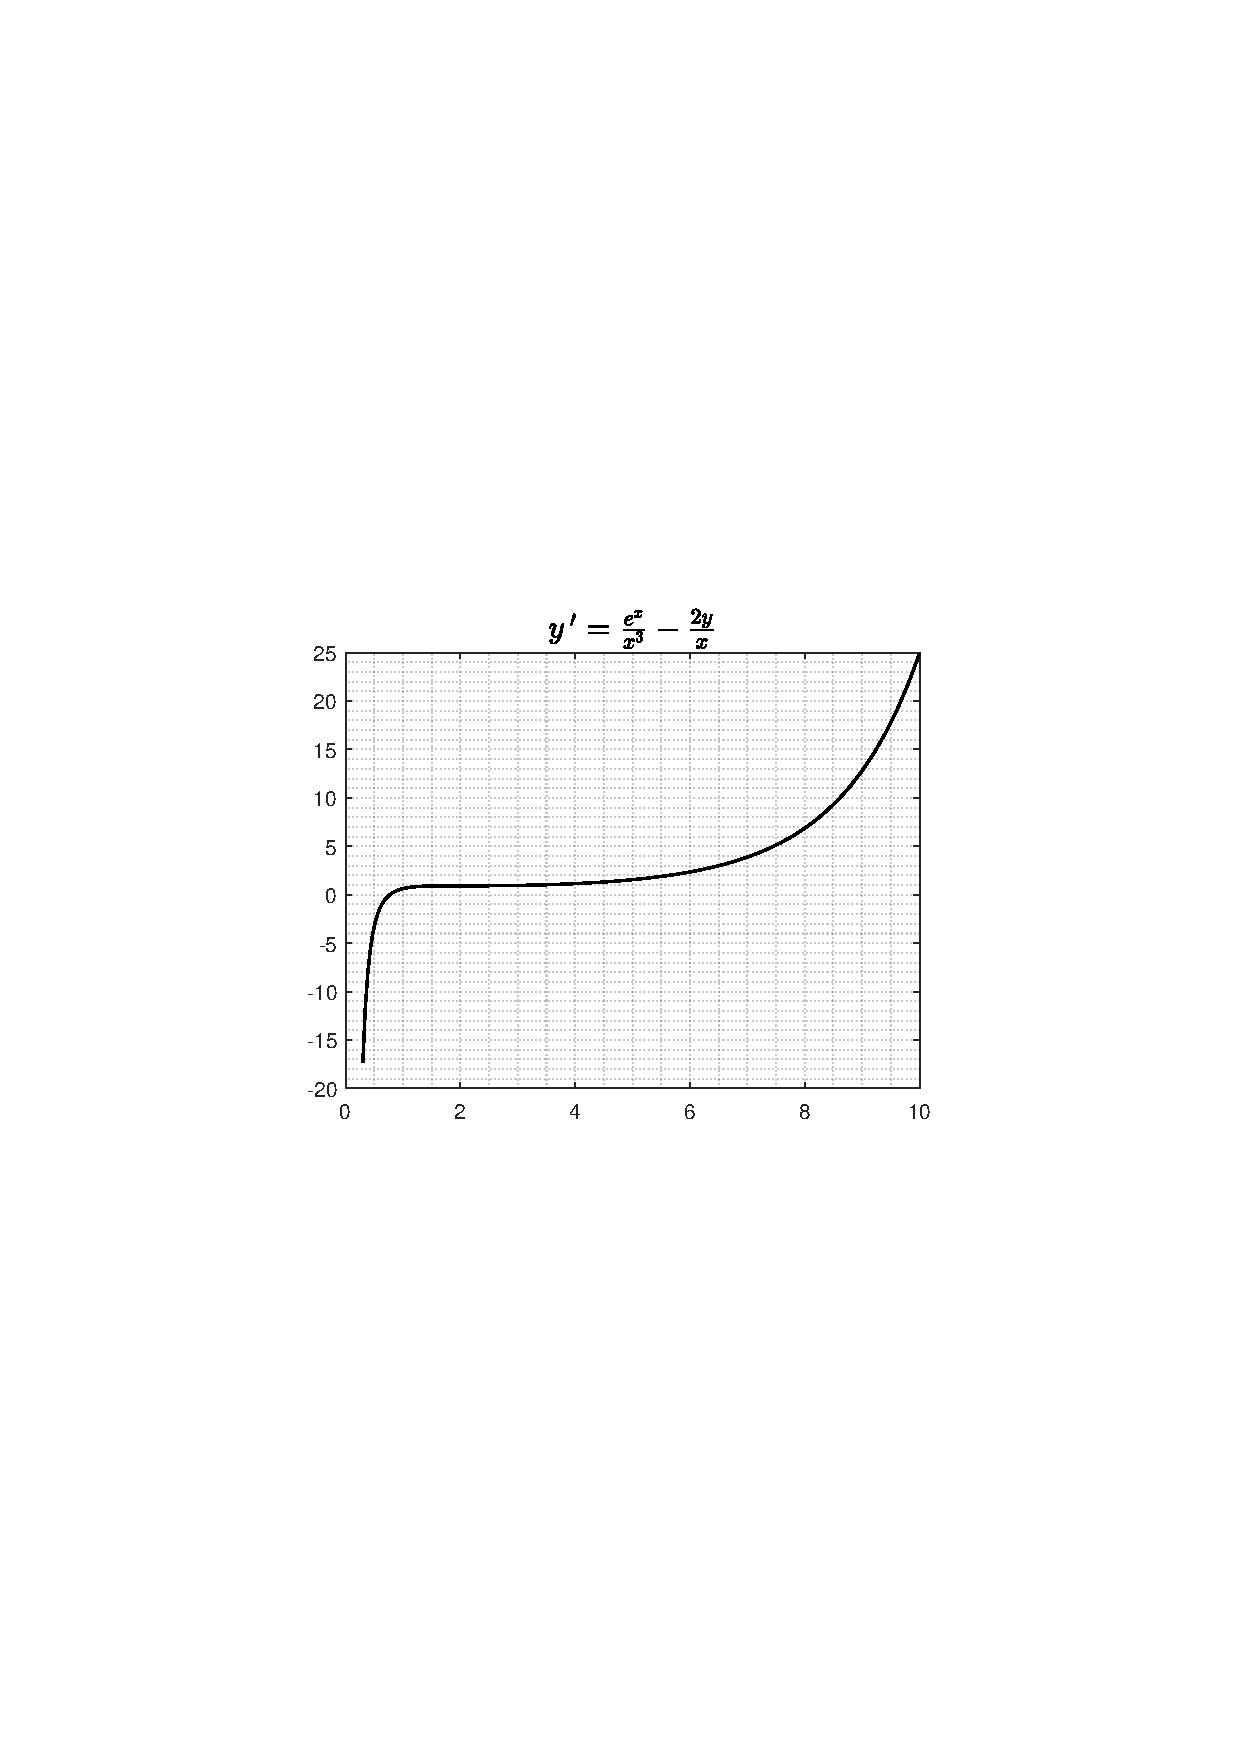
\includegraphics[width=0.6\linewidth]{2013辽宁高考微分方程}
\end{figure}

\item (1) $ y=(a-1)x $. \\
(2) $ f'(x)=a-(x+1)\e^x $,函数$ g(x)=(x+1)\e^x $在
$ (-\infty,-2) $上单调递减,在$ (-2,+\infty) $上单调递增,
当$ x>-1 $时,$ g(x)>0 $,所以$ g(x)=a>0 $只有唯一解,
$ f(x) $存在唯一的极值点。\\
(3) $ a(x-1)-x\e^x\leq b $,令$ h(x)=a(x-1)-x\e^x $,
则$ h'(x)=a-(x+1)\e^x $,设$ h'(x_0)=0 $,则
$ a=(x_0+1)\e^{x_0},\ (x_0>-1) $,$ h(x_0)=(x_0^2-1)
\e^{x_0}-x_0\e^{x_0} $,令$ \varphi(x)=(x^2-x-1)
\e^{x} $,则$ \varphi'(x)=(x+2)(x-1)\e^x $,
当$ x=1 $时,$ \varphi(x) $取得极小值$ -\e $\, (这其实是
$ h(x) $的最大值的最小值)。所以,
$ b $的取值范围是$ [-\e,+\infty) $.

\item 
使用数学归纳法,只需证明
\begin{gather*}
    \Big(\dfrac{n+2}{3}\Big)^{n+1}<\Big(\dfrac{n+1}{3}\Big)^{n}
    \cdot (n+1)<(n+1)!<\Big(\dfrac{n+1}{2}\Big)^{n}\cdot (n+1)<\Big(\dfrac{n+2}{2}\Big)^{n+1}
\end{gather*}
等价于证明$ 2<\Big(1+\dfrac{1}{n}\Big)^{n}<3 $,使用二项式定理即可,
参见(\ref{e小于3的证明})式。

\item 
(I)$ f'(\dfrac{5a}{4})=0,\ f(\dfrac{5a}{4})=\ln \dfrac{5a}{4}+1+\dfrac{a}{4}=\dfrac{6}{5},\ a=\dfrac{4}{5} $.\\
(II)利用$ -\dfrac{4x\ln x}{x+5} $在$ x=1 $处的$ (2,1) $阶帕德逼近可得:$ -\dfrac{4x\ln x}{x+5}>-\dfrac{2x(x-1)}{2x+1}\ (0<x<1) $,记$ -\dfrac{2x(x-1)}{2x+1}=a $的两根为$ x_3,x_4 $,那么$ x_{3,4}=\dfrac{1-2\pm \sqrt{a^2-4a+1}}{2},\  |x_2-x_1|>|x_3-x_4|=\sqrt{a^2-4a+1},\ x_1^2+x_2^2>a^2-4a+1+2x_1x_2>a^2-4a+1 $.

\item 
因为$ a>\e $,$ x\ln x $在$ \Big(\dfrac{1}{\e},+\infty\Big) $
上单调递增,所以$ x_0>\e $,$ a=x_0\ln x_0>x_0 $,$ x_0=\dfrac{a}{\ln x_0}
>\dfrac{a}{\ln a} $. 原不等式左半部分得证。\\
当$ x>1 $时,$ \dfrac{x}{\ln x}\geq \e $,$ x\geq \e\ln x $,将
$ x $换成$ x^{1/r}\ (r>1) $,有$ x^{1/r}\geq \e\ln x^{1/r}=\dfrac{\e}{r}\ln x $.
于是$ a=x_0\ln x_0\leq x_0\cdot \dfrac{r}{\e}x_0^{1/r}=\dfrac{r}{\e}
x_0^{(r+1)/r} $,即
\begin{gather*}
    \dfrac{r}{r+1}\Big(\ln\dfrac{\e}{r}+\ln a\Big)\leq \ln x_0
\end{gather*}
如果
\begin{gather}\label{xlnx零点不等式习题}
    \dfrac{\e}{\e+1}\ln a\leq \dfrac{r}{r+1}\Big(\ln\dfrac{\e}{r}+\ln a\Big)
\end{gather}
成立,那么
\begin{gather*}
    x_0=\dfrac{a}{\ln x_0}\leq \dfrac{a}{\dfrac{r}{r+1}\Big(
        \ln\dfrac{\e}{r}+\ln a\Big)} 
    \leq \dfrac{a}{\dfrac{\e}{\e+1}\ln a}
\end{gather*}
即原不等式右半部分得证。把(\ref{xlnx零点不等式习题})式左右两侧看成关于
$ \ln a $的一次函数,那么$ \dfrac{\e}{\e+1}\leq \dfrac{r}{r+1} $,
解得$ r\geq \e $,取$ r=\e $,那么有$ \dfrac{\e}{\e+1}\ln a\leq x_0 $,
当$ a=\e^{\e+1},\ x_0=\e^{\e} $时,等号成立。证毕。

\item 
令$ f(x)=\cos x+\dfrac{4x^2}{\pi^2} $,则
$ f'(x) =-\sin x+\dfrac{8x}{\pi^2} $,
$ f''(x)=-\cos x+\dfrac{8}{\pi^2} $.\\
设$ f''(x_2)=0 $,因为$ \dfrac{8}{\pi^2}>\dfrac{8}{10}>\dfrac{\sqrt{2}}{2} $,
所以$ x_2=\arccos\dfrac{8}{\pi^2}<\arccos\dfrac{\sqrt{2}}{2}=\dfrac{\pi}{4} $,
(借助软件可算出$ x_2=0.625672\cdots $),$ f'(x) $在$ (0,x_2) $上单调递减,
在$ \Big(x_2,\dfrac{\pi}{2}\Big) $上单调递增,$ f'(0)=0 $,
$ f'\Big(\dfrac{\pi}{4}\Big)
=\dfrac{\sqrt{2}(2\sqrt{2}-\pi)}{2\pi}<0 $,$ f'\Big(\dfrac{\pi}{2}\Big)
=-1+\dfrac{4}{\pi}>0 $.所以,$ f'(x) $在$ \big(0,\dfrac{\pi}{2}\big) $
上有且仅有一个零点,设为$ x_1 $,显然有$ x_1\in\Big(\dfrac{\pi}{4},
\dfrac{\pi}{2}\Big) $(借助软件可算出$ x_1=1.098824\cdots $).
又有$ f(x) $在$ (0,x_1) $上单调递减,在
$ \Big(x_1,\dfrac{\pi}{2}\Big) $上单调递增,$ x_1 $是$ f(x) $
的极小值点。因为$ f(0)=1,\ f(1)=1 $,所以$ f(x)<1 $
在$ \Big(0,\dfrac{\pi}{2}\Big) $上恒成立。证毕。

\item 
(1) $ \dfrac{\partial z}{\partial x}=\dfrac{2x}{x^2+y^2},\ 
\dfrac{\partial z}{\partial y}=\dfrac{2y}{x^2+y^2} $. \quad
(2) $ \dfrac{\partial z}{\partial x}=\dfrac{x}{\sqrt{x^2+y^2}},\ 
\dfrac{\partial z}{\partial y}=\dfrac{y}{\sqrt{x^2+y^2}} $. \\
(3) $ \dfrac{\partial z}{\partial x}=4x^3+6y^3,\ 
\dfrac{\partial z}{\partial x}=18xy^2-5y^4 $. \\
(4) $ \dfrac{\partial z}{\partial x}=\e^x[\sin(x+y^2)+\cos(x+y^2)],\ 
\dfrac{\partial z}{\partial y}=2ye^x \cos(x+y^2) $. 

\item (1) $ \dfrac{\partial u}{\partial x} =
\dfrac{-x^2+y^2}{(x^2+y^2)^2}=\dfrac{\partial v}{\partial y} $,
$ \dfrac{\partial v}{\partial x} =\dfrac{2xy}{(x^2+y^2)^2}=
-\dfrac{\partial u}{\partial y} $. \\
(2) $ \dfrac{\partial u}{\partial x} =\e^x \cos y=
\dfrac{\partial v}{\partial y} $,
$ \dfrac{\partial v}{\partial x} =\e^x \sin y=
-\dfrac{\partial u}{\partial y} $. \\
(3) $ \dfrac{\partial u}{\partial x} =\cos x\cosh y=
\dfrac{\partial v}{\partial y} $,
$ \dfrac{\partial v}{\partial x} = -\sin x\sinh y=
-\dfrac{\partial u}{\partial y} $. 

\item 略

\end{enumerate}
%$ \displaystyle\int_0^1x^xdx=\sum_{k=1}^{\infty}\dfrac{(-1)^{n+1}}{n^n},\
%\int_0^1\dfrac{1}{x^x}dx = \sum_{k=1}^{\infty}\dfrac{1}{n^n} $.
\myfootnote{\CopyrightStatementChap}
% {\footnotesize (可在以下空白区域自行增补知识点。)}  
\cleardoublepage

%~\newpage
%~\newpage

%------------------------------------------

